\documentclass[10pt]{article}
\usepackage[margin=0.65in]{geometry}
\usepackage[T1]{fontenc}
\usepackage{lmodern}
\usepackage{graphicx}
\usepackage{pdfpages}
\usepackage[hidelinks]{hyperref}
\setlength{\parindent}{0pt}
\setlength{\parskip}{5pt}
\title{NeuraEdge Universal: Deep Debug Plots and Waveforms}
\author{Generated from CIFAR-10, XSim, compiler, and Vivado artifacts}
\date{\today}
\begin{document}
\maketitle
\tableofcontents
\clearpage
\section{Evidence rule}
Every page names its source artifact. CIFAR-10 plots use all 10,000 official test samples. Waveforms are generated by Vivado 2026.1 XSim from repository testbenches. Timing and power pages are included only when the corresponding routed report exists. A Vivado estimate is not relabeled as a physical board measurement.
\clearpage
\section{Native Vivado PYNQ block design}
This page is exported directly from the validated system.bd block design by Vivado 2026.1. It is not a redrawn or inferred schematic.
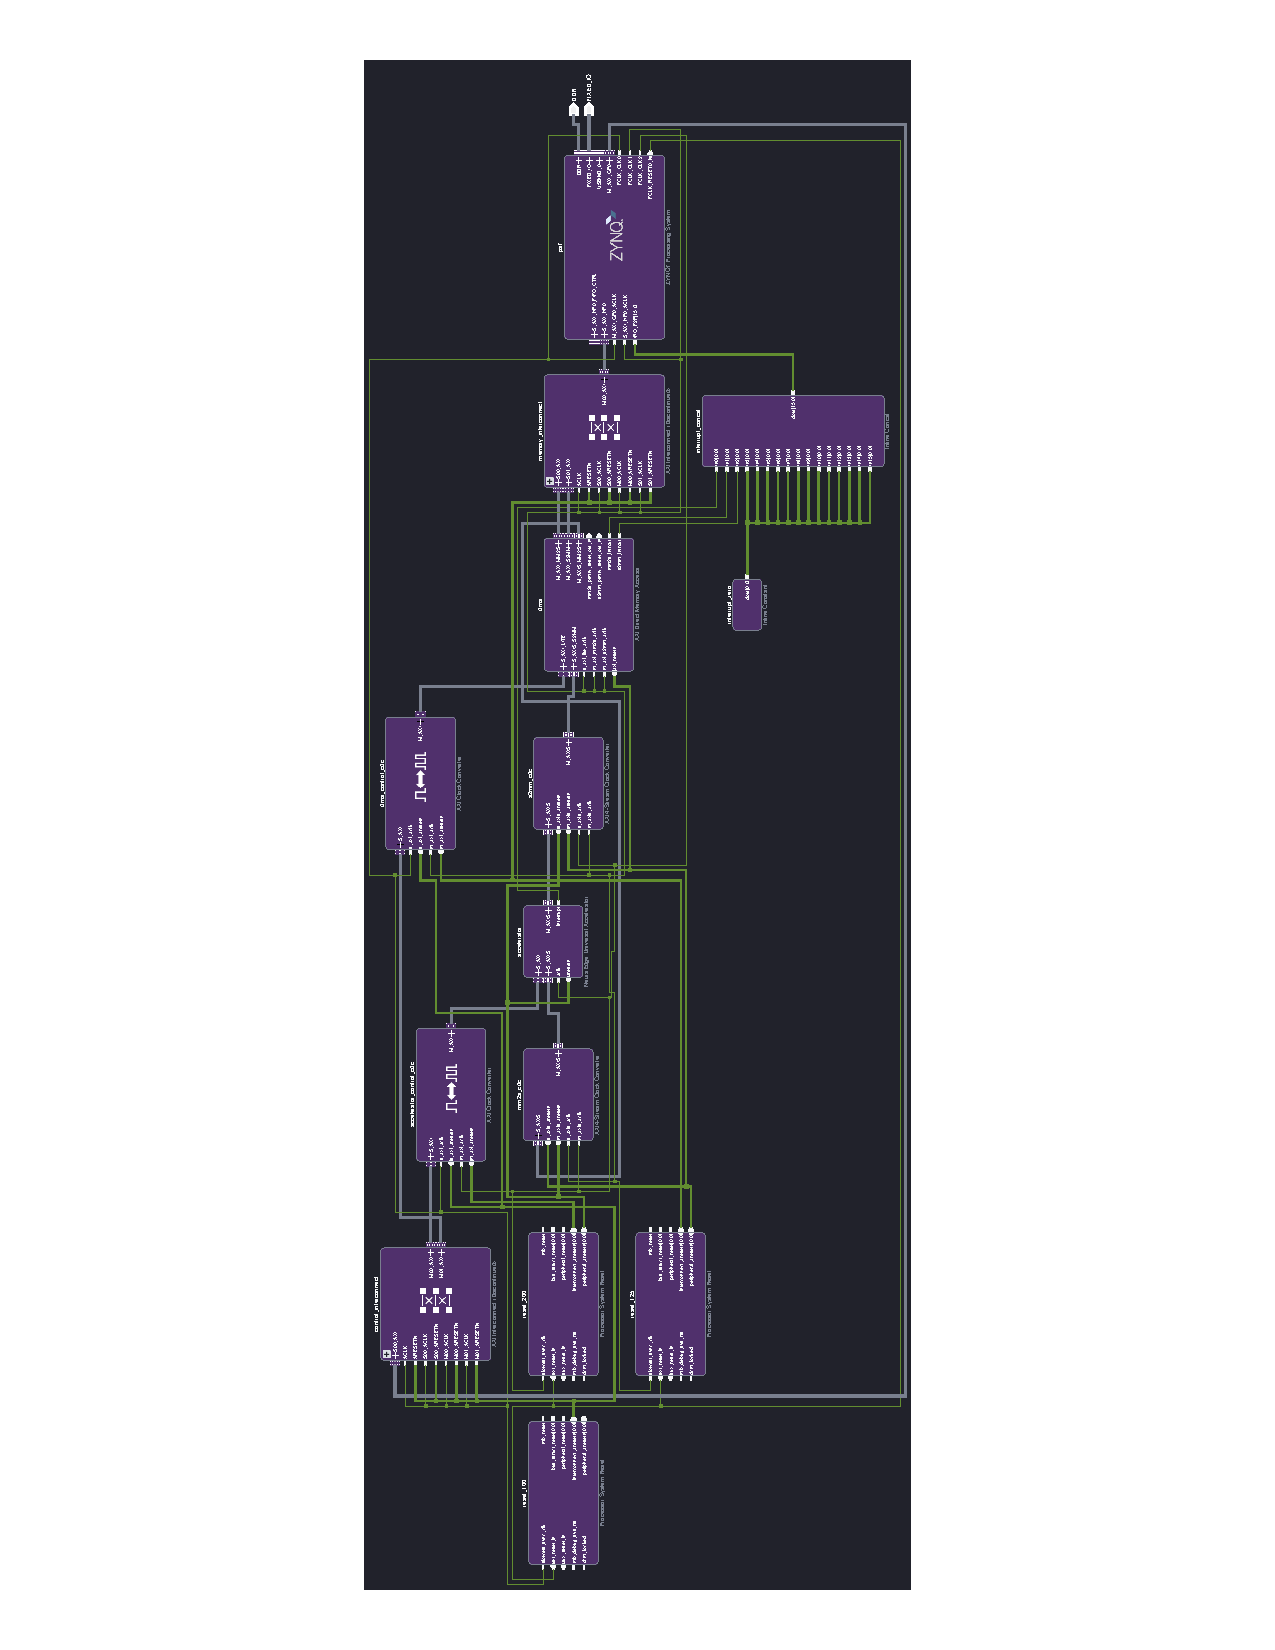
\includepdf[pages=-,fitpaper=true,angle=90,pagecommand={}]{pynq-block-design.pdf}
\clearpage
\section{Measured evidence summary}
\begin{sloppypar}\small\textbf{Evidence:} evaluation JSON,\allowbreak{} execution manifest,\allowbreak{} parameter manifest\end{sloppypar}
\begin{center}
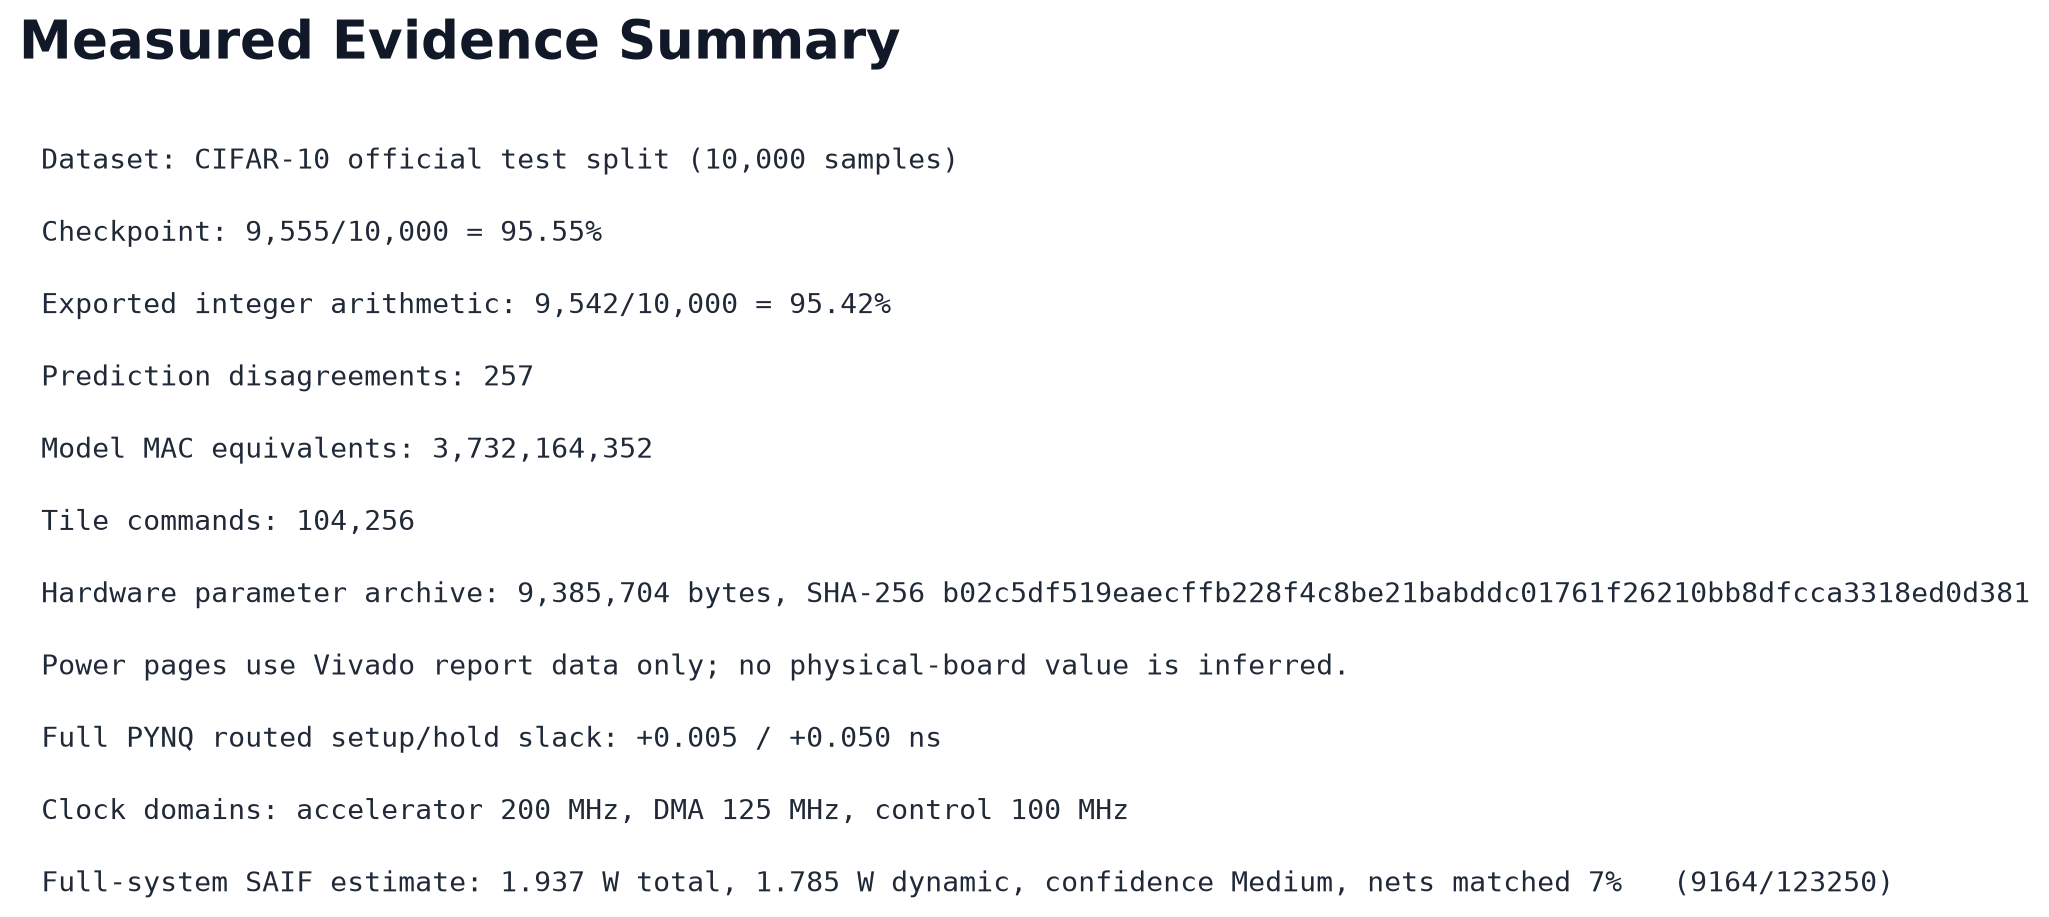
\includegraphics[width=0.98\textwidth,height=0.78\textheight,keepaspectratio]{plots/01_evidence_summary.png}
\end{center}
\clearpage
\section{Complete exported-graph trace validation}
\begin{sloppypar}\small\textbf{Evidence:} C:\textbackslash{}\allowbreak{}Users\textbackslash{}\allowbreak{}Ross\textbackslash{}\allowbreak{}Downloads\textbackslash{}\allowbreak{}neuraedge--main\textbackslash{}\allowbreak{}neuraedge--main\textbackslash{}\allowbreak{}neuraedge\_\allowbreak{}universal\textbackslash{}\allowbreak{}outputs\textbackslash{}\allowbreak{}regression\textbackslash{}\allowbreak{}real\_\allowbreak{}full\_\allowbreak{}graph\_\allowbreak{}forward\_\allowbreak{}validation.json\end{sloppypar}
\begin{center}
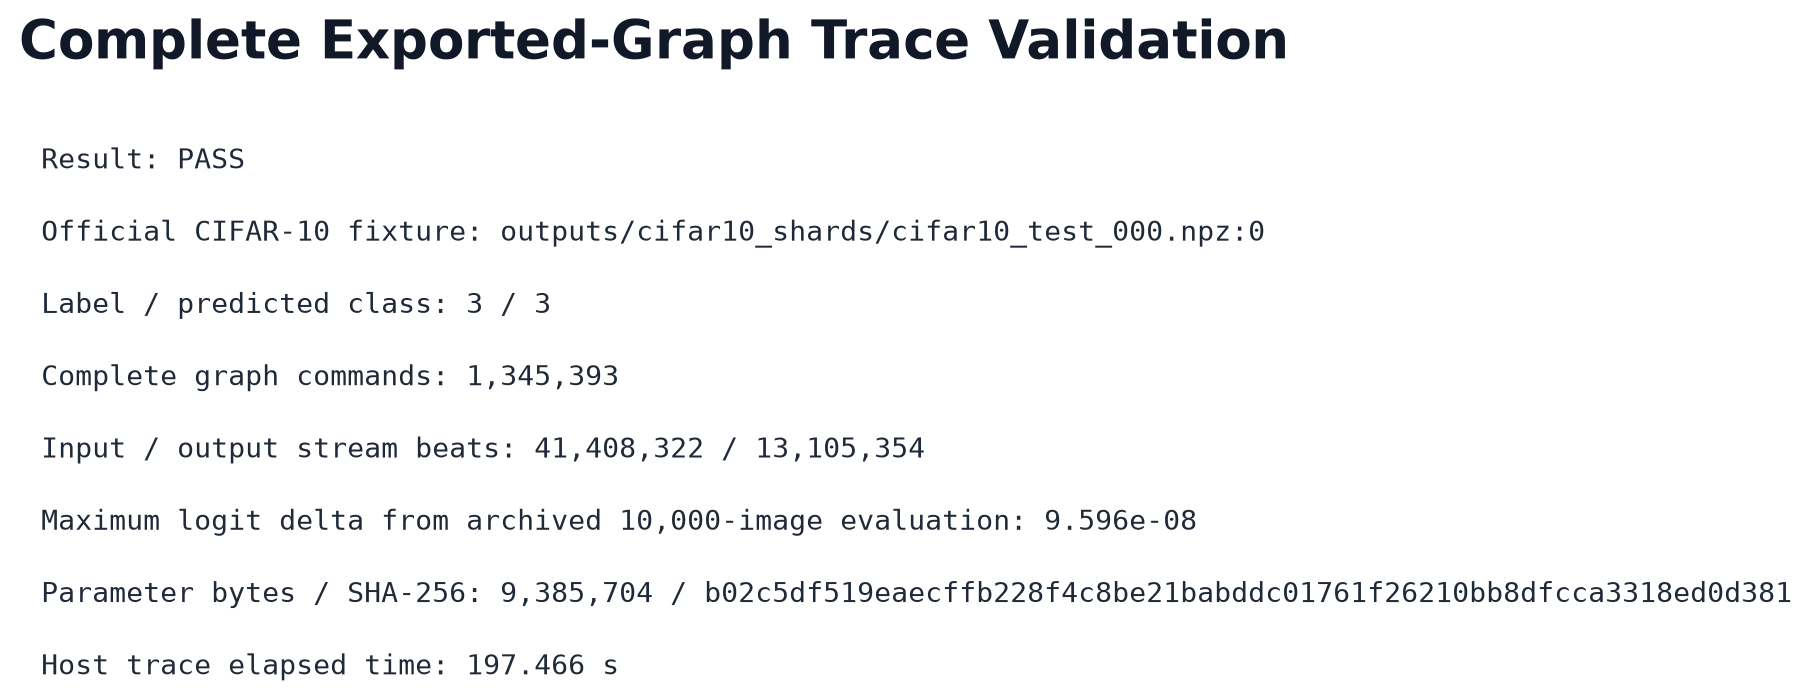
\includegraphics[width=0.98\textwidth,height=0.78\textheight,keepaspectratio]{plots/02_full_graph_validation.png}
\end{center}
\clearpage
\section{Final PYNQ artifact integrity}
\begin{sloppypar}\small\textbf{Evidence:} C:\textbackslash{}\allowbreak{}Users\textbackslash{}\allowbreak{}Ross\textbackslash{}\allowbreak{}Downloads\textbackslash{}\allowbreak{}neuraedge--main\textbackslash{}\allowbreak{}neuraedge--main\textbackslash{}\allowbreak{}neuraedge\_\allowbreak{}universal\textbackslash{}\allowbreak{}outputs\textbackslash{}\allowbreak{}pynq\_\allowbreak{}full\end{sloppypar}
\begin{center}
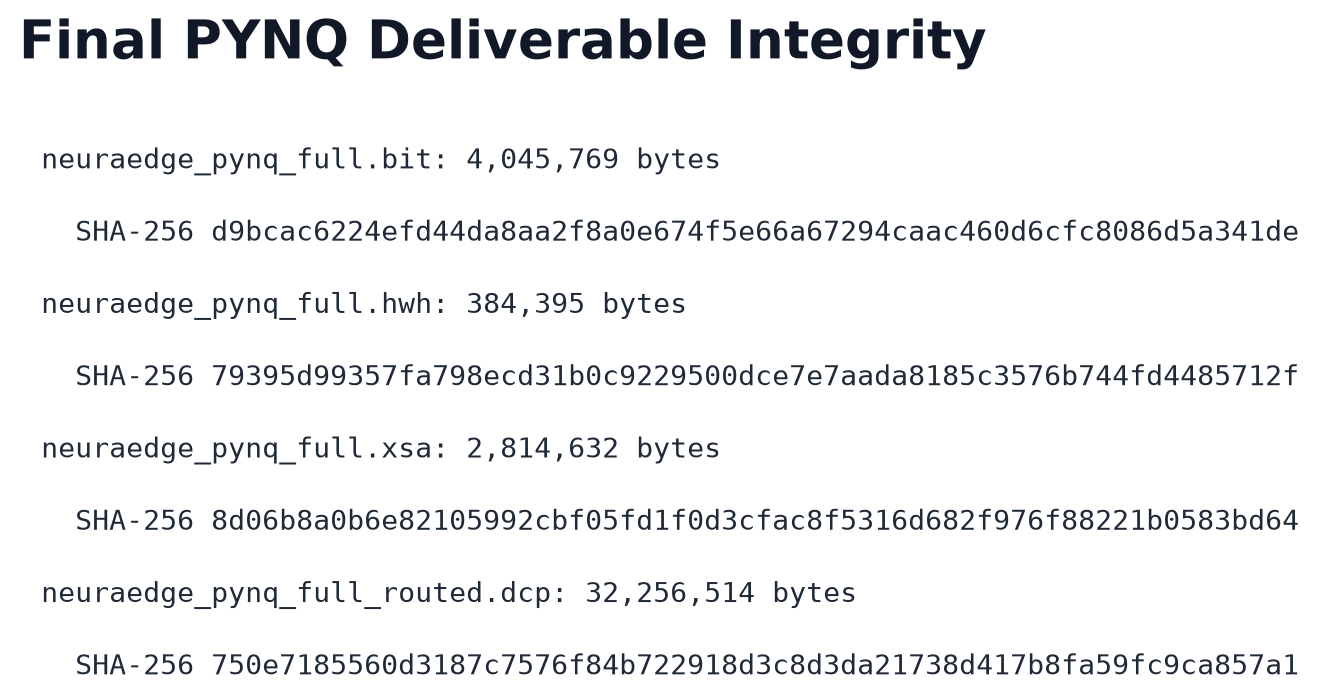
\includegraphics[width=0.98\textwidth,height=0.78\textheight,keepaspectratio]{plots/03_artifact_integrity.png}
\end{center}
\clearpage
\section{Checkpoint confusion matrix: 10,000 images}
\begin{sloppypar}\small\textbf{Evidence:} full CIFAR-10 prediction NPZ/\allowbreak{}JSON\end{sloppypar}
\begin{center}
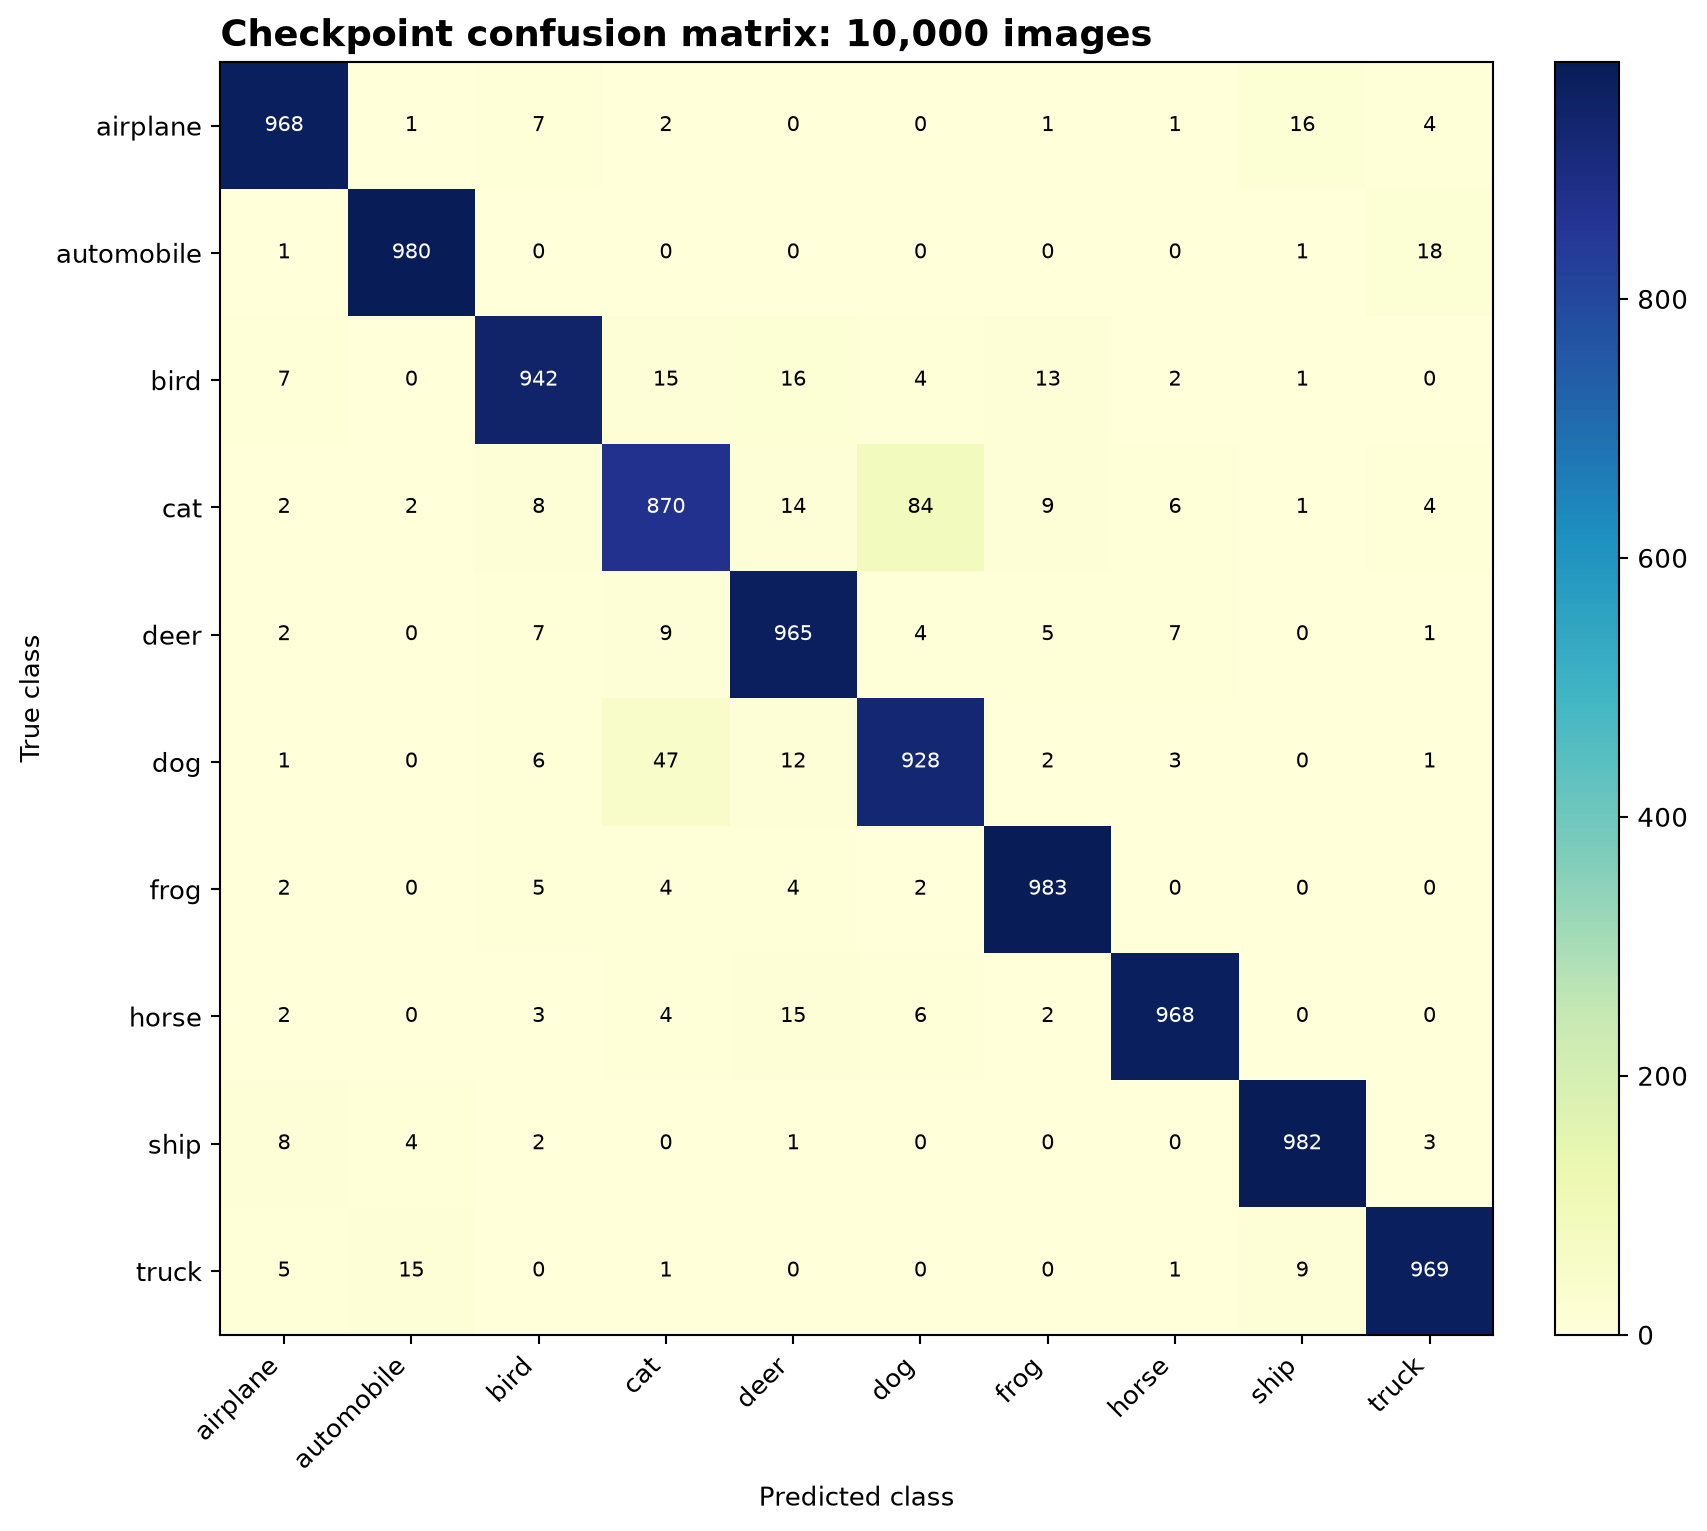
\includegraphics[width=0.98\textwidth,height=0.78\textheight,keepaspectratio]{plots/04_float_confusion.png}
\end{center}
\clearpage
\section{Exported integer confusion matrix: 10,000 images}
\begin{sloppypar}\small\textbf{Evidence:} full CIFAR-10 prediction NPZ/\allowbreak{}JSON\end{sloppypar}
\begin{center}
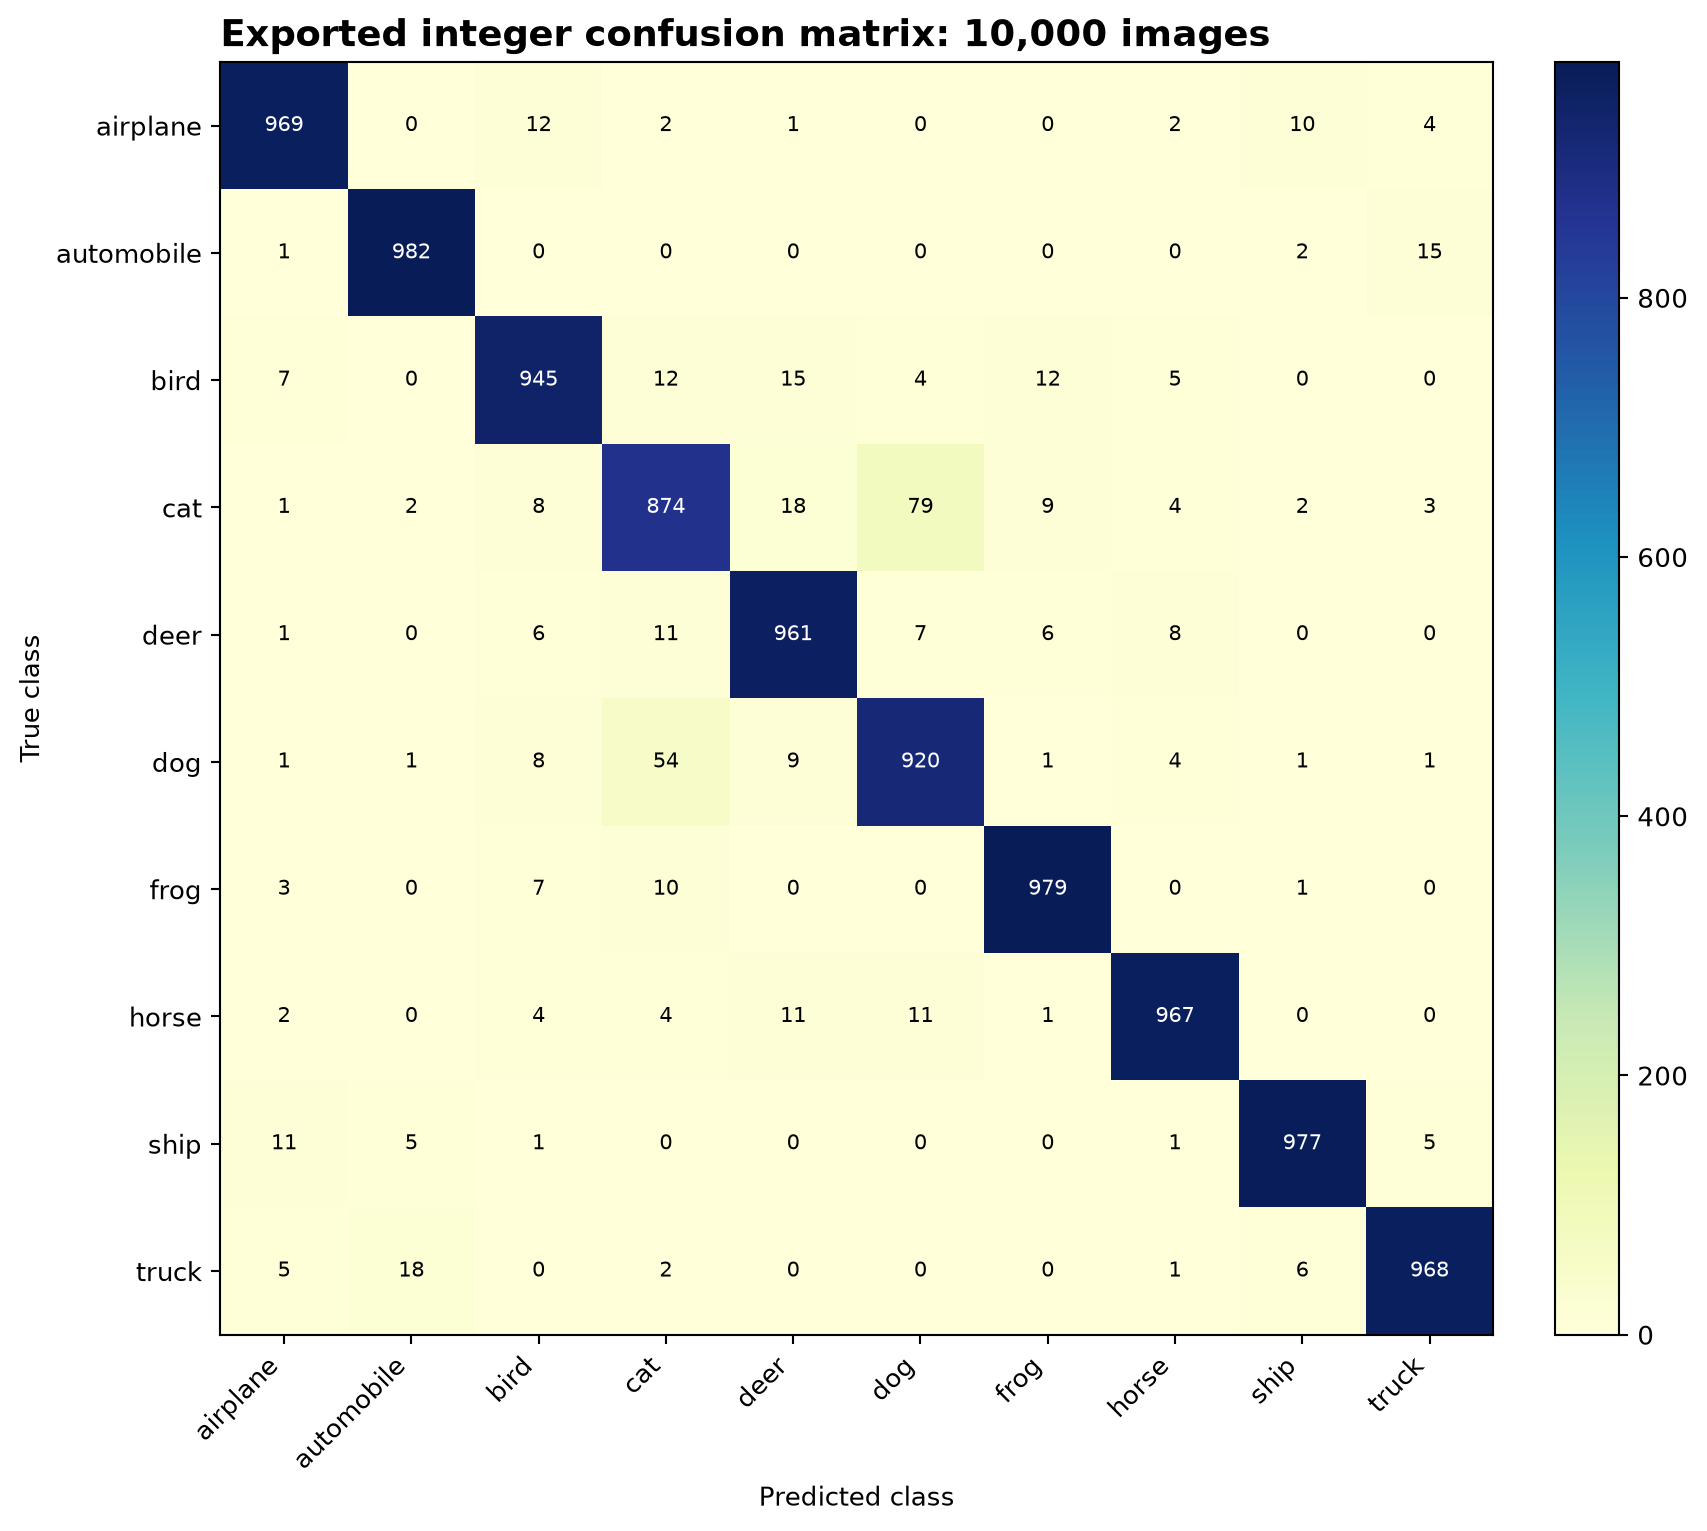
\includegraphics[width=0.98\textwidth,height=0.78\textheight,keepaspectratio]{plots/05_quant_confusion.png}
\end{center}
\clearpage
\section{Integer minus checkpoint confusion counts}
\begin{sloppypar}\small\textbf{Evidence:} full CIFAR-10 prediction NPZ/\allowbreak{}JSON\end{sloppypar}
\begin{center}
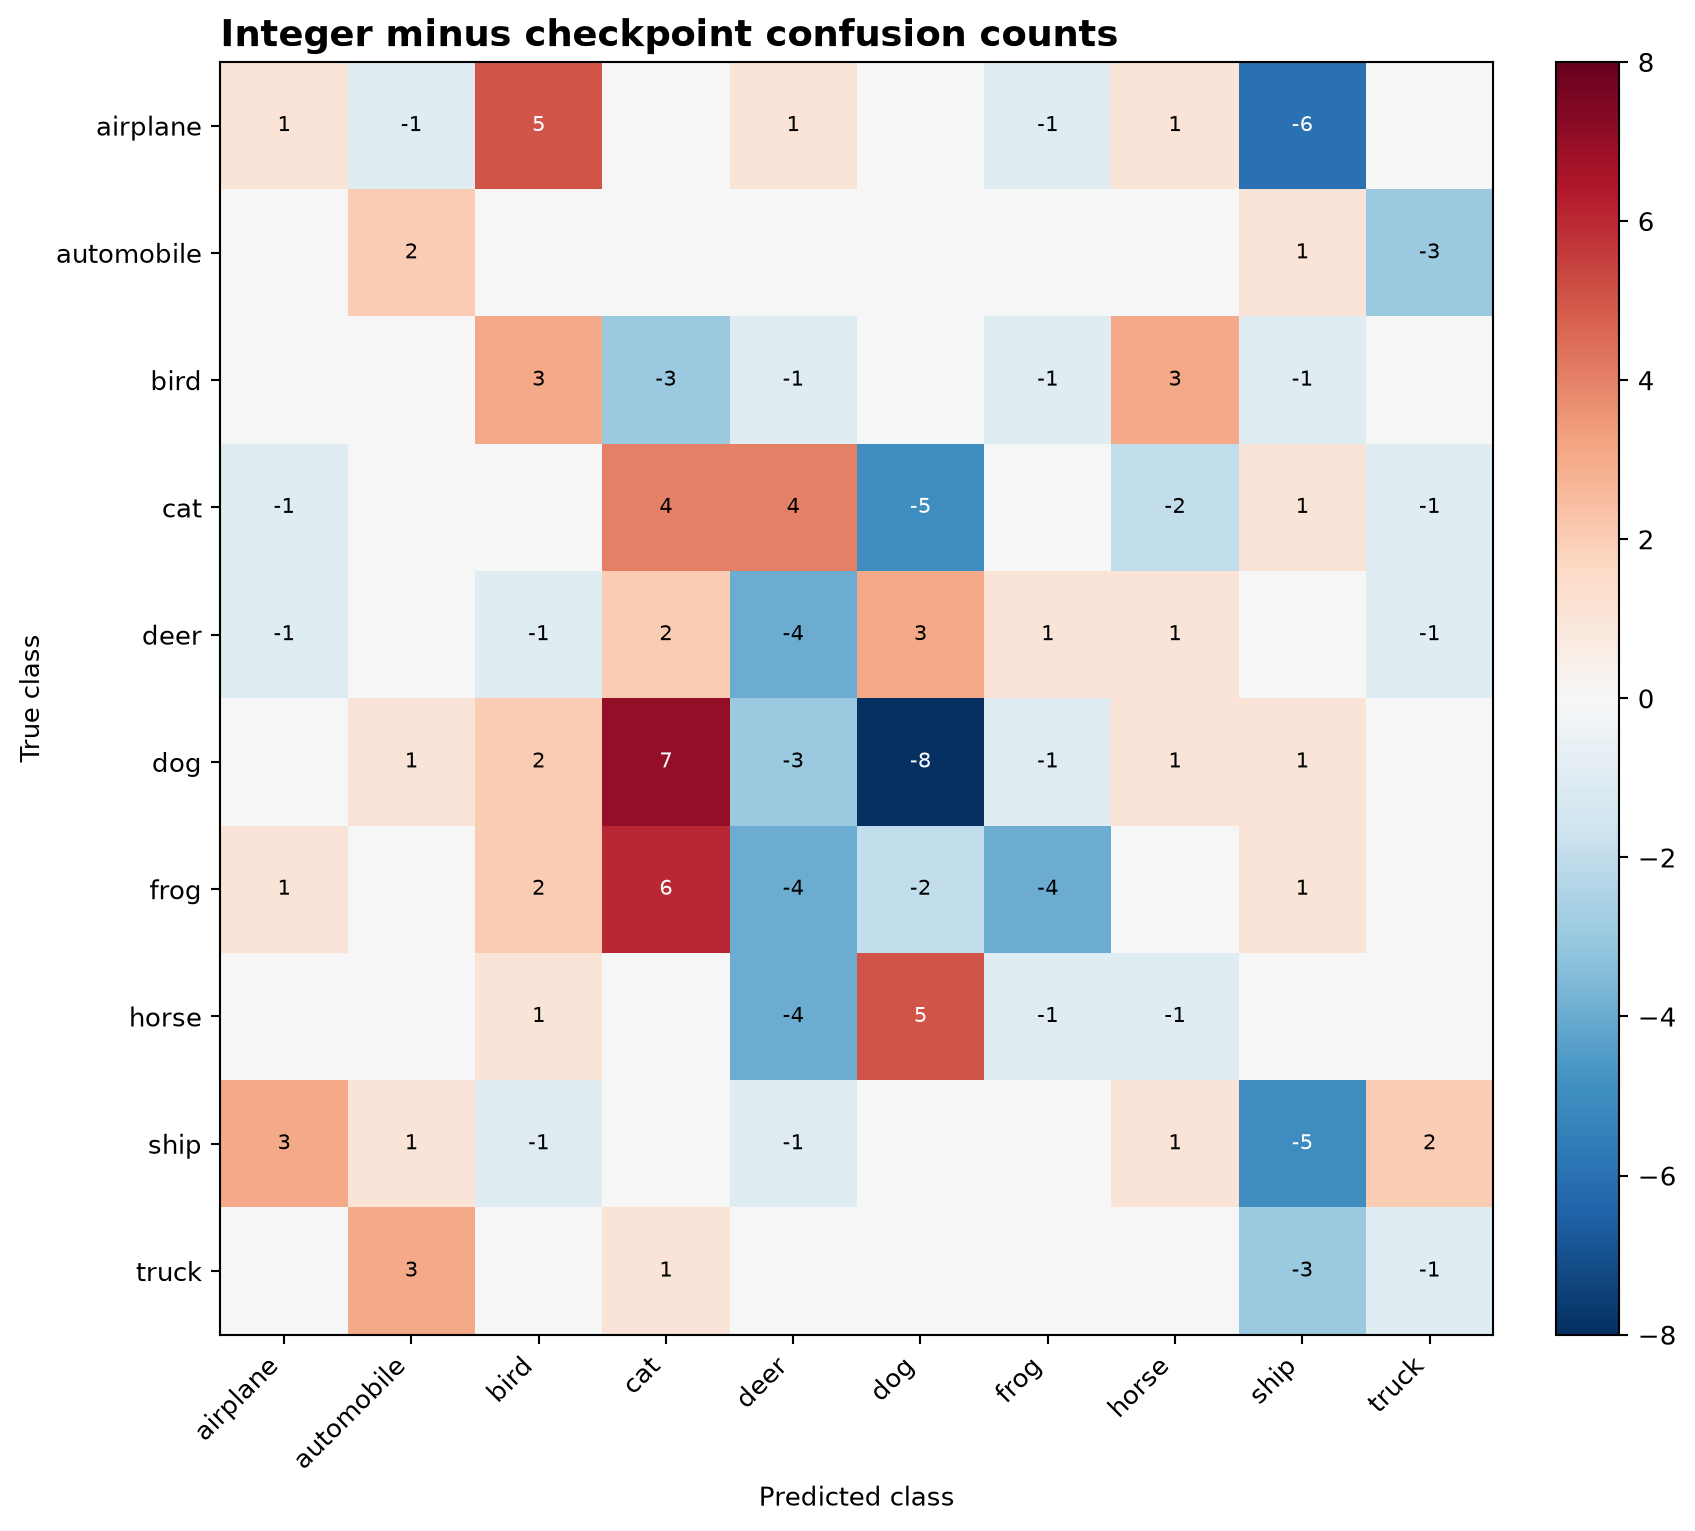
\includegraphics[width=0.98\textwidth,height=0.78\textheight,keepaspectratio]{plots/06_confusion_delta.png}
\end{center}
\clearpage
\section{Per-class top-1 accuracy}
\begin{sloppypar}\small\textbf{Evidence:} full CIFAR-10 confusion matrices\end{sloppypar}
\begin{center}
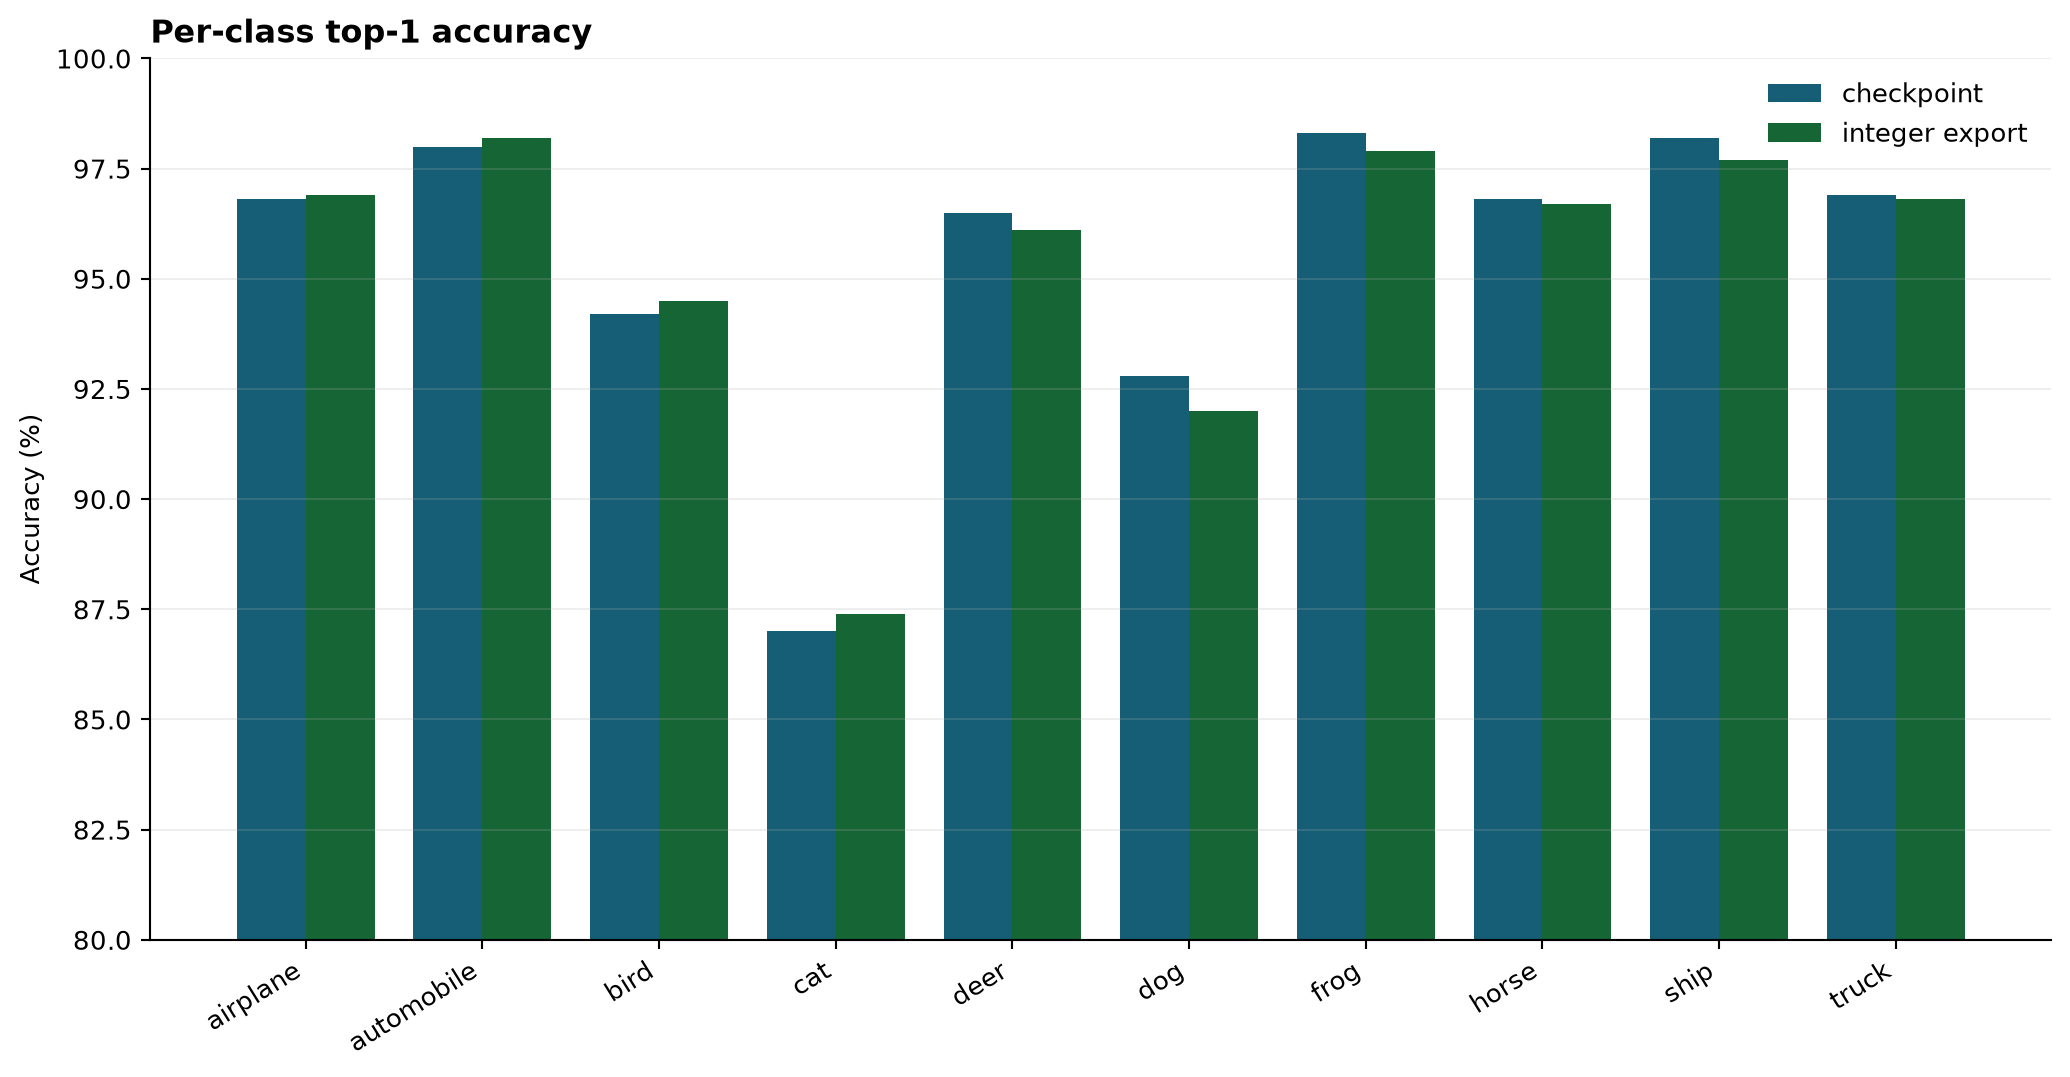
\includegraphics[width=0.98\textwidth,height=0.78\textheight,keepaspectratio]{plots/07_class_accuracy.png}
\end{center}
\clearpage
\section{Classifier margin distribution}
\begin{sloppypar}\small\textbf{Evidence:} all 10,000 checkpoint and integer logits\end{sloppypar}
\begin{center}
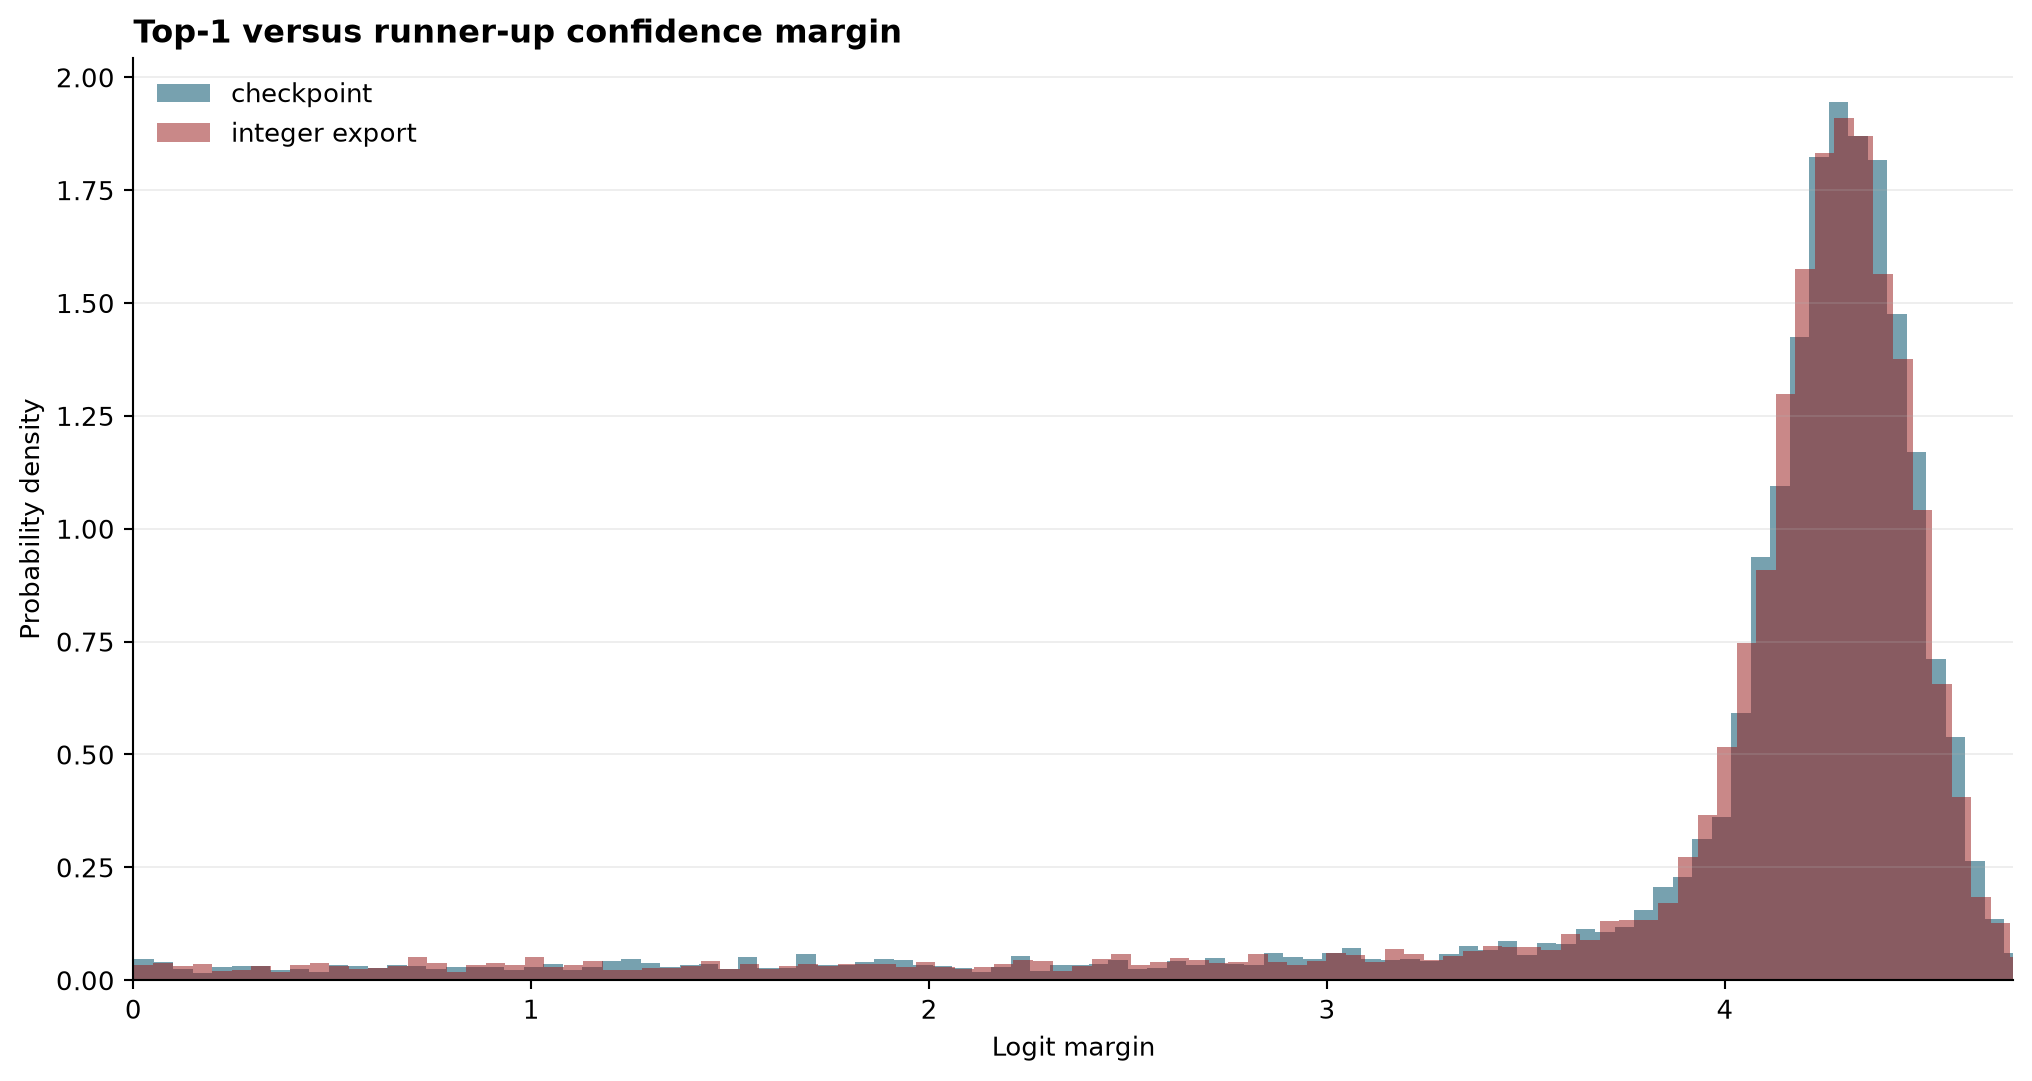
\includegraphics[width=0.98\textwidth,height=0.78\textheight,keepaspectratio]{plots/08_margin_distribution.png}
\end{center}
\clearpage
\section{Integer-export logit error}
\begin{sloppypar}\small\textbf{Evidence:} paired 10,000 x 10 logit arrays\end{sloppypar}
\begin{center}
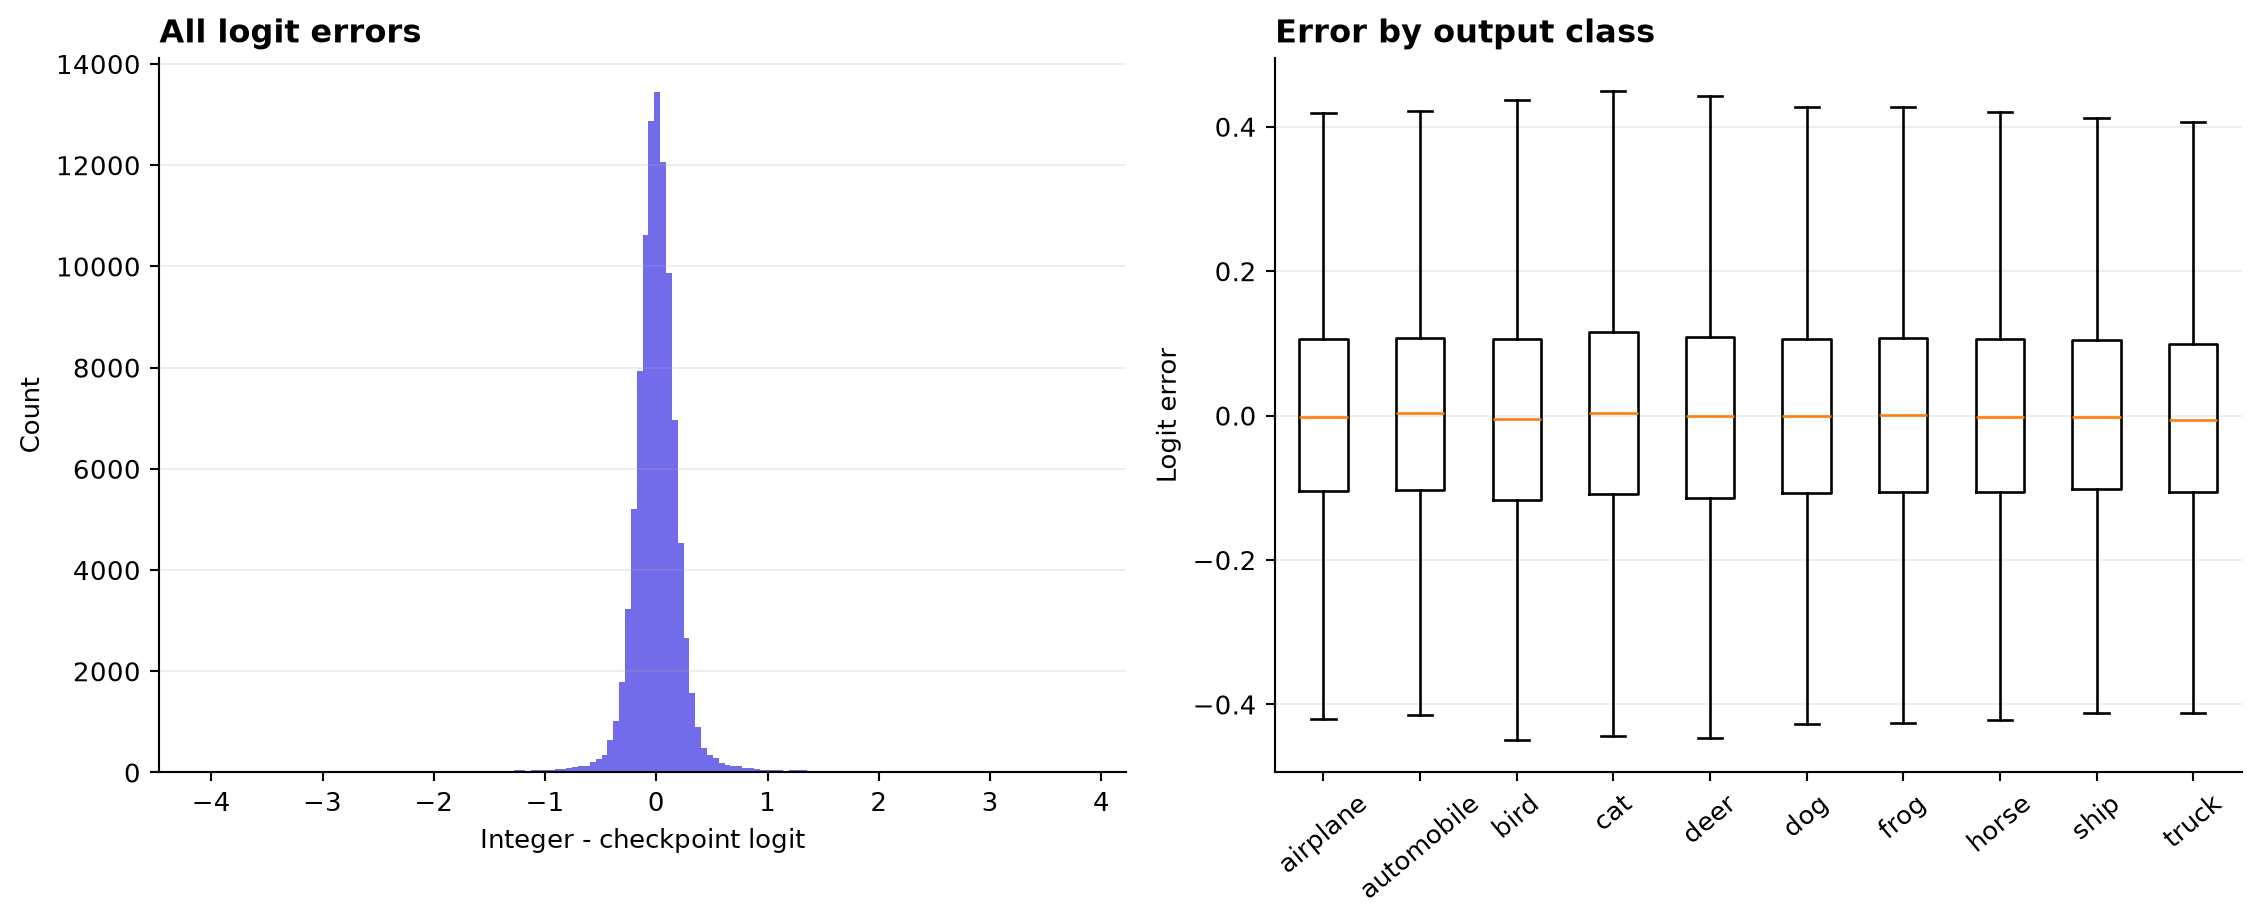
\includegraphics[width=0.98\textwidth,height=0.78\textheight,keepaspectratio]{plots/09_logit_error.png}
\end{center}
\clearpage
\section{Prediction disagreement transitions}
\begin{sloppypar}\small\textbf{Evidence:} 257 changed predictions from paired NPZ files\end{sloppypar}
\begin{center}
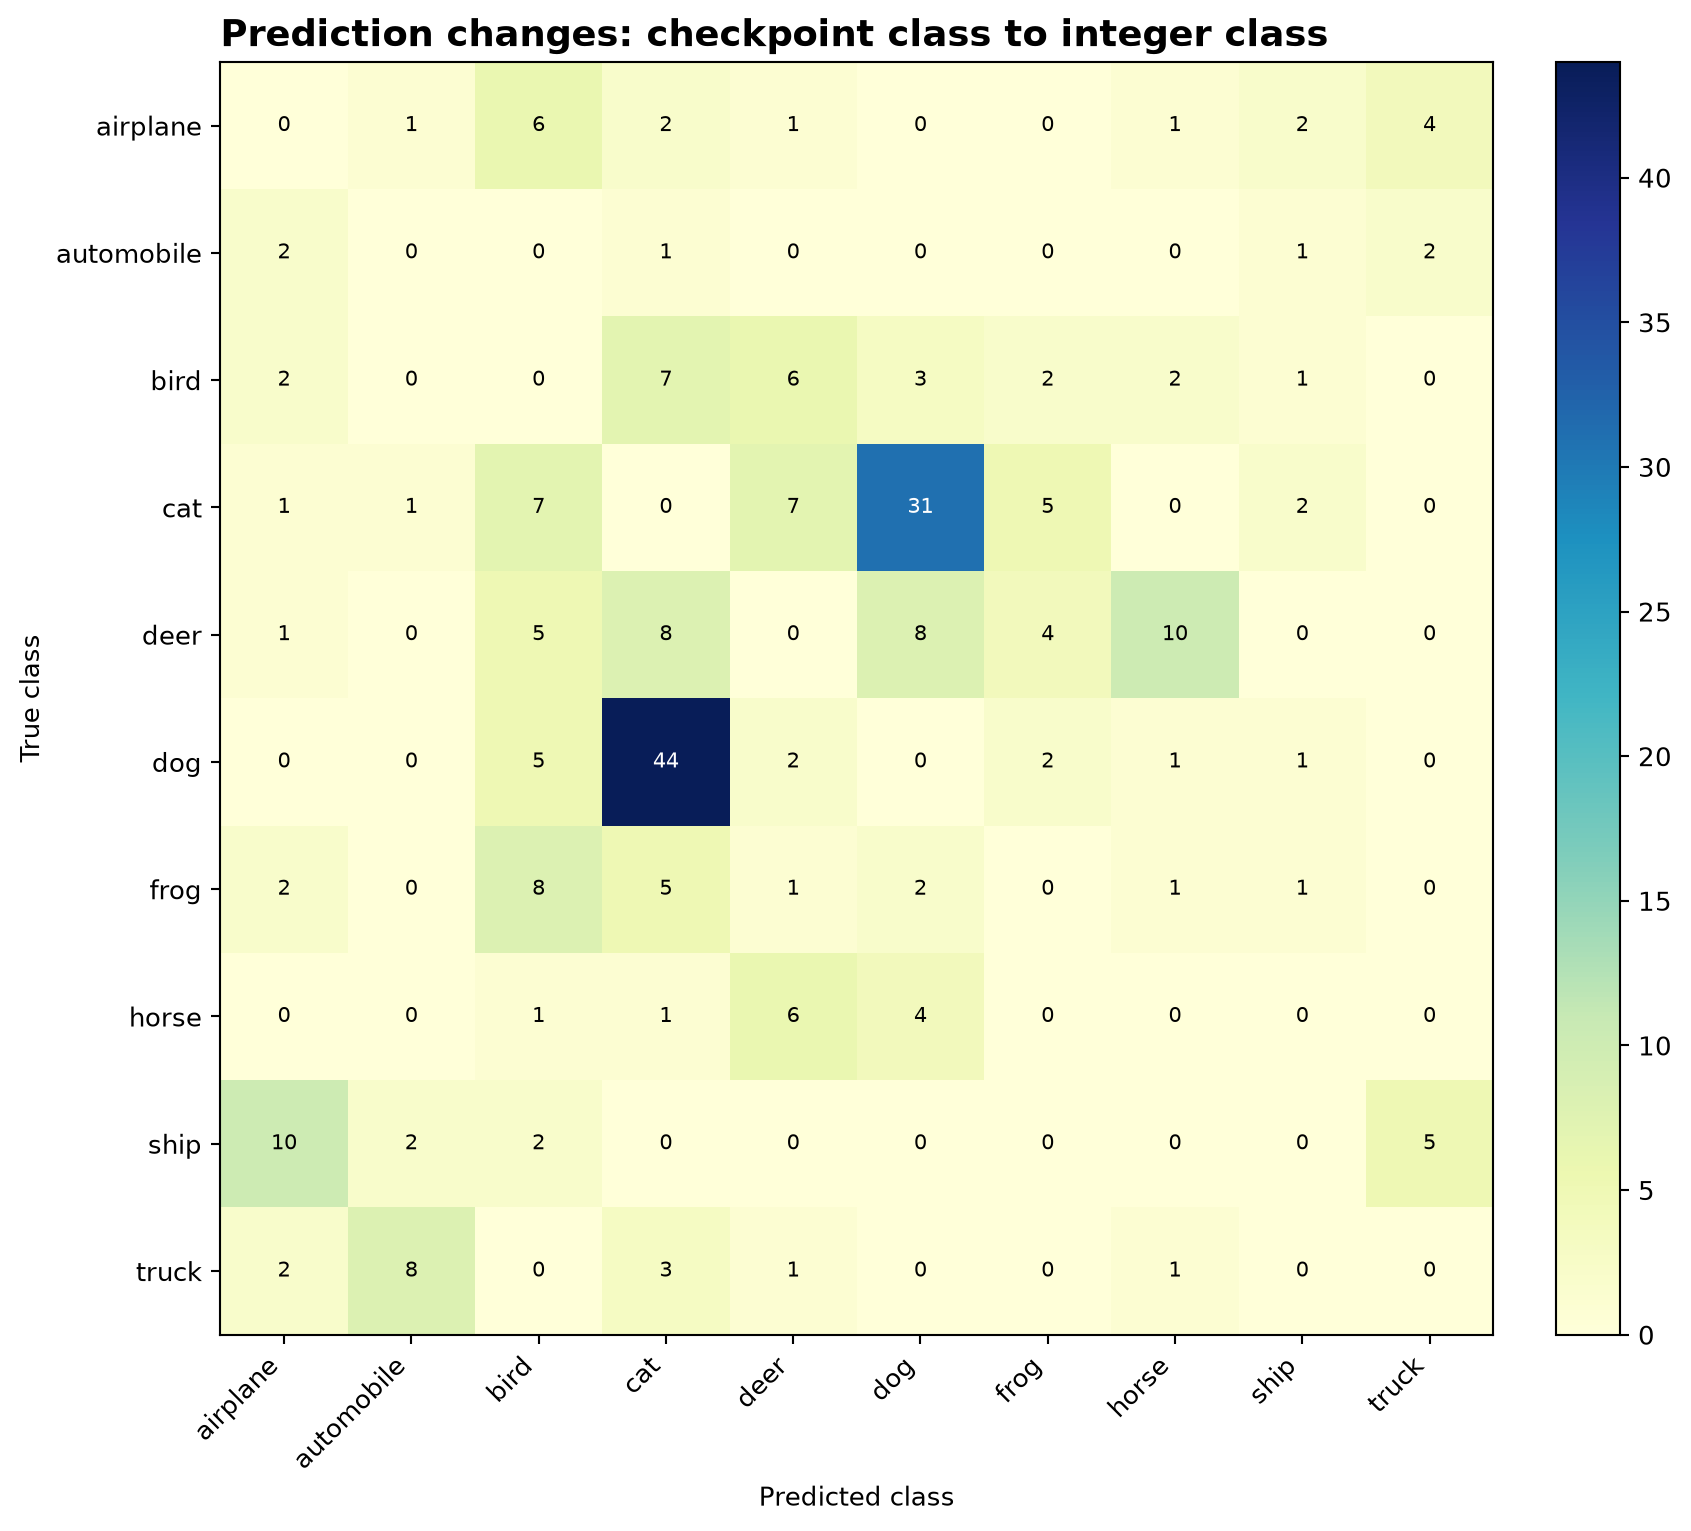
\includegraphics[width=0.98\textwidth,height=0.78\textheight,keepaspectratio]{plots/10_prediction_changes.png}
\end{center}
\clearpage
\section{Measured spike density}
\begin{sloppypar}\small\textbf{Evidence:} streaming activation statistics over all CIFAR-10 test images\end{sloppypar}
\begin{center}
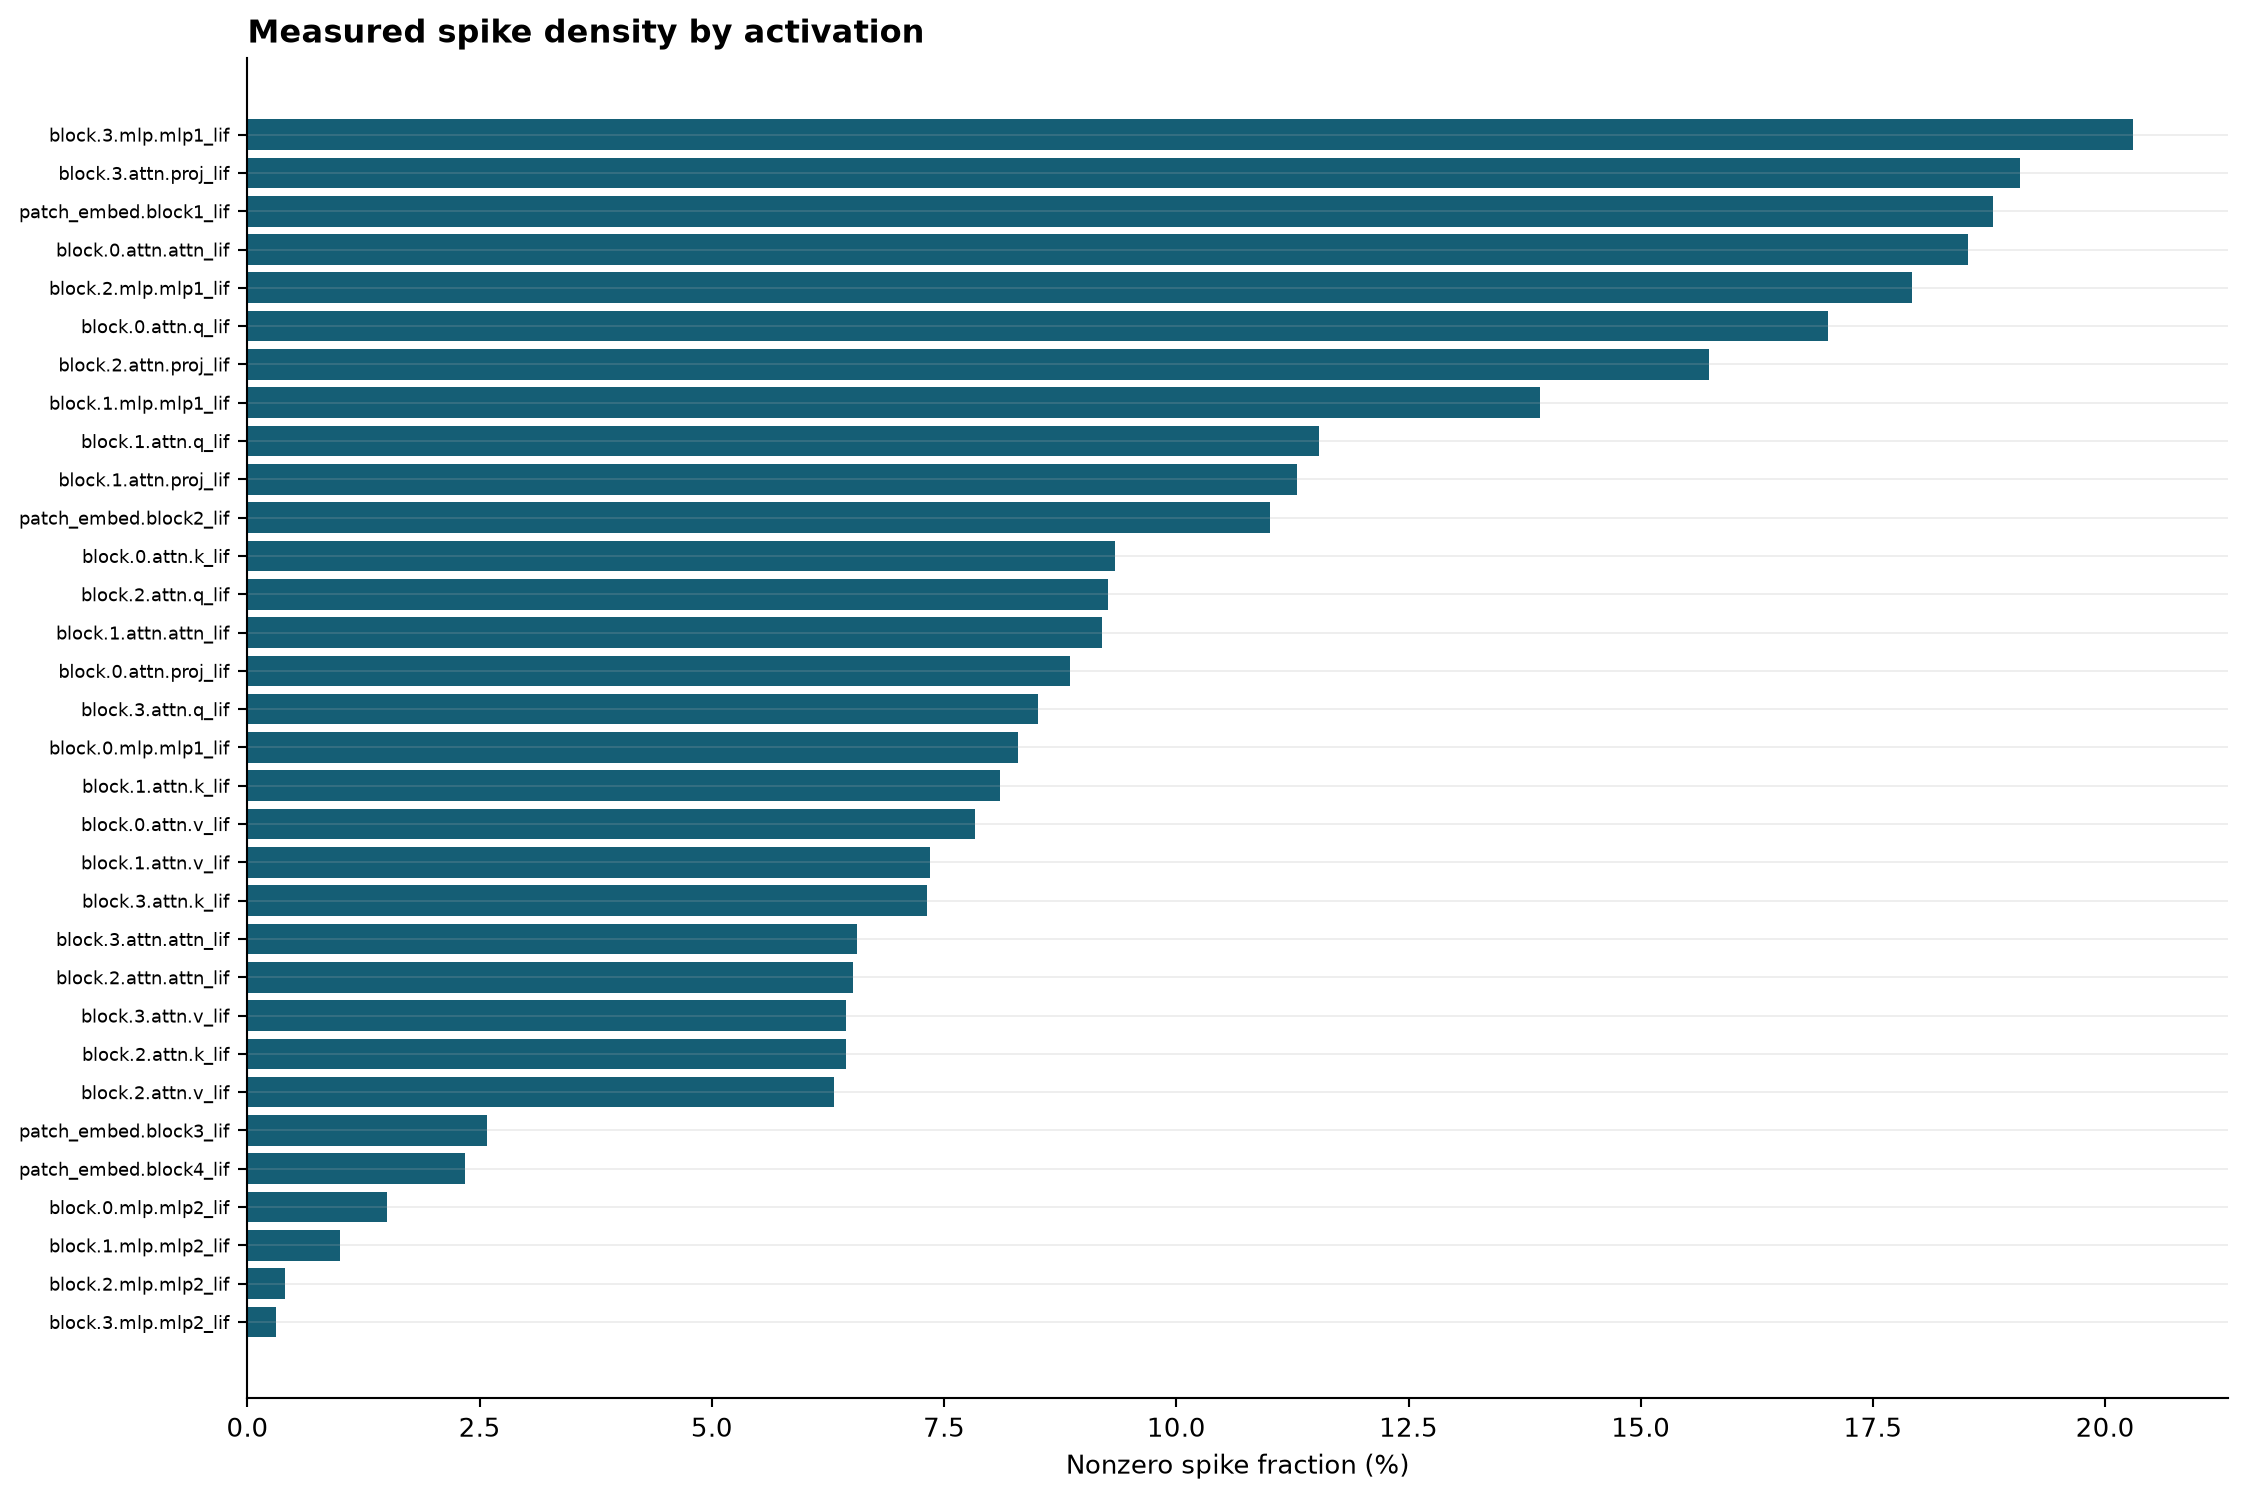
\includegraphics[width=0.98\textwidth,height=0.78\textheight,keepaspectratio]{plots/11_spike_density.png}
\end{center}
\clearpage
\section{Q/K/V spike density}
\begin{sloppypar}\small\textbf{Evidence:} full-test streaming activation statistics\end{sloppypar}
\begin{center}
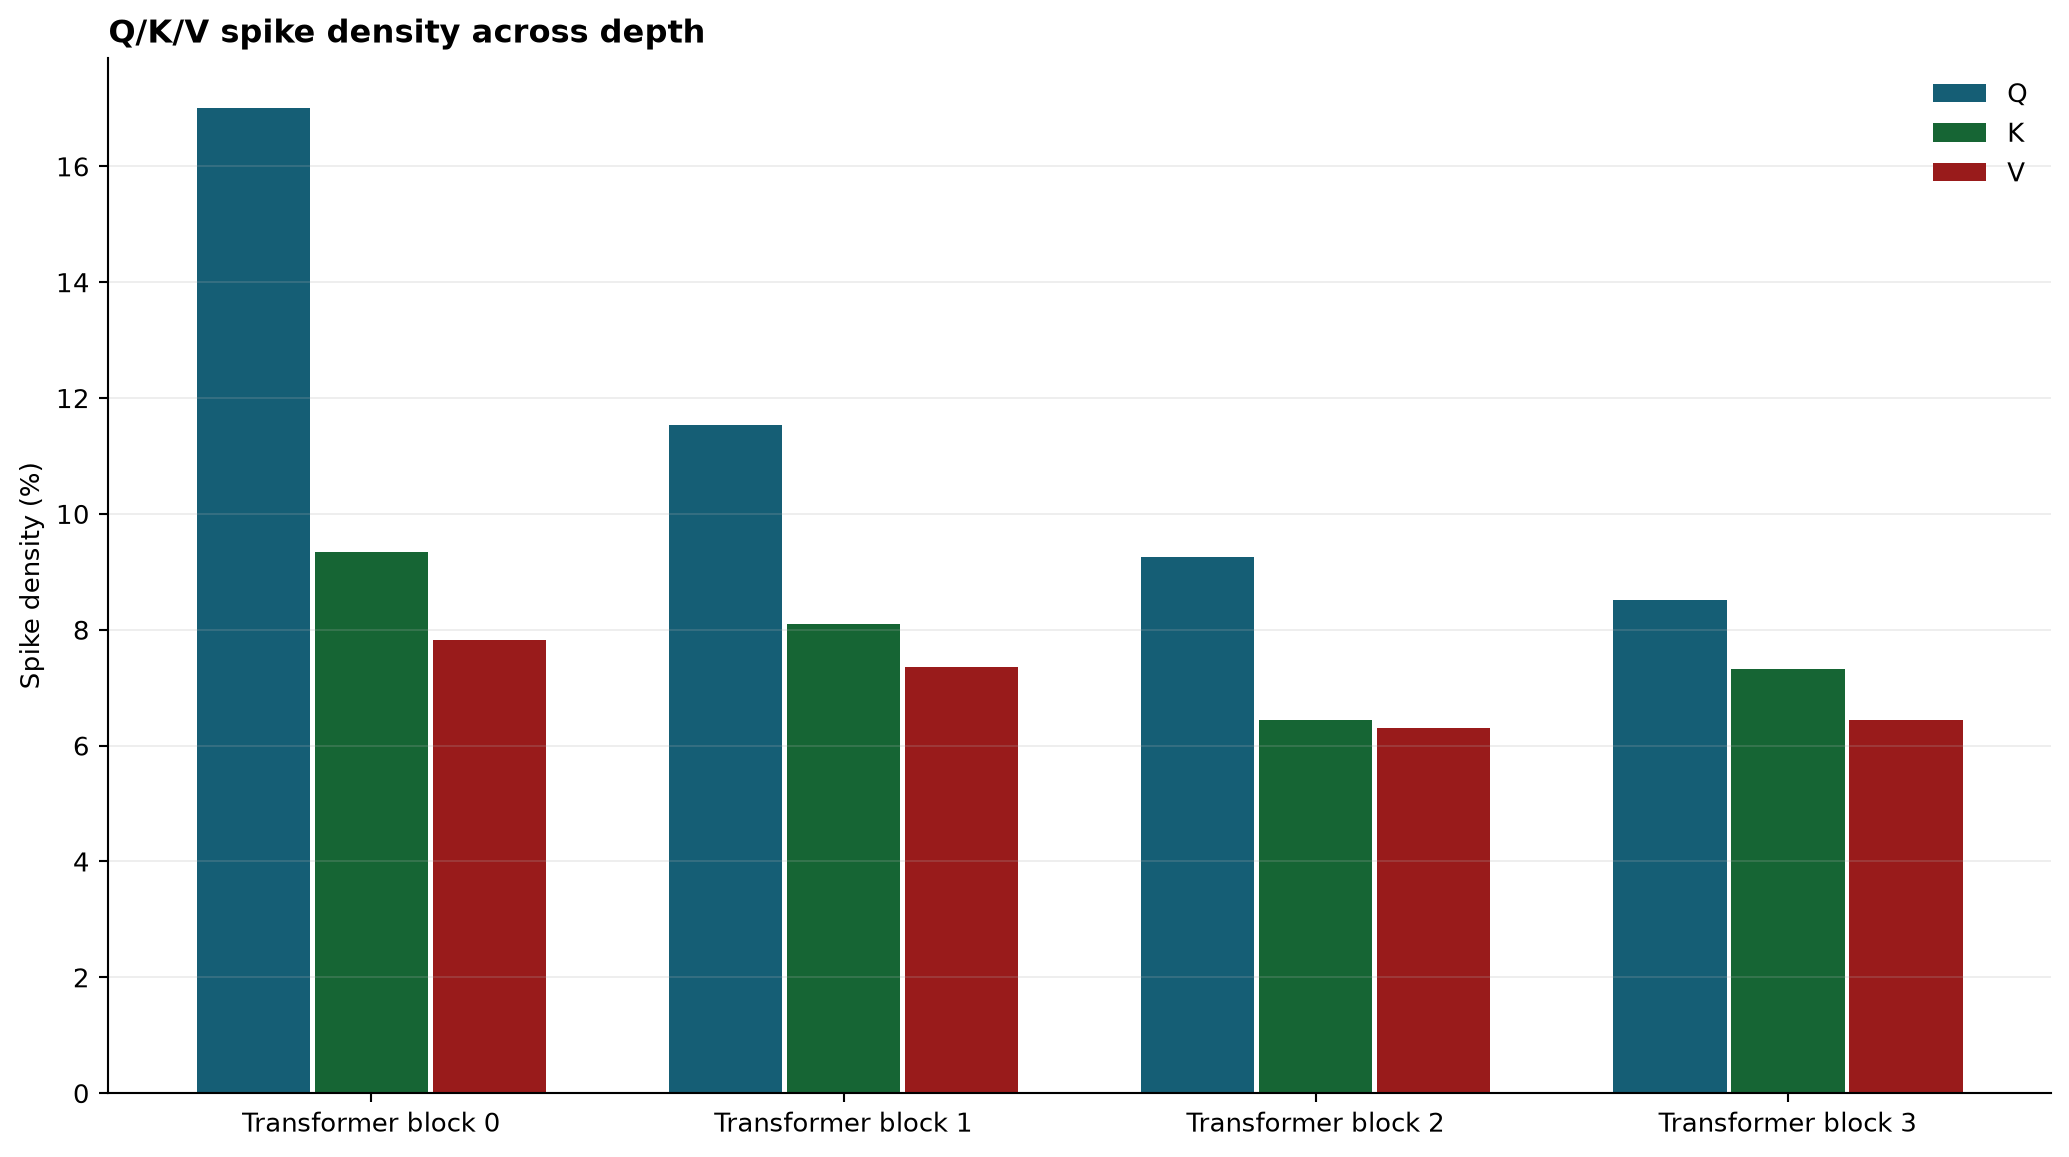
\includegraphics[width=0.98\textwidth,height=0.78\textheight,keepaspectratio]{plots/12_qkv_density.png}
\end{center}
\clearpage
\section{Activation mean and spread}
\begin{sloppypar}\small\textbf{Evidence:} full-test streaming activation moments\end{sloppypar}
\begin{center}
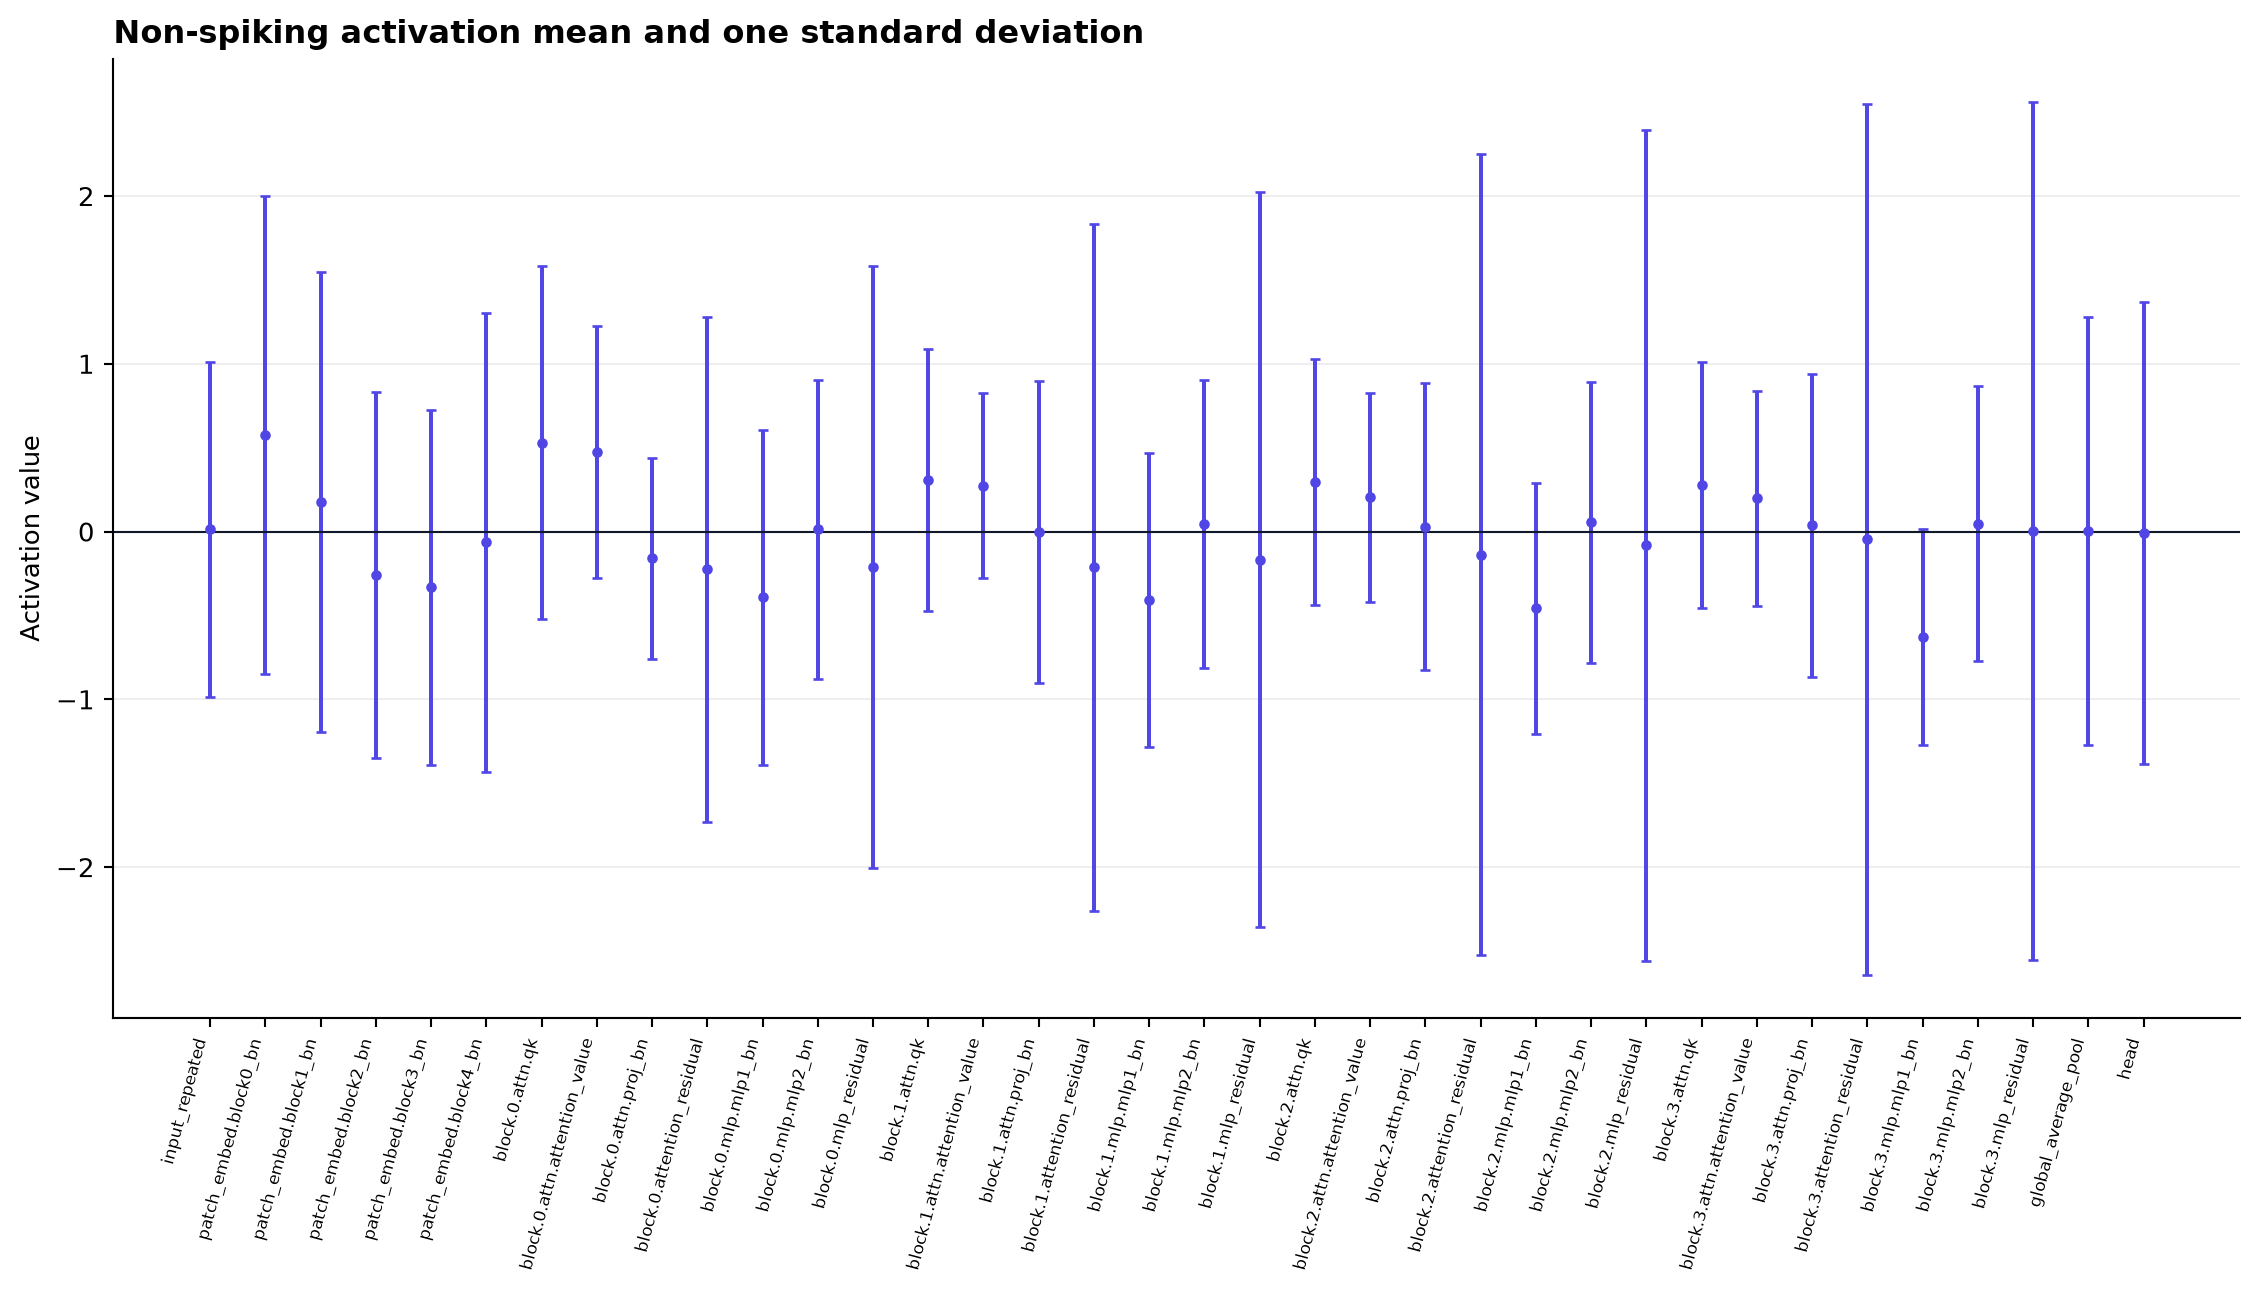
\includegraphics[width=0.98\textwidth,height=0.78\textheight,keepaspectratio]{plots/13_activation_moments.png}
\end{center}
\clearpage
\section{Model work by learned operator}
\begin{sloppypar}\small\textbf{Evidence:} execution manifest generated from exported tensor shapes\end{sloppypar}
\begin{center}
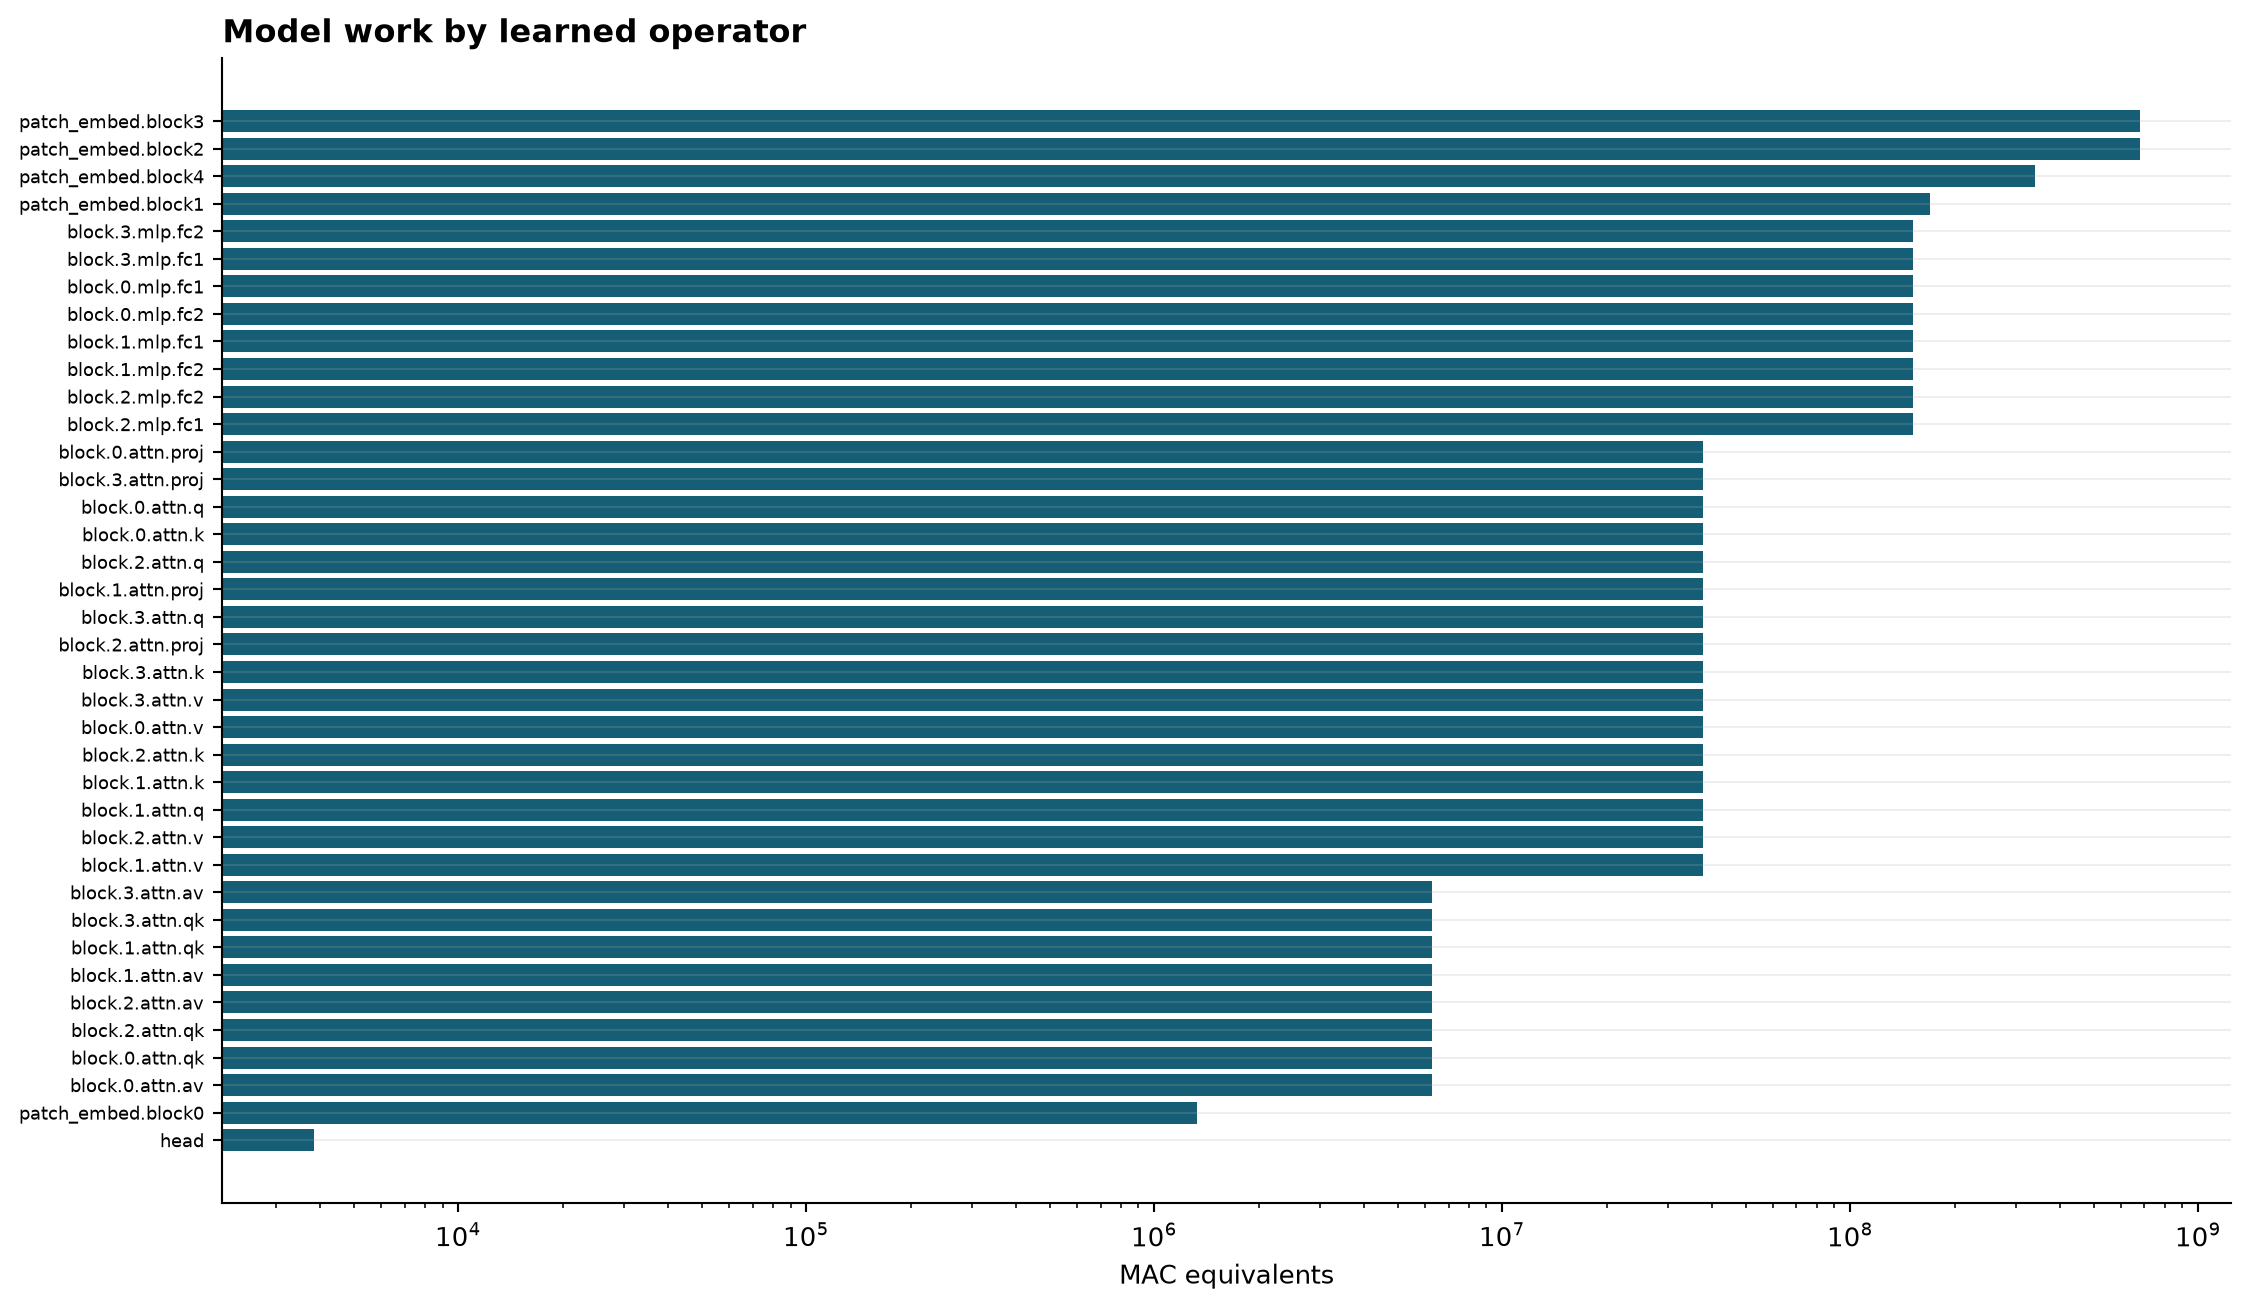
\includegraphics[width=0.98\textwidth,height=0.78\textheight,keepaspectratio]{plots/14_operator_macs.png}
\end{center}
\clearpage
\section{Tile commands by learned operator}
\begin{sloppypar}\small\textbf{Evidence:} execution manifest generated from exported tensor shapes\end{sloppypar}
\begin{center}
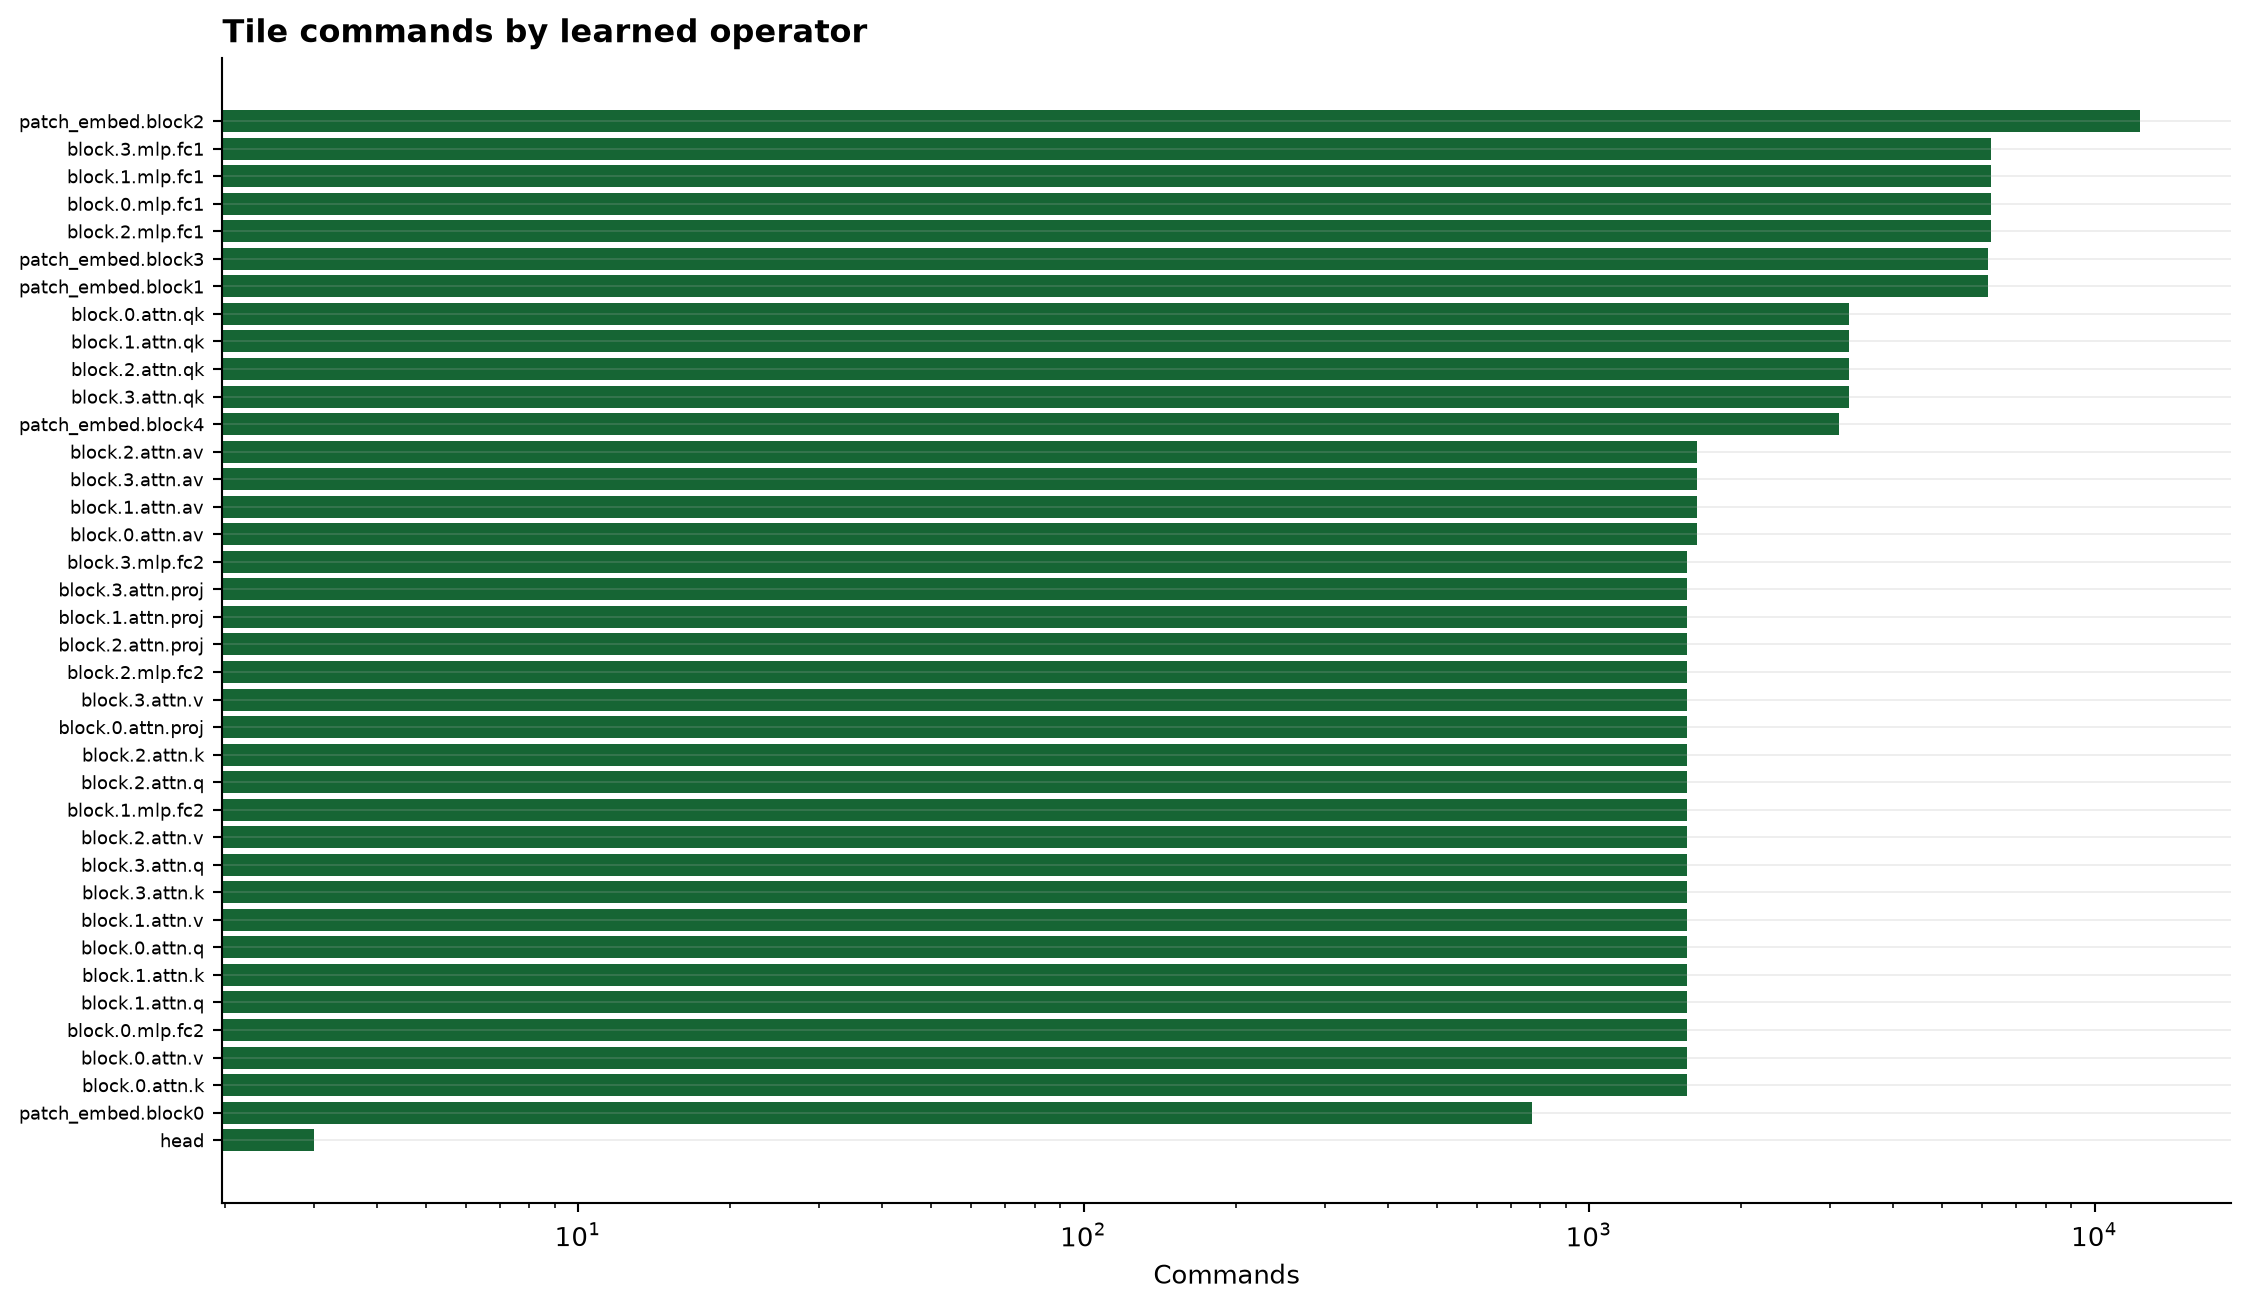
\includegraphics[width=0.98\textwidth,height=0.78\textheight,keepaspectratio]{plots/15_operator_commands.png}
\end{center}
\clearpage
\section{Operator stream traffic}
\begin{sloppypar}\small\textbf{Evidence:} execution manifest;\allowbreak{} excludes inter-layer DDR spill\end{sloppypar}
\begin{center}
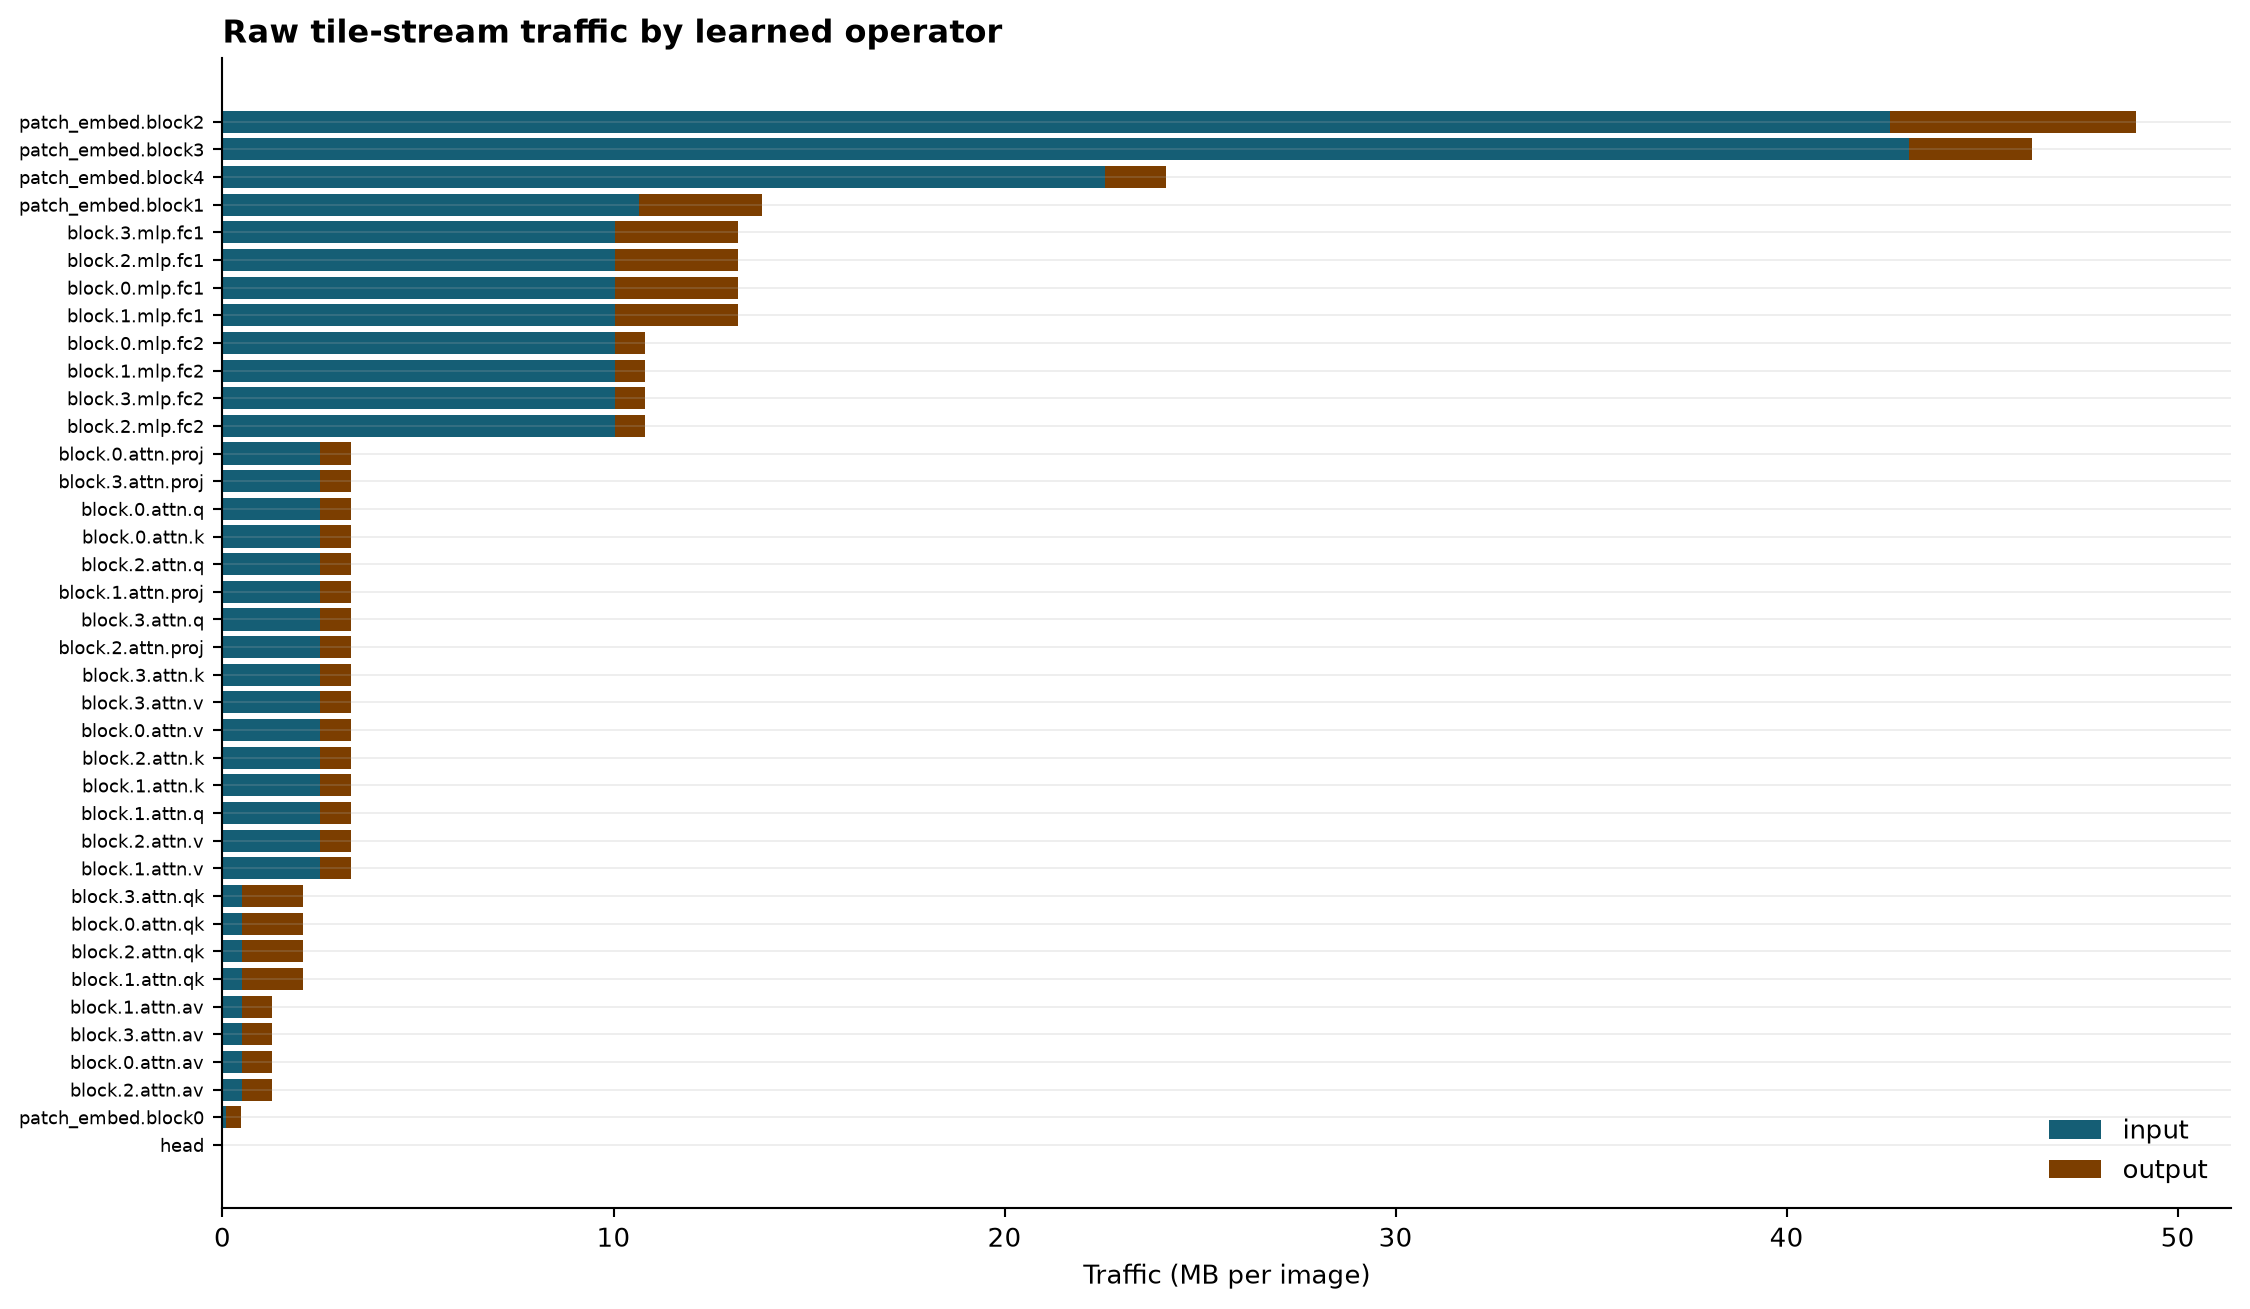
\includegraphics[width=0.98\textwidth,height=0.78\textheight,keepaspectratio]{plots/16_operator_traffic.png}
\end{center}
\clearpage
\section{Arithmetic mode share}
\begin{sloppypar}\small\textbf{Evidence:} execution manifest model-equivalent operation counts\end{sloppypar}
\begin{center}
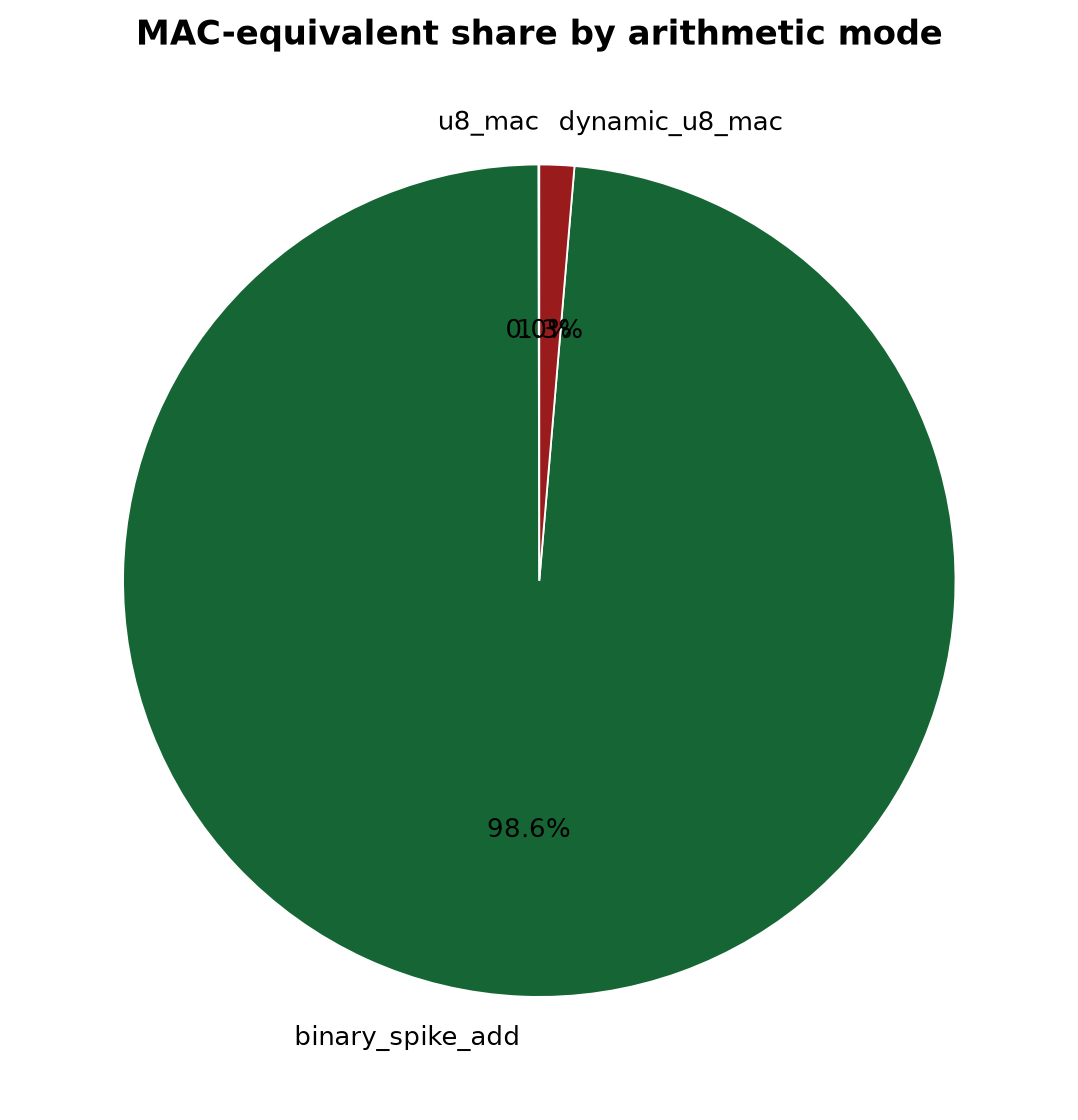
\includegraphics[width=0.98\textwidth,height=0.78\textheight,keepaspectratio]{plots/17_arithmetic_share.png}
\end{center}
\clearpage
\section{Matrix shape landscape}
\begin{sloppypar}\small\textbf{Evidence:} execution manifest;\allowbreak{} marker area tracks output-row count\end{sloppypar}
\begin{center}
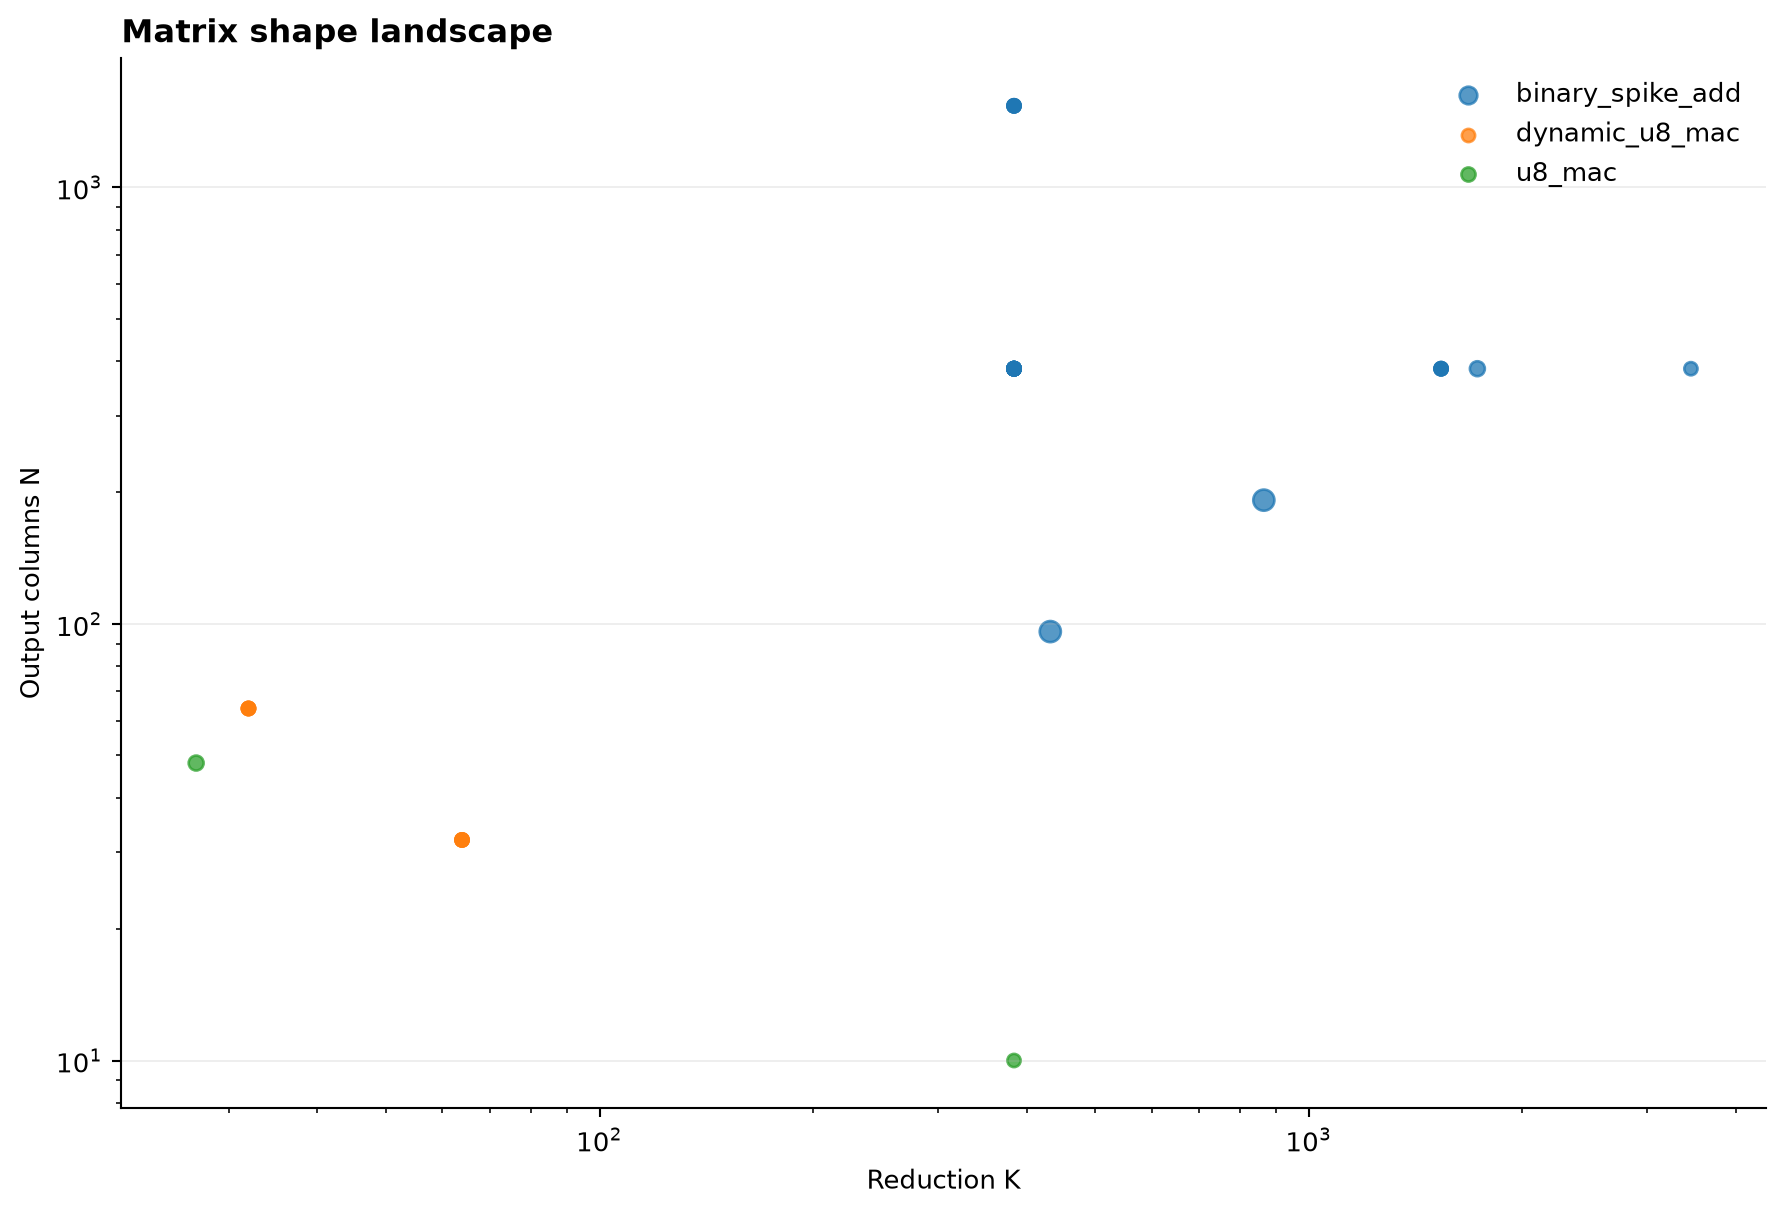
\includegraphics[width=0.98\textwidth,height=0.78\textheight,keepaspectratio]{plots/18_matrix_shapes.png}
\end{center}
\clearpage
\section{Projection quantization diagnostics}
\begin{sloppypar}\small\textbf{Evidence:} hashed hardware parameter manifest\end{sloppypar}
\begin{center}
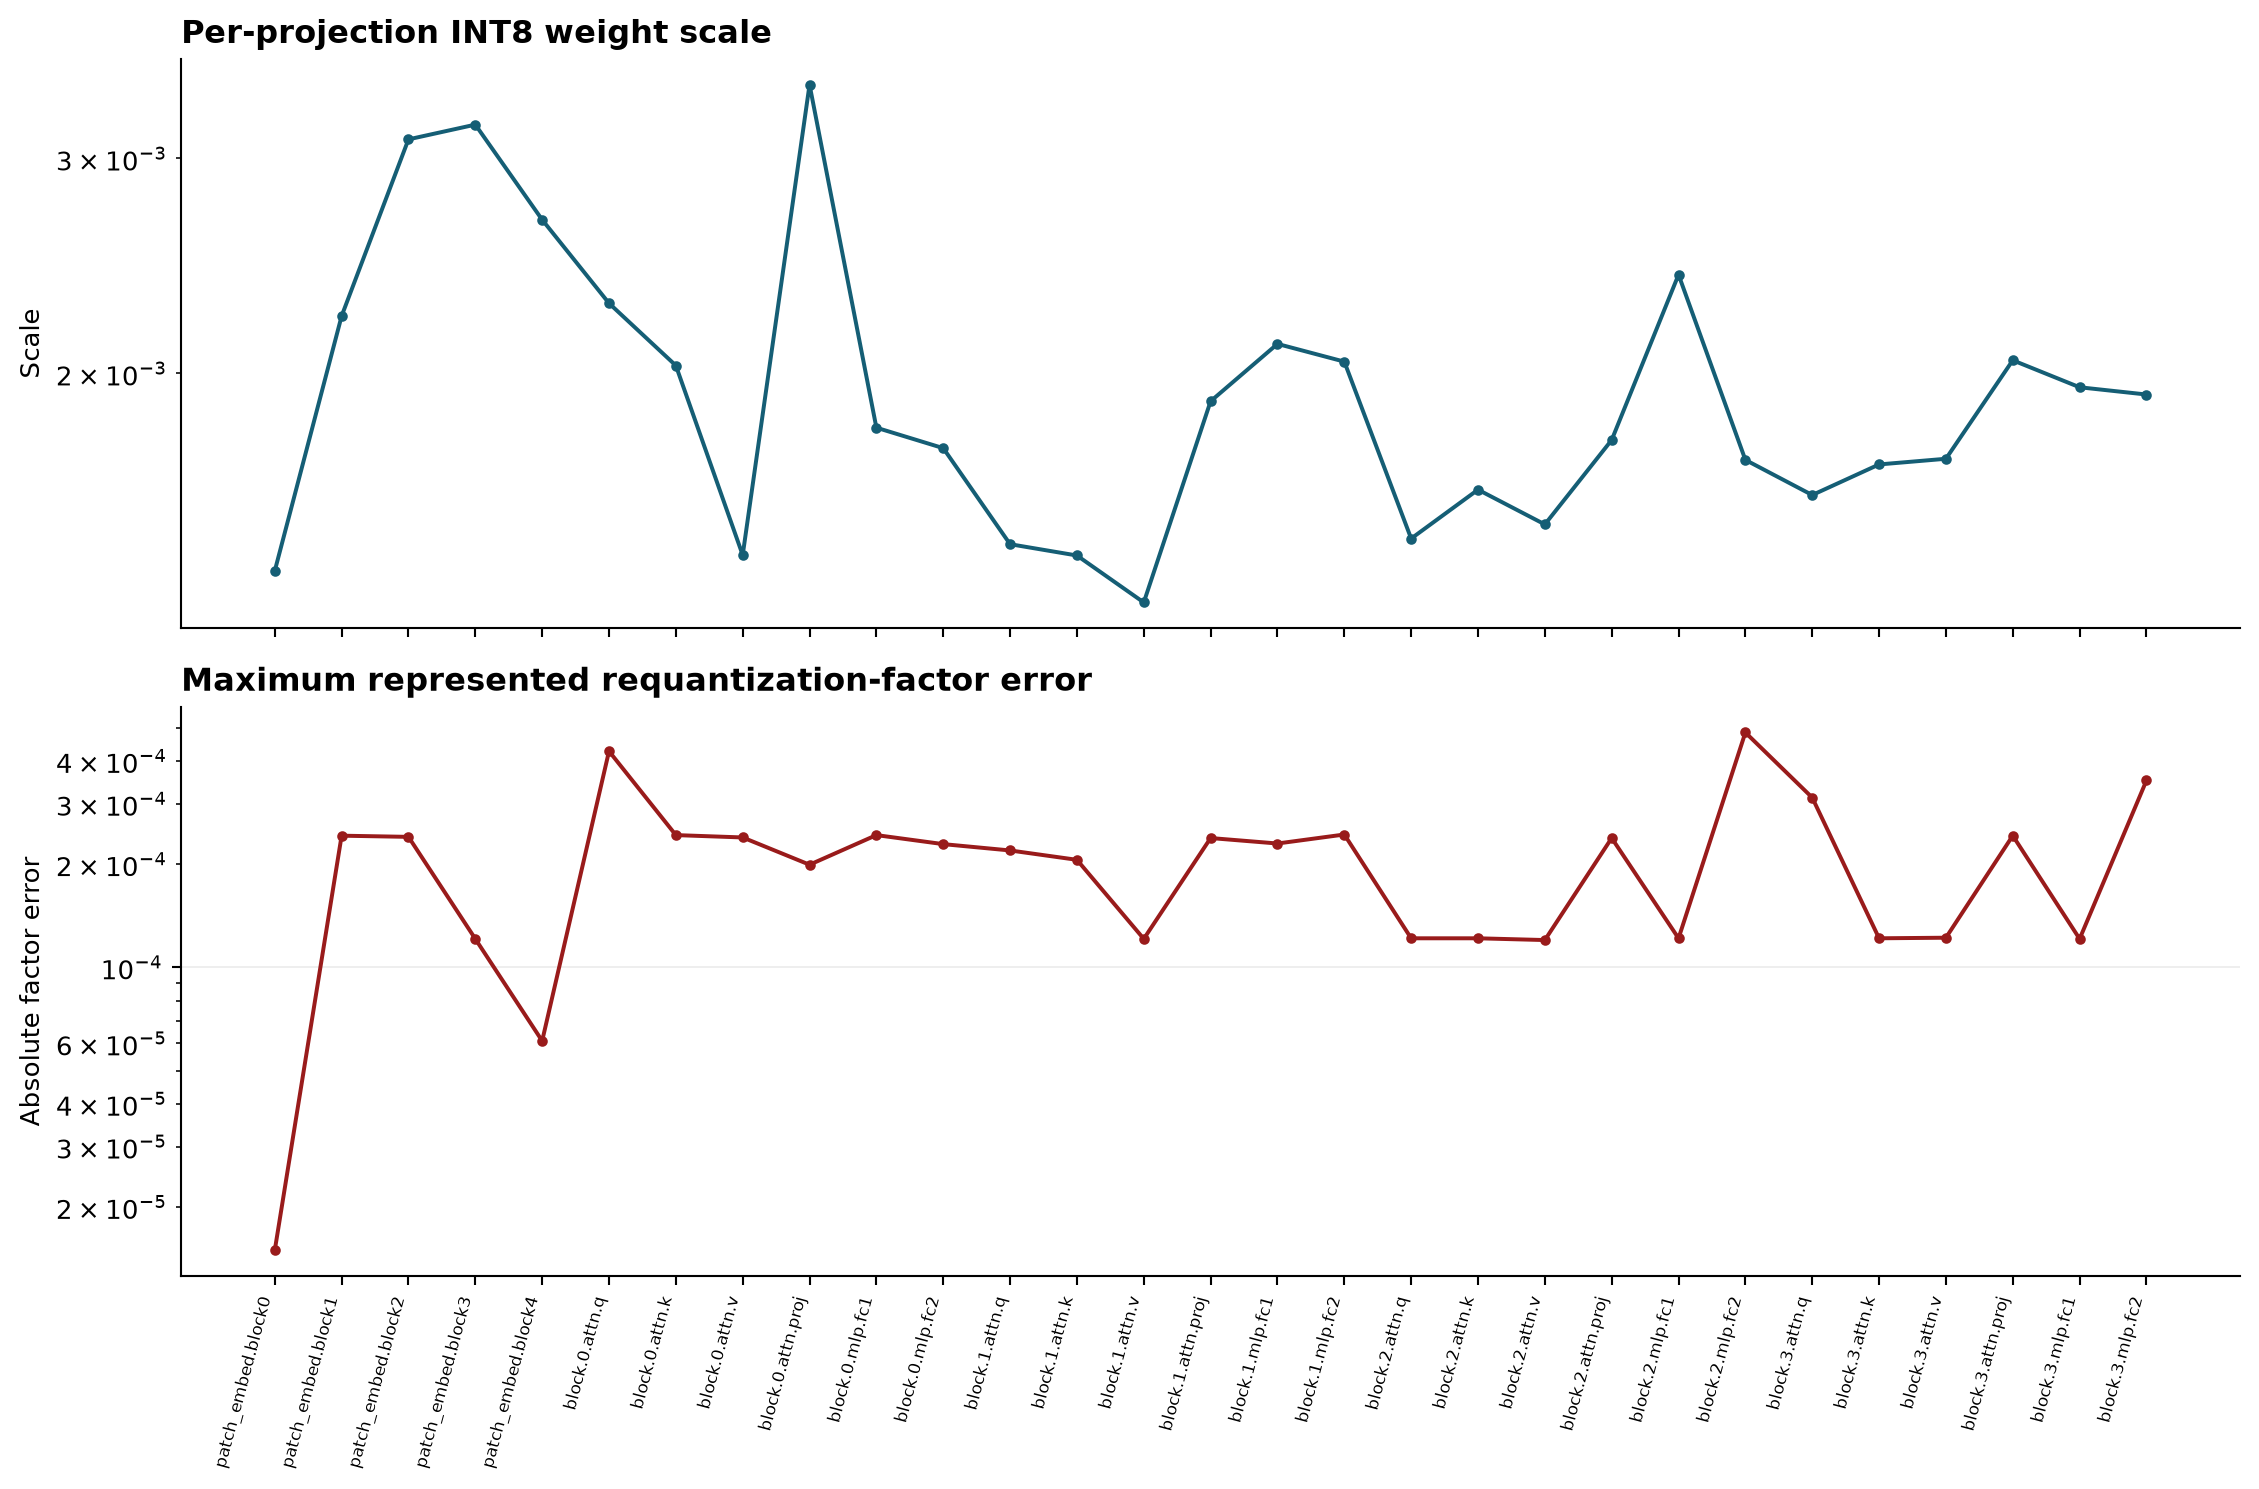
\includegraphics[width=0.98\textwidth,height=0.78\textheight,keepaspectratio]{plots/19_projection_quantization.png}
\end{center}
\clearpage
\section{Exported weight distribution}
\begin{sloppypar}\small\textbf{Evidence:} direct section views from the SHA-256-checked parameter binary\end{sloppypar}
\begin{center}
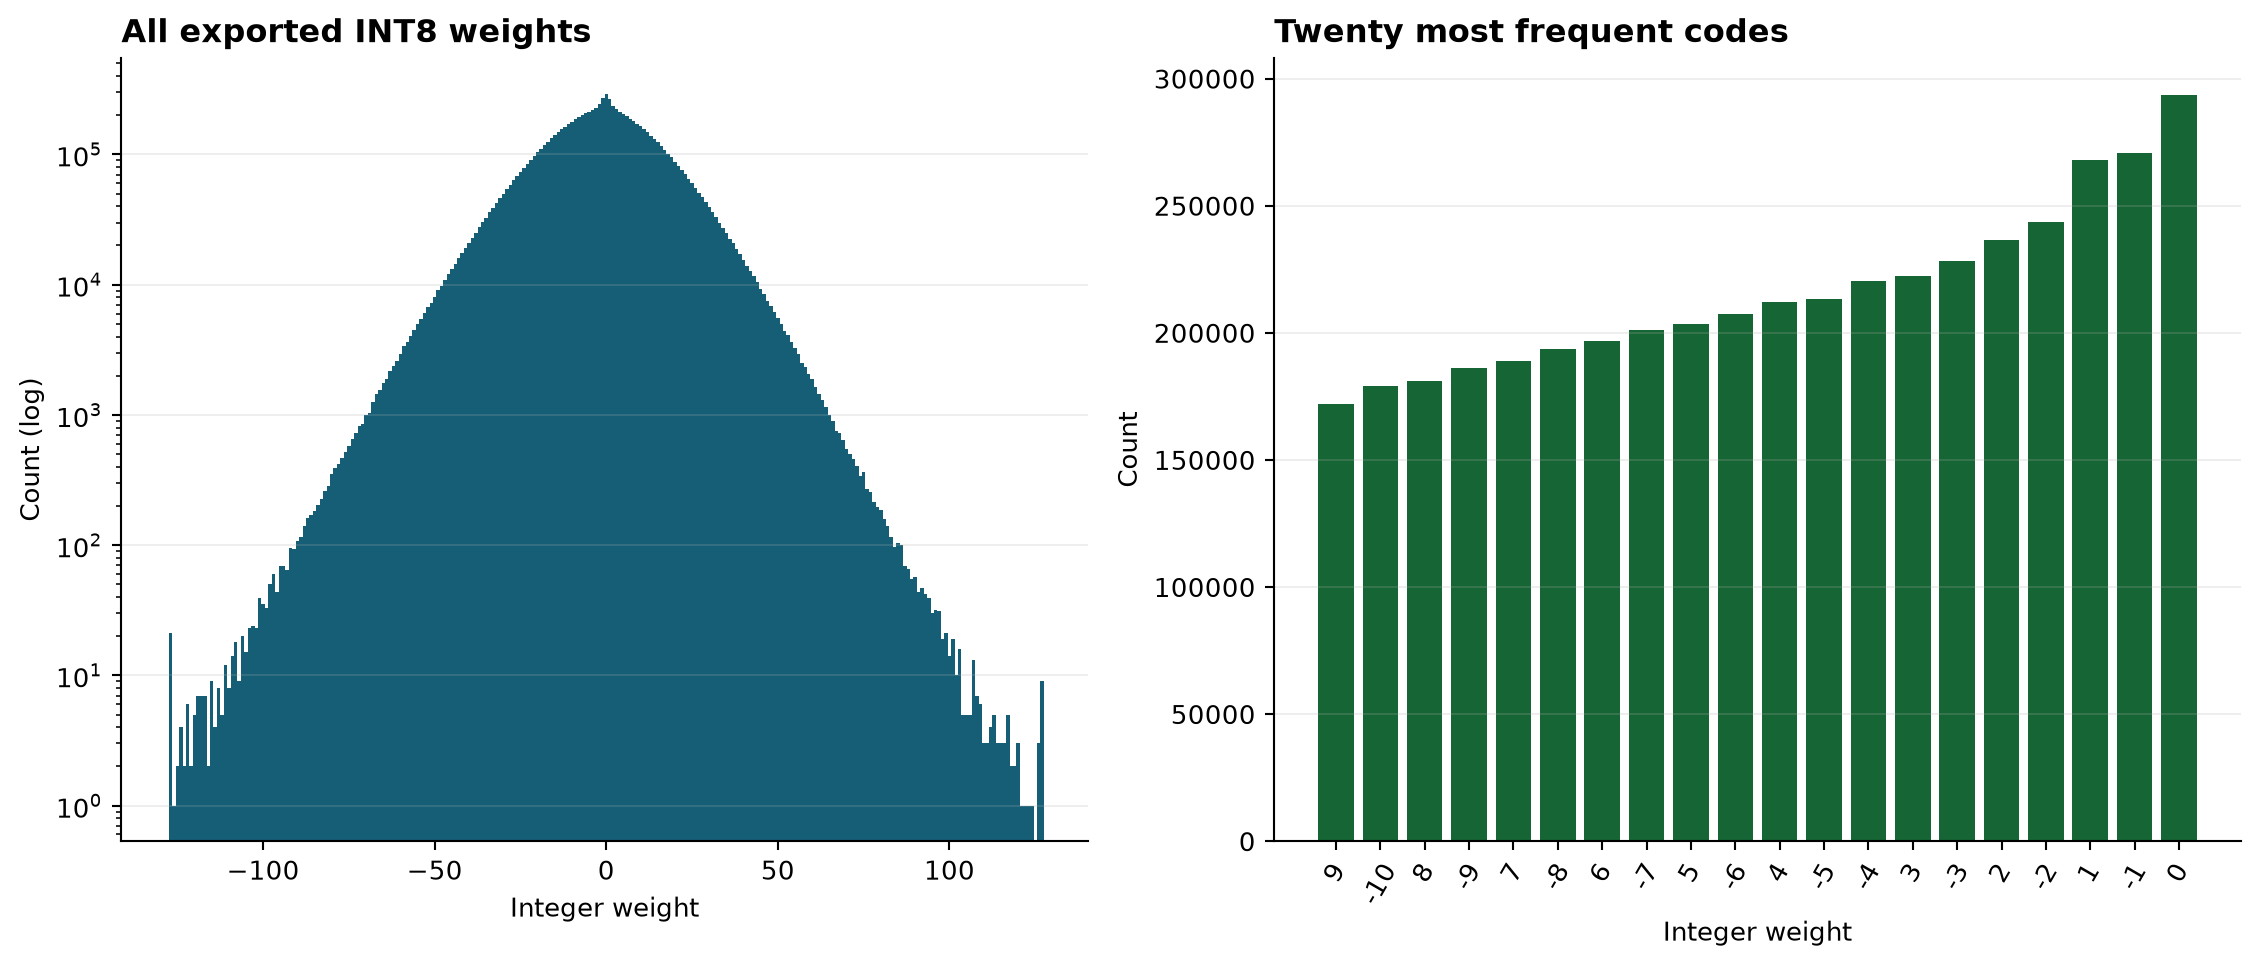
\includegraphics[width=0.98\textwidth,height=0.78\textheight,keepaspectratio]{plots/20_weight_distribution.png}
\end{center}
\clearpage
\section{Largest-layer compiler benchmark}
\begin{sloppypar}\small\textbf{Evidence:} recorded scalar baseline and outputs/\allowbreak{}benchmarks/\allowbreak{}compiler\_\allowbreak{}block3\_\allowbreak{}memory.json\end{sloppypar}
\begin{center}
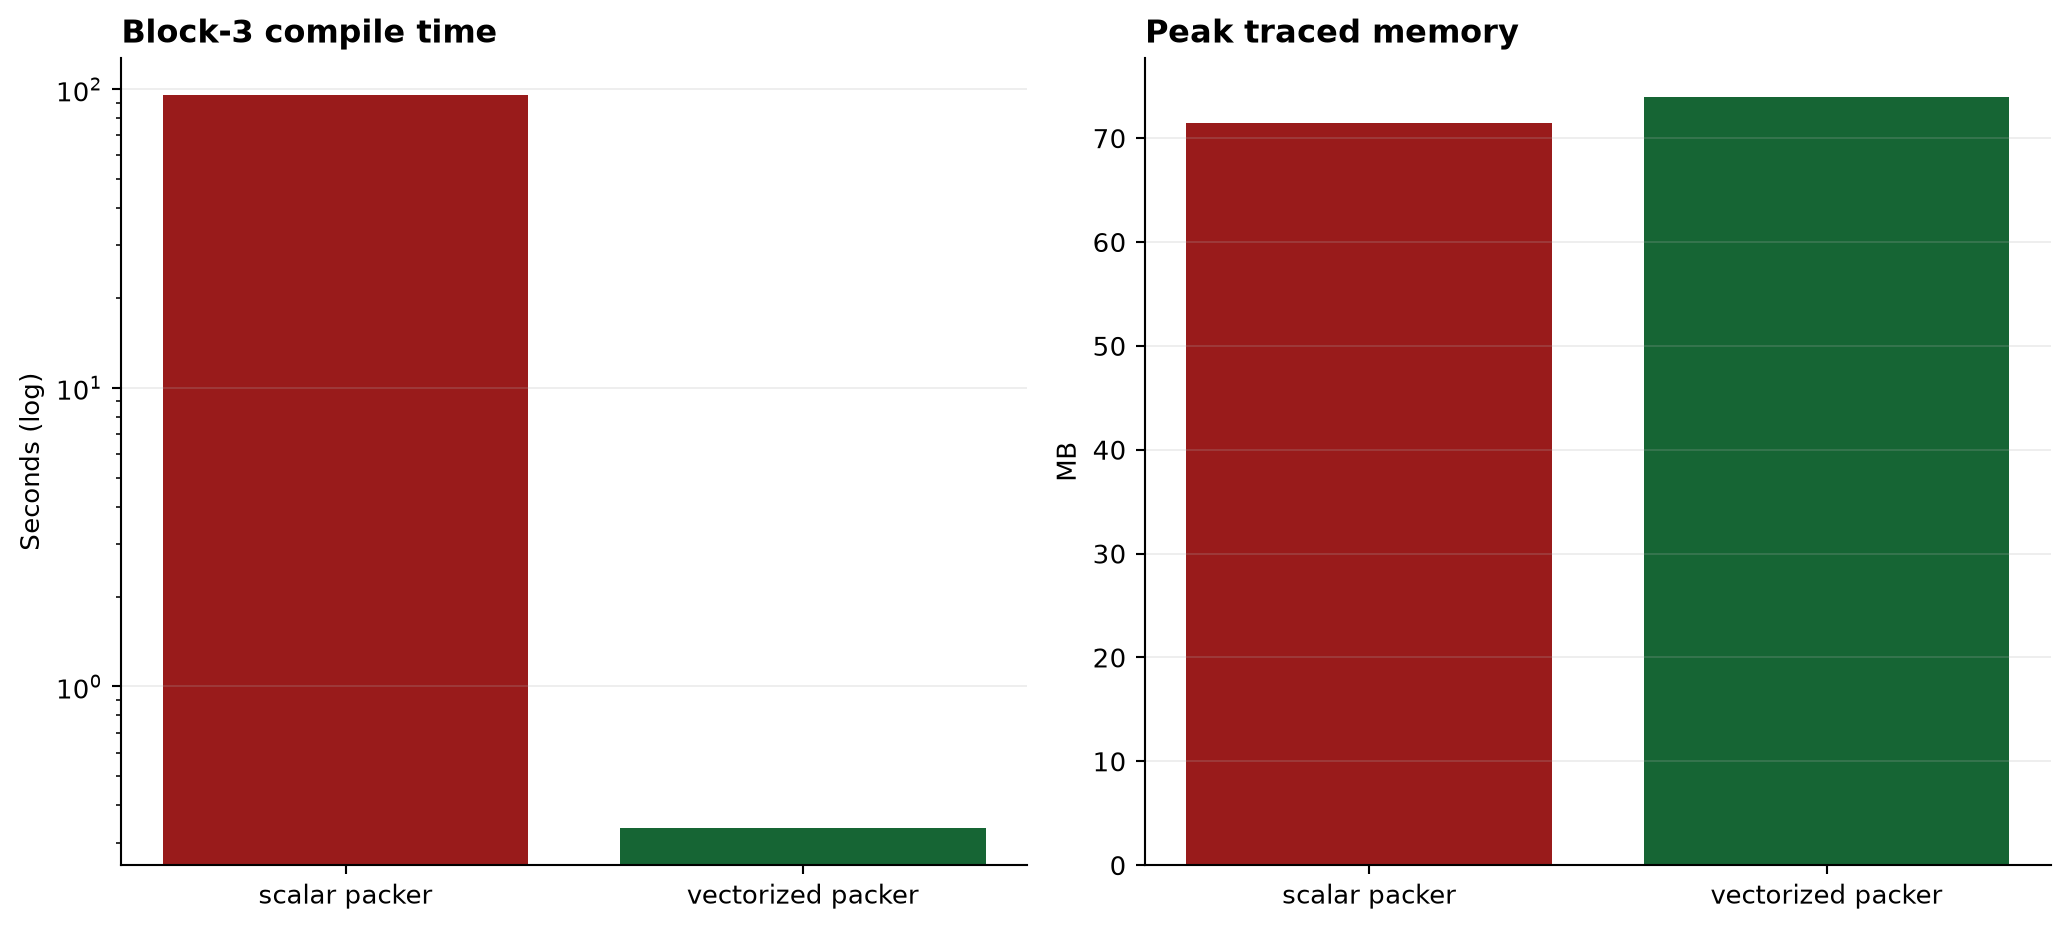
\includegraphics[width=0.98\textwidth,height=0.78\textheight,keepaspectratio]{plots/21_compiler_benchmark.png}
\end{center}
\clearpage
\section{Full-backbone training schedule and numeric contract}
\begin{sloppypar}\small\textbf{Evidence:} C:\textbackslash{}\allowbreak{}Users\textbackslash{}\allowbreak{}Ross\textbackslash{}\allowbreak{}Downloads\textbackslash{}\allowbreak{}neuraedge--main\textbackslash{}\allowbreak{}neuraedge--main\textbackslash{}\allowbreak{}neuraedge\_\allowbreak{}universal\textbackslash{}\allowbreak{}outputs\textbackslash{}\allowbreak{}training\textbackslash{}\allowbreak{}spikingformer\_\allowbreak{}training\_\allowbreak{}coverage.json\end{sloppypar}
\begin{center}
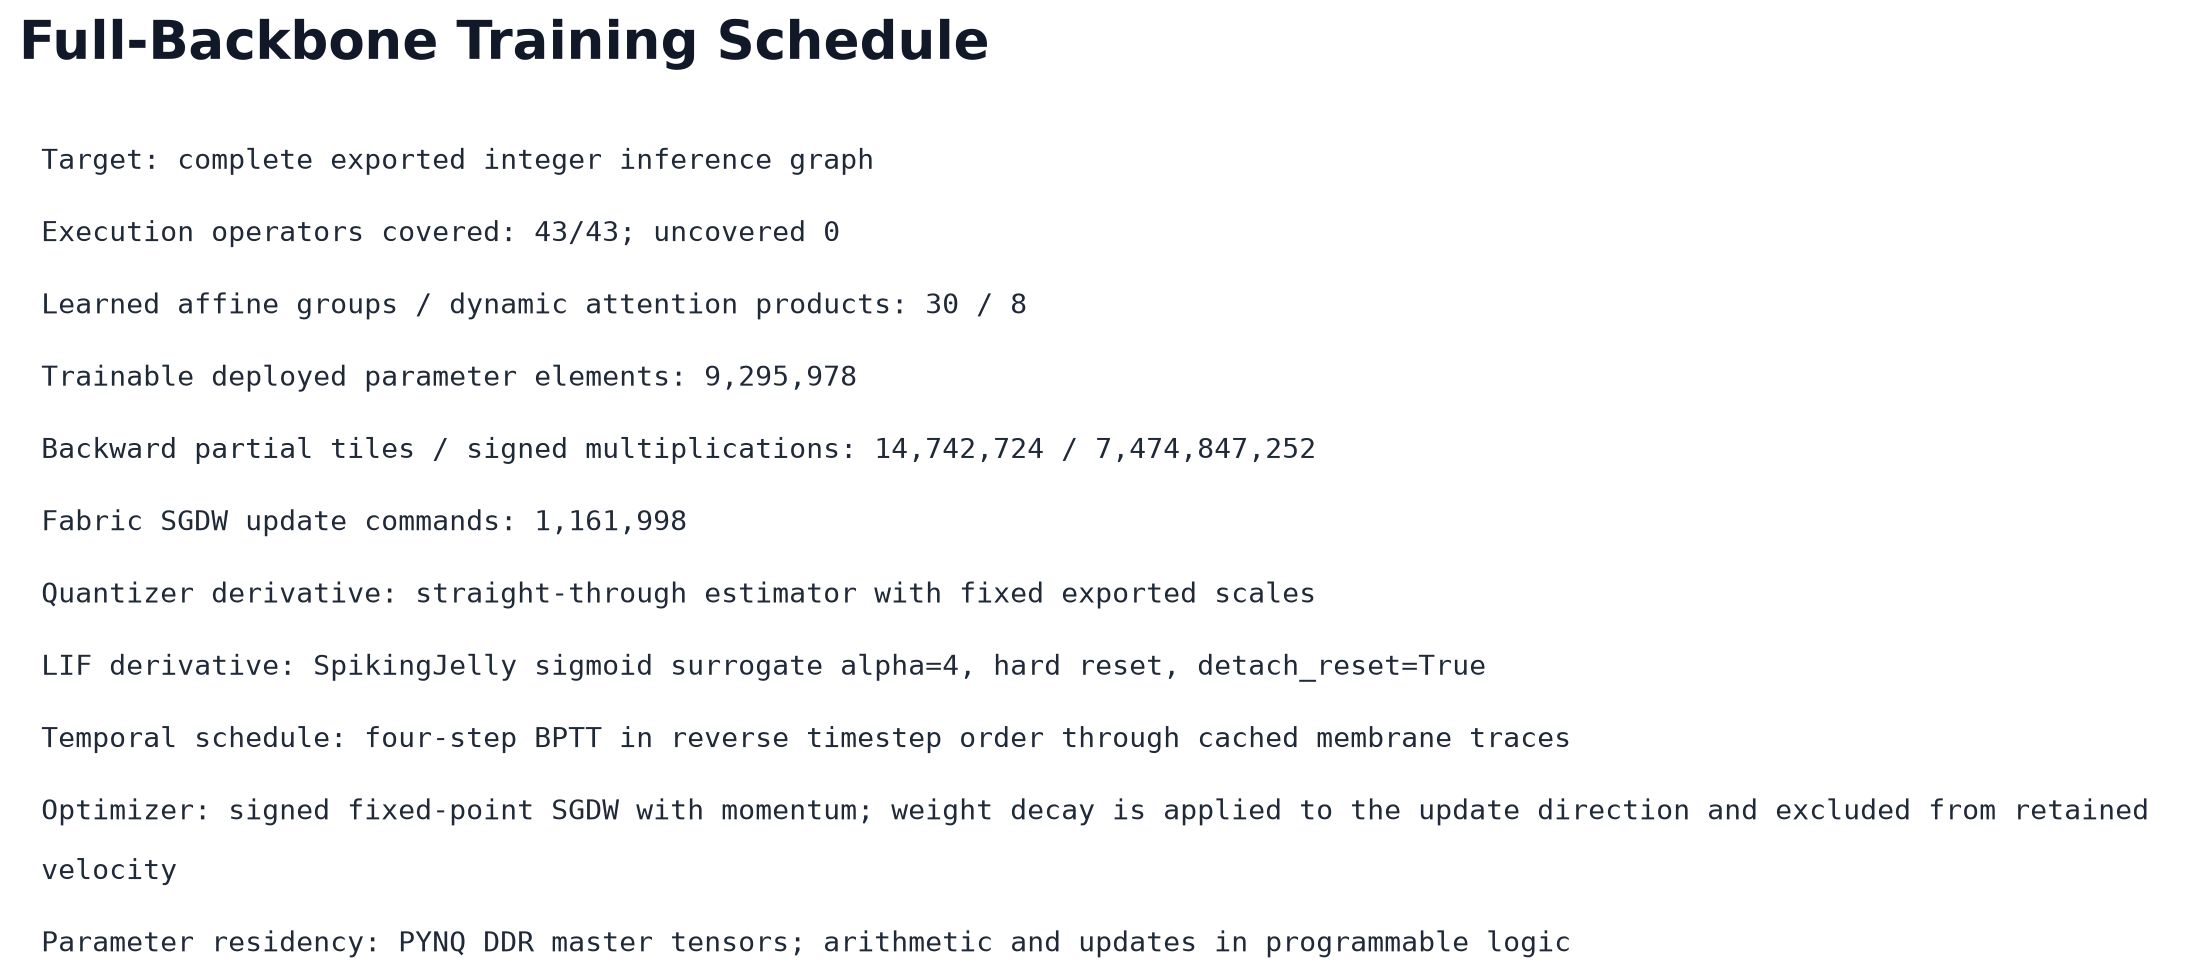
\includegraphics[width=0.98\textwidth,height=0.78\textheight,keepaspectratio]{plots/22_training_schedule.png}
\end{center}
\clearpage
\section{Trainable deployed parameter distribution}
\begin{sloppypar}\small\textbf{Evidence:} C:\textbackslash{}\allowbreak{}Users\textbackslash{}\allowbreak{}Ross\textbackslash{}\allowbreak{}Downloads\textbackslash{}\allowbreak{}neuraedge--main\textbackslash{}\allowbreak{}neuraedge--main\textbackslash{}\allowbreak{}neuraedge\_\allowbreak{}universal\textbackslash{}\allowbreak{}outputs\textbackslash{}\allowbreak{}training\textbackslash{}\allowbreak{}spikingformer\_\allowbreak{}training\_\allowbreak{}coverage.json\end{sloppypar}
\begin{center}
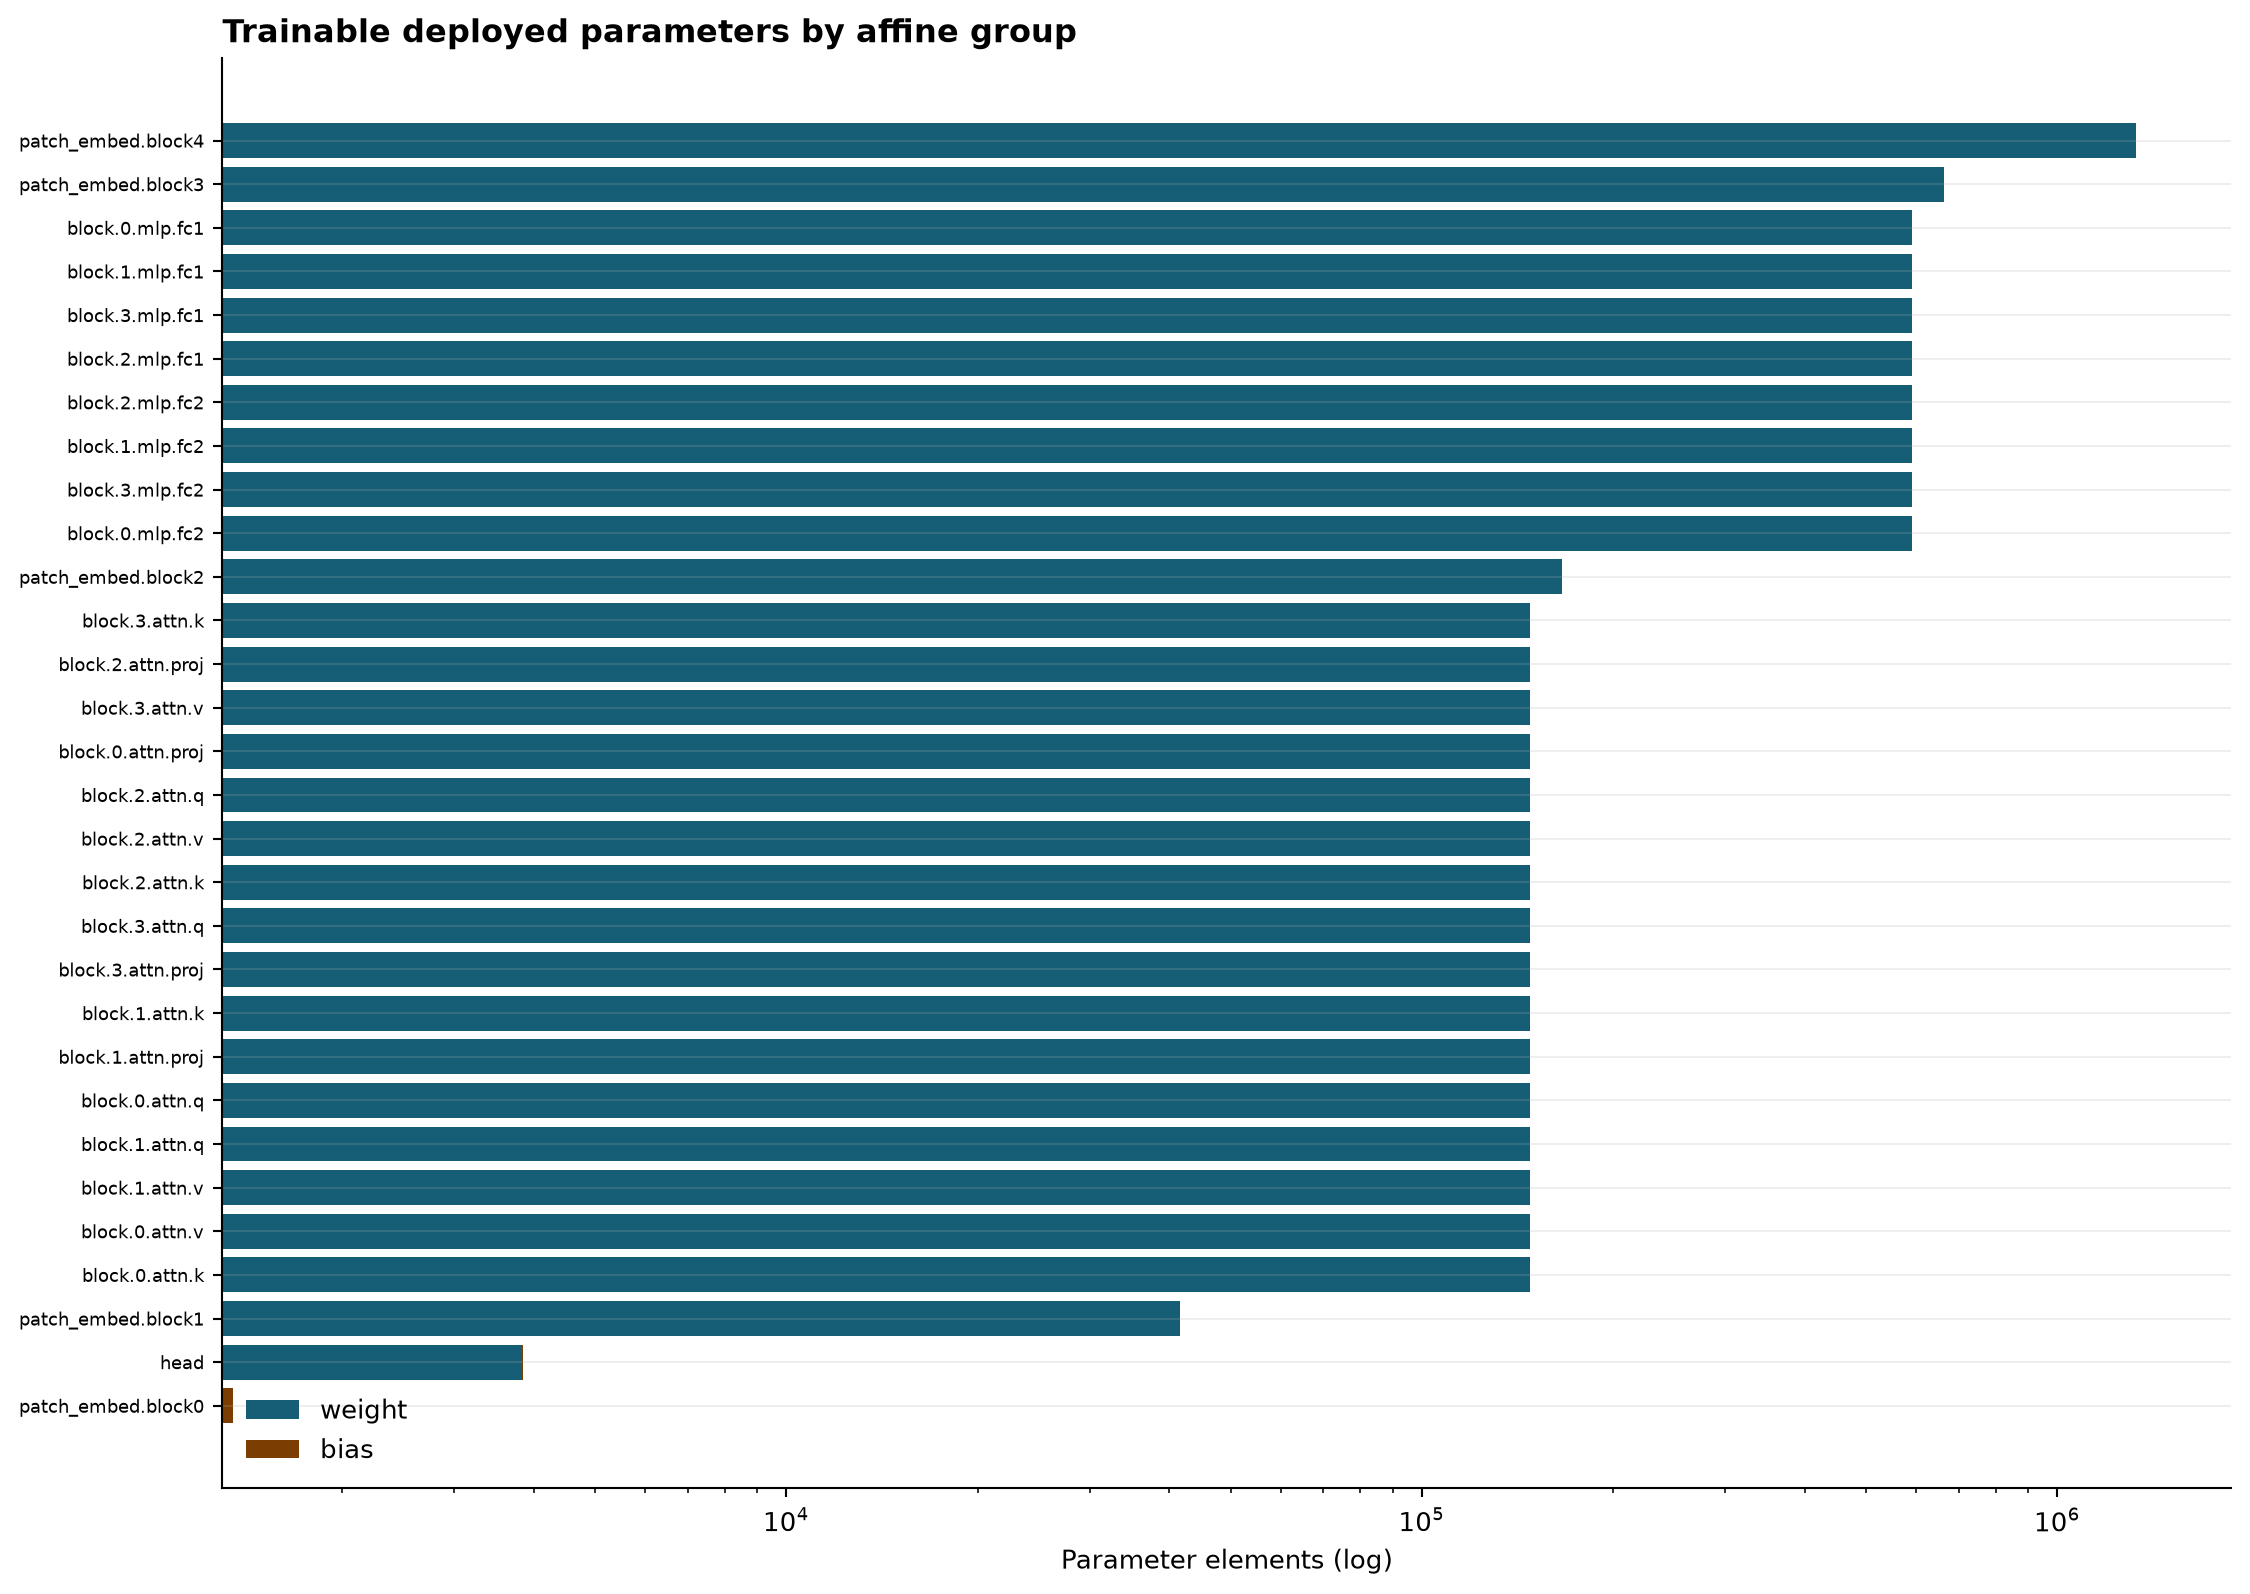
\includegraphics[width=0.98\textwidth,height=0.78\textheight,keepaspectratio]{plots/23_training_parameters.png}
\end{center}
\clearpage
\section{Exact learned-layer backward work}
\begin{sloppypar}\small\textbf{Evidence:} C:\textbackslash{}\allowbreak{}Users\textbackslash{}\allowbreak{}Ross\textbackslash{}\allowbreak{}Downloads\textbackslash{}\allowbreak{}neuraedge--main\textbackslash{}\allowbreak{}neuraedge--main\textbackslash{}\allowbreak{}neuraedge\_\allowbreak{}universal\textbackslash{}\allowbreak{}outputs\textbackslash{}\allowbreak{}training\textbackslash{}\allowbreak{}spikingformer\_\allowbreak{}training\_\allowbreak{}coverage.json\end{sloppypar}
\begin{center}
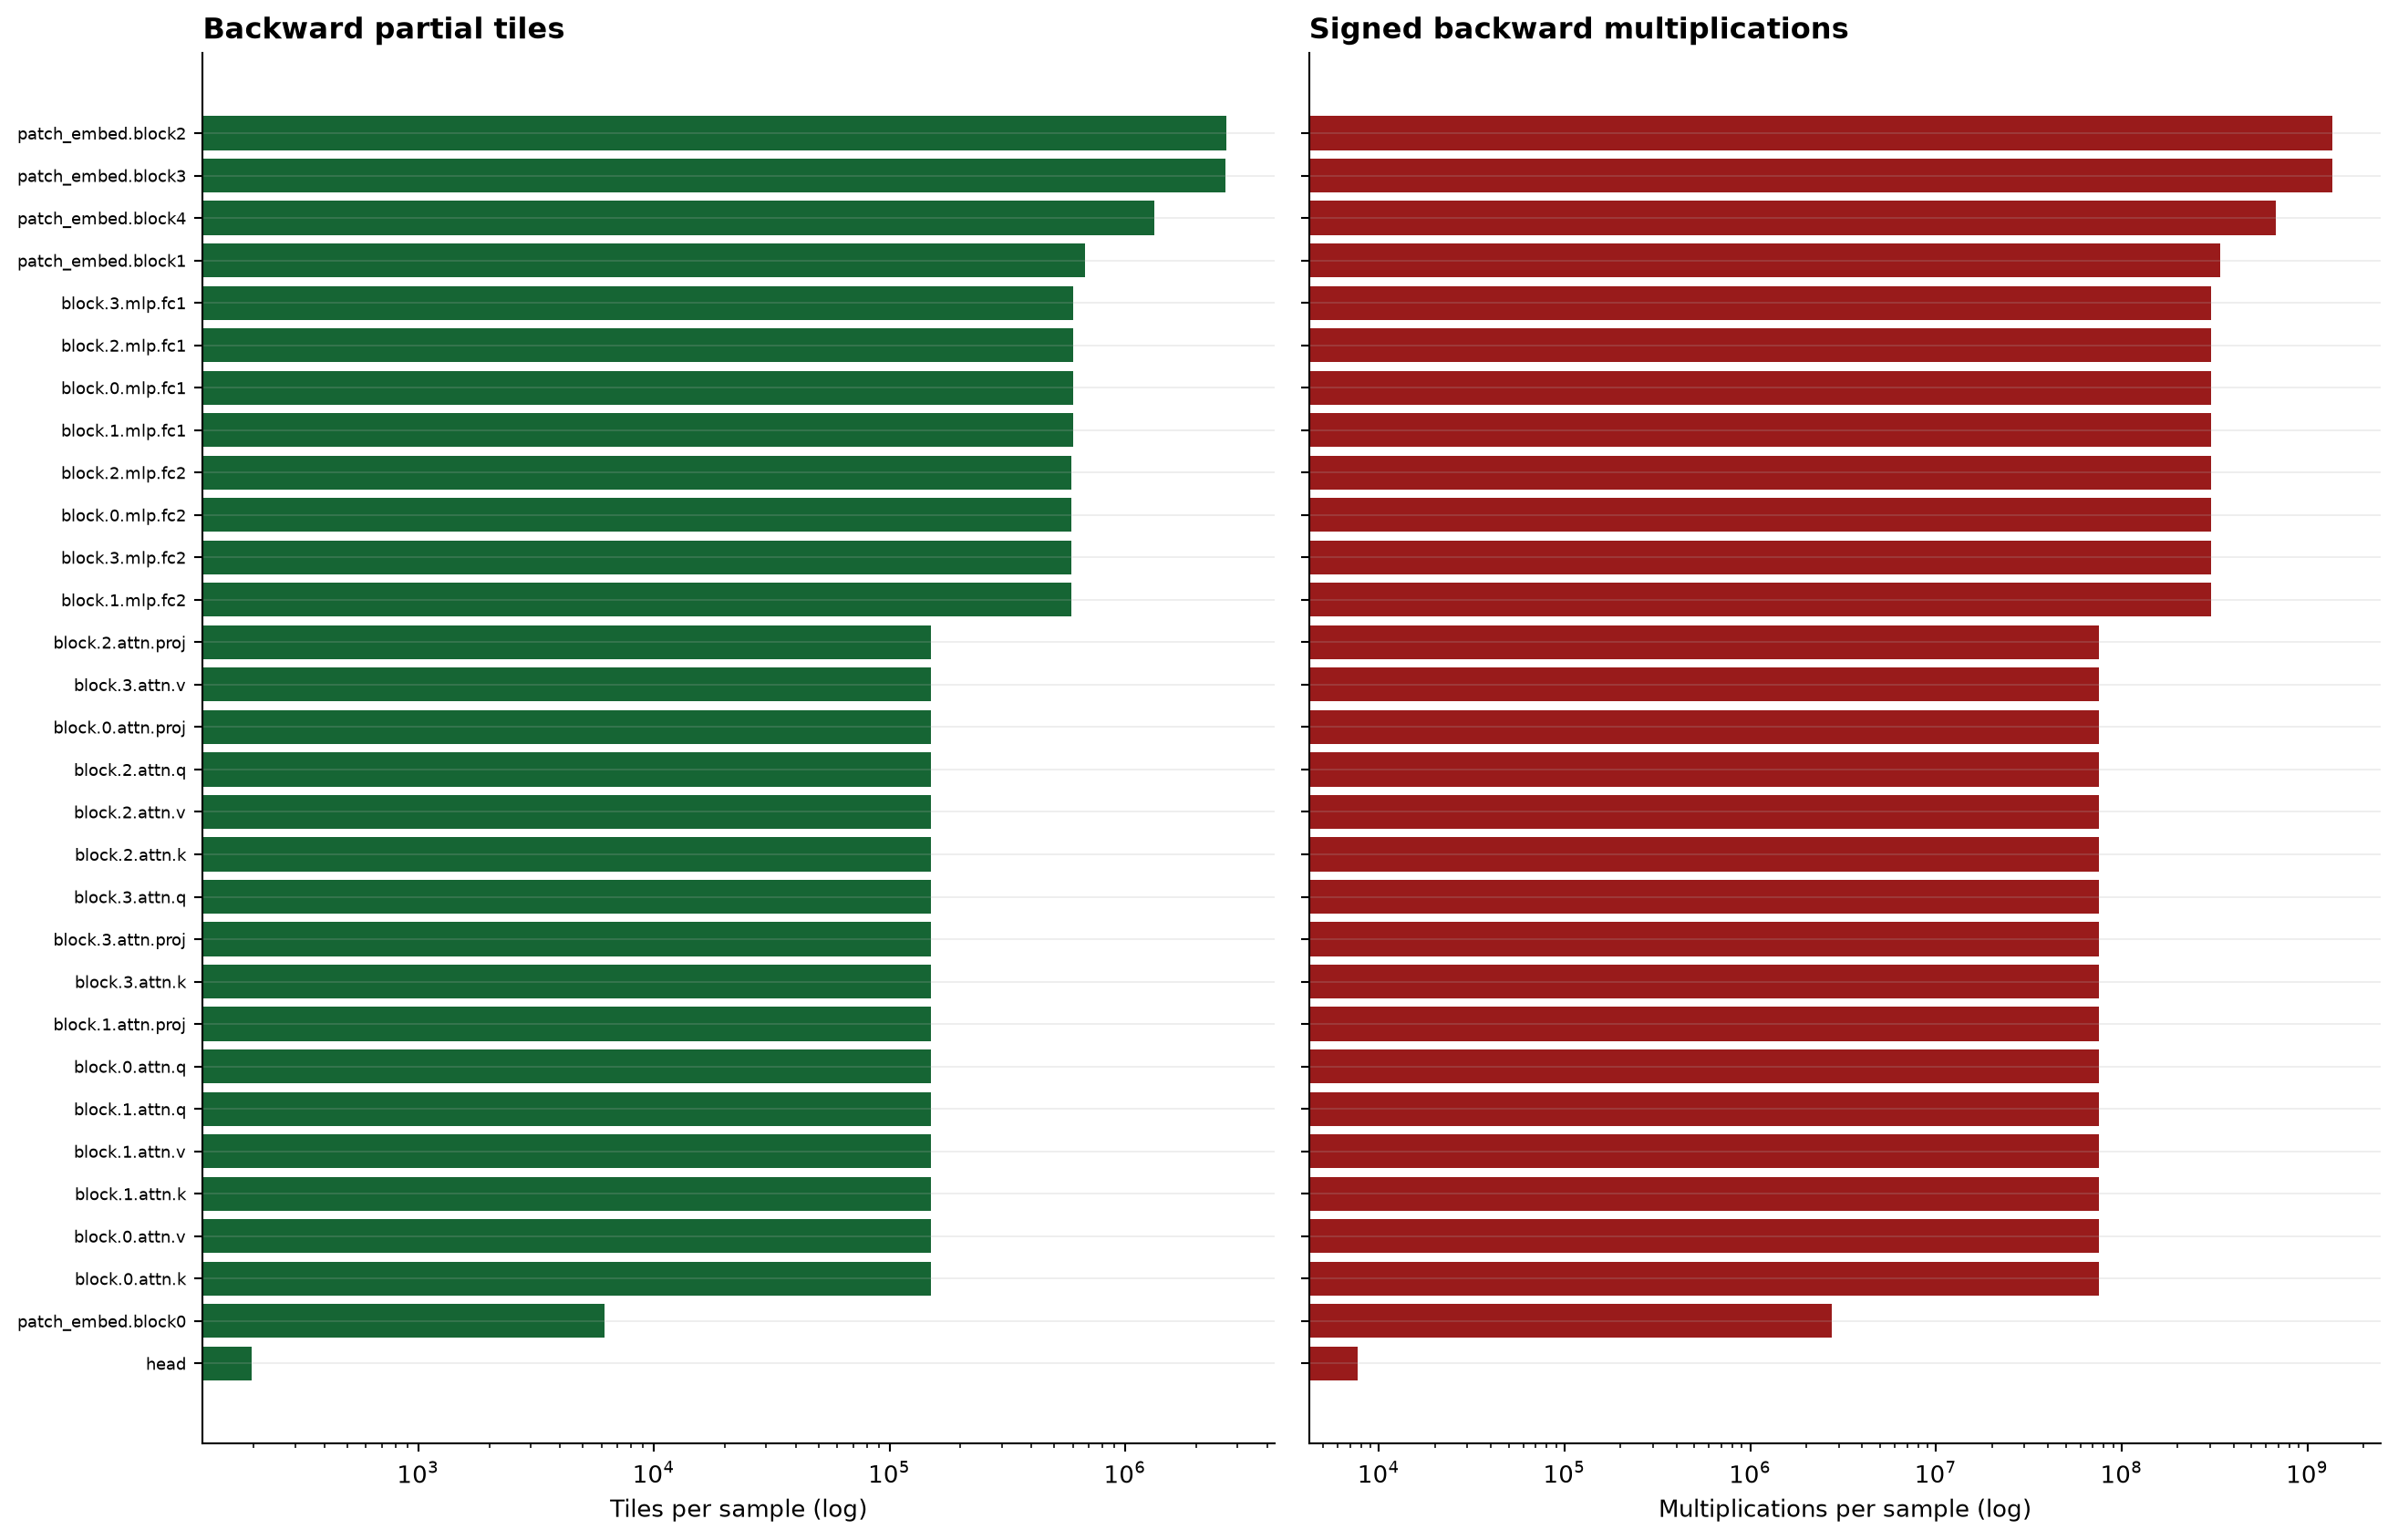
\includegraphics[width=0.98\textwidth,height=0.78\textheight,keepaspectratio]{plots/24_training_backward_work.png}
\end{center}
\clearpage
\section{Backward operator coverage and work composition}
\begin{sloppypar}\small\textbf{Evidence:} C:\textbackslash{}\allowbreak{}Users\textbackslash{}\allowbreak{}Ross\textbackslash{}\allowbreak{}Downloads\textbackslash{}\allowbreak{}neuraedge--main\textbackslash{}\allowbreak{}neuraedge--main\textbackslash{}\allowbreak{}neuraedge\_\allowbreak{}universal\textbackslash{}\allowbreak{}outputs\textbackslash{}\allowbreak{}training\textbackslash{}\allowbreak{}spikingformer\_\allowbreak{}training\_\allowbreak{}coverage.json\end{sloppypar}
\begin{center}
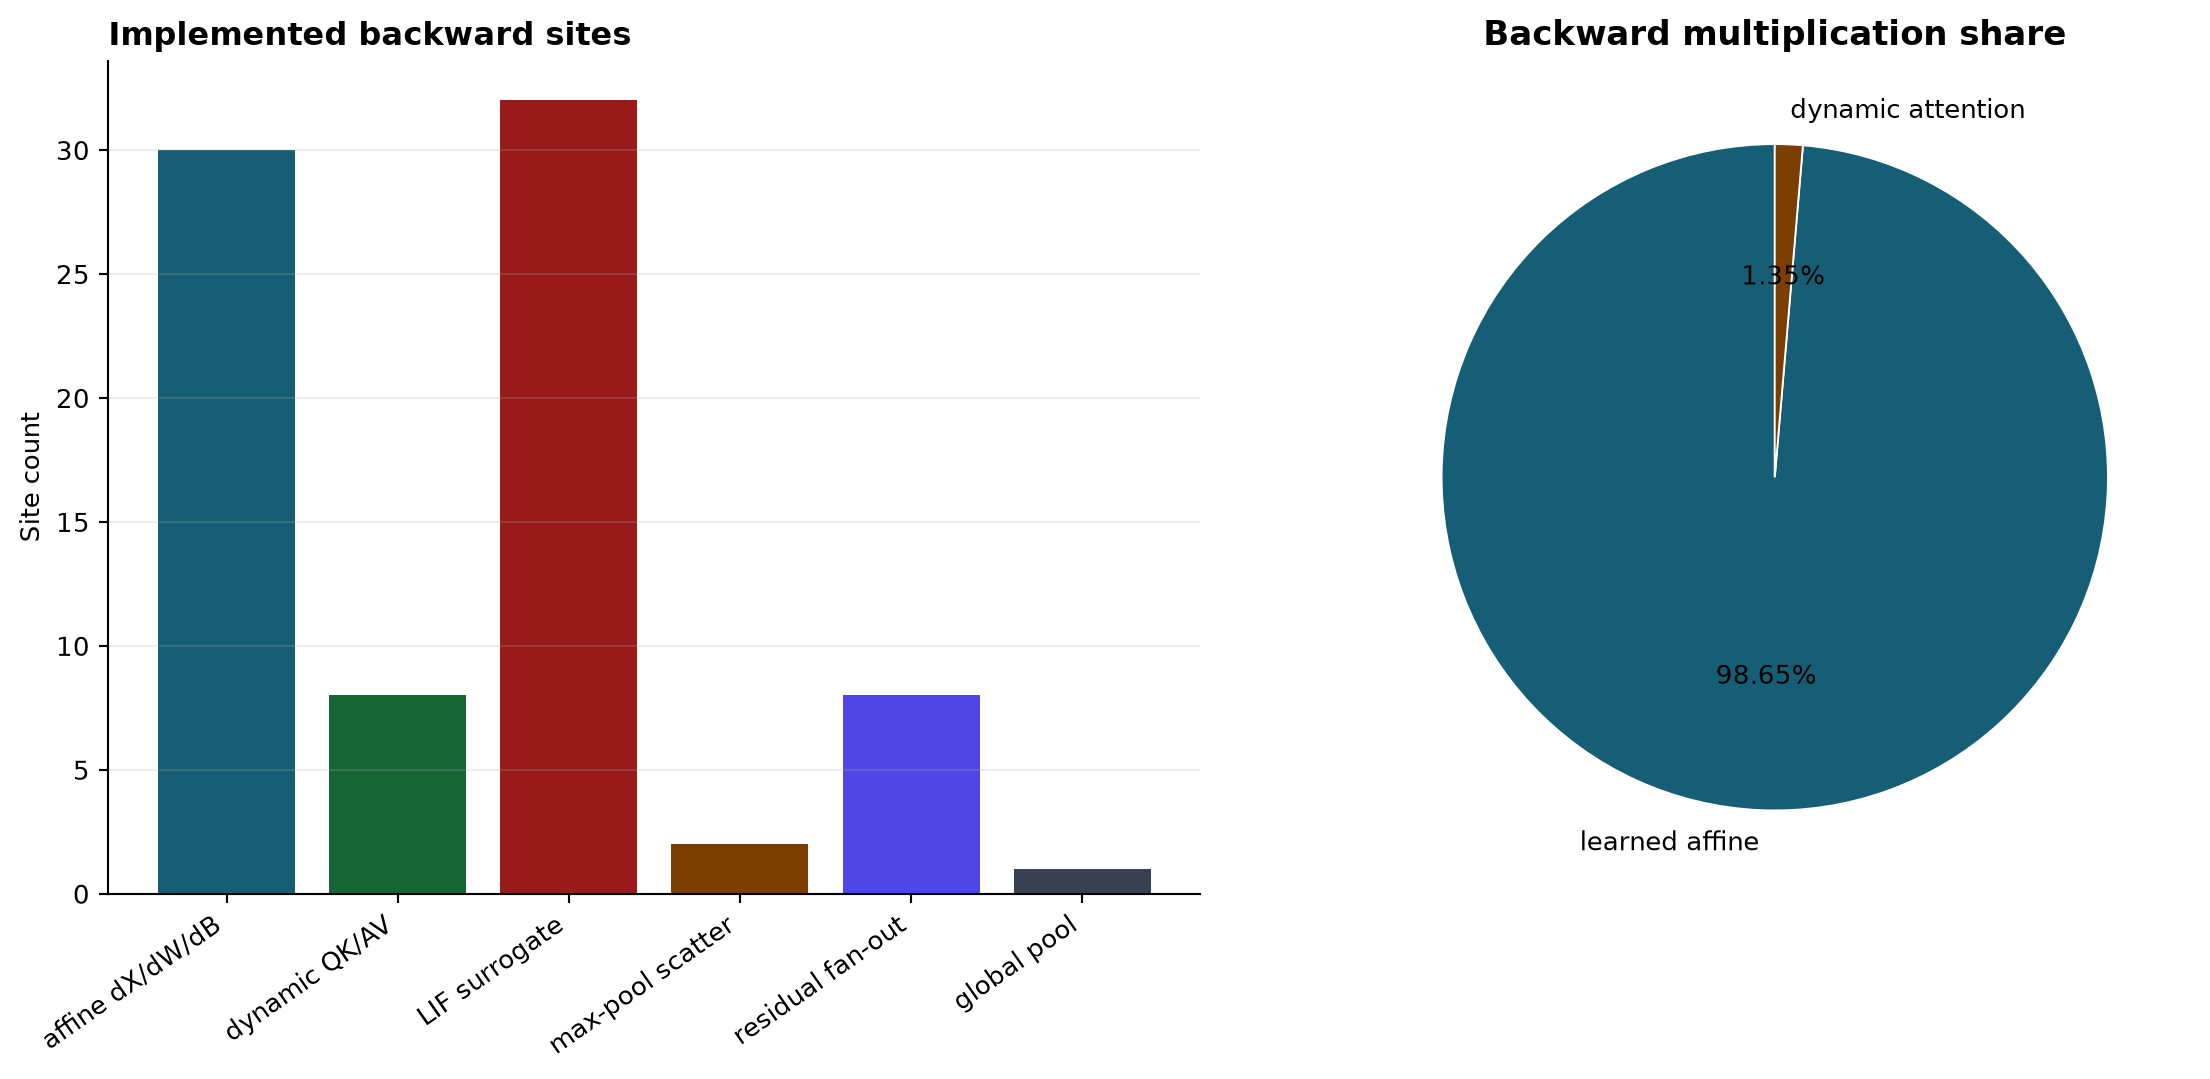
\includegraphics[width=0.98\textwidth,height=0.78\textheight,keepaspectratio]{plots/25_training_operator_coverage.png}
\end{center}
\clearpage
\section{Deterministic CIFAR-10 board-training shards}
\begin{sloppypar}\small\textbf{Evidence:} C:\textbackslash{}\allowbreak{}Users\textbackslash{}\allowbreak{}Ross\textbackslash{}\allowbreak{}Downloads\textbackslash{}\allowbreak{}neuraedge--main\textbackslash{}\allowbreak{}neuraedge--main\textbackslash{}\allowbreak{}neuraedge\_\allowbreak{}universal\textbackslash{}\allowbreak{}outputs\textbackslash{}\allowbreak{}cifar10\_\allowbreak{}shards\textbackslash{}\allowbreak{}cifar10\_\allowbreak{}shards\_\allowbreak{}manifest.json\end{sloppypar}
\begin{center}
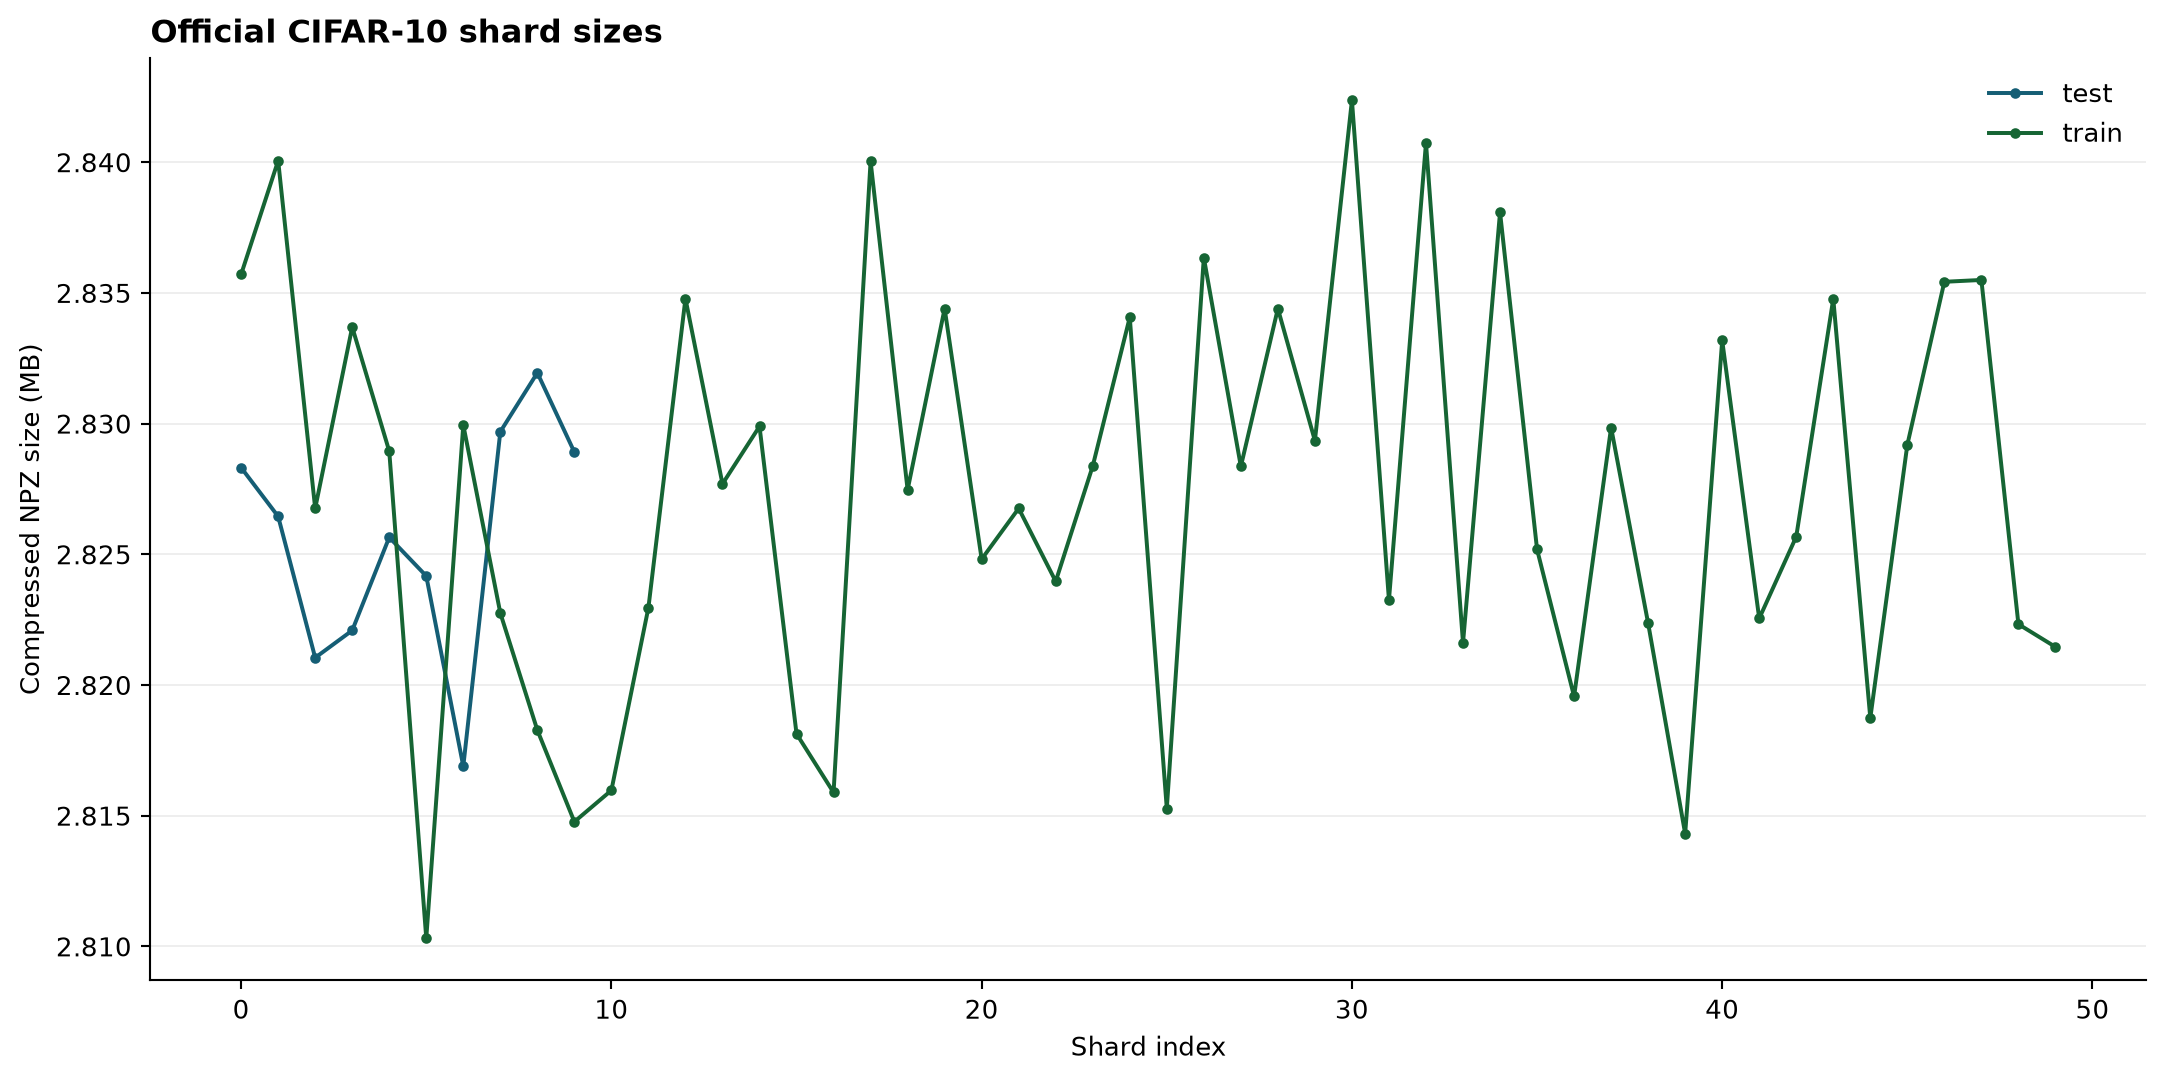
\includegraphics[width=0.98\textwidth,height=0.78\textheight,keepaspectratio]{plots/26_training_dataset_shards.png}
\end{center}
\clearpage
\section{Waveform: tb\_neuraedge\_mac2\_u8}
\begin{sloppypar}\small\textbf{Evidence:} Vivado 2026.1 XSim VCD,\allowbreak{} requested window 2 us;\allowbreak{} signals: dsp\_\allowbreak{}product\_\allowbreak{}valid\_\allowbreak{}r,\allowbreak{} packed\_\allowbreak{}product,\allowbreak{} product\_\allowbreak{}hi,\allowbreak{} product\_\allowbreak{}lo,\allowbreak{} product\_\allowbreak{}valid,\allowbreak{} product\_\allowbreak{}valid\_\allowbreak{}r,\allowbreak{} activation,\allowbreak{} extended\_\allowbreak{}activation\_\allowbreak{}r,\allowbreak{} packed\_\allowbreak{}weight\_\allowbreak{}r,\allowbreak{} weight\_\allowbreak{}hi\end{sloppypar}
\begin{center}
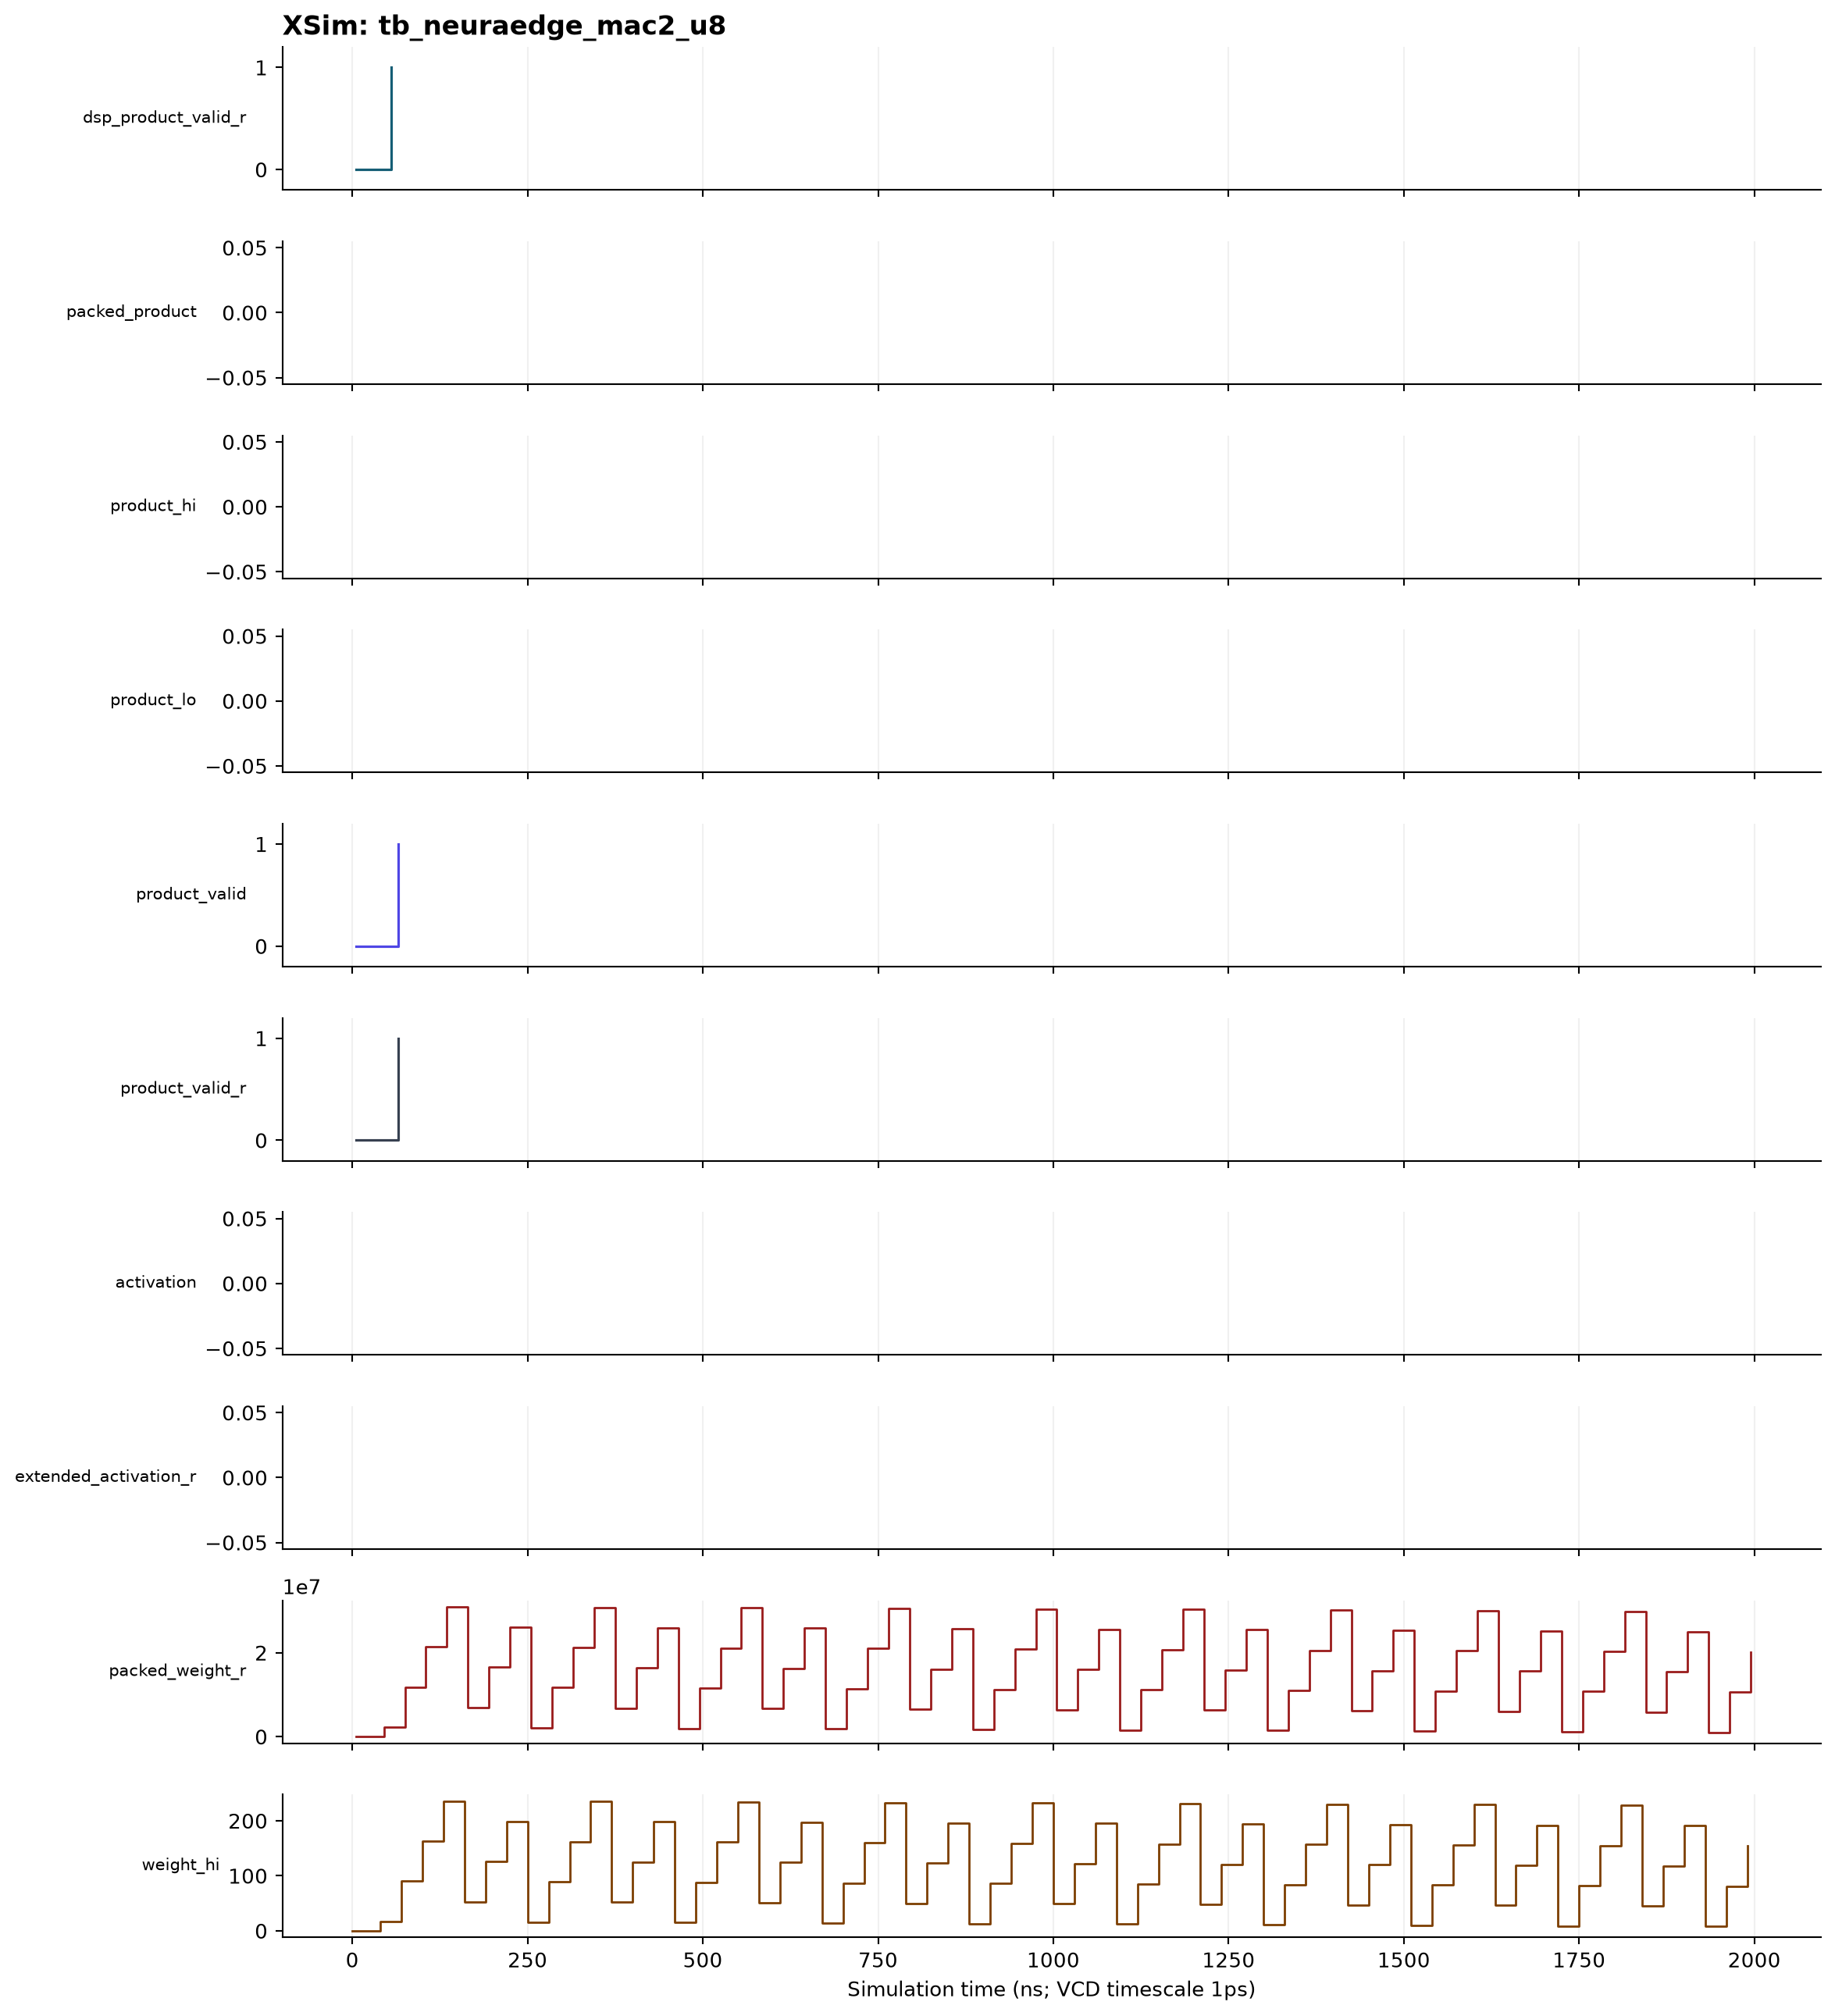
\includegraphics[width=0.98\textwidth,height=0.78\textheight,keepaspectratio]{plots/27_wave_mac2_u8.png}
\end{center}
\clearpage
\section{Waveform: tb\_neuraedge\_tensor\_tile}
\begin{sloppypar}\small\textbf{Evidence:} Vivado 2026.1 XSim VCD,\allowbreak{} requested window 3 us;\allowbreak{} signals: state,\allowbreak{} issue\_\allowbreak{}valid,\allowbreak{} issue\_\allowbreak{}ready,\allowbreak{} result\_\allowbreak{}valid,\allowbreak{} result\_\allowbreak{}ready,\allowbreak{} debug\_\allowbreak{}spike\_\allowbreak{}adds,\allowbreak{} debug\_\allowbreak{}spike\_\allowbreak{}adds\_\allowbreak{}r,\allowbreak{} spike\_\allowbreak{}value,\allowbreak{} debug\_\allowbreak{}dense\_\allowbreak{}macs,\allowbreak{} debug\_\allowbreak{}dense\_\allowbreak{}macs\_\allowbreak{}r\end{sloppypar}
\begin{center}
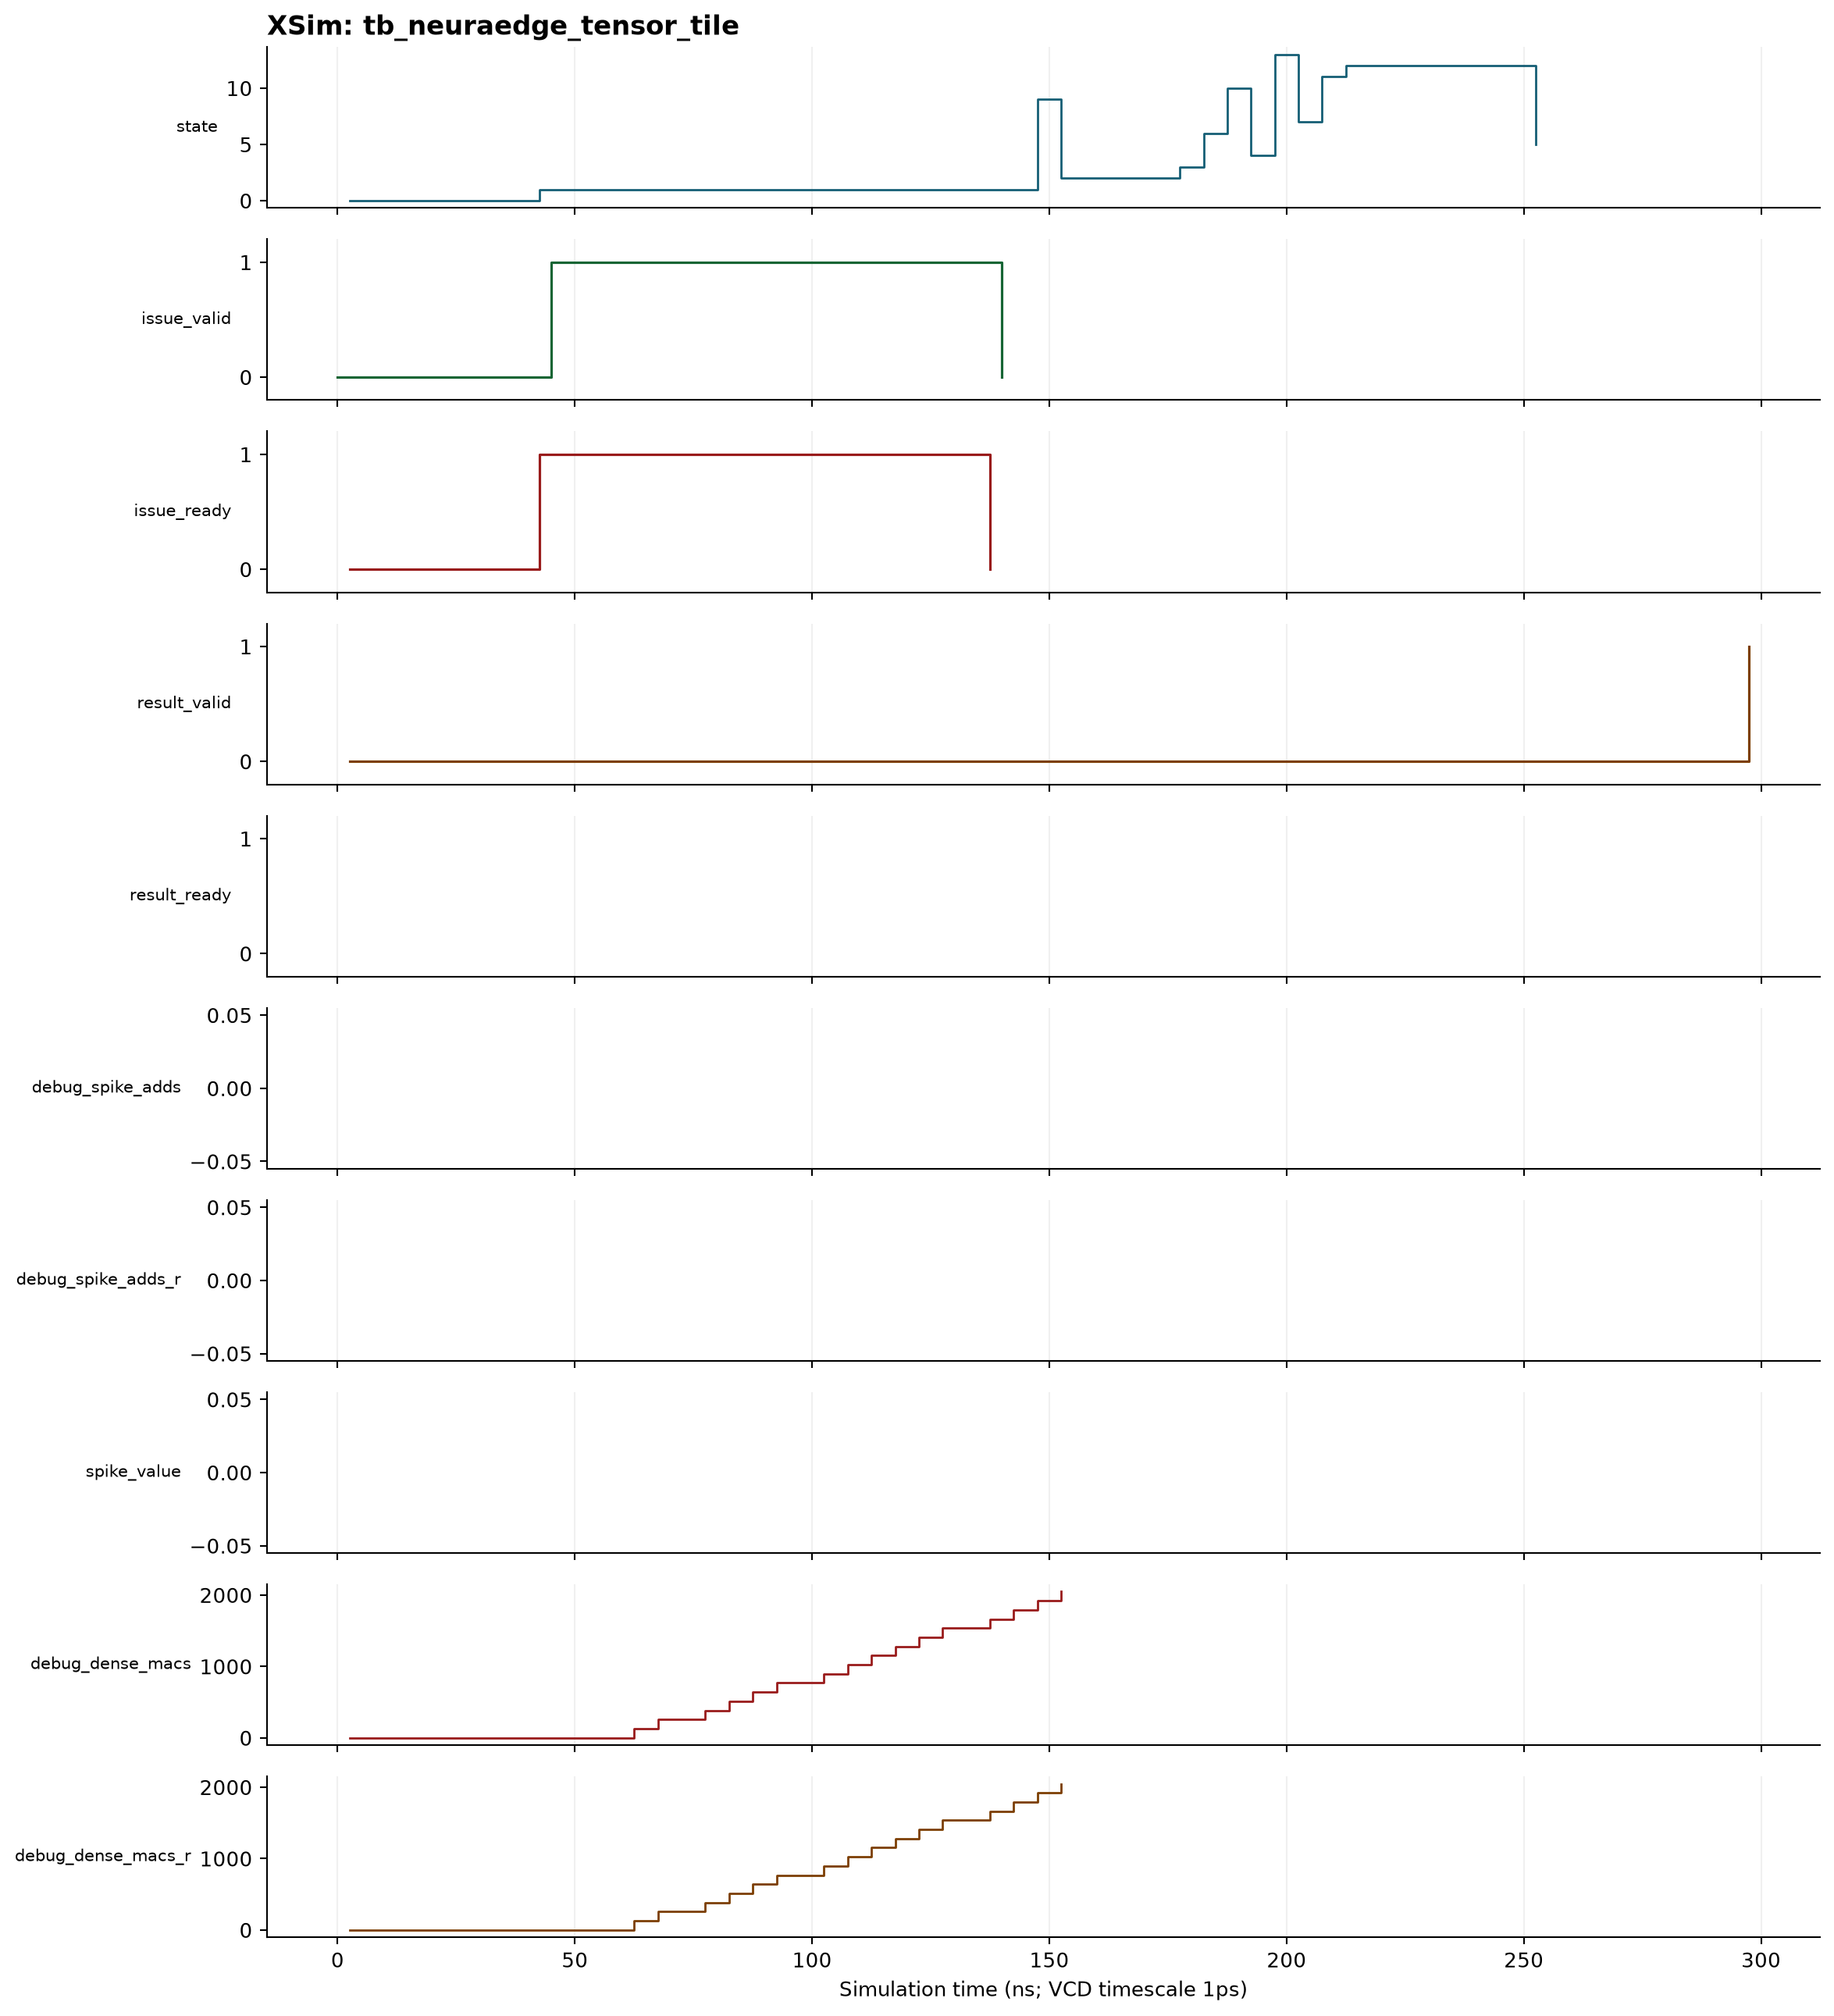
\includegraphics[width=0.98\textwidth,height=0.78\textheight,keepaspectratio]{plots/28_wave_tensor_tile.png}
\end{center}
\clearpage
\section{Waveform: tb\_neuraedge\_buffered\_tensor\_core}
\begin{sloppypar}\small\textbf{Evidence:} Vivado 2026.1 XSim VCD,\allowbreak{} requested window 4 us;\allowbreak{} signals: state,\allowbreak{} command\_\allowbreak{}valid,\allowbreak{} s\_\allowbreak{}axis\_\allowbreak{}tvalid,\allowbreak{} s\_\allowbreak{}axis\_\allowbreak{}tready,\allowbreak{} tile\_\allowbreak{}issue\_\allowbreak{}valid,\allowbreak{} issue\_\allowbreak{}valid,\allowbreak{} tile\_\allowbreak{}issue\_\allowbreak{}ready,\allowbreak{} issue\_\allowbreak{}ready,\allowbreak{} tile\_\allowbreak{}result\_\allowbreak{}valid,\allowbreak{} result\_\allowbreak{}valid\end{sloppypar}
\begin{center}
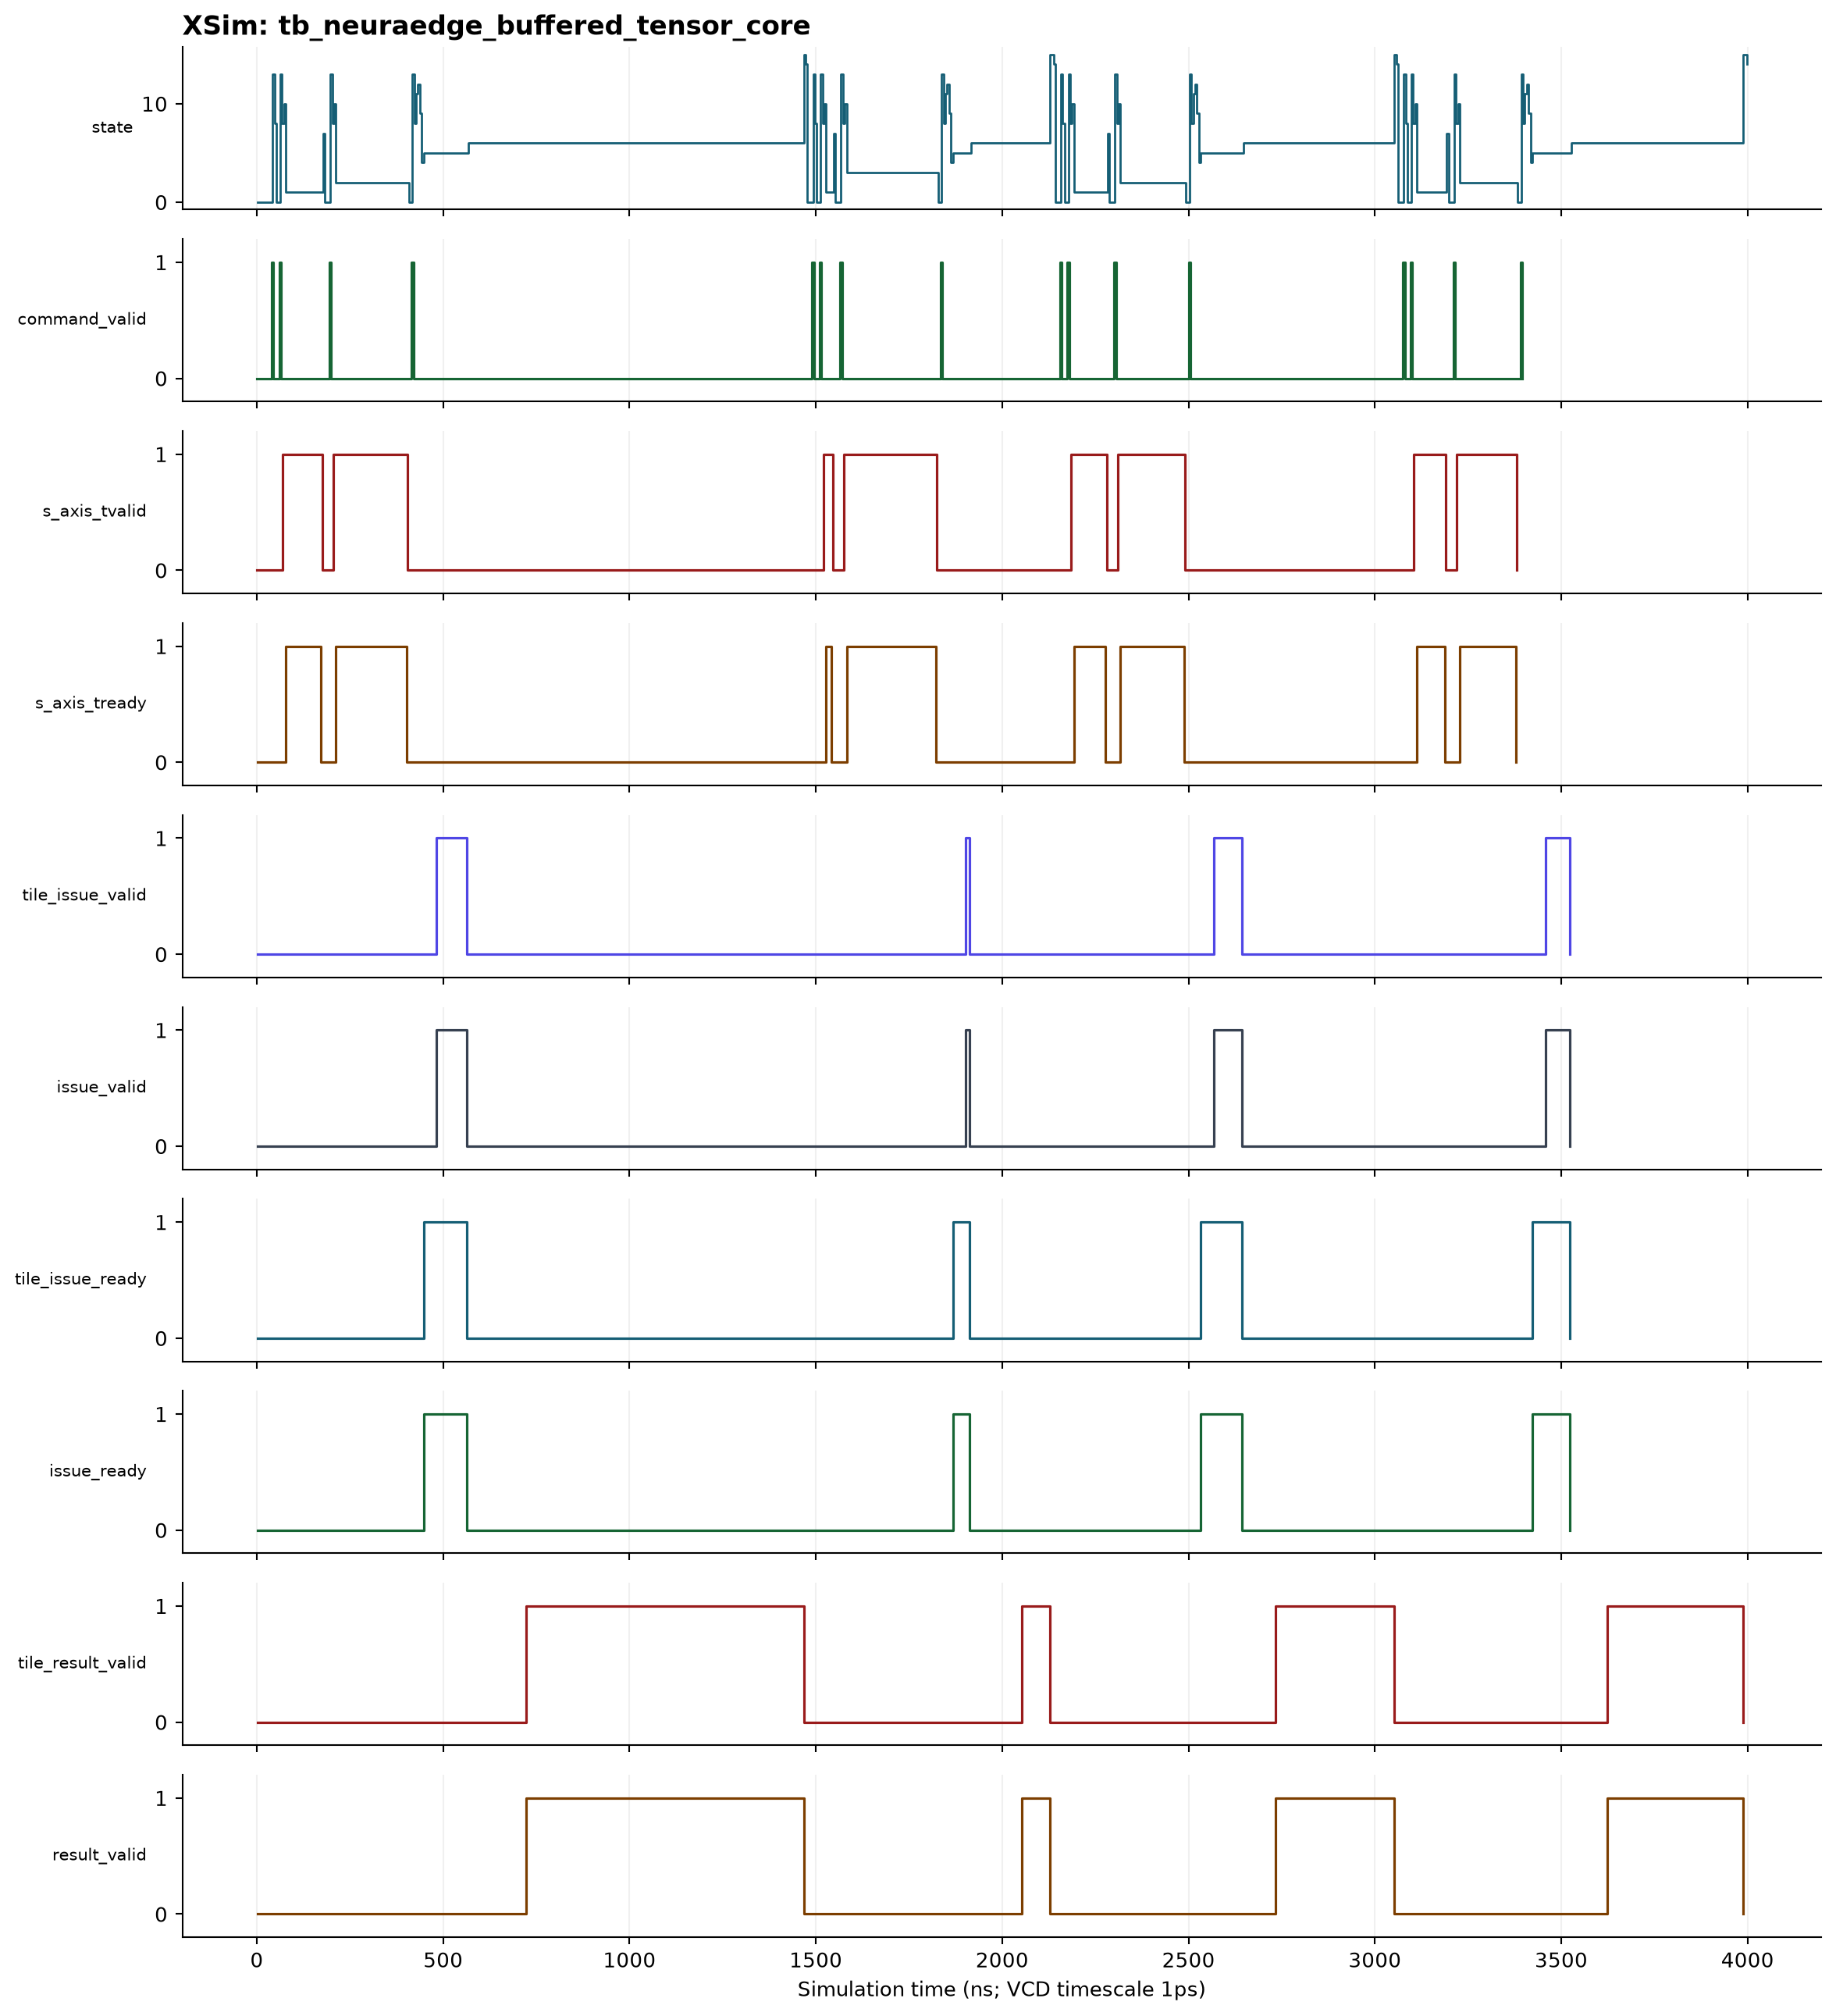
\includegraphics[width=0.98\textwidth,height=0.78\textheight,keepaspectratio]{plots/29_wave_buffered_tensor_core.png}
\end{center}
\clearpage
\section{Waveform: tb\_neuraedge\_alpha\_xnor}
\begin{sloppypar}\small\textbf{Evidence:} Vivado 2026.1 XSim VCD,\allowbreak{} requested window 40 us;\allowbreak{} signals: state,\allowbreak{} output\_\allowbreak{}valid,\allowbreak{} output\_\allowbreak{}ready,\allowbreak{} final\_\allowbreak{}spike\_\allowbreak{}count\_\allowbreak{}r,\allowbreak{} key\_\allowbreak{}spikes,\allowbreak{} query\_\allowbreak{}spikes,\allowbreak{} score\_\allowbreak{}spike\_\allowbreak{}operand\_\allowbreak{}r,\allowbreak{} spike\_\allowbreak{}chunk\_\allowbreak{}count\_\allowbreak{}r,\allowbreak{} spike\_\allowbreak{}count\_\allowbreak{}r,\allowbreak{} spike\_\allowbreak{}mask\_\allowbreak{}r\end{sloppypar}
\begin{center}
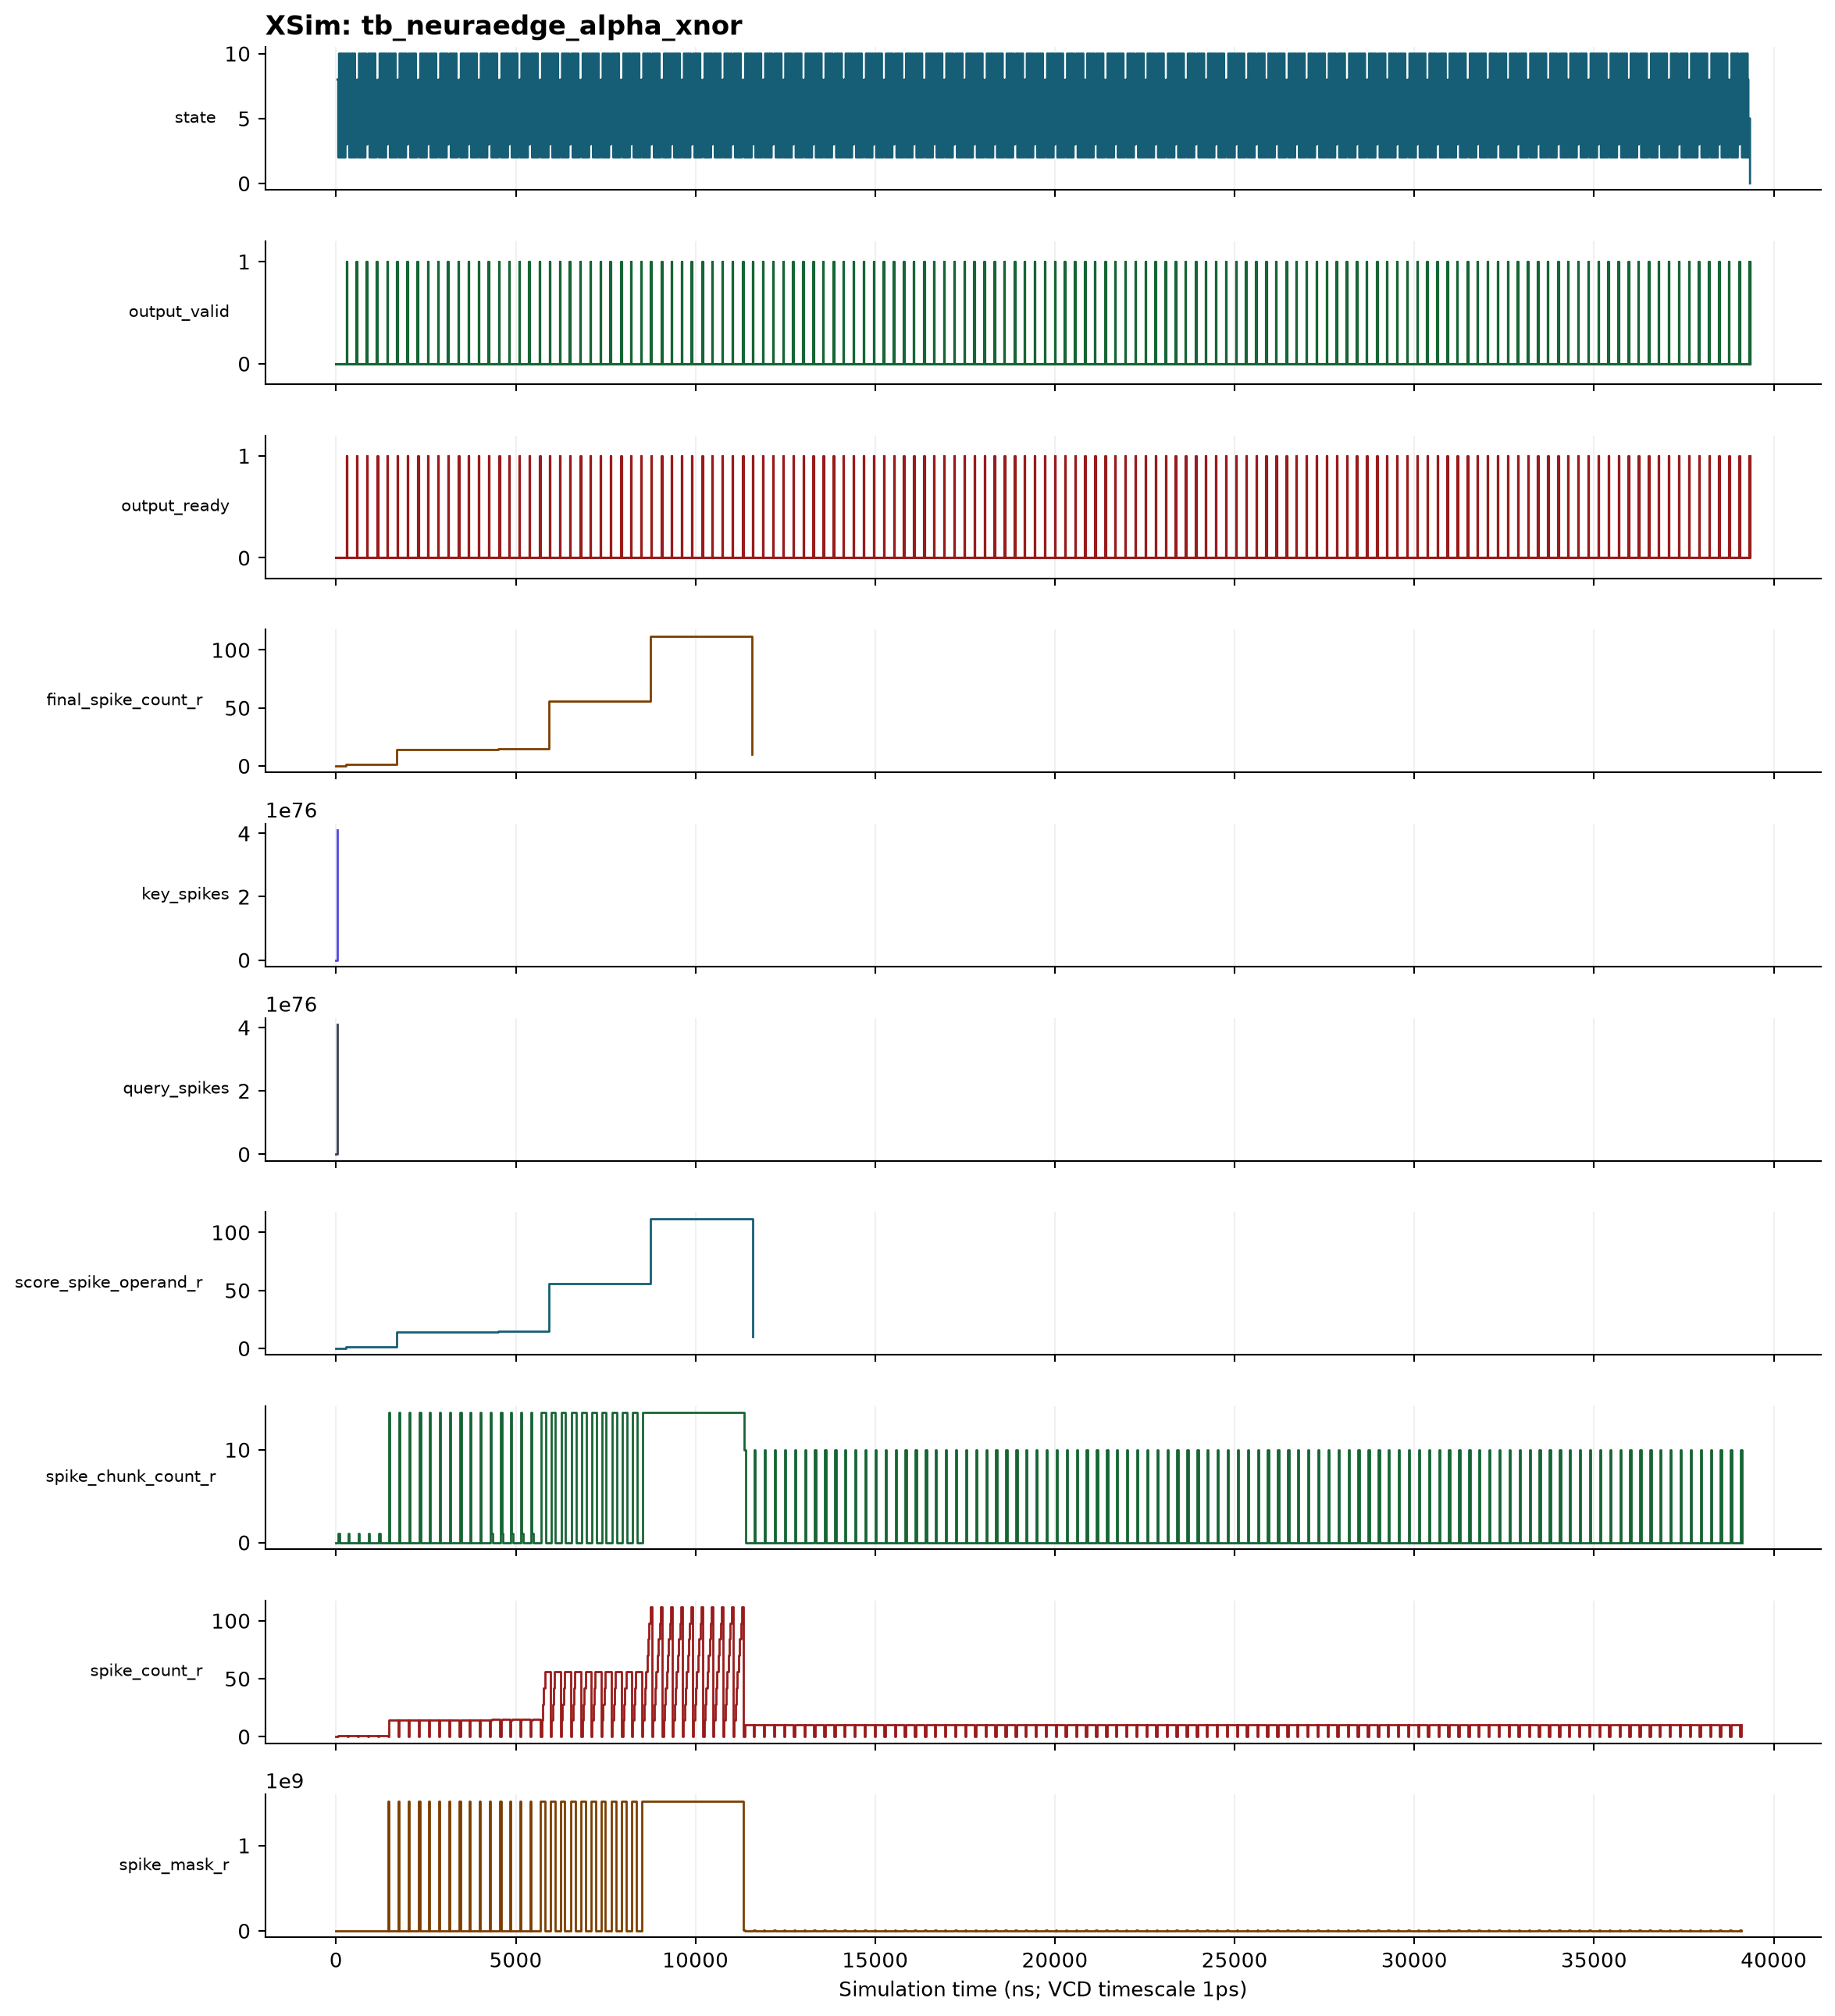
\includegraphics[width=0.98\textwidth,height=0.78\textheight,keepaspectratio]{plots/30_wave_alpha_xnor.png}
\end{center}
\clearpage
\section{Waveform: tb\_neuraedge\_vector\_alu}
\begin{sloppypar}\small\textbf{Evidence:} Vivado 2026.1 XSim VCD,\allowbreak{} requested window 170 us;\allowbreak{} signals: state,\allowbreak{} output\_\allowbreak{}valid,\allowbreak{} output\_\allowbreak{}ready,\allowbreak{} OP\_\allowbreak{}BINARY\_\allowbreak{}SPIKE,\allowbreak{} OP\_\allowbreak{}TERNARY\_\allowbreak{}SPIKE,\allowbreak{} multiplier\_\allowbreak{}product\_\allowbreak{}hh,\allowbreak{} multiplier\_\allowbreak{}product\_\allowbreak{}hl,\allowbreak{} multiplier\_\allowbreak{}product\_\allowbreak{}lh,\allowbreak{} multiplier\_\allowbreak{}product\_\allowbreak{}ll,\allowbreak{} product\_\allowbreak{}cross\_\allowbreak{}r\end{sloppypar}
\begin{center}
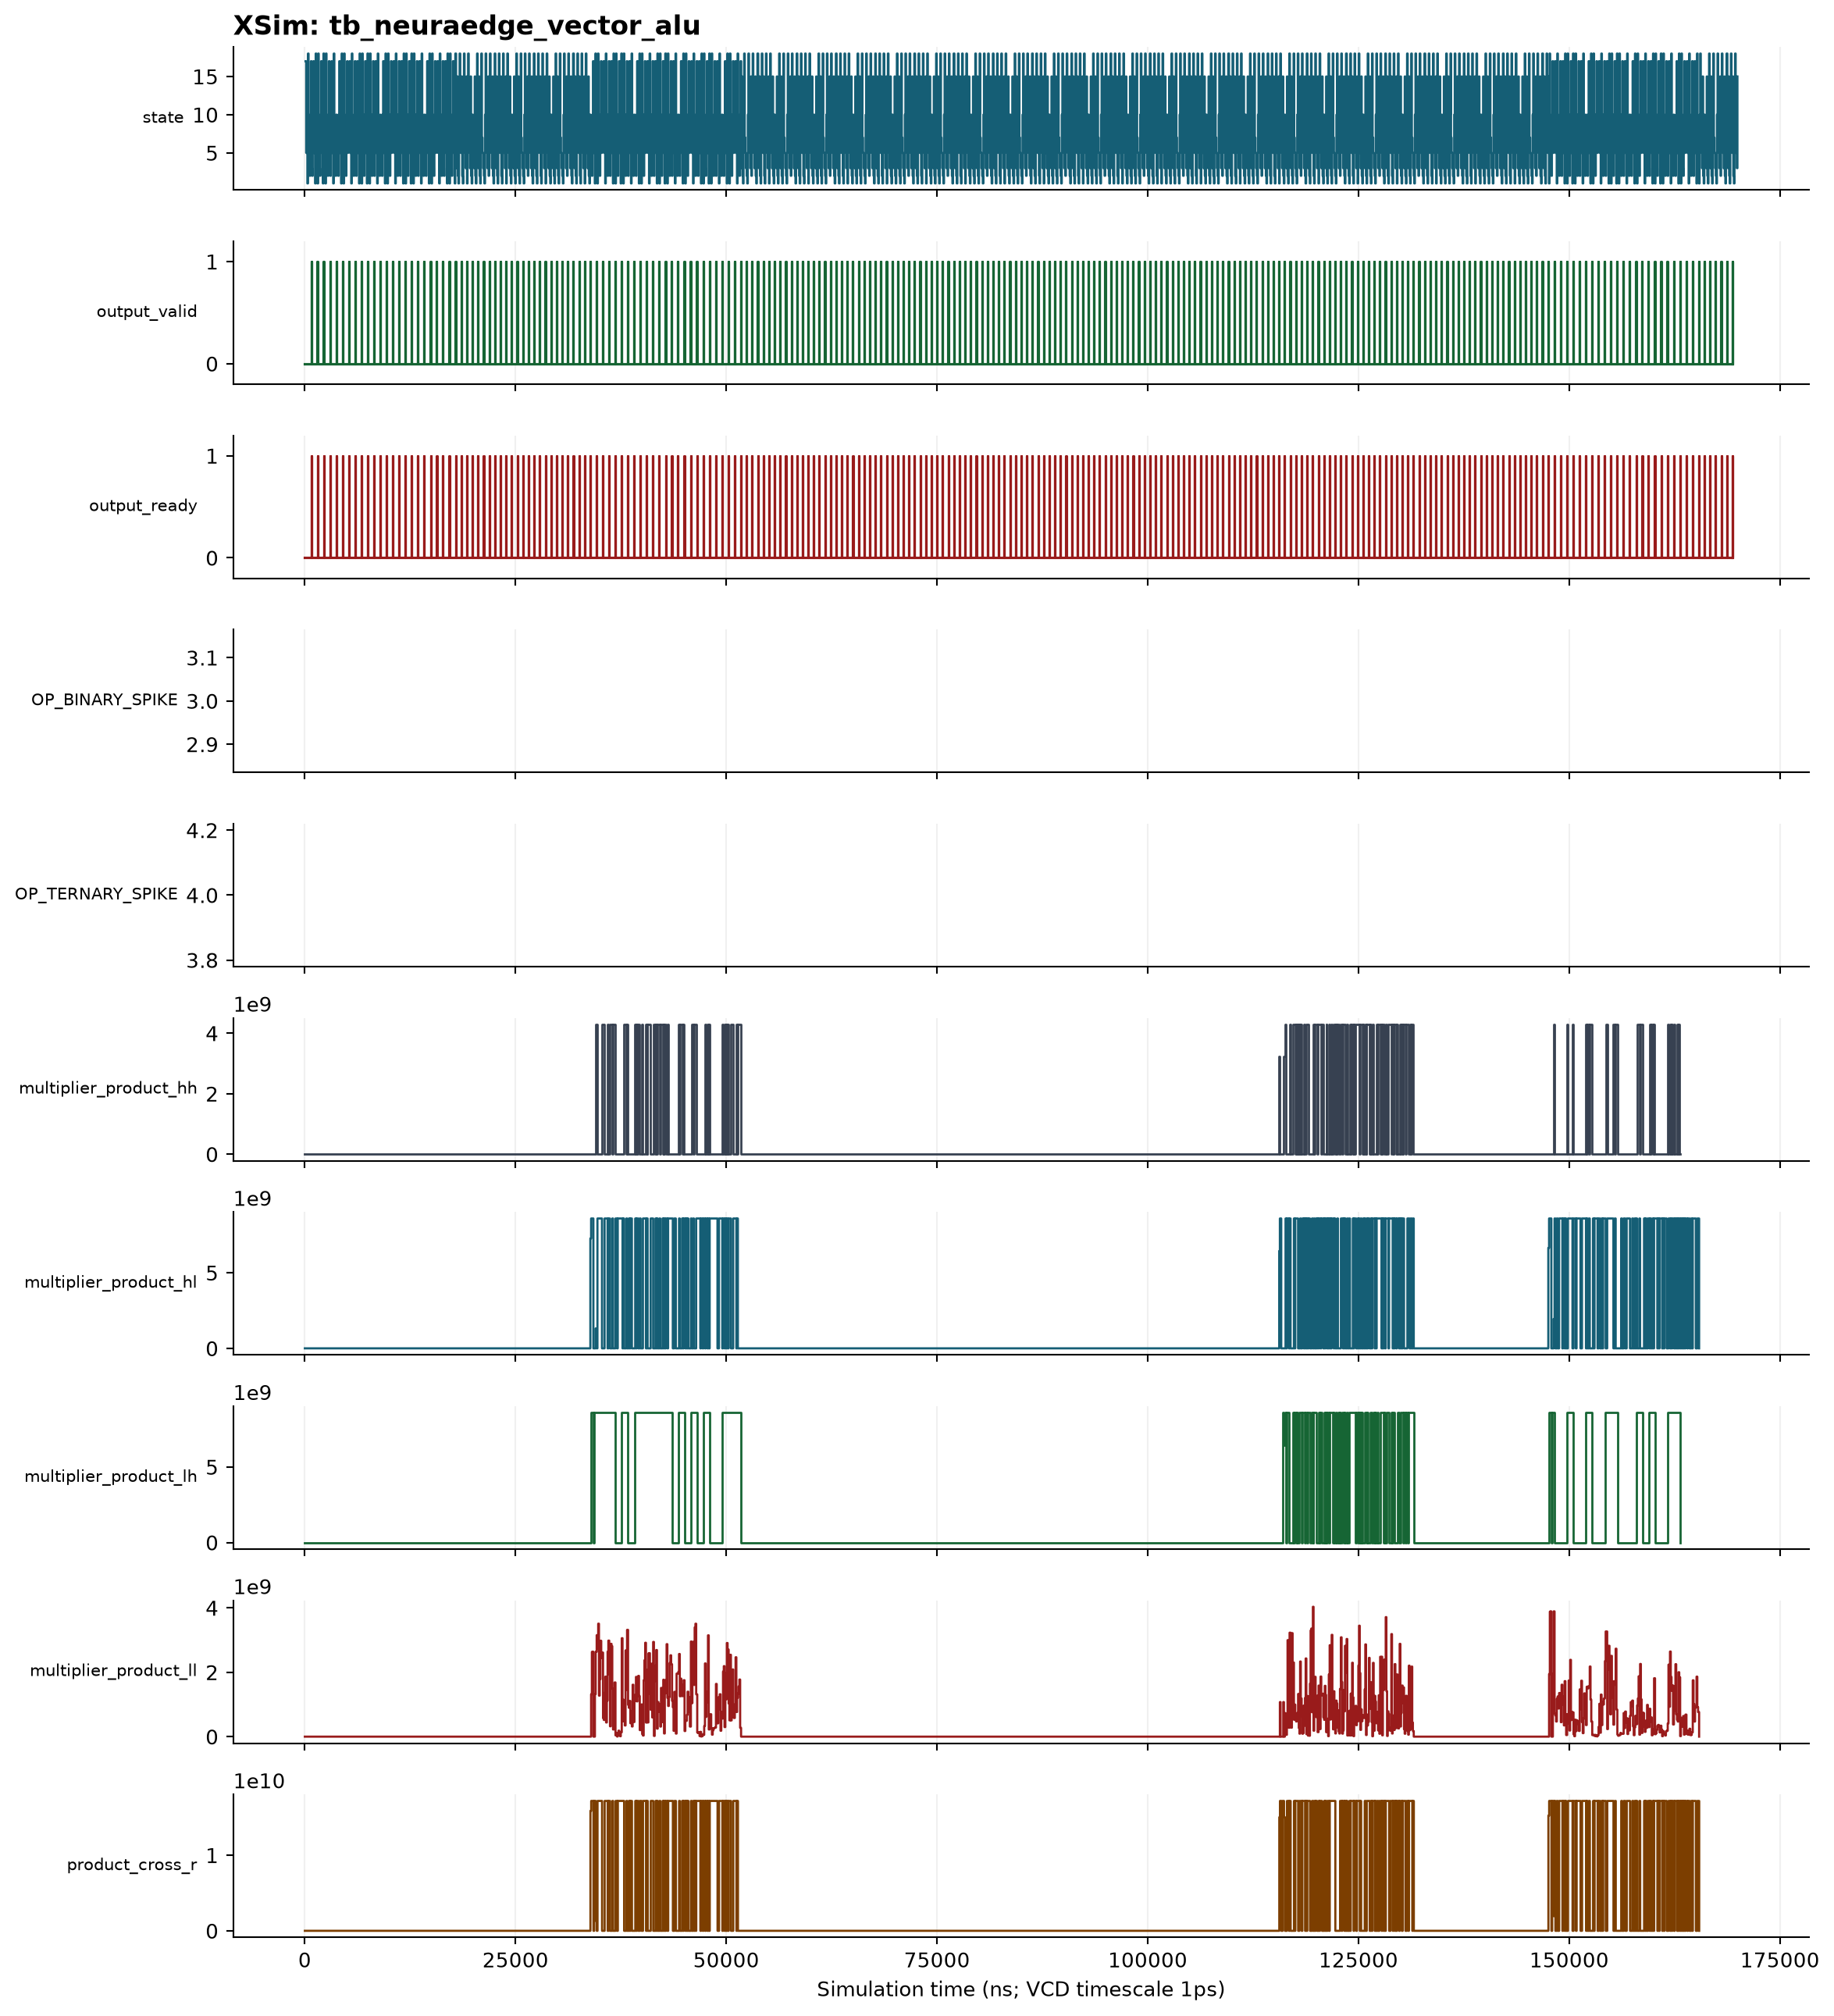
\includegraphics[width=0.98\textwidth,height=0.78\textheight,keepaspectratio]{plots/31_wave_vector_alu.png}
\end{center}
\clearpage
\section{Waveform: tb\_neuraedge\_integer\_primitives}
\begin{sloppypar}\small\textbf{Evidence:} Vivado 2026.1 XSim VCD,\allowbreak{} requested window 90 us;\allowbreak{} signals: state,\allowbreak{} div\_\allowbreak{}output\_\allowbreak{}valid,\allowbreak{} sqrt\_\allowbreak{}output\_\allowbreak{}valid,\allowbreak{} output\_\allowbreak{}valid,\allowbreak{} div\_\allowbreak{}output\_\allowbreak{}ready,\allowbreak{} sqrt\_\allowbreak{}output\_\allowbreak{}ready,\allowbreak{} output\_\allowbreak{}ready\end{sloppypar}
\begin{center}
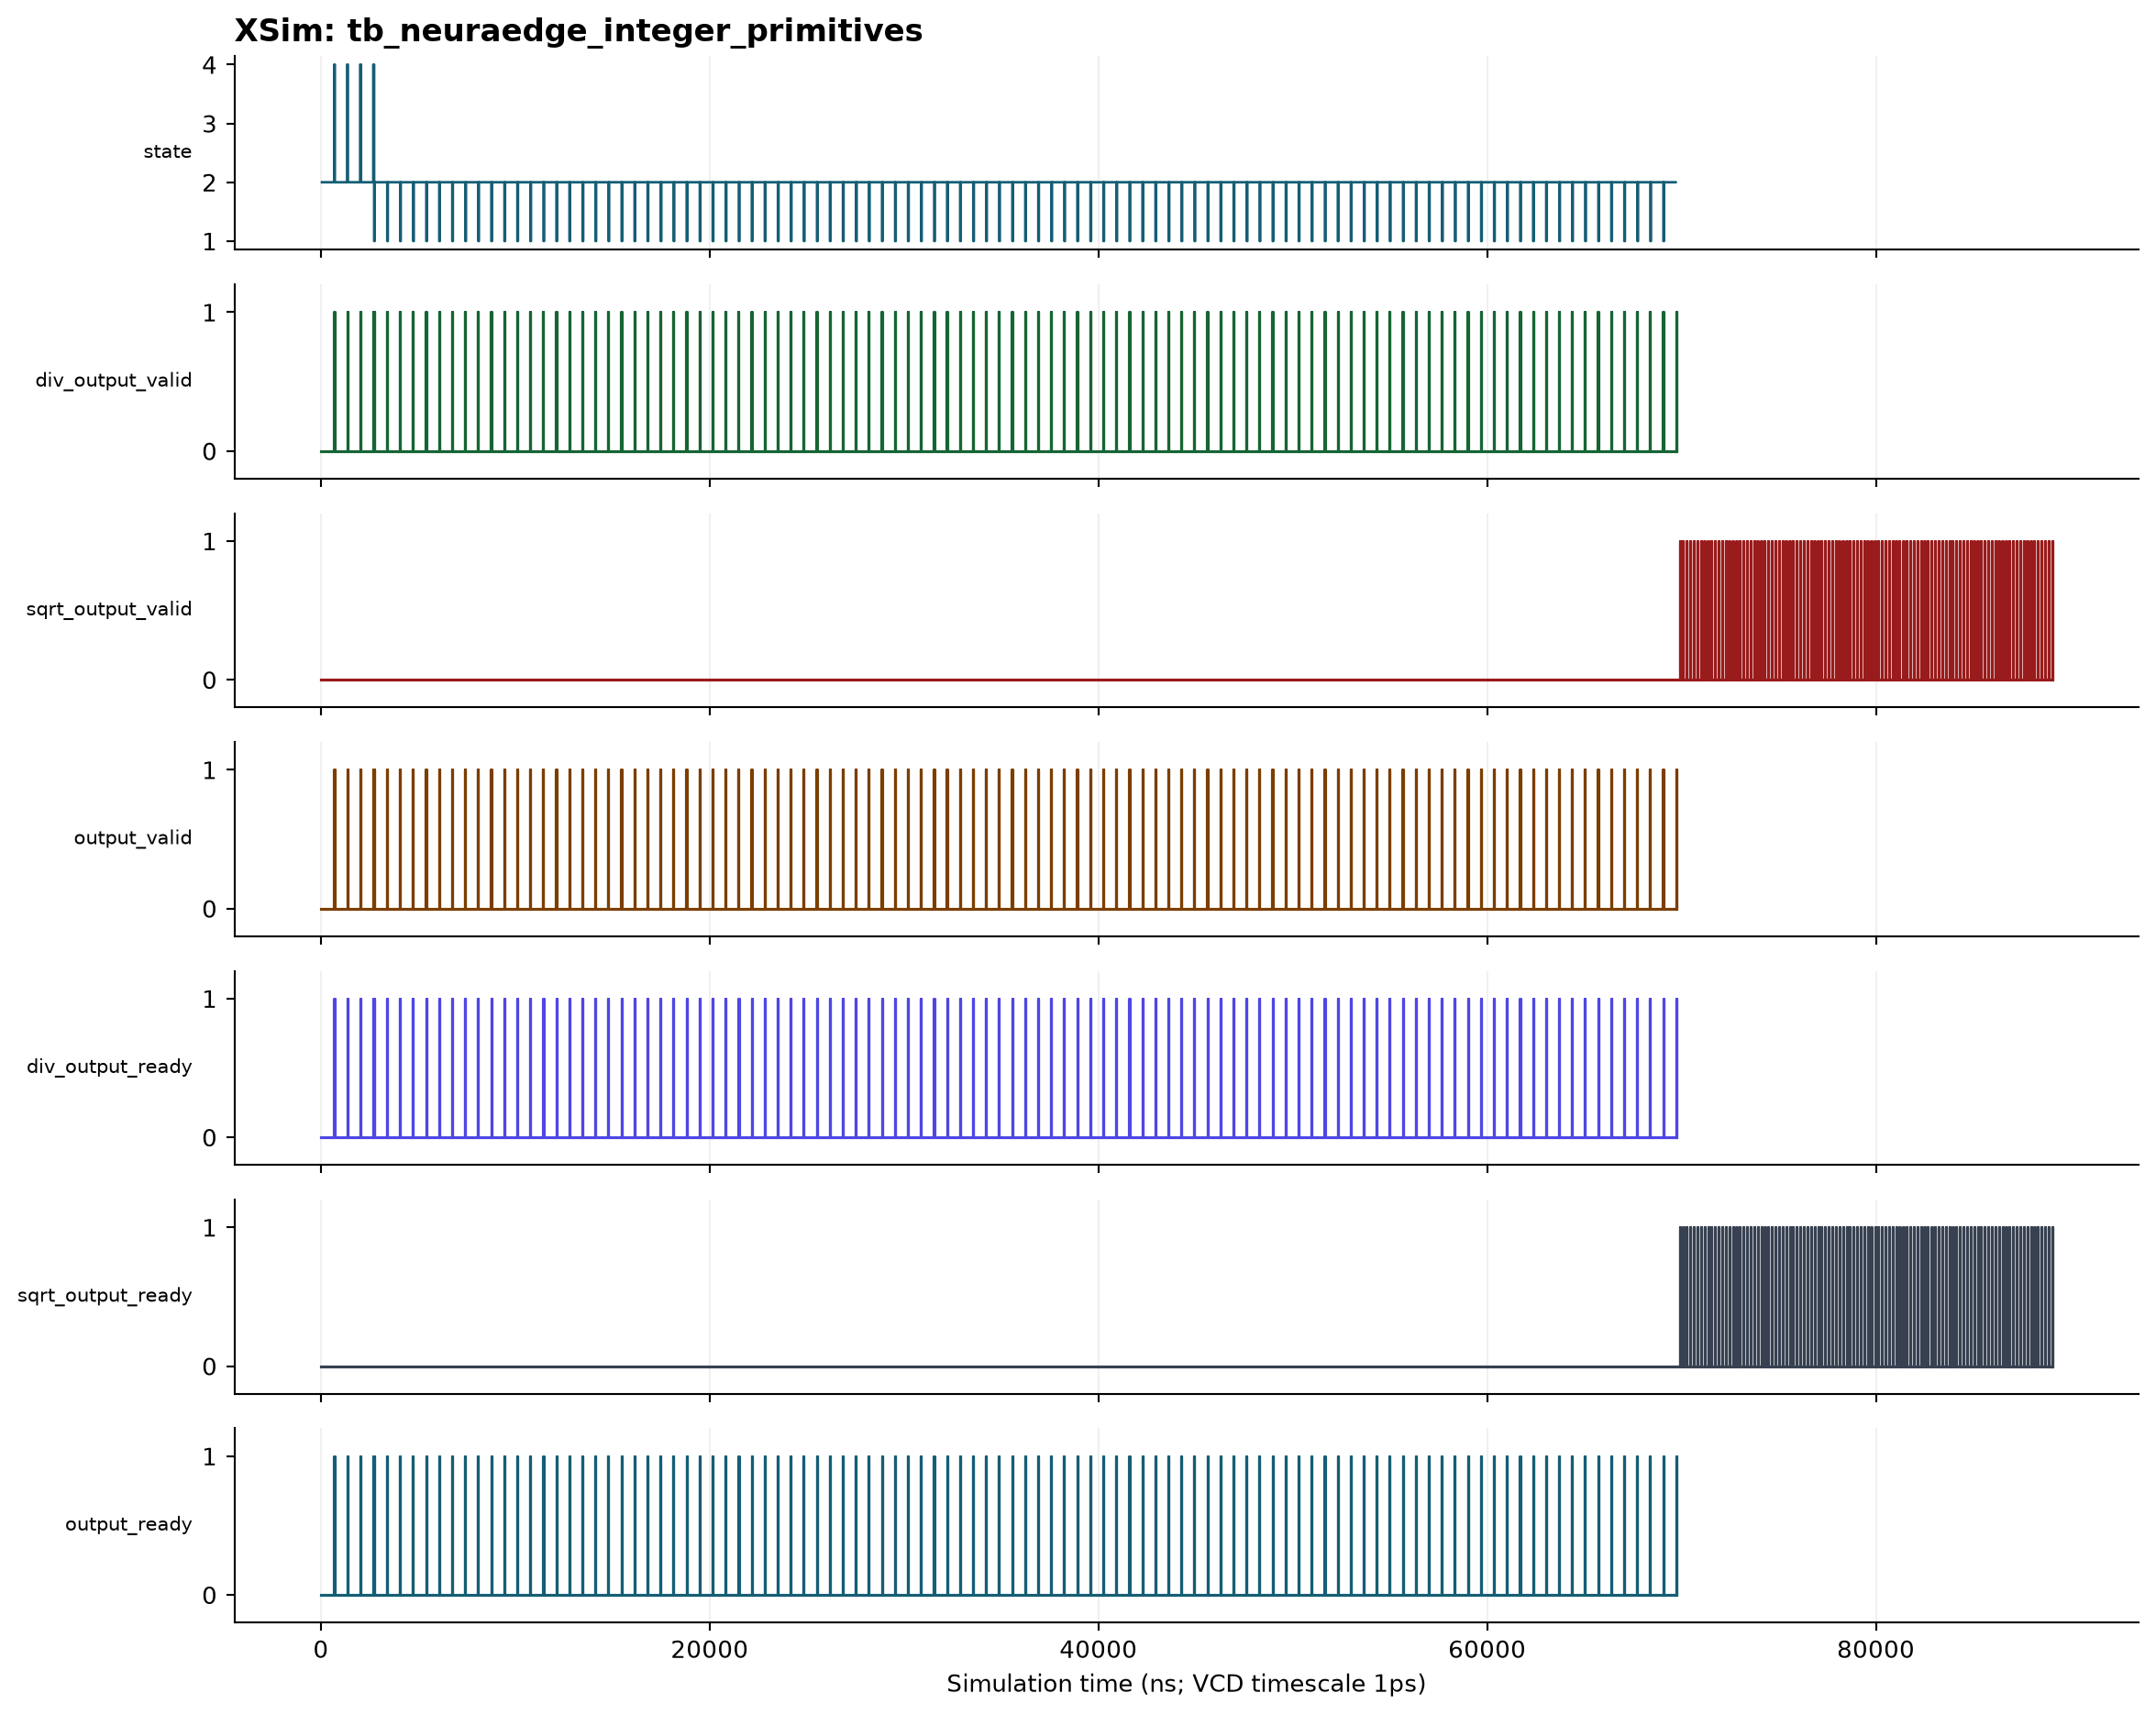
\includegraphics[width=0.98\textwidth,height=0.78\textheight,keepaspectratio]{plots/32_wave_integer_primitives.png}
\end{center}
\clearpage
\section{Waveform: tb\_neuraedge\_normalization\_units}
\begin{sloppypar}\small\textbf{Evidence:} Vivado 2026.1 XSim VCD,\allowbreak{} requested window 405 us;\allowbreak{} signals: state,\allowbreak{} ln\_\allowbreak{}result\_\allowbreak{}valid,\allowbreak{} result\_\allowbreak{}valid,\allowbreak{} ln\_\allowbreak{}result\_\allowbreak{}ready,\allowbreak{} result\_\allowbreak{}ready,\allowbreak{} divider\_\allowbreak{}output\_\allowbreak{}valid,\allowbreak{} sqrt\_\allowbreak{}output\_\allowbreak{}valid,\allowbreak{} output\_\allowbreak{}valid,\allowbreak{} divider\_\allowbreak{}output\_\allowbreak{}ready,\allowbreak{} sqrt\_\allowbreak{}output\_\allowbreak{}ready\end{sloppypar}
\begin{center}
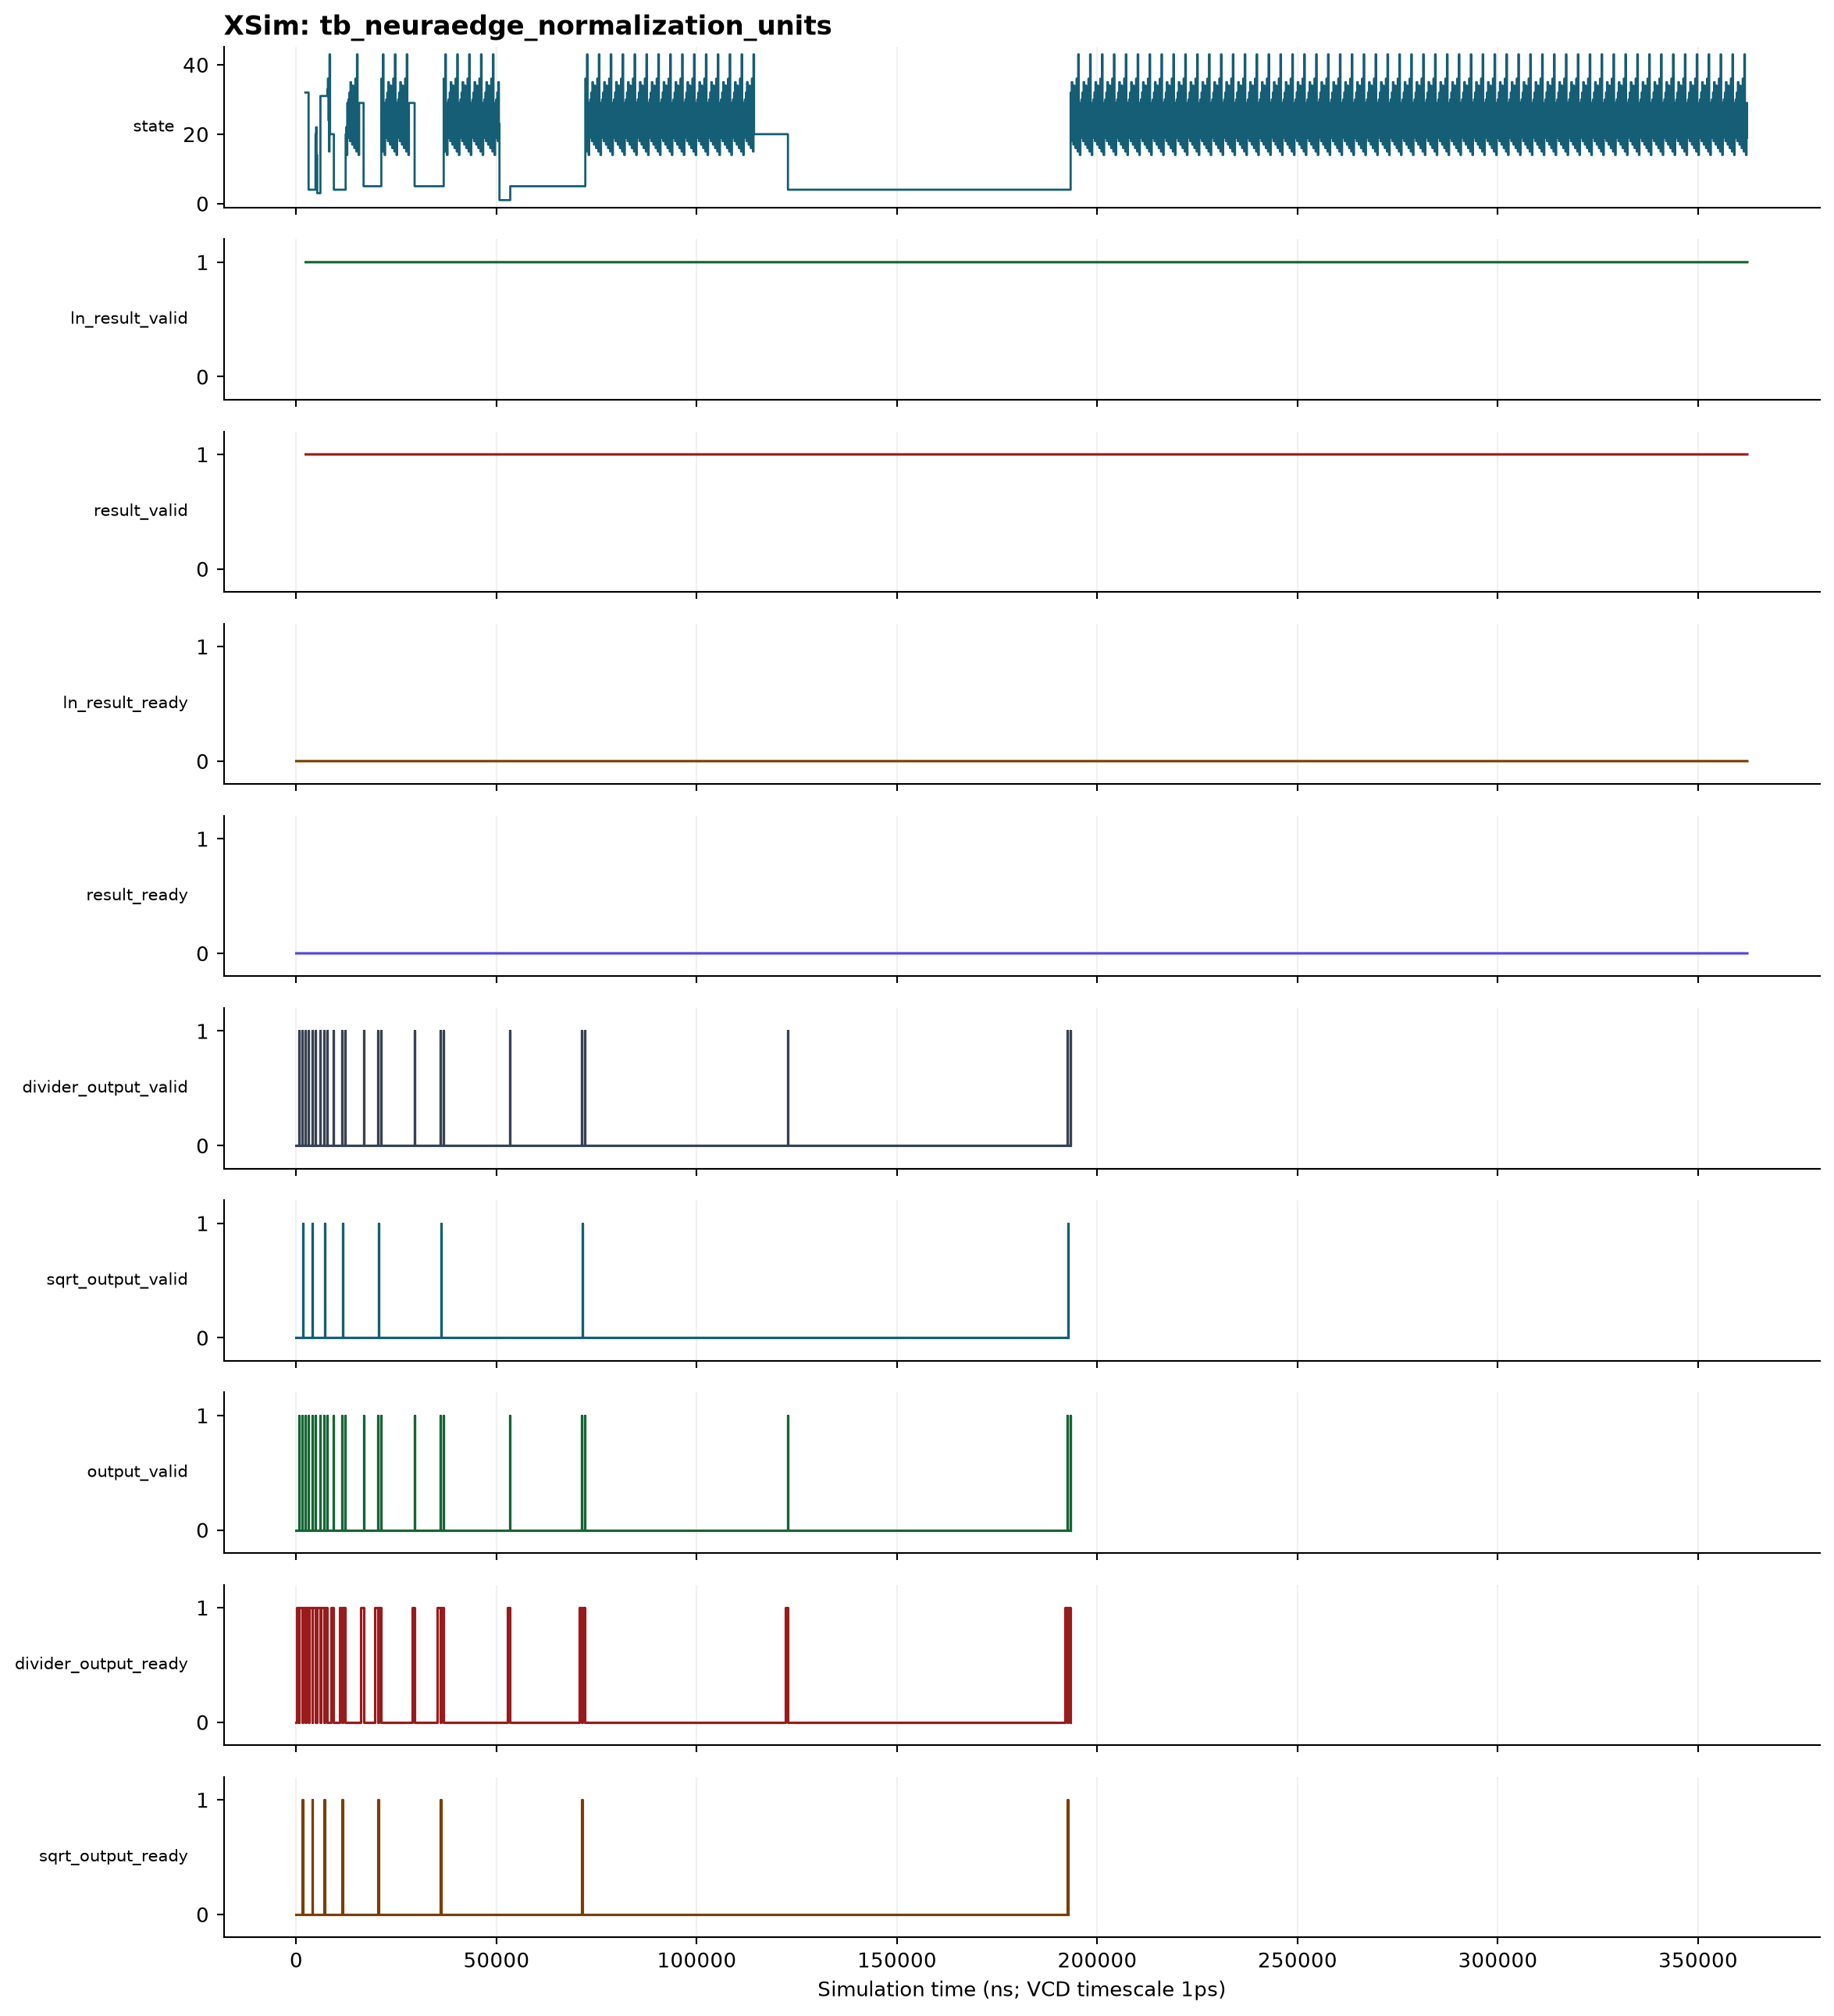
\includegraphics[width=0.98\textwidth,height=0.78\textheight,keepaspectratio]{plots/33_wave_normalization_units.png}
\end{center}
\clearpage
\section{Waveform: tb\_neuraedge\_lif\_bank}
\begin{sloppypar}\small\textbf{Evidence:} Vivado 2026.1 XSim VCD,\allowbreak{} requested window 20 us;\allowbreak{} signals: state,\allowbreak{} output\_\allowbreak{}valid,\allowbreak{} output\_\allowbreak{}ready,\allowbreak{} completed\_\allowbreak{}step\_\allowbreak{}spike\_\allowbreak{}count\_\allowbreak{}r,\allowbreak{} group\_\allowbreak{}spikes\_\allowbreak{}r,\allowbreak{} spike\_\allowbreak{}work\_\allowbreak{}r,\allowbreak{} spikes,\allowbreak{} step\_\allowbreak{}spike\_\allowbreak{}count\_\allowbreak{}r,\allowbreak{} total\_\allowbreak{}spike\_\allowbreak{}count,\allowbreak{} group\_\allowbreak{}spike\_\allowbreak{}count\end{sloppypar}
\begin{center}
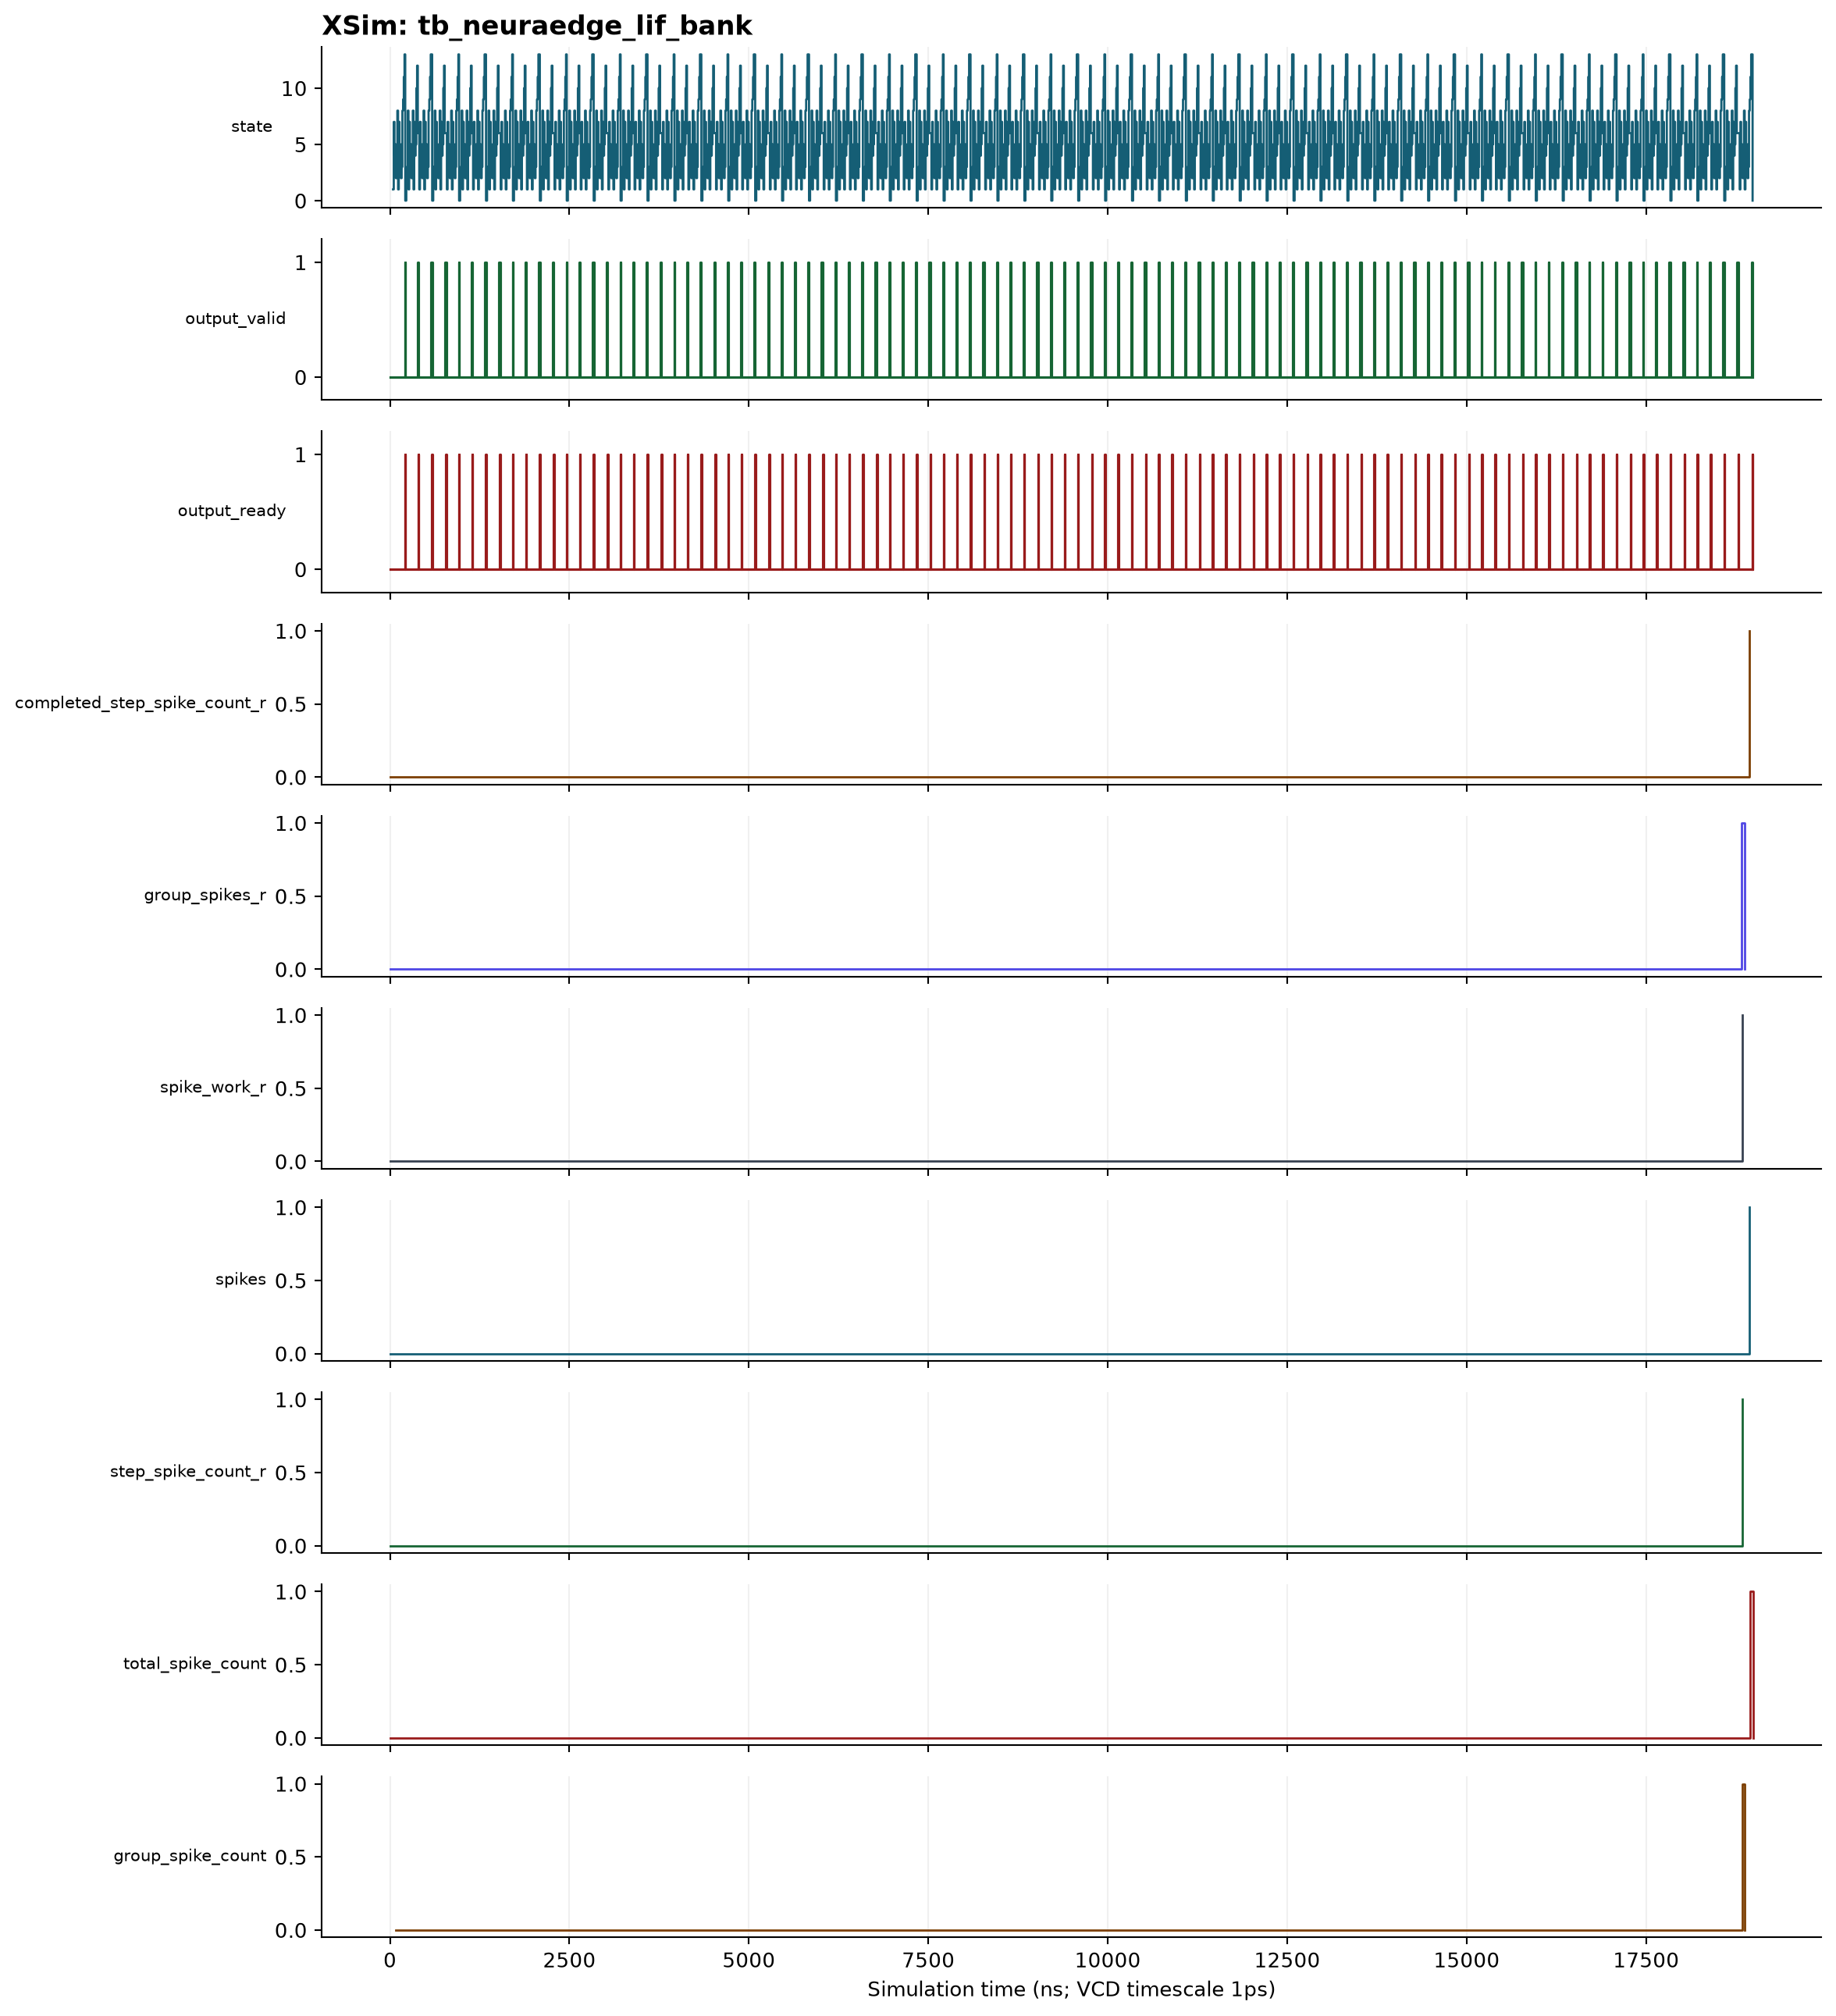
\includegraphics[width=0.98\textwidth,height=0.78\textheight,keepaspectratio]{plots/34_wave_lif_bank.png}
\end{center}
\clearpage
\section{Waveform: tb\_neuraedge\_linear\_backward8}
\begin{sloppypar}\small\textbf{Evidence:} Vivado 2026.1 XSim VCD,\allowbreak{} requested window 1 ms;\allowbreak{} signals: state,\allowbreak{} s\_\allowbreak{}axis\_\allowbreak{}tvalid,\allowbreak{} s\_\allowbreak{}axis\_\allowbreak{}tready,\allowbreak{} m\_\allowbreak{}axis\_\allowbreak{}tlast,\allowbreak{} MODE\_\allowbreak{}WEIGHT\_\allowbreak{}GRADIENT,\allowbreak{} packed\_\allowbreak{}weight\_\allowbreak{}gradient,\allowbreak{} weight\_\allowbreak{}gradient\_\allowbreak{}shift\end{sloppypar}
\begin{center}
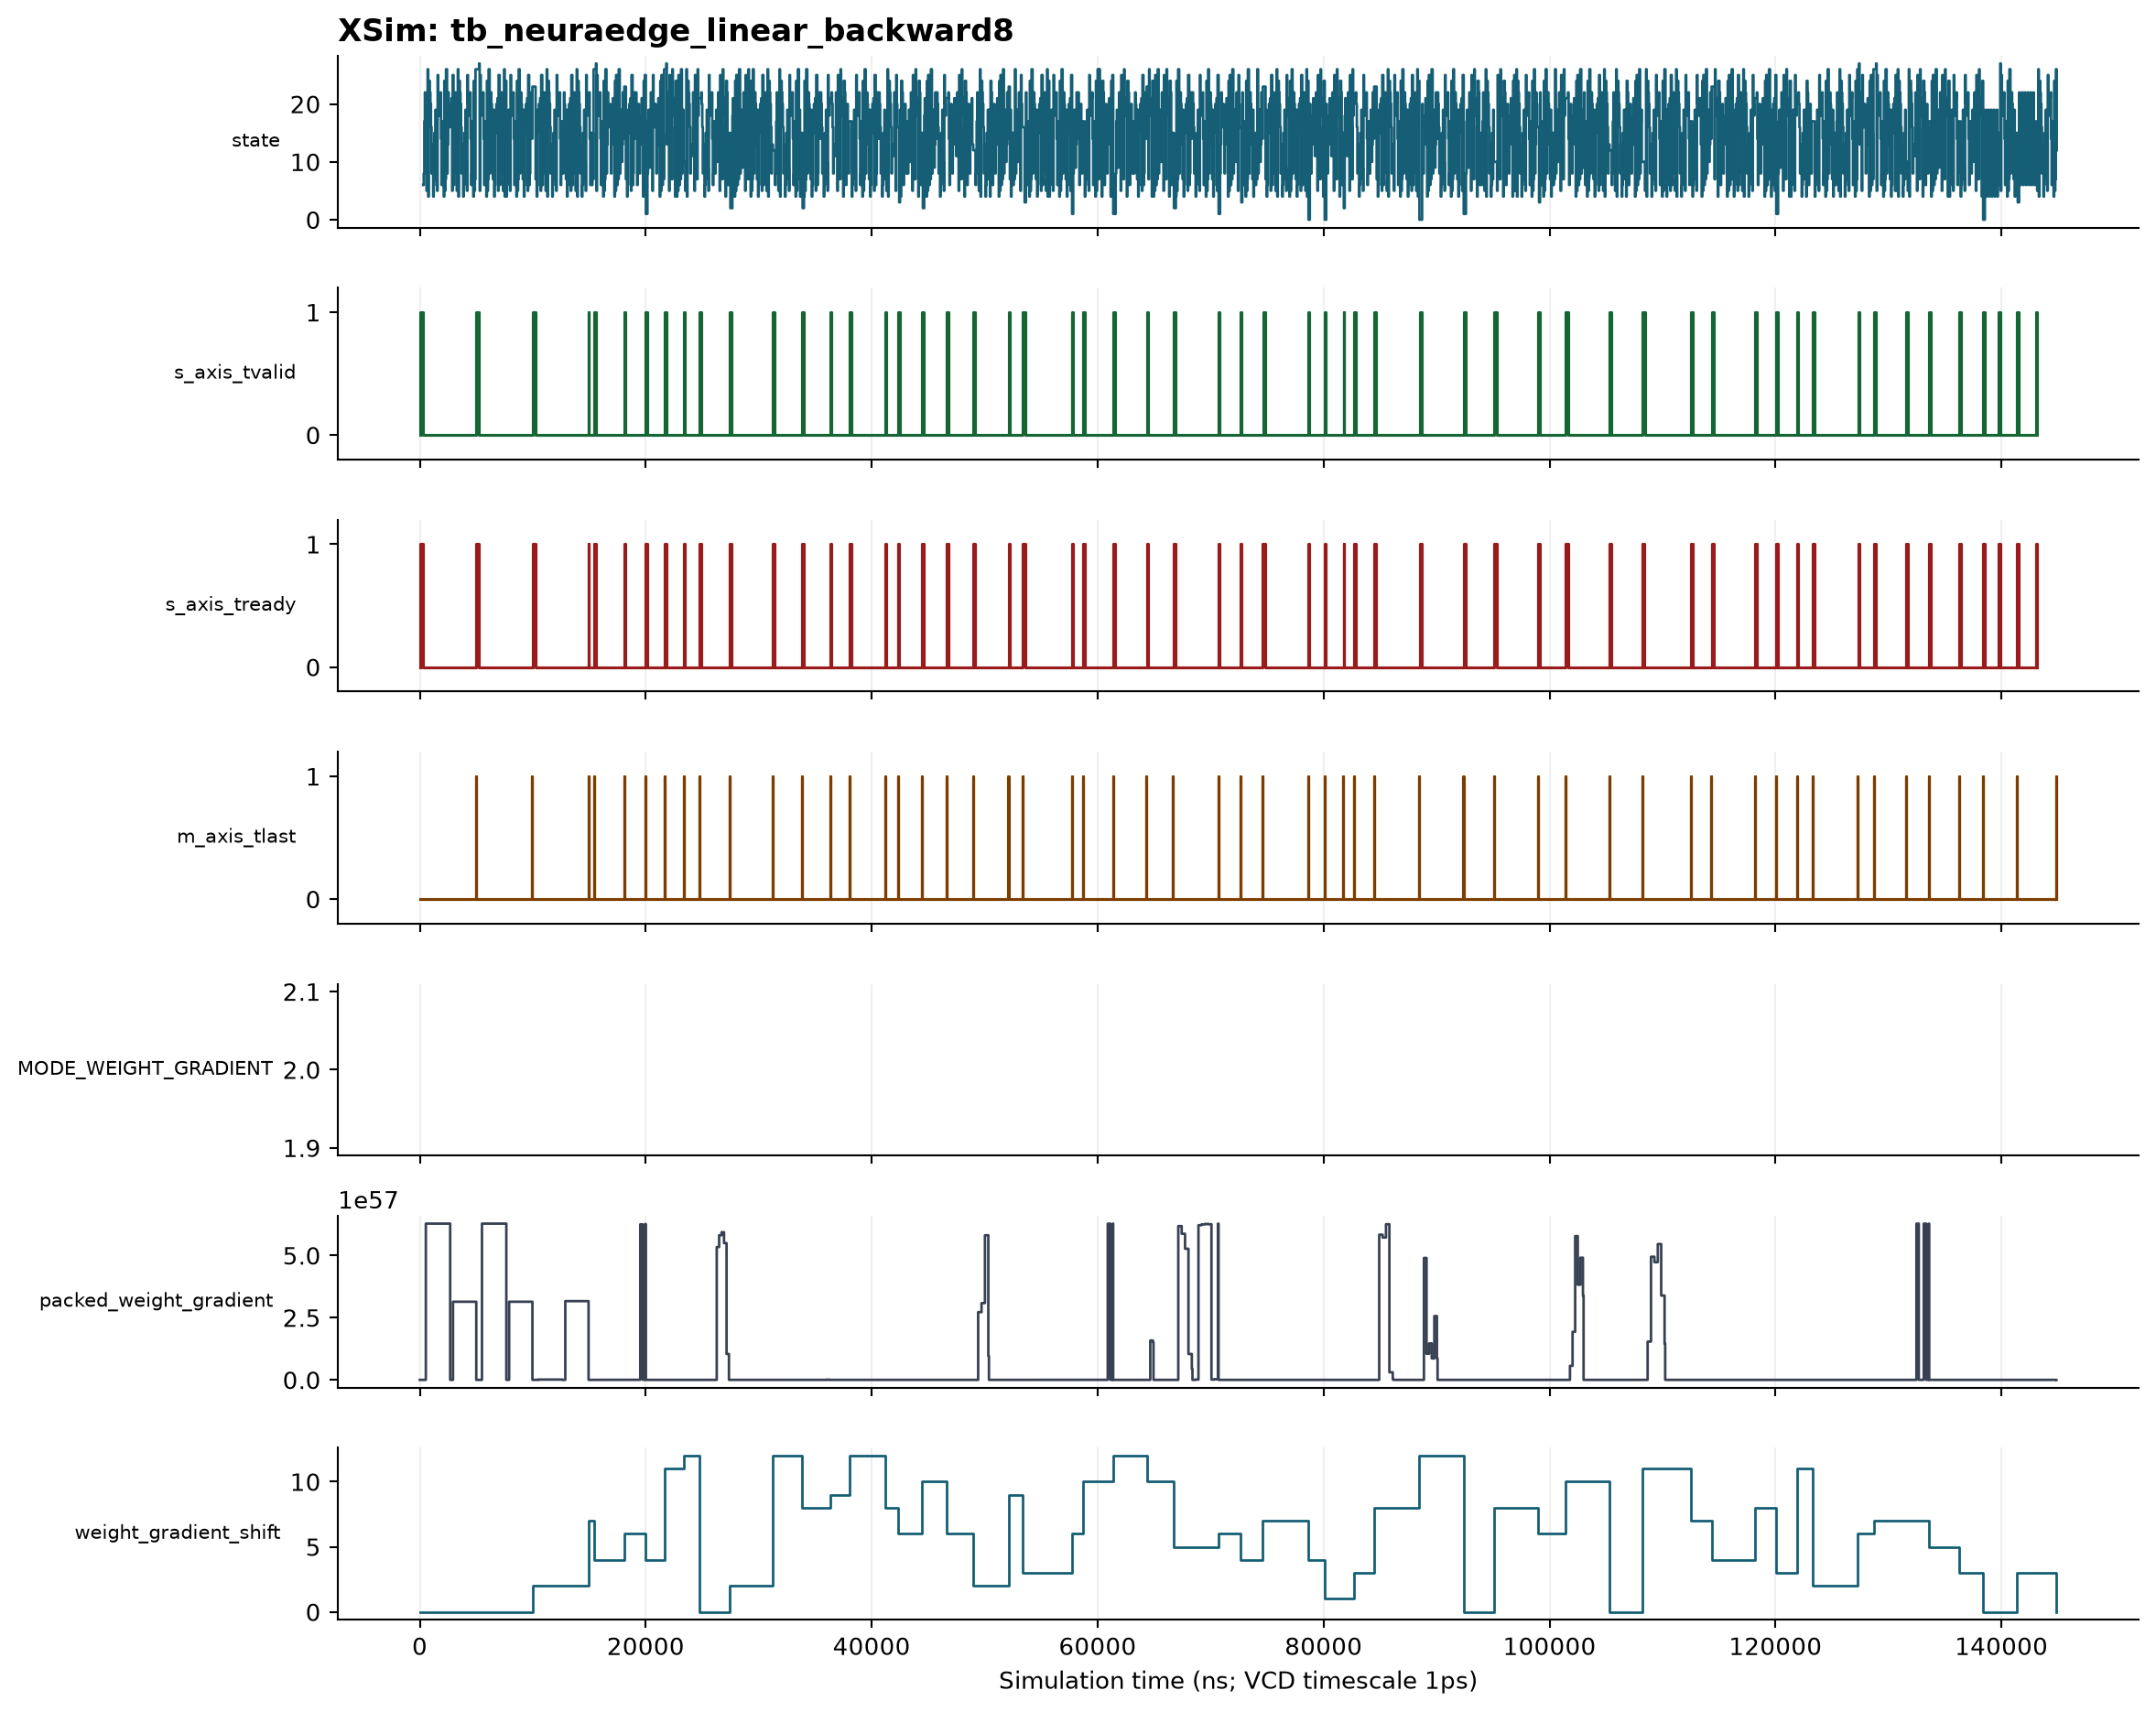
\includegraphics[width=0.98\textwidth,height=0.78\textheight,keepaspectratio]{plots/35_wave_linear_backward8.png}
\end{center}
\clearpage
\section{Waveform: tb\_neuraedge\_sgd\_optimizer8}
\begin{sloppypar}\small\textbf{Evidence:} Vivado 2026.1 XSim VCD,\allowbreak{} requested window 20 us;\allowbreak{} signals: state,\allowbreak{} output\_\allowbreak{}valid,\allowbreak{} output\_\allowbreak{}ready,\allowbreak{} update\_\allowbreak{}count,\allowbreak{} updated\_\allowbreak{}weight\_\allowbreak{}vector,\allowbreak{} weight\_\allowbreak{}decay\_\allowbreak{}q16,\allowbreak{} weight\_\allowbreak{}decay\_\allowbreak{}r,\allowbreak{} weight\_\allowbreak{}vector,\allowbreak{} held\_\allowbreak{}weight\end{sloppypar}
\begin{center}
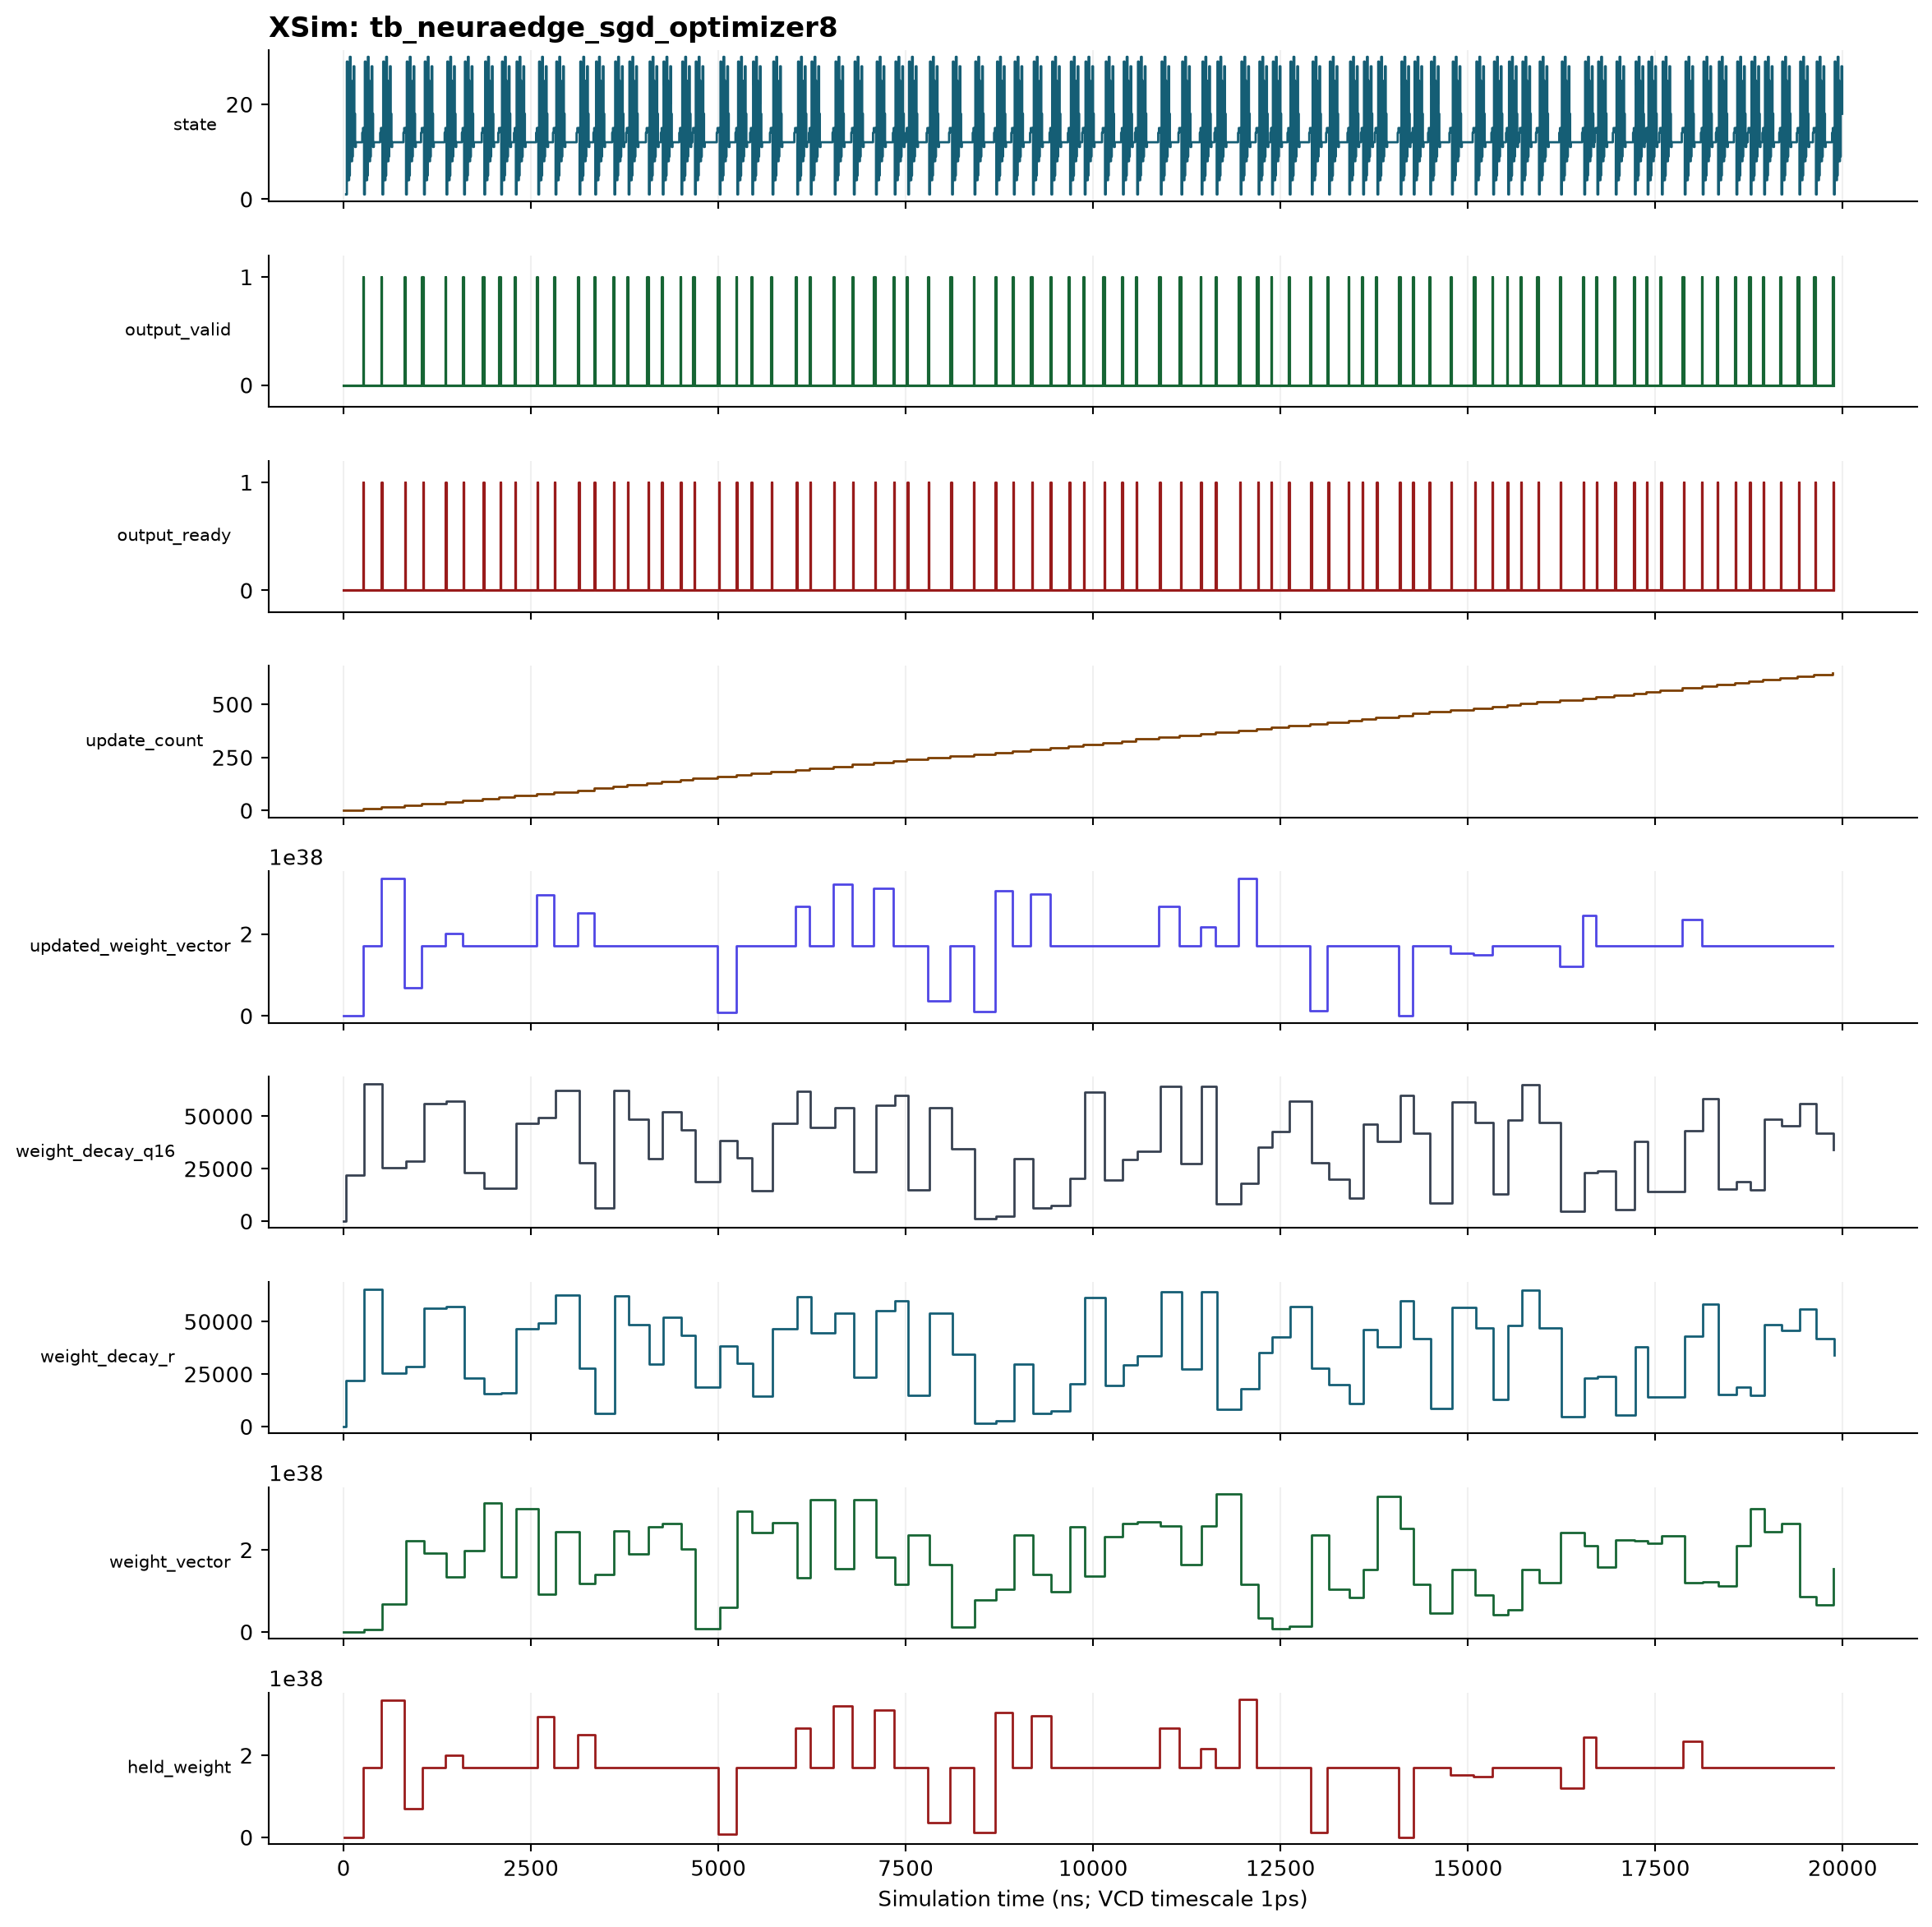
\includegraphics[width=0.98\textwidth,height=0.78\textheight,keepaspectratio]{plots/36_wave_sgd_optimizer8.png}
\end{center}
\clearpage
\section{Waveform: tb\_neuraedge\_activation\_lut8}
\begin{sloppypar}\small\textbf{Evidence:} Vivado 2026.1 XSim VCD,\allowbreak{} requested window 20 us;\allowbreak{} signals: lookup\_\allowbreak{}result\_\allowbreak{}valid\_\allowbreak{}r,\allowbreak{} lookup\_\allowbreak{}result\_\allowbreak{}ready,\allowbreak{} output\_\allowbreak{}valid,\allowbreak{} output\_\allowbreak{}ready,\allowbreak{} result\_\allowbreak{}fifo\_\allowbreak{}count\end{sloppypar}
\begin{center}
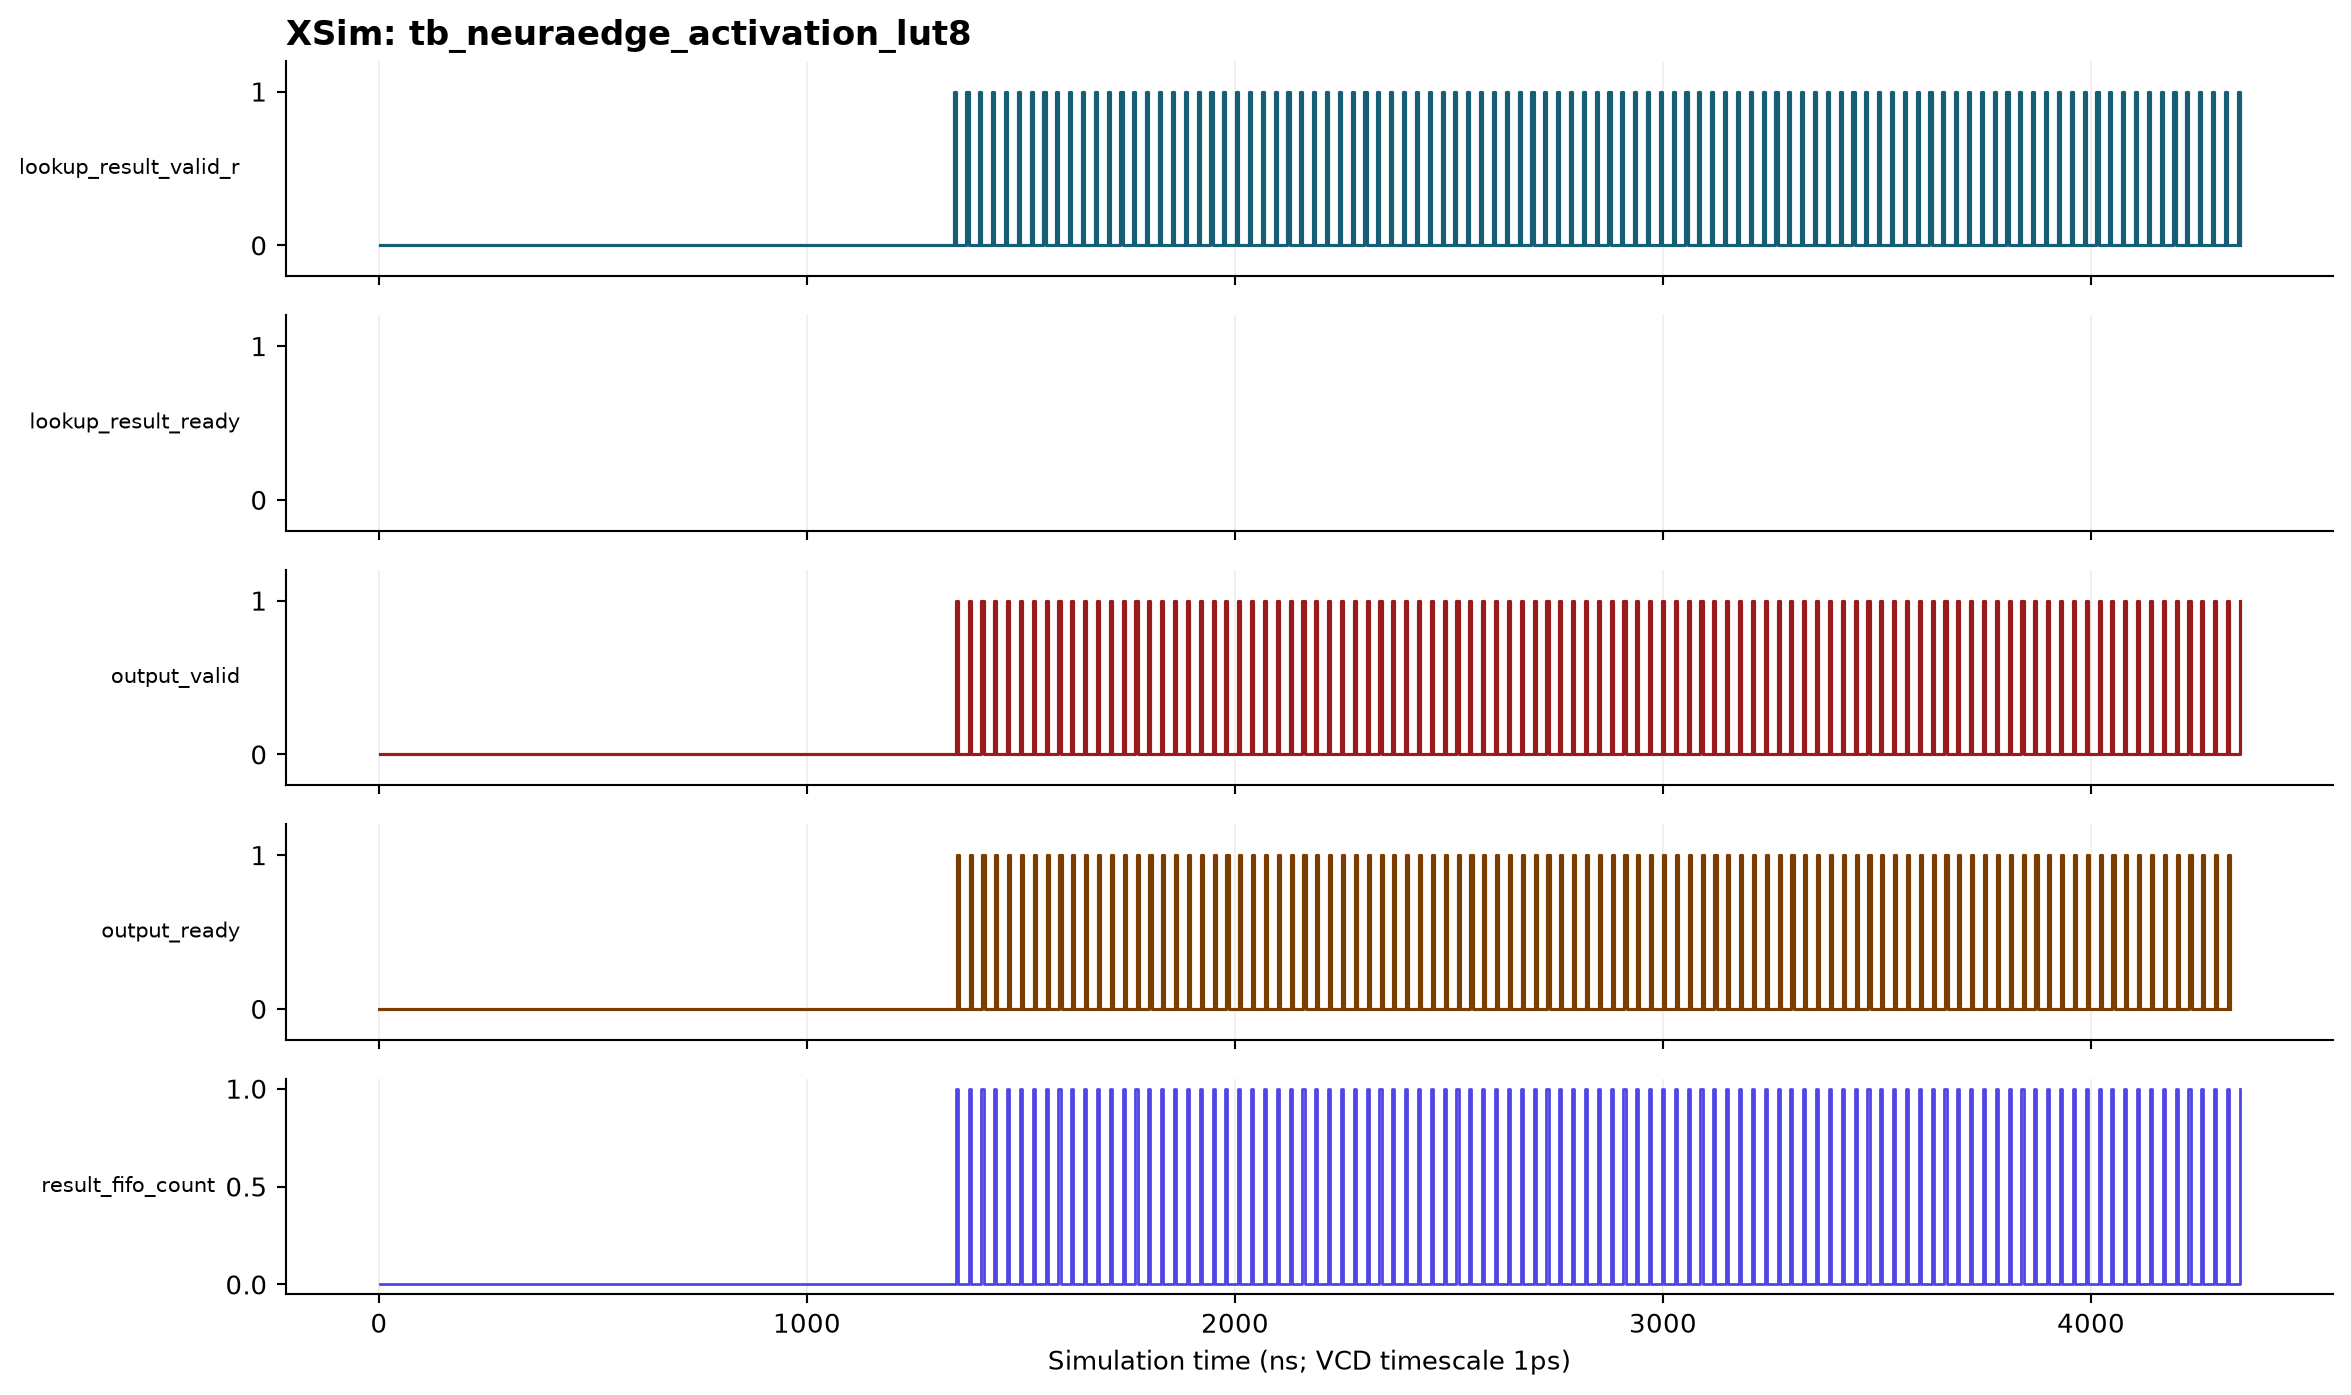
\includegraphics[width=0.98\textwidth,height=0.78\textheight,keepaspectratio]{plots/37_wave_activation_lut8.png}
\end{center}
\clearpage
\section{Waveform: tb\_neuraedge\_universal\_core}
\begin{sloppypar}\small\textbf{Evidence:} Vivado 2026.1 XSim VCD,\allowbreak{} requested window 50 us;\allowbreak{} signals: state,\allowbreak{} command\_\allowbreak{}valid,\allowbreak{} tensor\_\allowbreak{}command\_\allowbreak{}valid,\allowbreak{} s\_\allowbreak{}axis\_\allowbreak{}tvalid,\allowbreak{} s\_\allowbreak{}axis\_\allowbreak{}tready,\allowbreak{} tile\_\allowbreak{}issue\_\allowbreak{}valid,\allowbreak{} issue\_\allowbreak{}valid,\allowbreak{} tile\_\allowbreak{}issue\_\allowbreak{}ready,\allowbreak{} issue\_\allowbreak{}ready,\allowbreak{} ln\_\allowbreak{}result\_\allowbreak{}valid\end{sloppypar}
\begin{center}
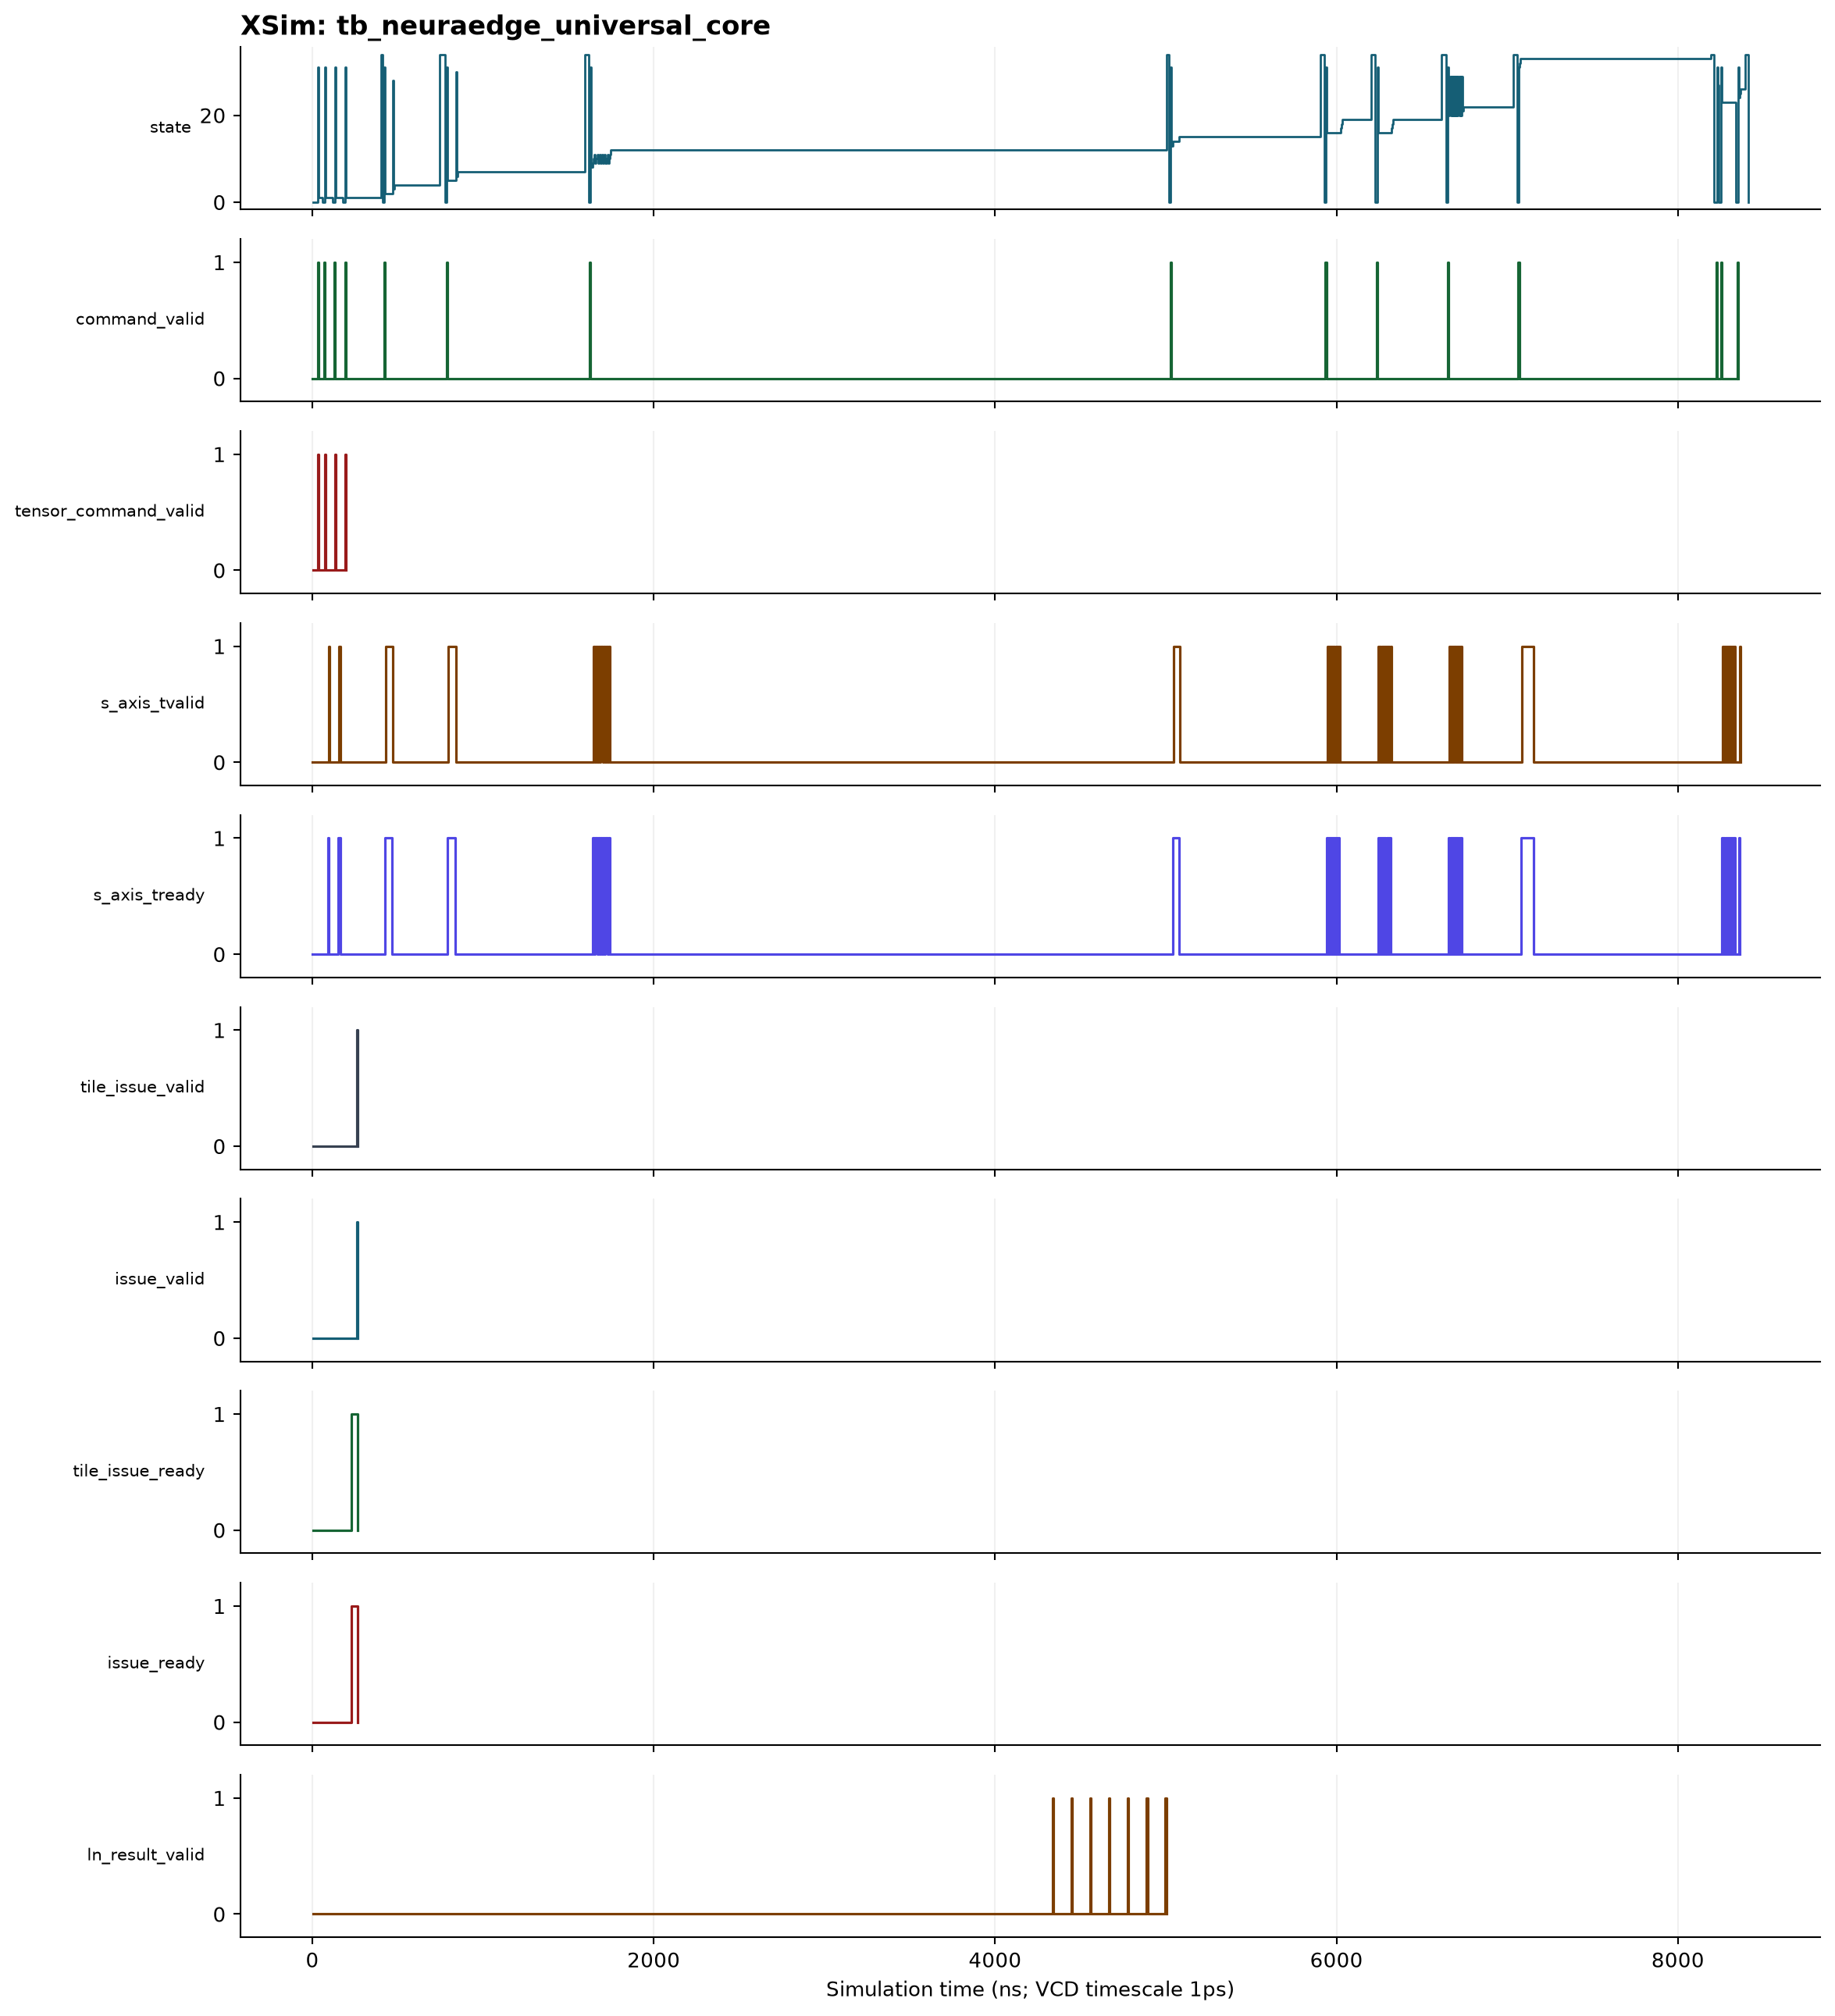
\includegraphics[width=0.98\textwidth,height=0.78\textheight,keepaspectratio]{plots/38_wave_universal_core.png}
\end{center}
\clearpage
\section{Waveform: tb\_neuraedge\_descriptor\_sequencer}
\begin{sloppypar}\small\textbf{Evidence:} Vivado 2026.1 XSim VCD,\allowbreak{} requested window 2 us;\allowbreak{} signals: program\_\allowbreak{}active,\allowbreak{} program\_\allowbreak{}done,\allowbreak{} program\_\allowbreak{}error,\allowbreak{} state,\allowbreak{} core\_\allowbreak{}command\_\allowbreak{}valid,\allowbreak{} input\_\allowbreak{}fifo\_\allowbreak{}count\_\allowbreak{}r,\allowbreak{} s\_\allowbreak{}axis\_\allowbreak{}tvalid,\allowbreak{} s\_\allowbreak{}axis\_\allowbreak{}tready,\allowbreak{} core\_\allowbreak{}s\_\allowbreak{}valid,\allowbreak{} core\_\allowbreak{}s\_\allowbreak{}ready\end{sloppypar}
\begin{center}
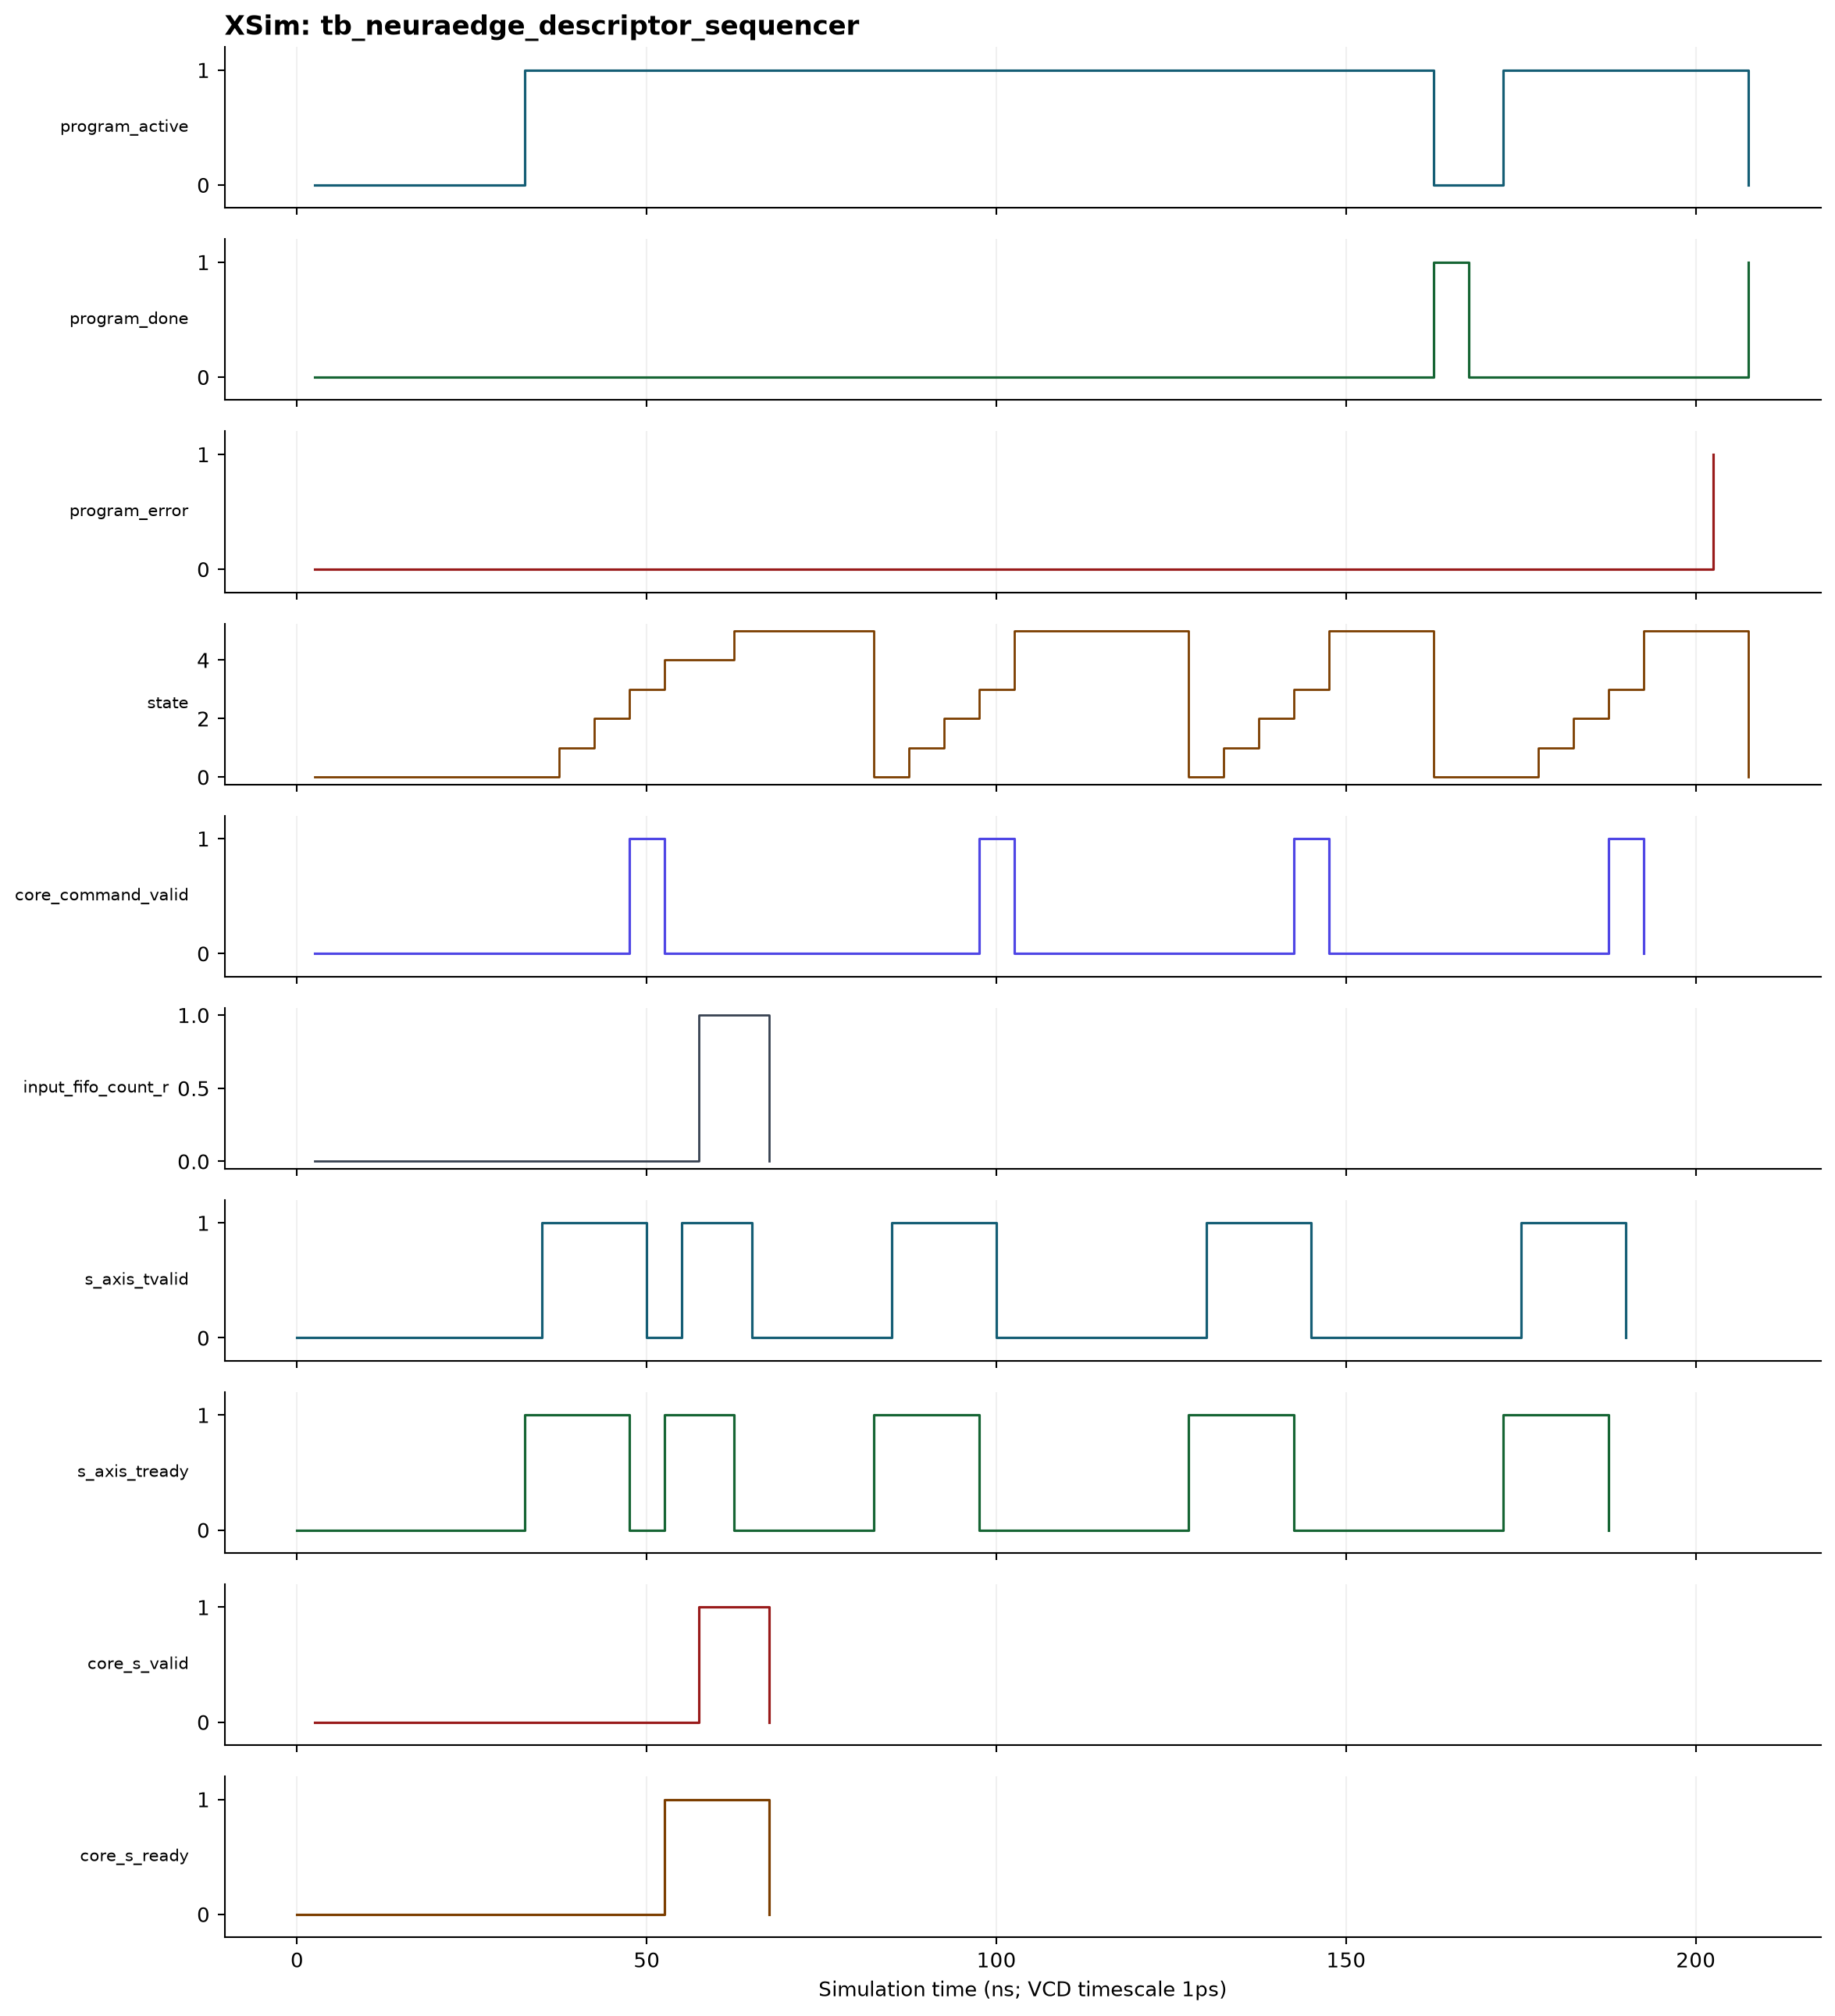
\includegraphics[width=0.98\textwidth,height=0.78\textheight,keepaspectratio]{plots/39_wave_descriptor_sequencer.png}
\end{center}
\clearpage
\section{Waveform: tb\_neuraedge\_pynq\_descriptor}
\begin{sloppypar}\small\textbf{Evidence:} Vivado 2026.1 XSim VCD,\allowbreak{} requested window 2 us;\allowbreak{} signals: program\_\allowbreak{}active,\allowbreak{} program\_\allowbreak{}done,\allowbreak{} program\_\allowbreak{}error,\allowbreak{} state,\allowbreak{} sequencer\_\allowbreak{}core\_\allowbreak{}command\_\allowbreak{}valid,\allowbreak{} command\_\allowbreak{}valid,\allowbreak{} tensor\_\allowbreak{}command\_\allowbreak{}valid,\allowbreak{} core\_\allowbreak{}command\_\allowbreak{}valid,\allowbreak{} input\_\allowbreak{}fifo\_\allowbreak{}count,\allowbreak{} input\_\allowbreak{}fifo\_\allowbreak{}count\_\allowbreak{}r\end{sloppypar}
\begin{center}
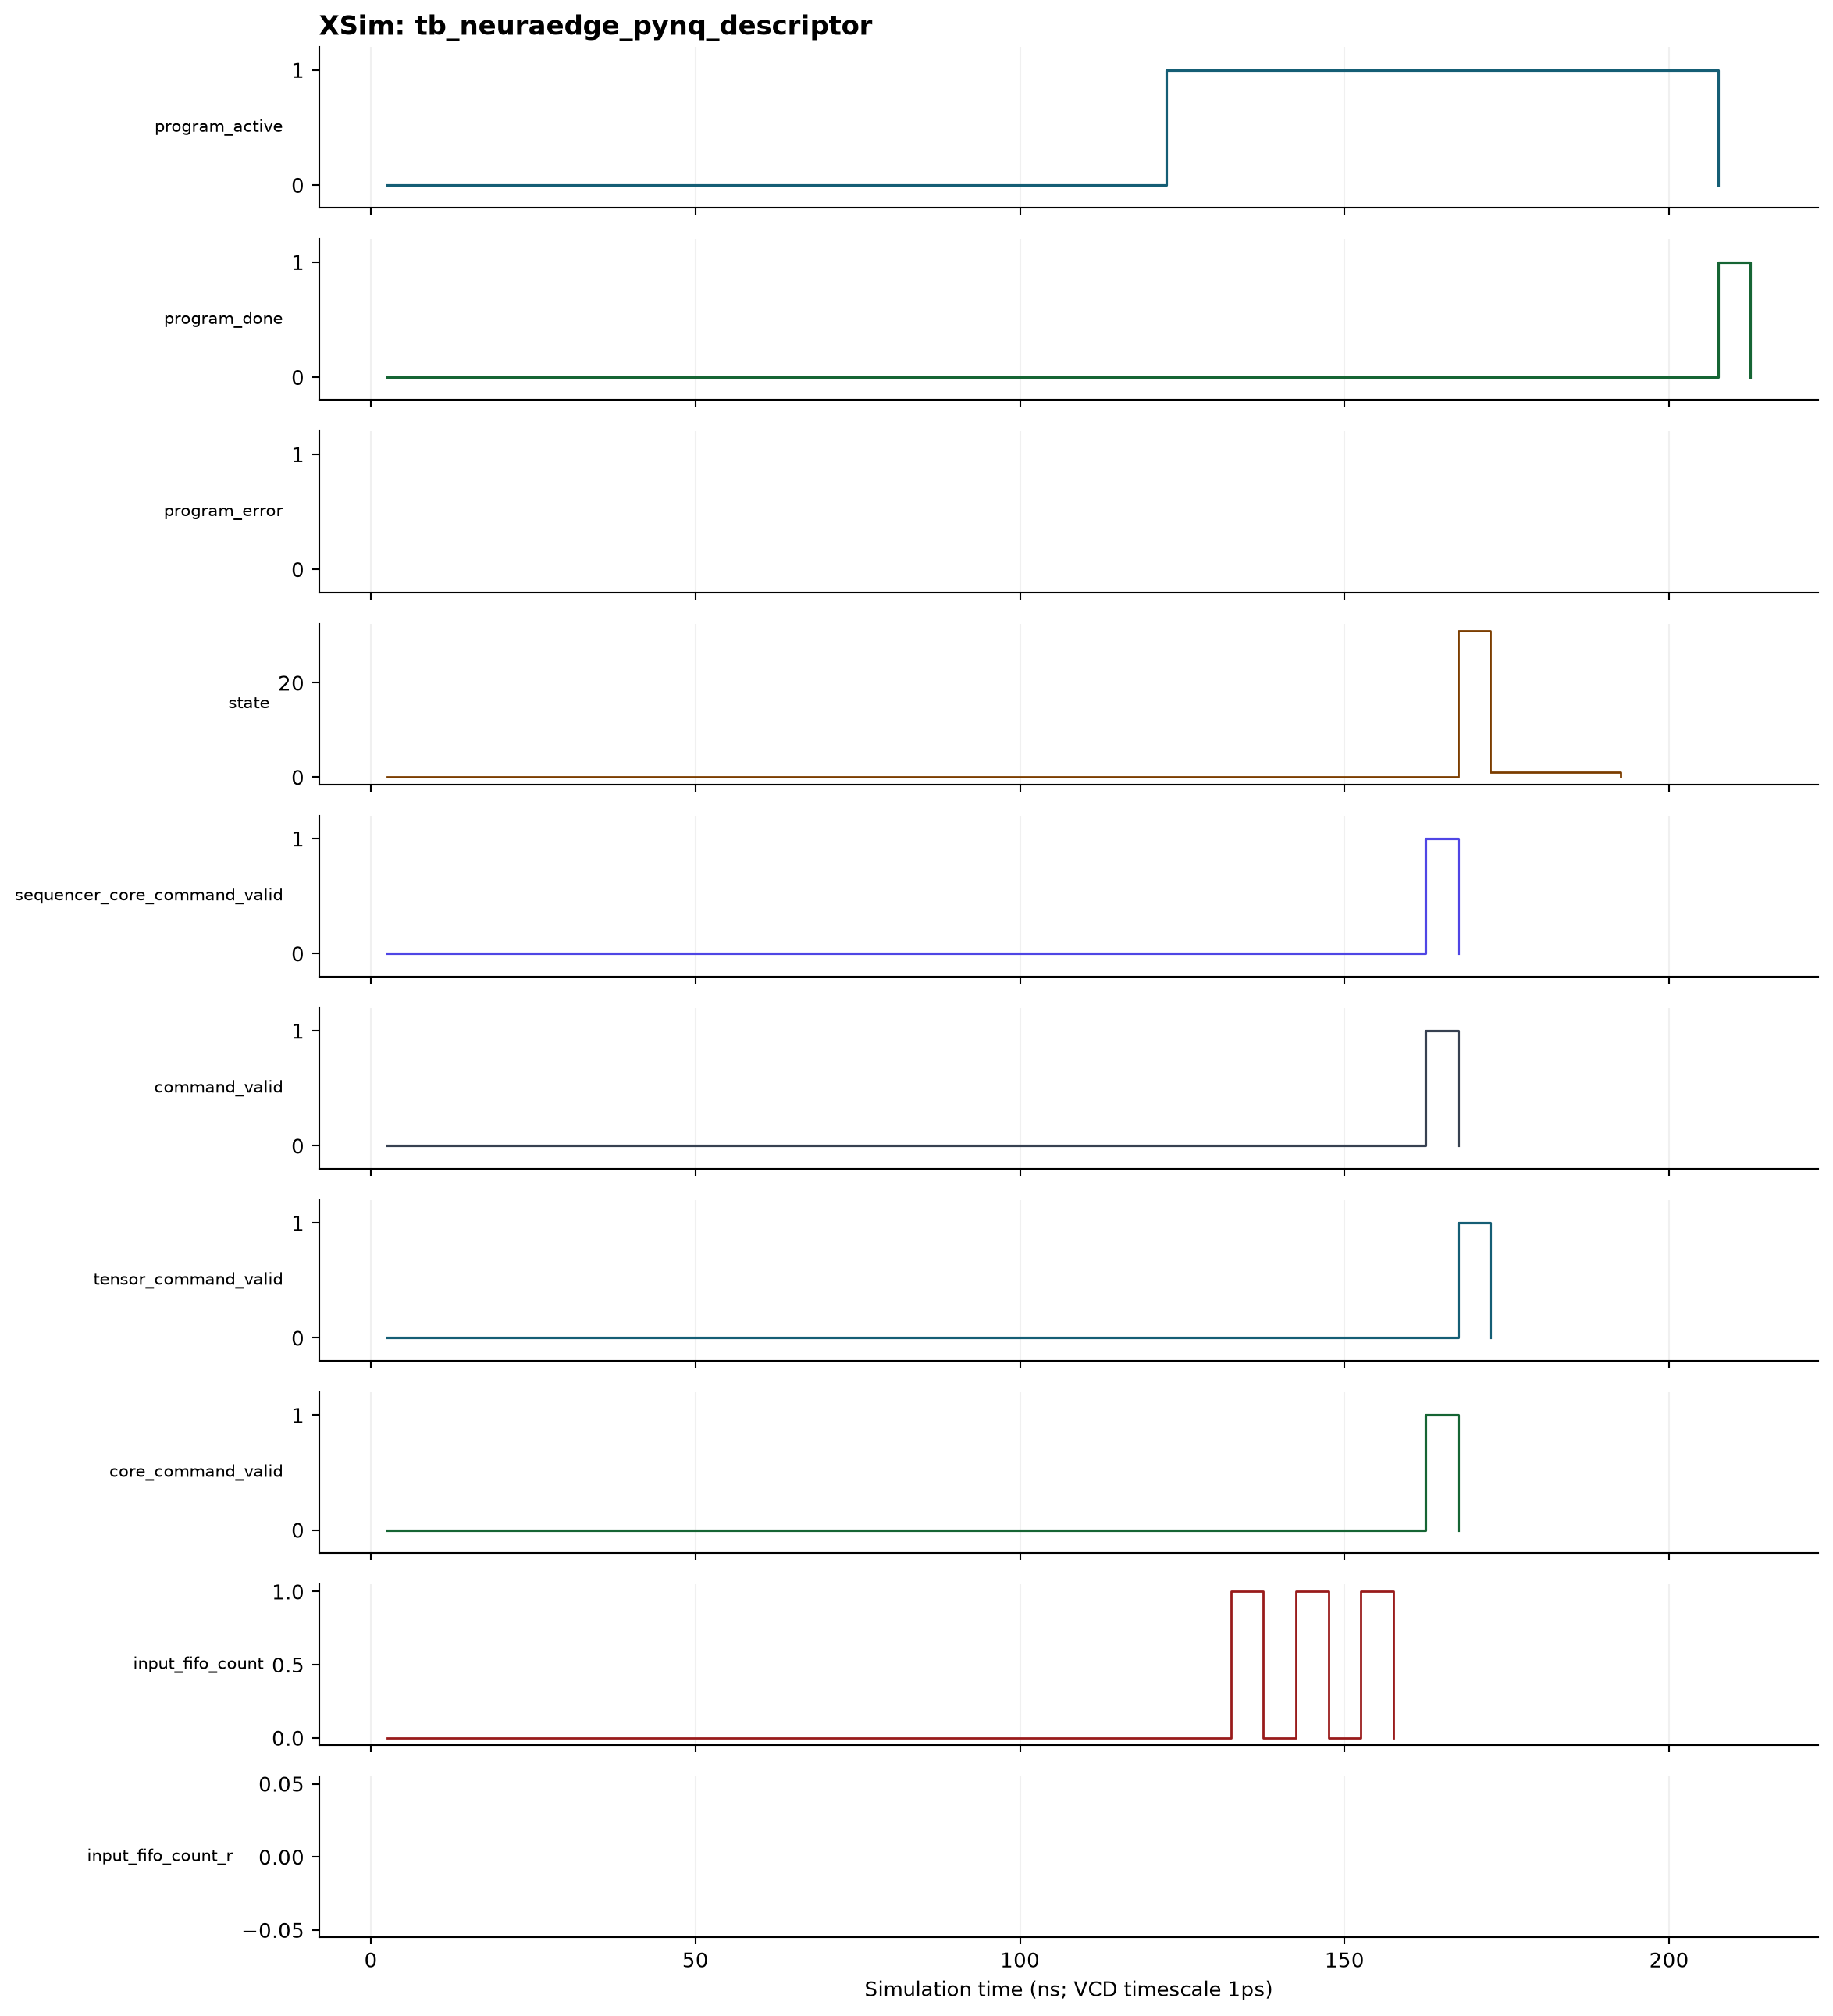
\includegraphics[width=0.98\textwidth,height=0.78\textheight,keepaspectratio]{plots/40_wave_pynq_descriptor.png}
\end{center}
\clearpage
\section{Waveform: tb\_neuraedge\_pynq\_axi\_top}
\begin{sloppypar}\small\textbf{Evidence:} Vivado 2026.1 XSim VCD,\allowbreak{} requested window 5 us;\allowbreak{} signals: program\_\allowbreak{}active,\allowbreak{} program\_\allowbreak{}done,\allowbreak{} program\_\allowbreak{}error,\allowbreak{} state,\allowbreak{} sequencer\_\allowbreak{}core\_\allowbreak{}command\_\allowbreak{}valid,\allowbreak{} command\_\allowbreak{}valid,\allowbreak{} tensor\_\allowbreak{}command\_\allowbreak{}valid,\allowbreak{} core\_\allowbreak{}command\_\allowbreak{}valid,\allowbreak{} input\_\allowbreak{}fifo\_\allowbreak{}count,\allowbreak{} input\_\allowbreak{}fifo\_\allowbreak{}count\_\allowbreak{}r\end{sloppypar}
\begin{center}
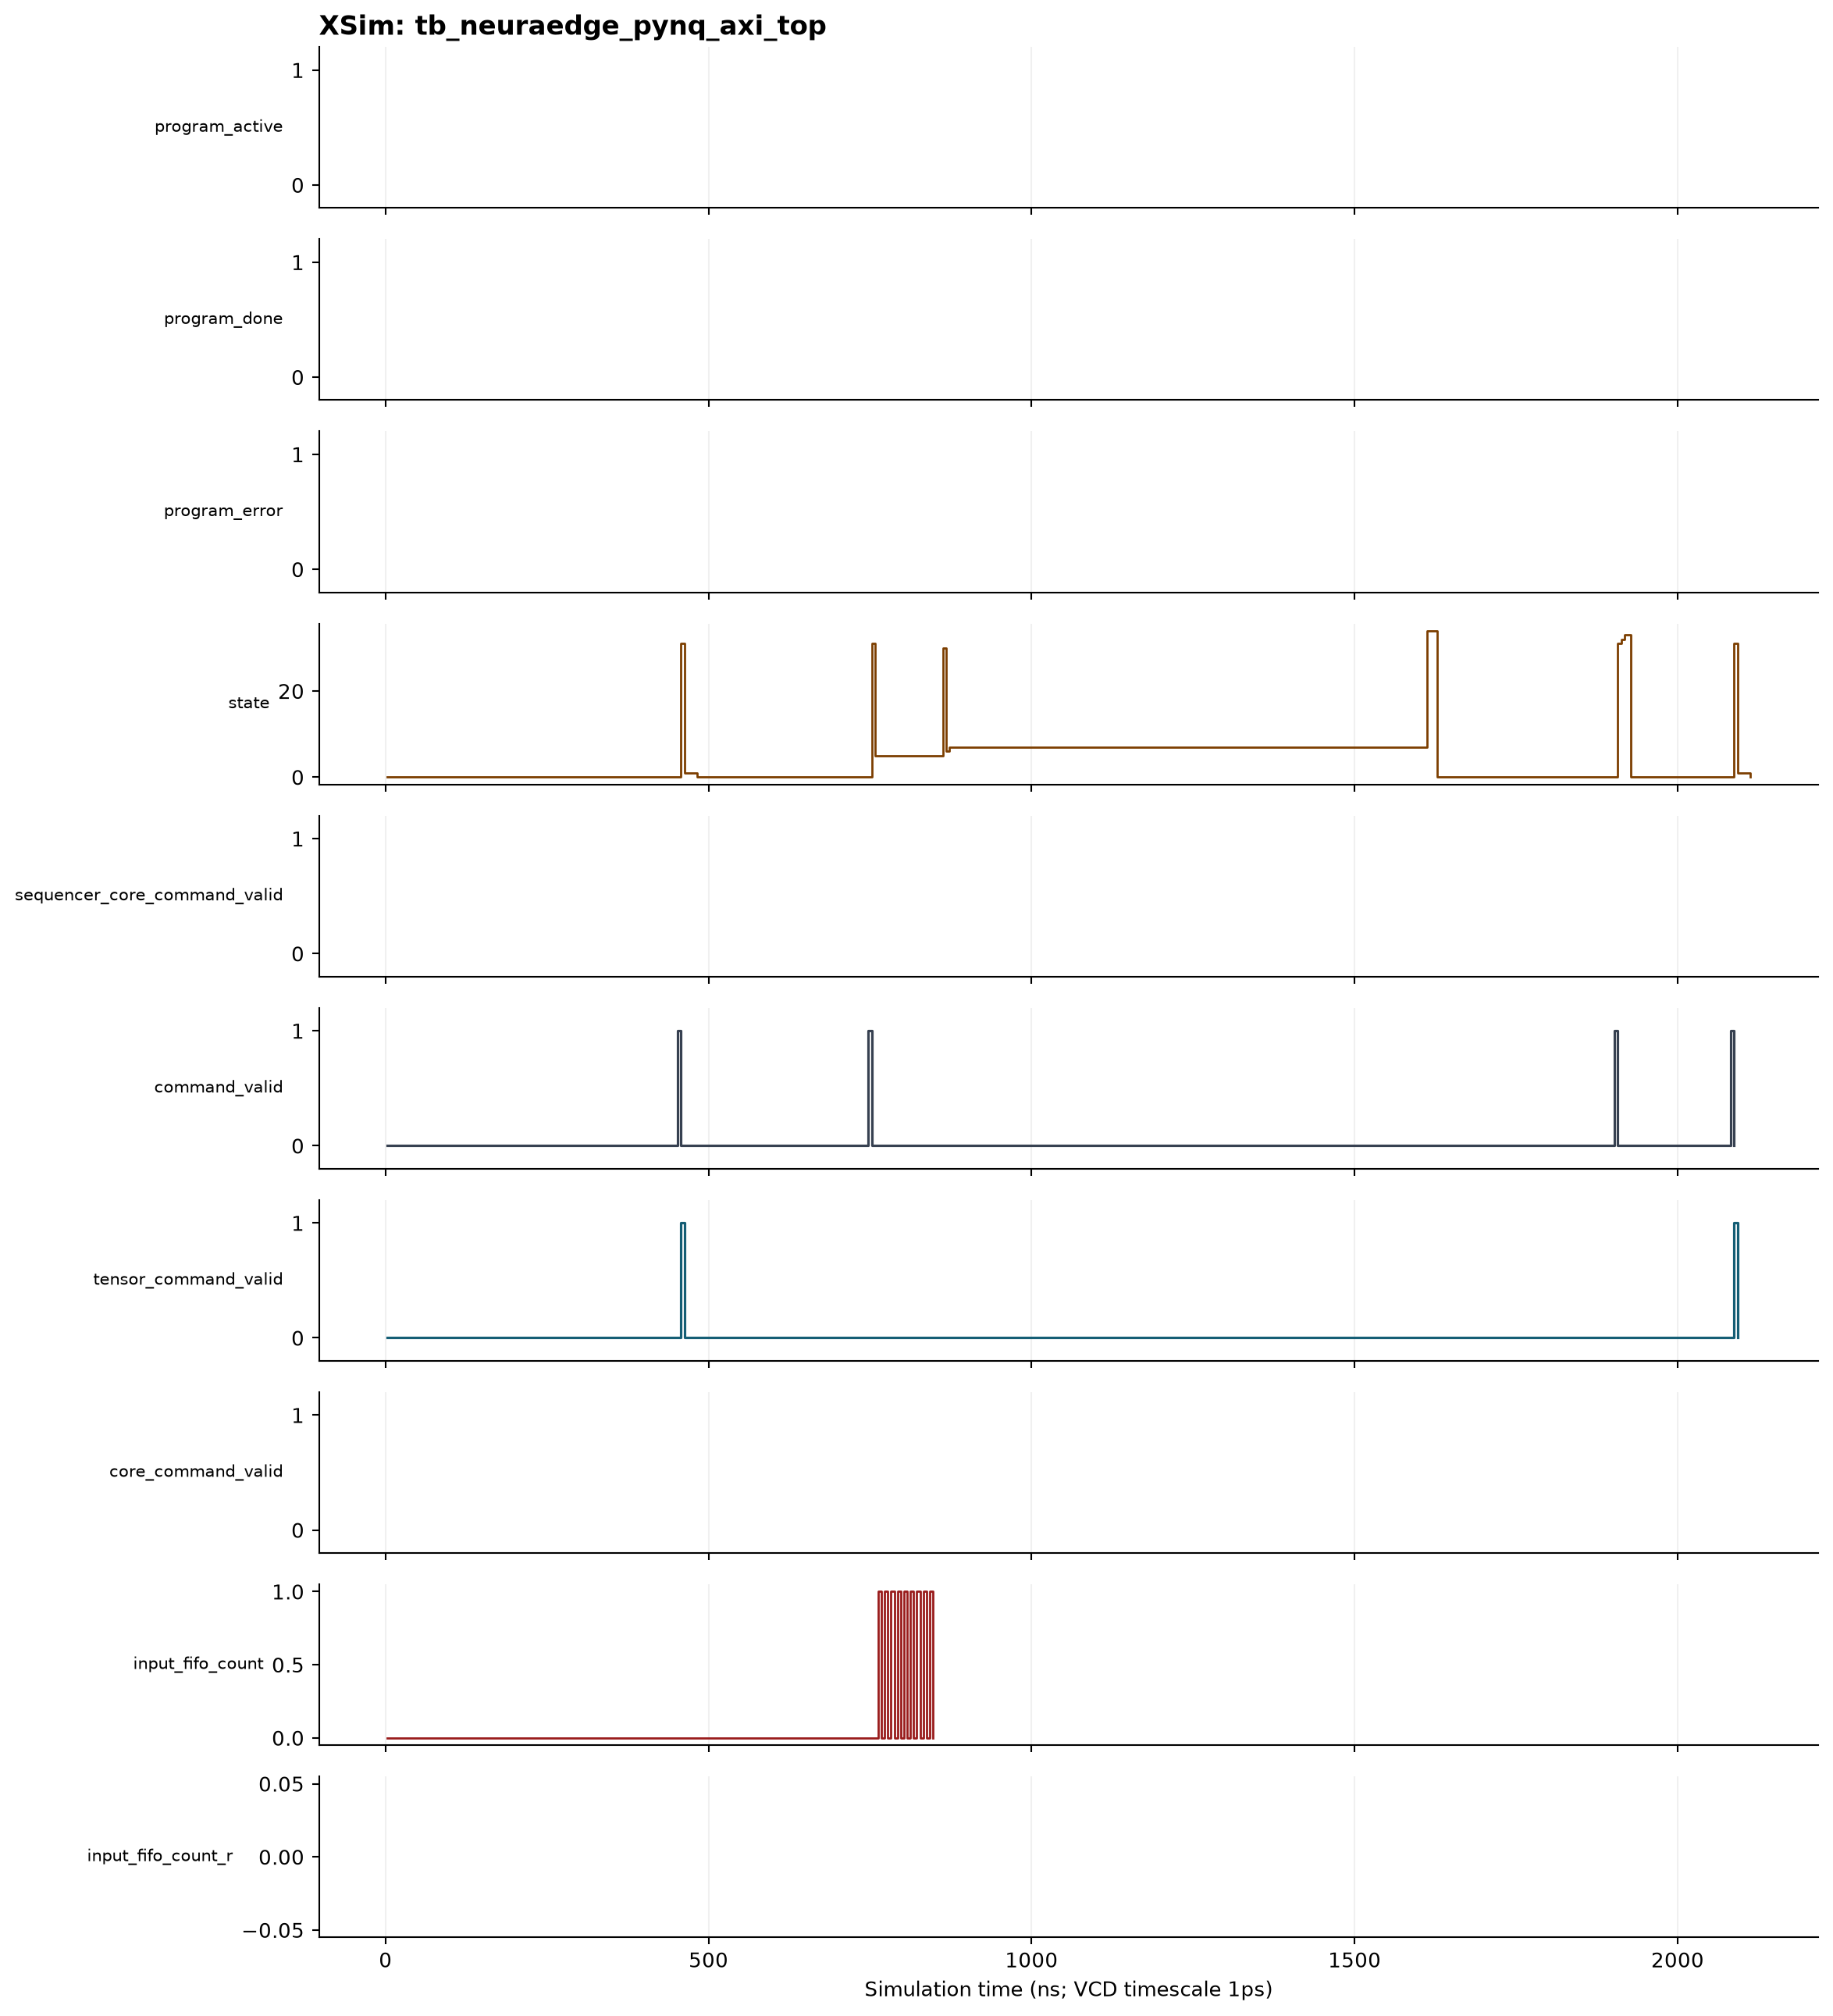
\includegraphics[width=0.98\textwidth,height=0.78\textheight,keepaspectratio]{plots/41_wave_pynq_axi_top.png}
\end{center}
\clearpage
\section{Routed timing by clock domain}
\begin{sloppypar}\small\textbf{Evidence:} C:\textbackslash{}\allowbreak{}Users\textbackslash{}\allowbreak{}Ross\textbackslash{}\allowbreak{}Downloads\textbackslash{}\allowbreak{}neuraedge--main\textbackslash{}\allowbreak{}neuraedge--main\textbackslash{}\allowbreak{}neuraedge\_\allowbreak{}universal\textbackslash{}\allowbreak{}outputs\textbackslash{}\allowbreak{}pynq\_\allowbreak{}full\textbackslash{}\allowbreak{}full\_\allowbreak{}routed\_\allowbreak{}timing\_\allowbreak{}summary.rpt\end{sloppypar}
\begin{center}
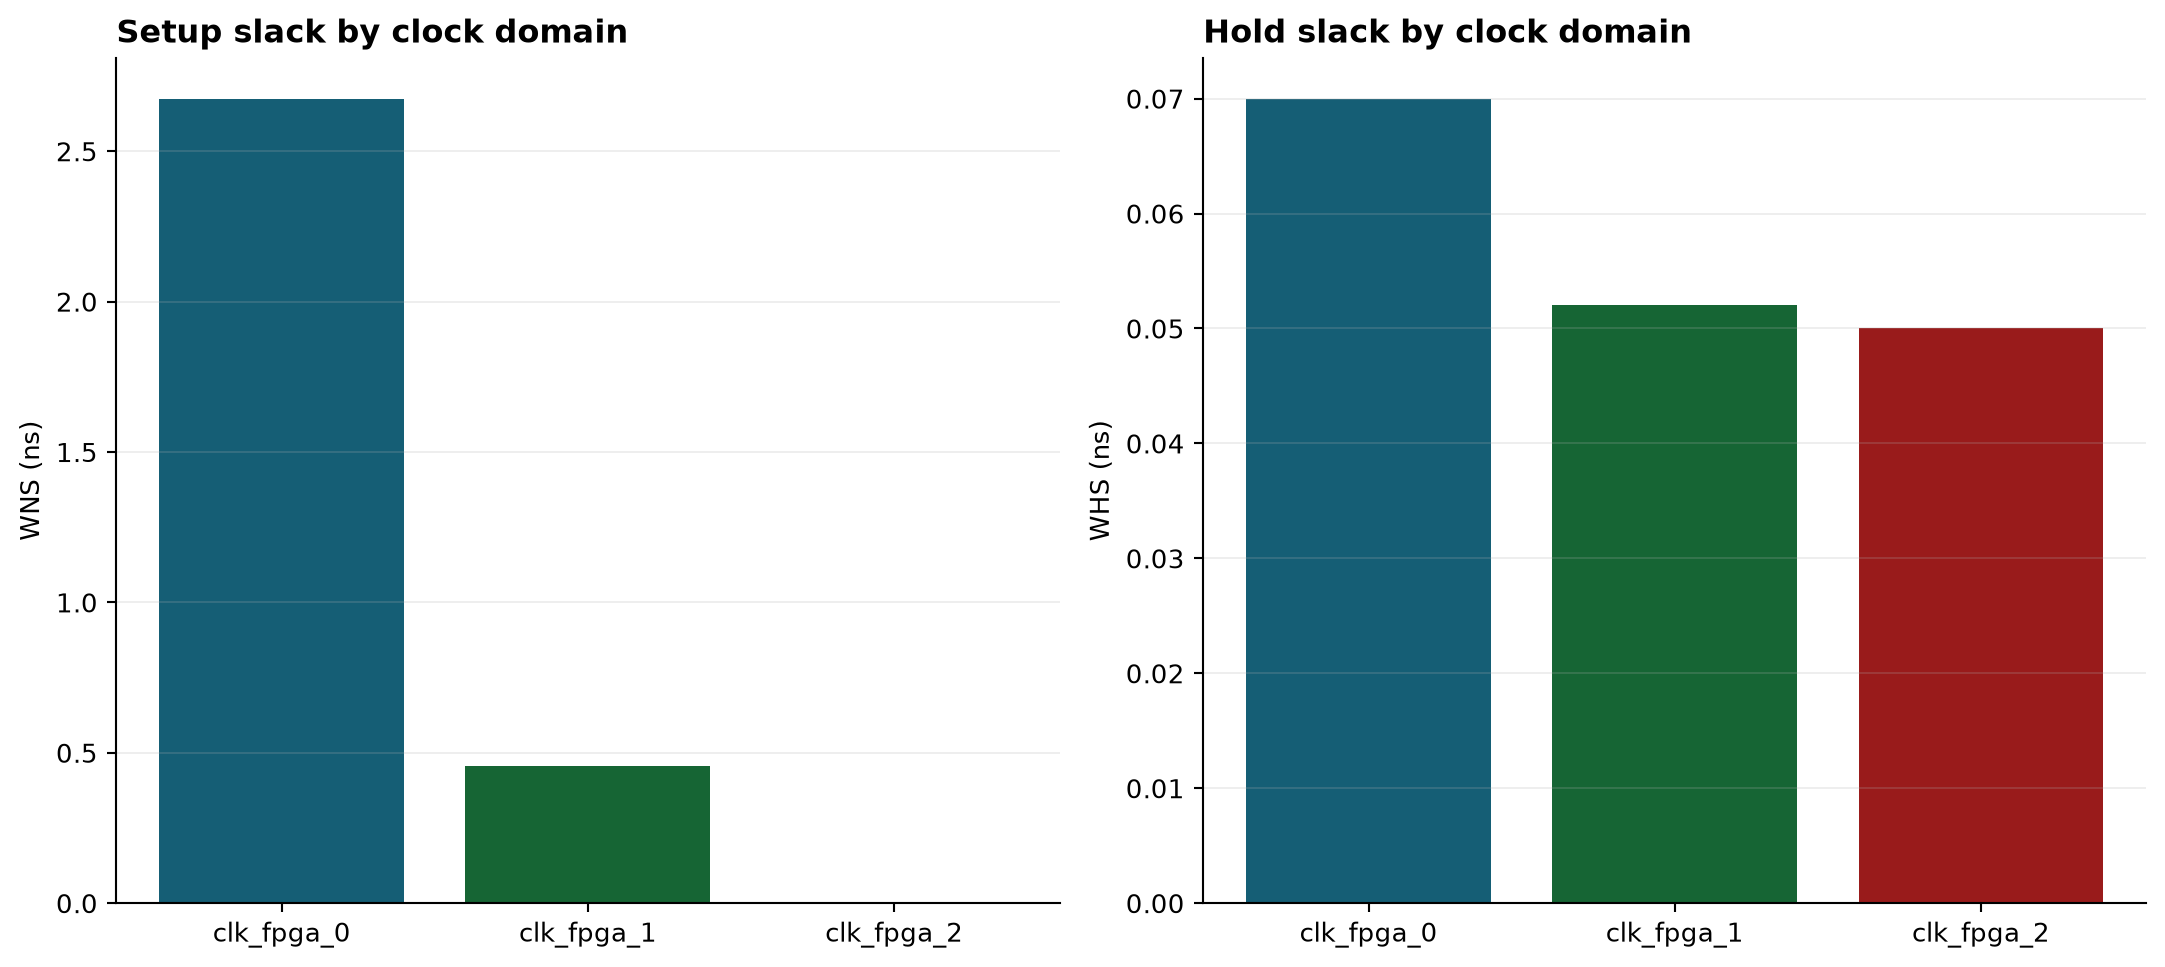
\includegraphics[width=0.98\textwidth,height=0.78\textheight,keepaspectratio]{plots/42_clock_domain_timing.png}
\end{center}
\clearpage
\section{Full PYNQ routed resource utilization}
\begin{sloppypar}\small\textbf{Evidence:} C:\textbackslash{}\allowbreak{}Users\textbackslash{}\allowbreak{}Ross\textbackslash{}\allowbreak{}Downloads\textbackslash{}\allowbreak{}neuraedge--main\textbackslash{}\allowbreak{}neuraedge--main\textbackslash{}\allowbreak{}neuraedge\_\allowbreak{}universal\textbackslash{}\allowbreak{}outputs\textbackslash{}\allowbreak{}pynq\_\allowbreak{}full\textbackslash{}\allowbreak{}full\_\allowbreak{}routed\_\allowbreak{}utilization\_\allowbreak{}hierarchical.rpt\end{sloppypar}
\begin{center}
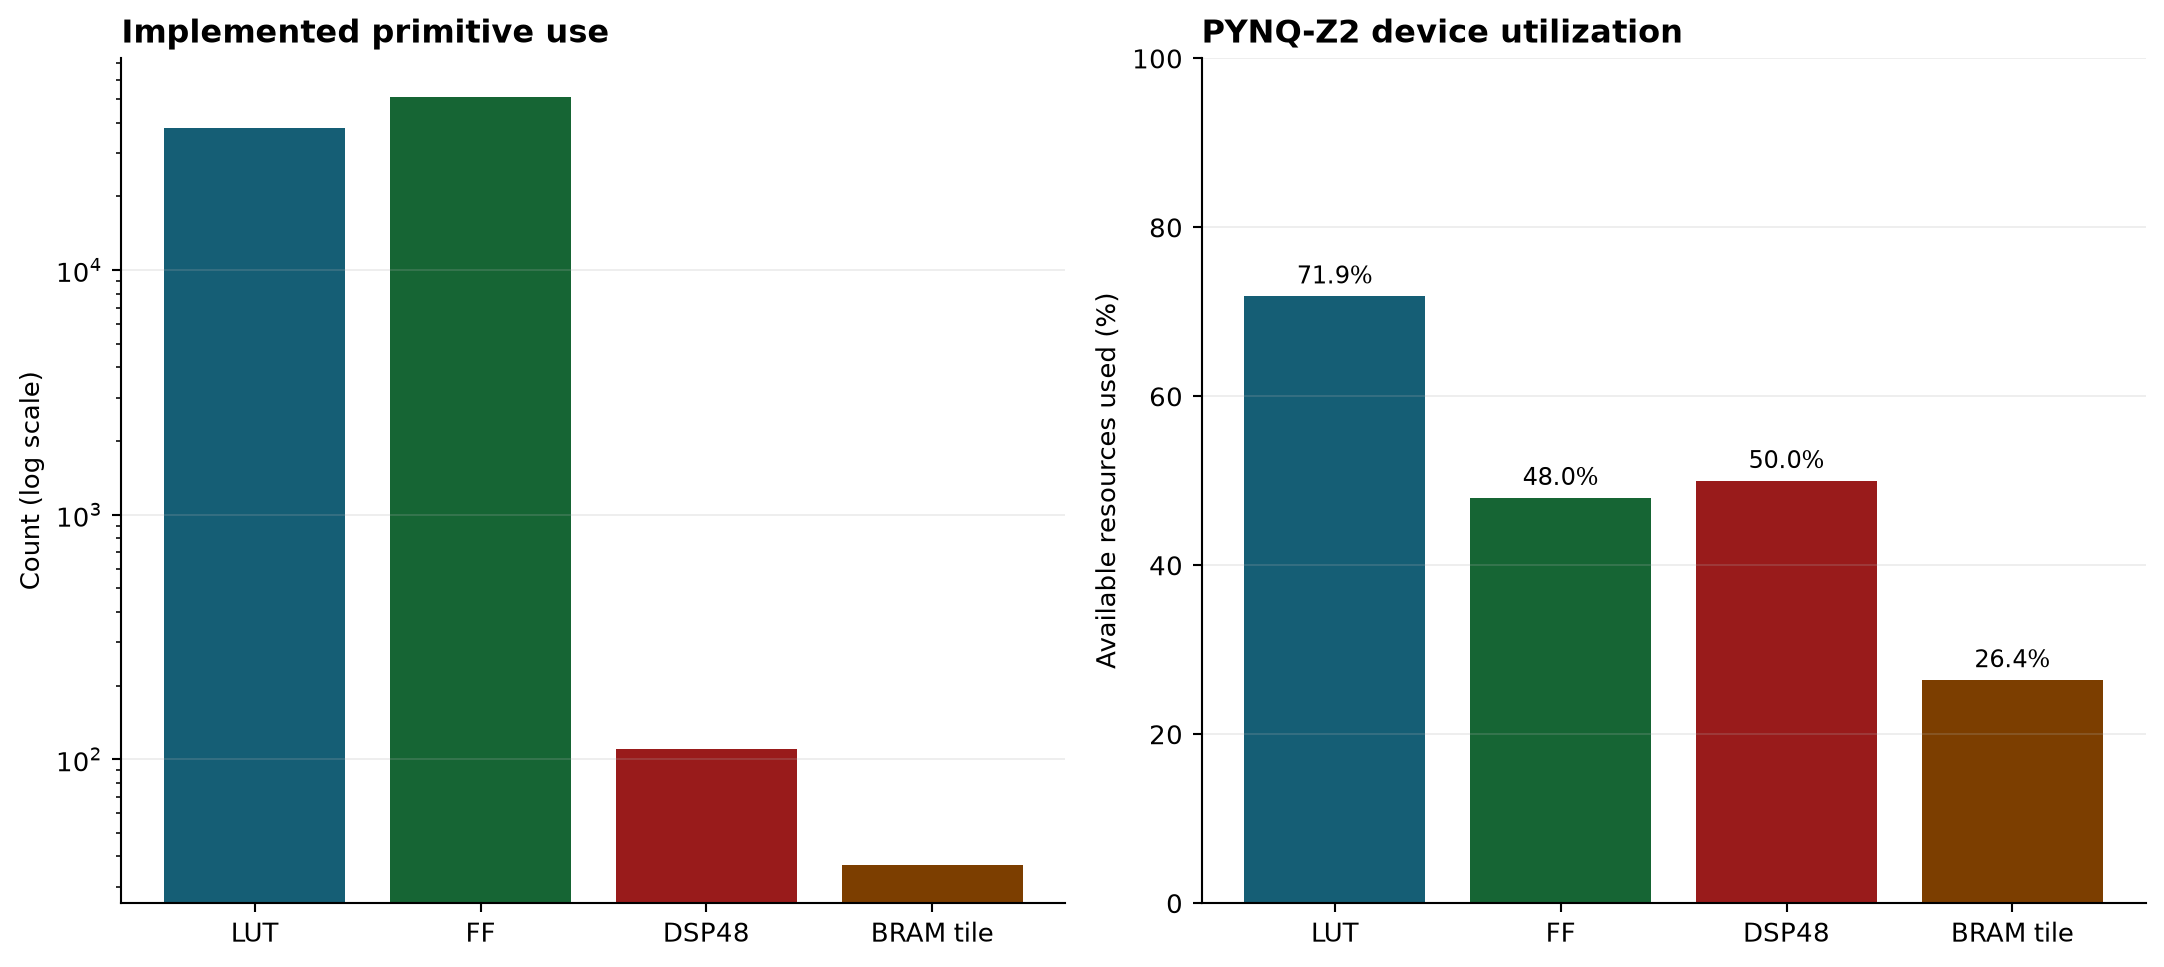
\includegraphics[width=0.98\textwidth,height=0.78\textheight,keepaspectratio]{plots/43_full_routed_resources.png}
\end{center}
\clearpage
\section{Resource use by full-system hierarchy}
\begin{sloppypar}\small\textbf{Evidence:} C:\textbackslash{}\allowbreak{}Users\textbackslash{}\allowbreak{}Ross\textbackslash{}\allowbreak{}Downloads\textbackslash{}\allowbreak{}neuraedge--main\textbackslash{}\allowbreak{}neuraedge--main\textbackslash{}\allowbreak{}neuraedge\_\allowbreak{}universal\textbackslash{}\allowbreak{}outputs\textbackslash{}\allowbreak{}pynq\_\allowbreak{}full\textbackslash{}\allowbreak{}full\_\allowbreak{}routed\_\allowbreak{}utilization\_\allowbreak{}hierarchical.rpt\end{sloppypar}
\begin{center}
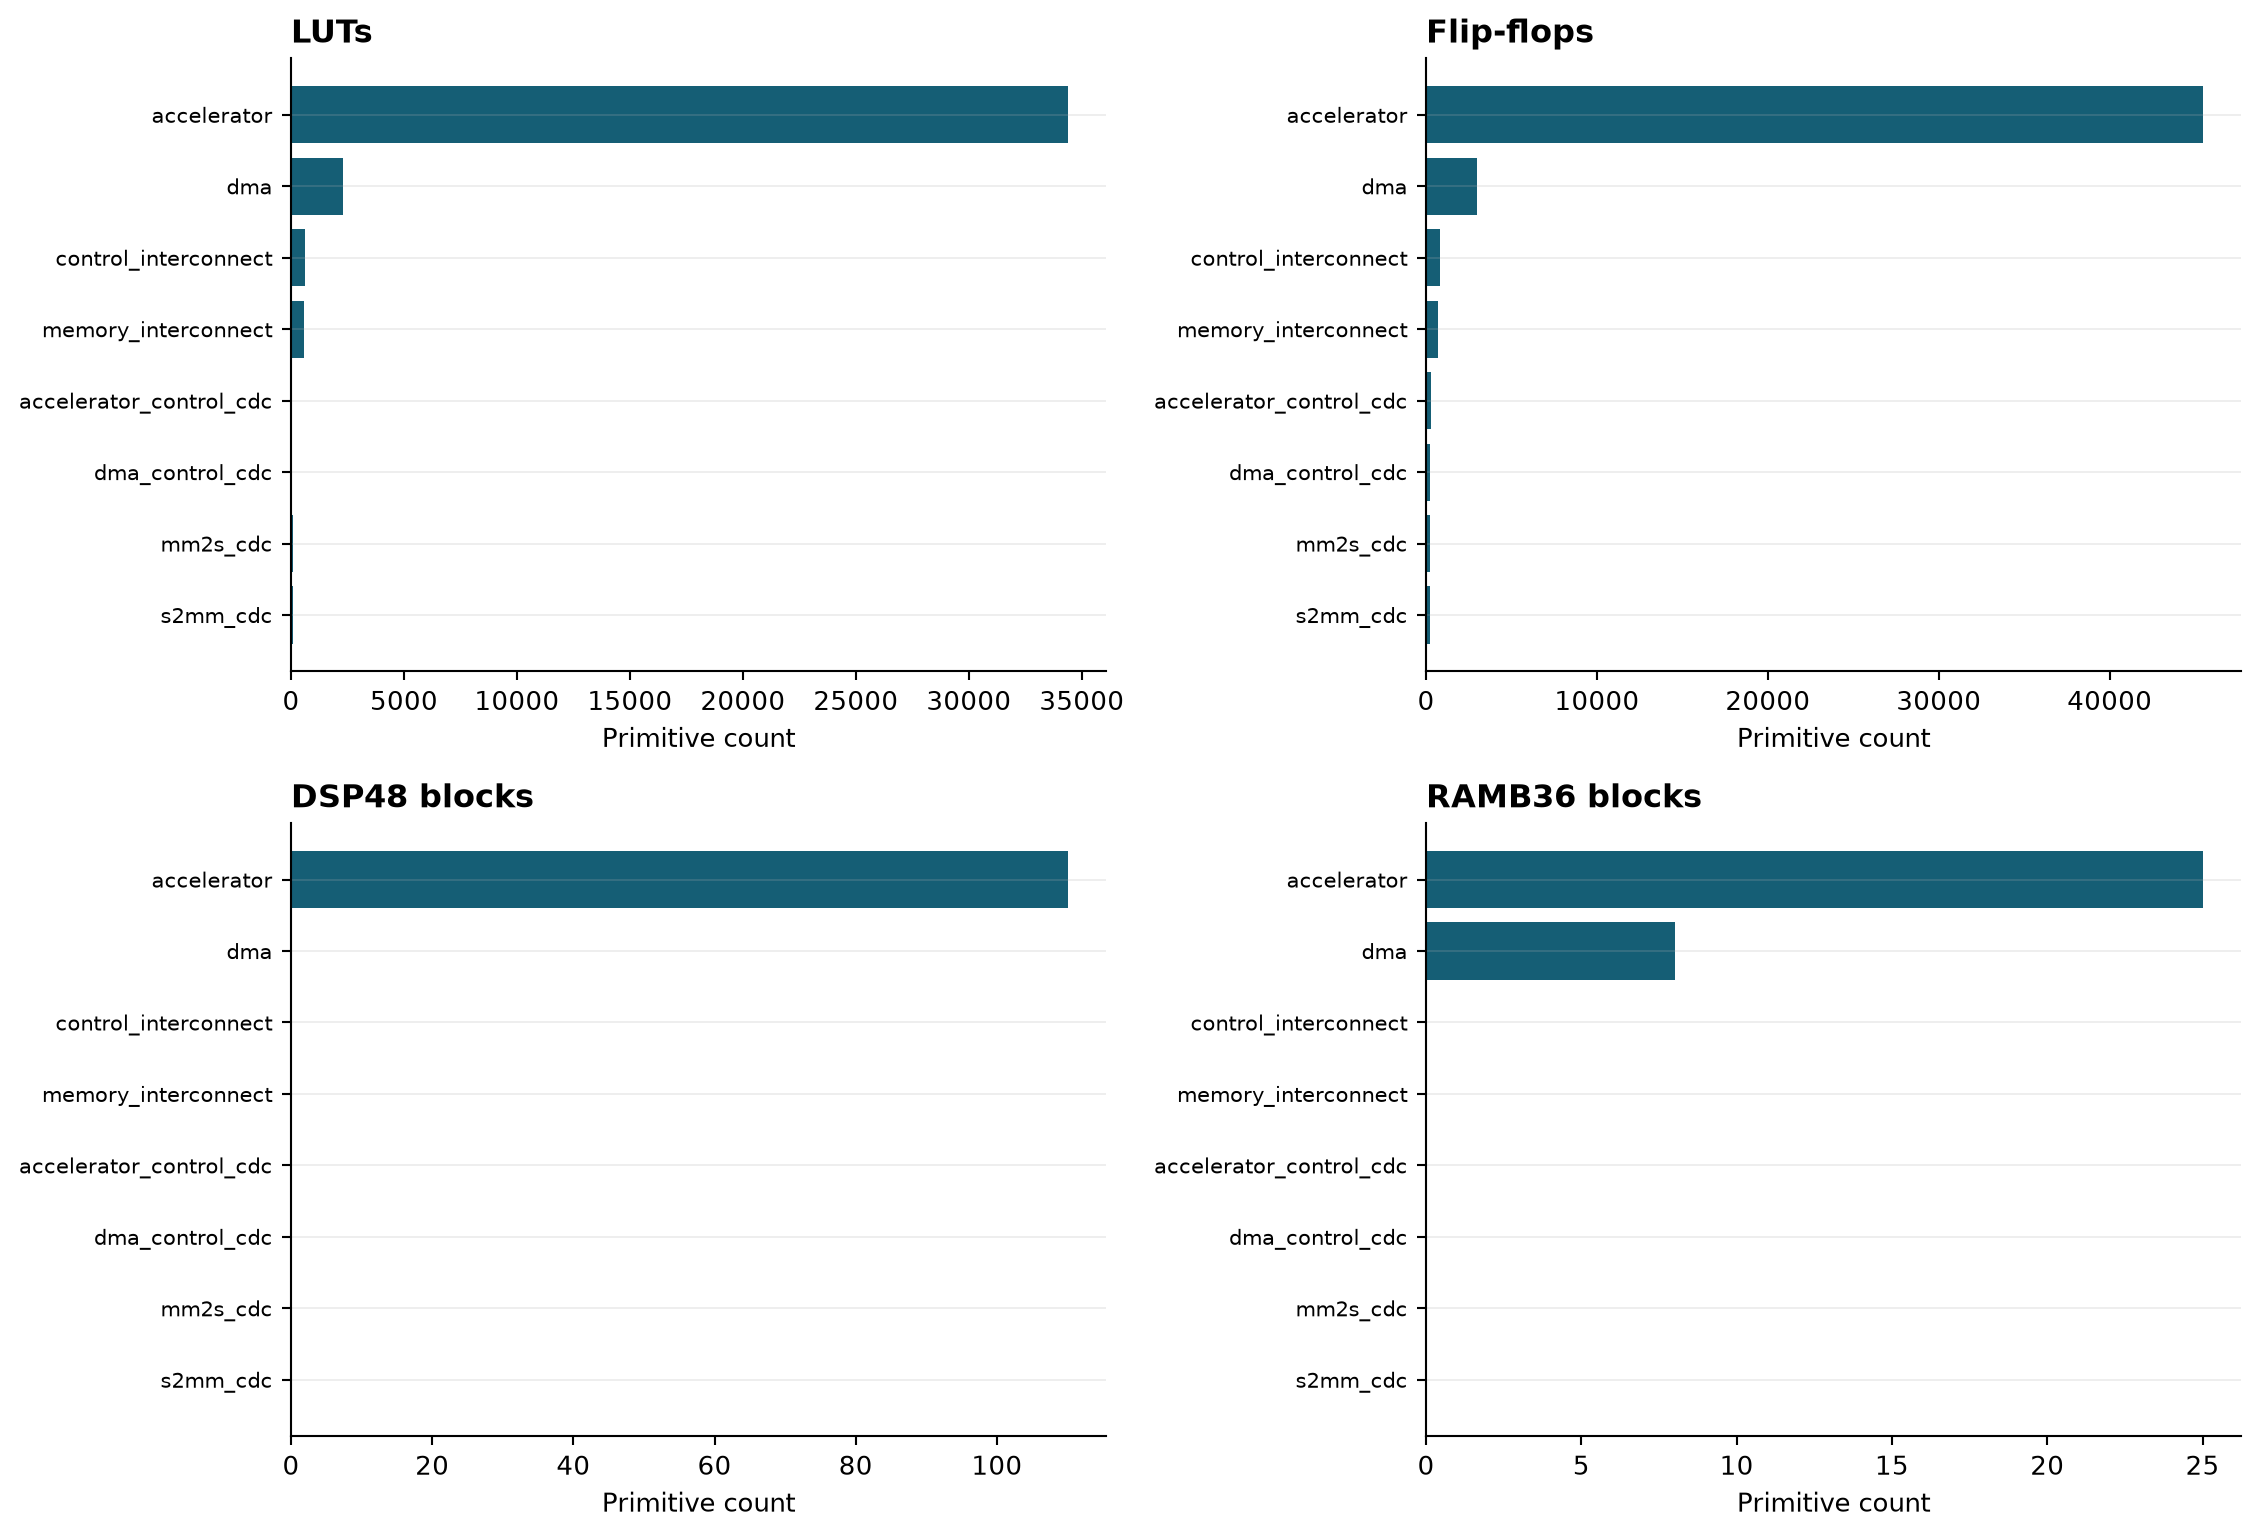
\includegraphics[width=0.98\textwidth,height=0.78\textheight,keepaspectratio]{plots/44_resource_hierarchy.png}
\end{center}
\clearpage
\section{DRC warning classification}
\begin{sloppypar}\small\textbf{Evidence:} C:\textbackslash{}\allowbreak{}Users\textbackslash{}\allowbreak{}Ross\textbackslash{}\allowbreak{}Downloads\textbackslash{}\allowbreak{}neuraedge--main\textbackslash{}\allowbreak{}neuraedge--main\textbackslash{}\allowbreak{}neuraedge\_\allowbreak{}universal\textbackslash{}\allowbreak{}outputs\textbackslash{}\allowbreak{}pynq\_\allowbreak{}full\textbackslash{}\allowbreak{}full\_\allowbreak{}drc.rpt\end{sloppypar}
\begin{center}
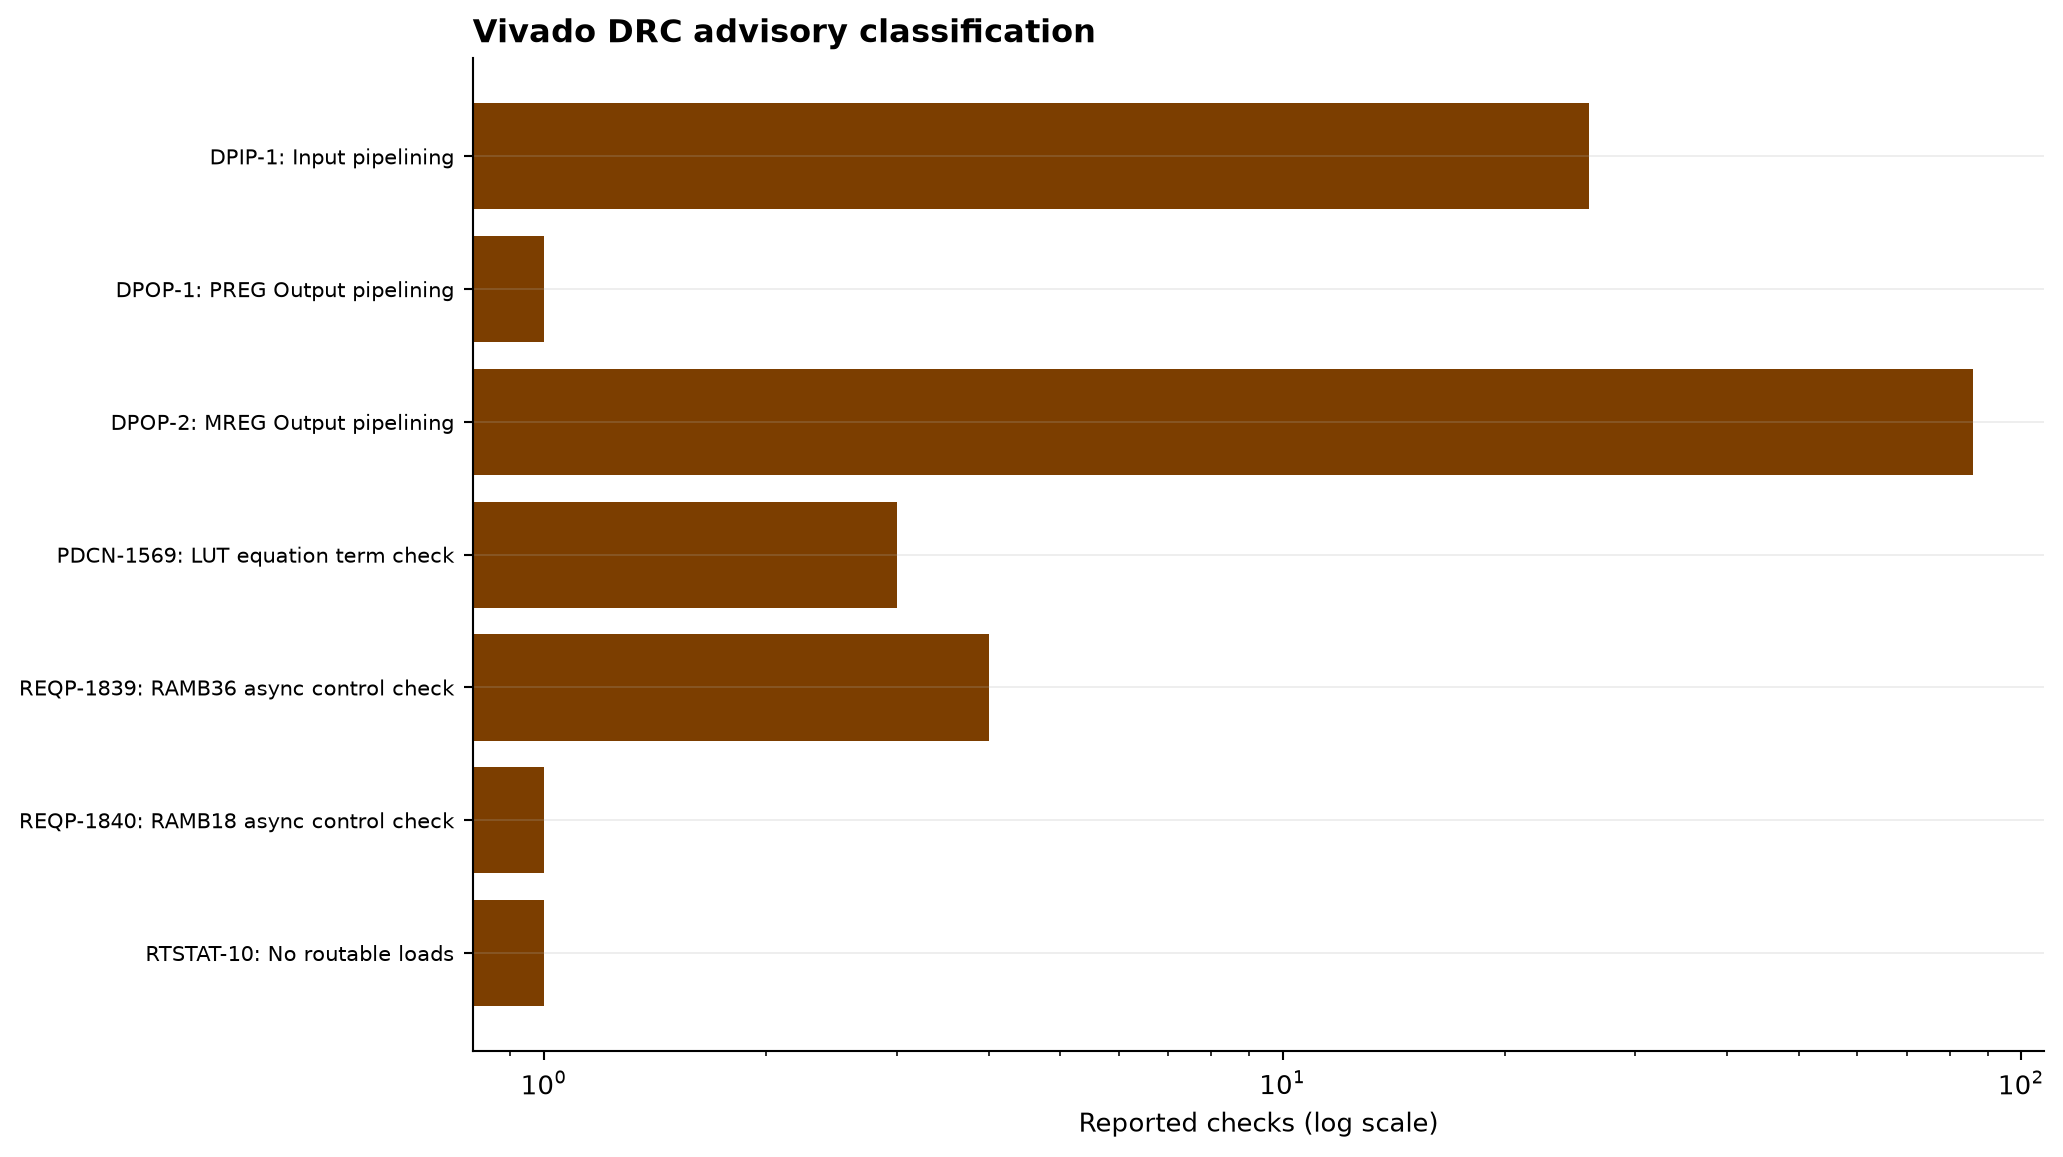
\includegraphics[width=0.98\textwidth,height=0.78\textheight,keepaspectratio]{plots/45_drc_classification.png}
\end{center}
\clearpage
\section{Clock-domain crossing classification}
\begin{sloppypar}\small\textbf{Evidence:} C:\textbackslash{}\allowbreak{}Users\textbackslash{}\allowbreak{}Ross\textbackslash{}\allowbreak{}Downloads\textbackslash{}\allowbreak{}neuraedge--main\textbackslash{}\allowbreak{}neuraedge--main\textbackslash{}\allowbreak{}neuraedge\_\allowbreak{}universal\textbackslash{}\allowbreak{}outputs\textbackslash{}\allowbreak{}pynq\_\allowbreak{}full\textbackslash{}\allowbreak{}full\_\allowbreak{}cdc.rpt\end{sloppypar}
\begin{center}
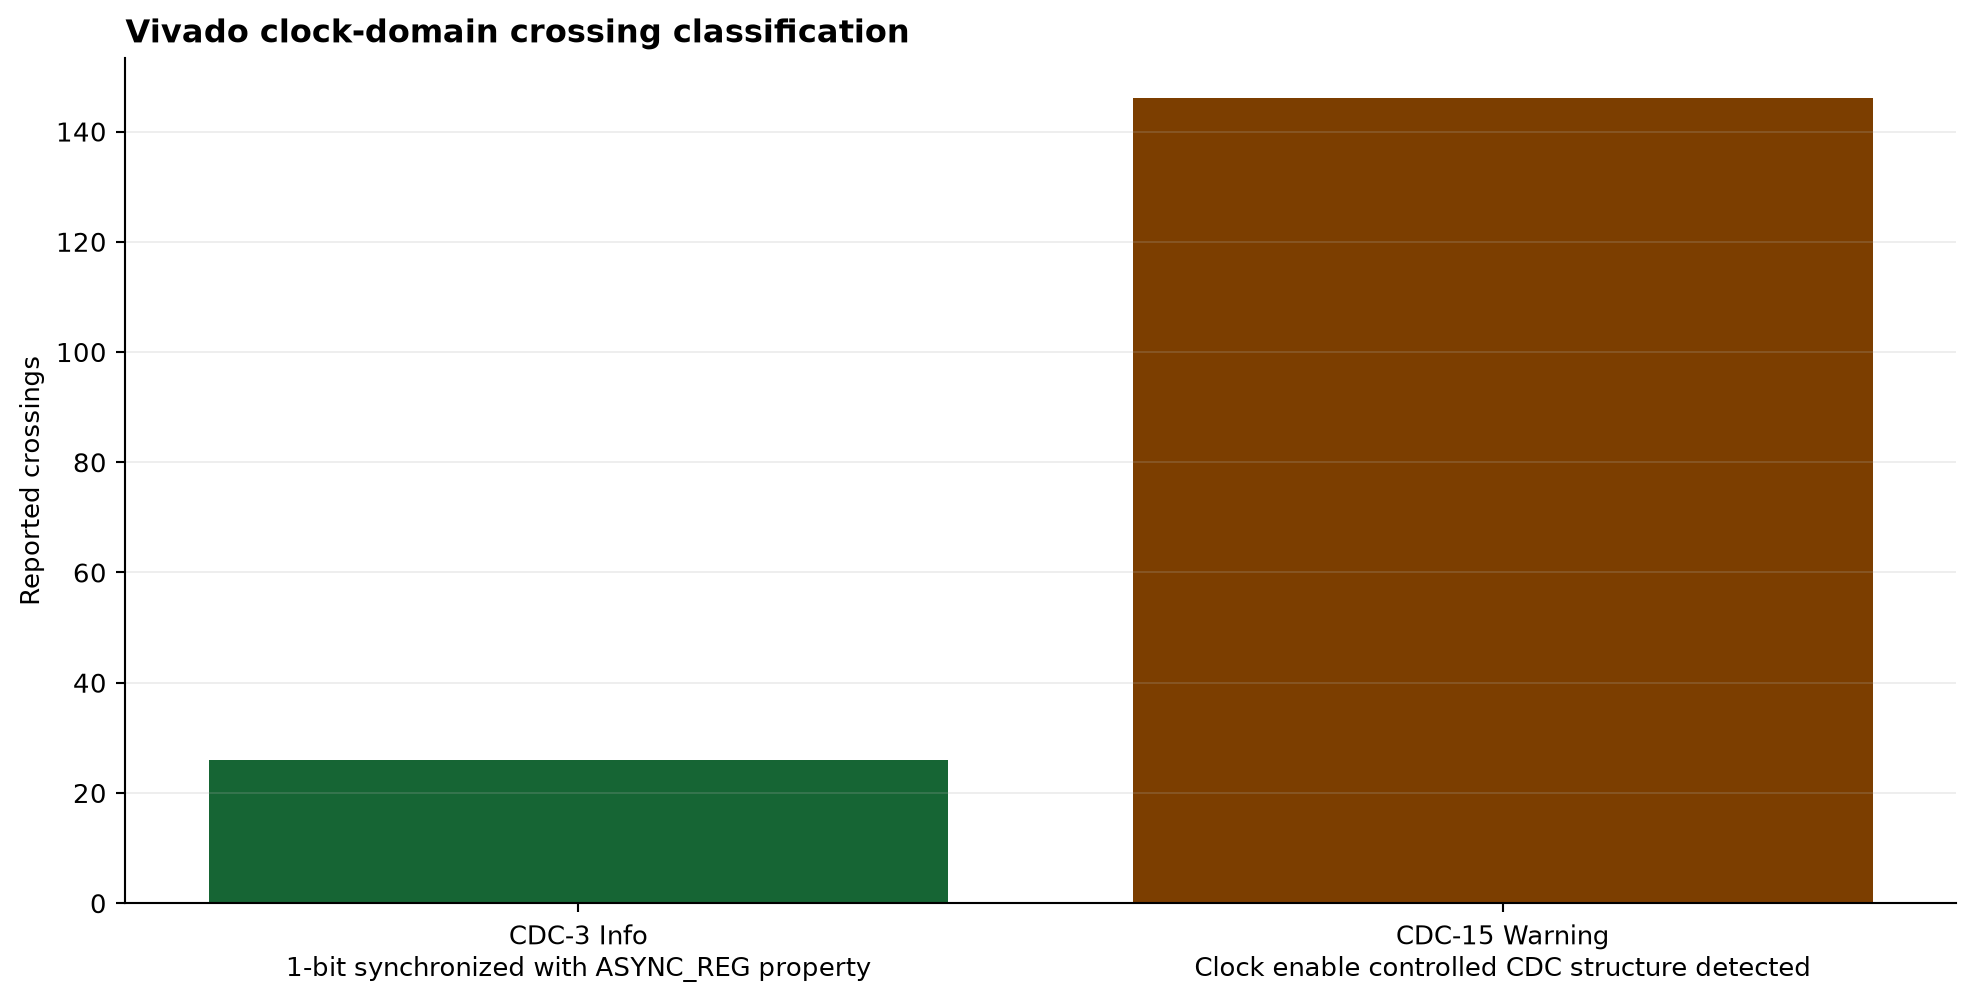
\includegraphics[width=0.98\textwidth,height=0.78\textheight,keepaspectratio]{plots/46_cdc_classification.png}
\end{center}
\clearpage
\section{Vectorless and SAIF-annotated power estimates}
\begin{sloppypar}\small\textbf{Evidence:} C:\textbackslash{}\allowbreak{}Users\textbackslash{}\allowbreak{}Ross\textbackslash{}\allowbreak{}Downloads\textbackslash{}\allowbreak{}neuraedge--main\textbackslash{}\allowbreak{}neuraedge--main\textbackslash{}\allowbreak{}neuraedge\_\allowbreak{}universal\textbackslash{}\allowbreak{}outputs\textbackslash{}\allowbreak{}pynq\_\allowbreak{}full\textbackslash{}\allowbreak{}full\_\allowbreak{}vectorless\_\allowbreak{}power.rpt;\allowbreak{} C:\textbackslash{}\allowbreak{}Users\textbackslash{}\allowbreak{}Ross\textbackslash{}\allowbreak{}Downloads\textbackslash{}\allowbreak{}neuraedge--main\textbackslash{}\allowbreak{}neuraedge--main\textbackslash{}\allowbreak{}neuraedge\_\allowbreak{}universal\textbackslash{}\allowbreak{}outputs\textbackslash{}\allowbreak{}power\_\allowbreak{}activity\_\allowbreak{}full\textbackslash{}\allowbreak{}vivado\_\allowbreak{}reports\textbackslash{}\allowbreak{}routed\_\allowbreak{}saif\_\allowbreak{}power.rpt;\allowbreak{} SAIF match 7\%   (9164/\allowbreak{}123250)\end{sloppypar}
\begin{center}
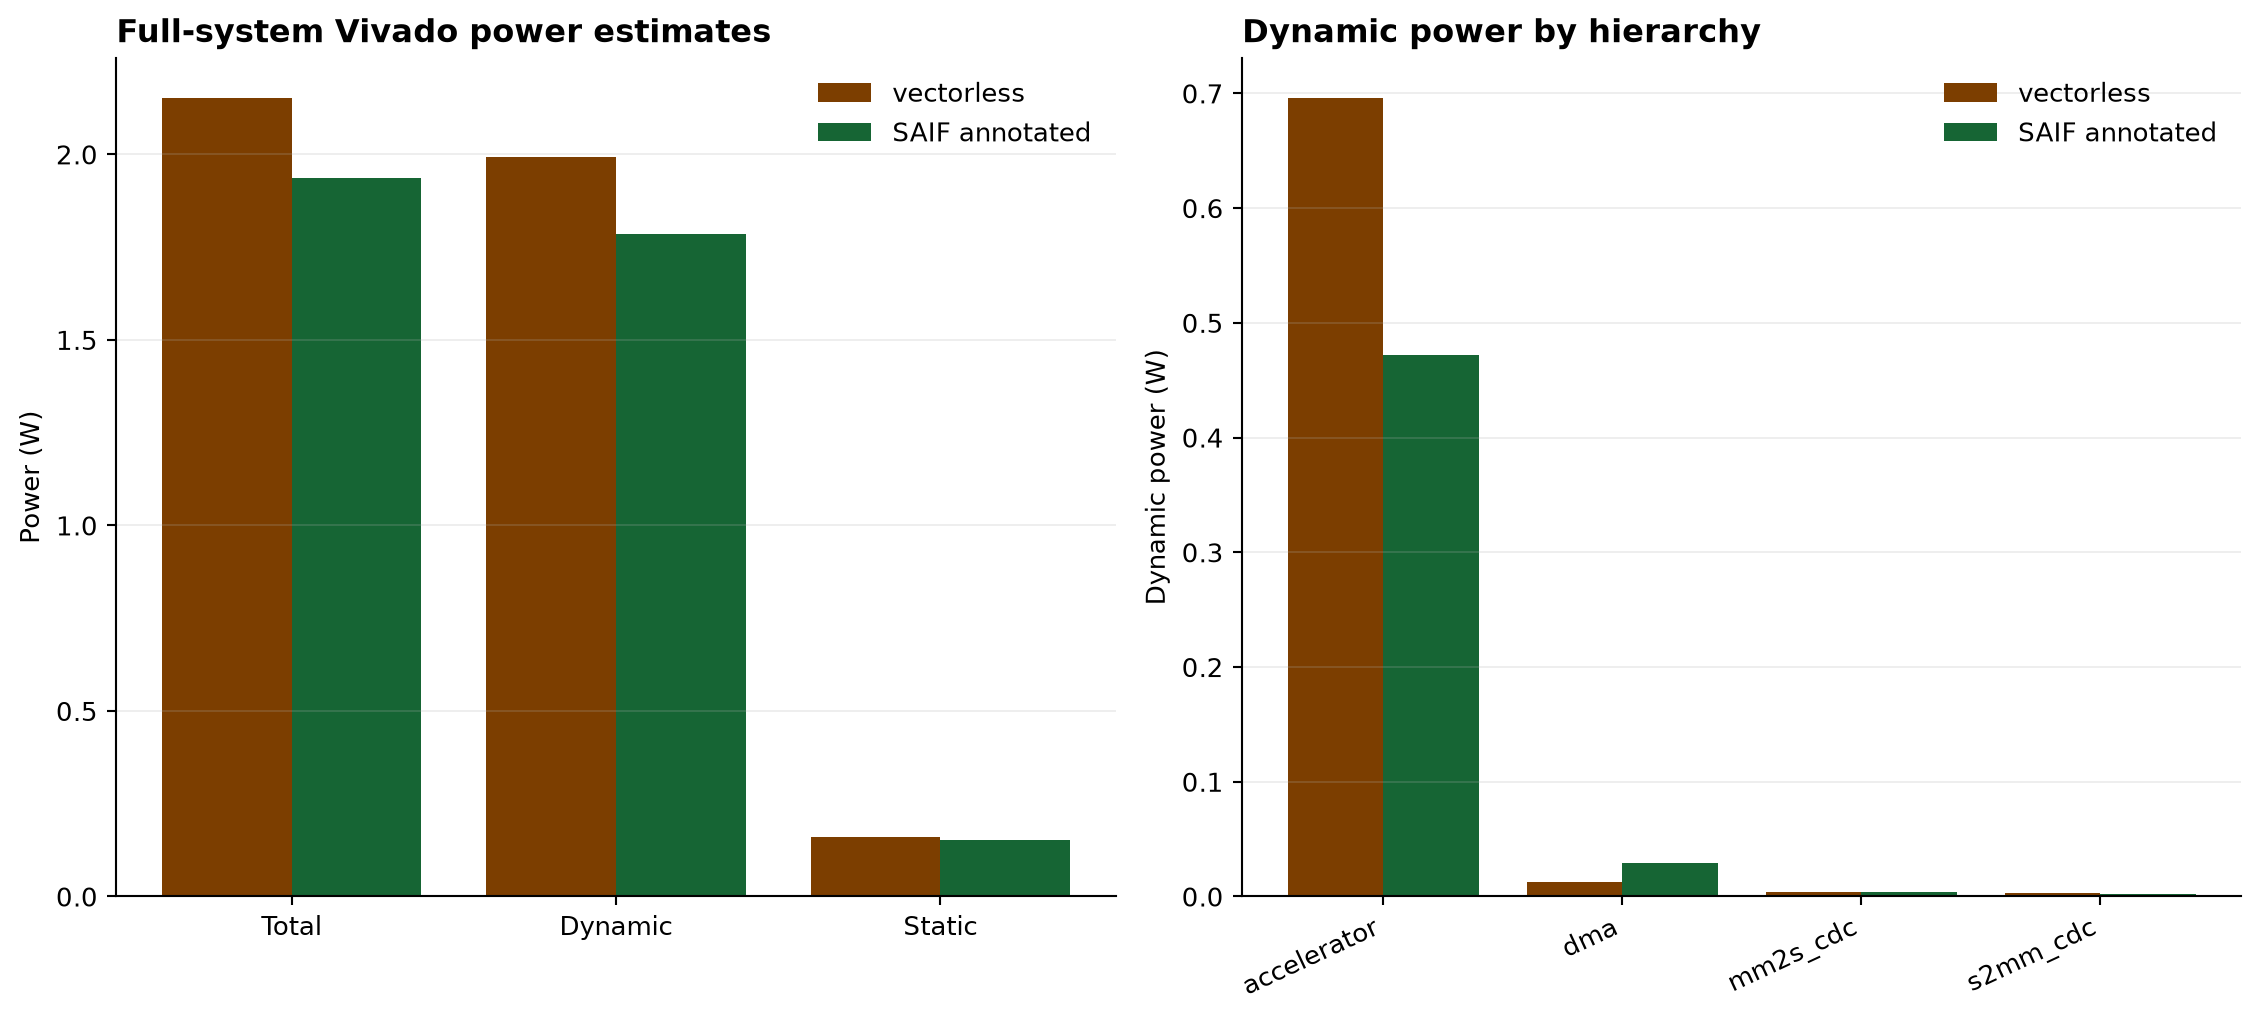
\includegraphics[width=0.98\textwidth,height=0.78\textheight,keepaspectratio]{plots/47_power_comparison.png}
\end{center}
\clearpage
\section{Power confidence and annotation coverage}
\begin{sloppypar}\small\textbf{Evidence:} C:\textbackslash{}\allowbreak{}Users\textbackslash{}\allowbreak{}Ross\textbackslash{}\allowbreak{}Downloads\textbackslash{}\allowbreak{}neuraedge--main\textbackslash{}\allowbreak{}neuraedge--main\textbackslash{}\allowbreak{}neuraedge\_\allowbreak{}universal\textbackslash{}\allowbreak{}outputs\textbackslash{}\allowbreak{}power\_\allowbreak{}activity\_\allowbreak{}full\textbackslash{}\allowbreak{}vivado\_\allowbreak{}reports\textbackslash{}\allowbreak{}routed\_\allowbreak{}saif\_\allowbreak{}power.rpt\end{sloppypar}
\begin{center}
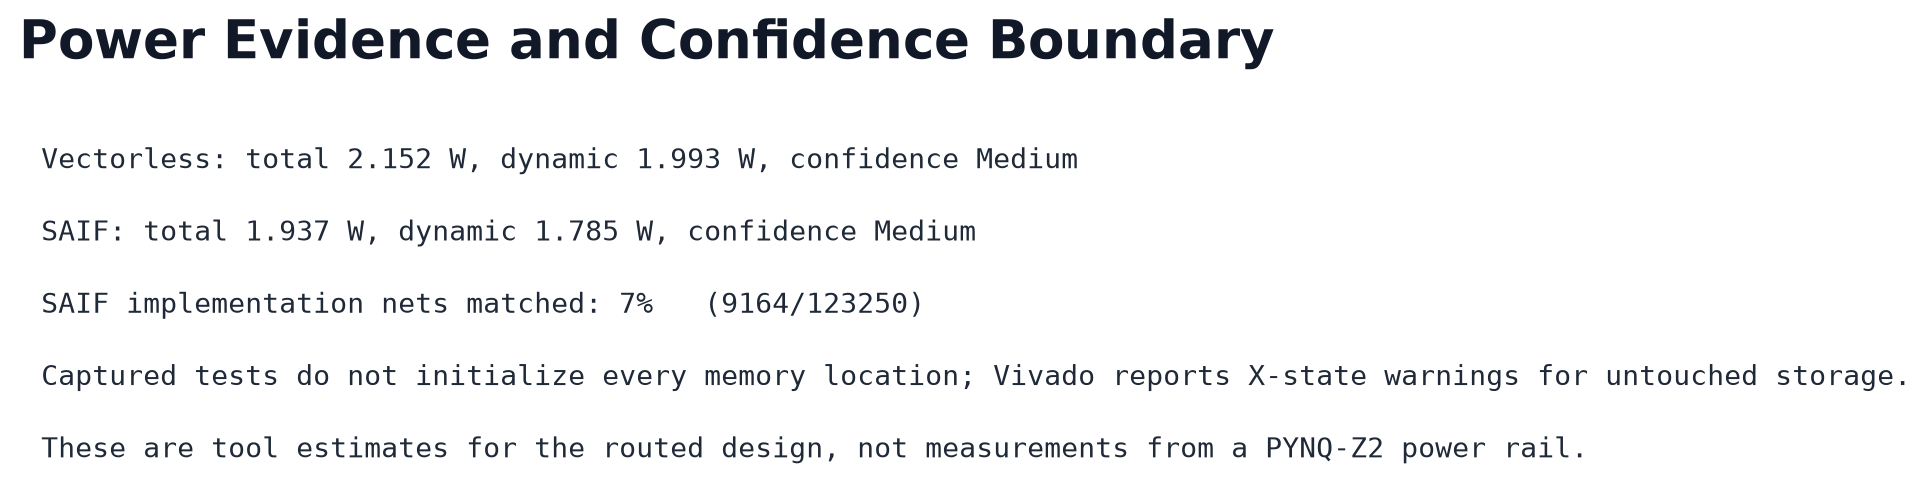
\includegraphics[width=0.98\textwidth,height=0.78\textheight,keepaspectratio]{plots/48_power_confidence.png}
\end{center}
\clearpage
\section{Routed timing path distribution}
\begin{sloppypar}\small\textbf{Evidence:} C:\textbackslash{}\allowbreak{}Users\textbackslash{}\allowbreak{}Ross\textbackslash{}\allowbreak{}Downloads\textbackslash{}\allowbreak{}neuraedge--main\textbackslash{}\allowbreak{}neuraedge--main\textbackslash{}\allowbreak{}neuraedge\_\allowbreak{}universal\textbackslash{}\allowbreak{}outputs\textbackslash{}\allowbreak{}pynq\_\allowbreak{}full\textbackslash{}\allowbreak{}full\_\allowbreak{}routed\_\allowbreak{}timing\_\allowbreak{}paths\_\allowbreak{}250.rpt\end{sloppypar}
\begin{center}
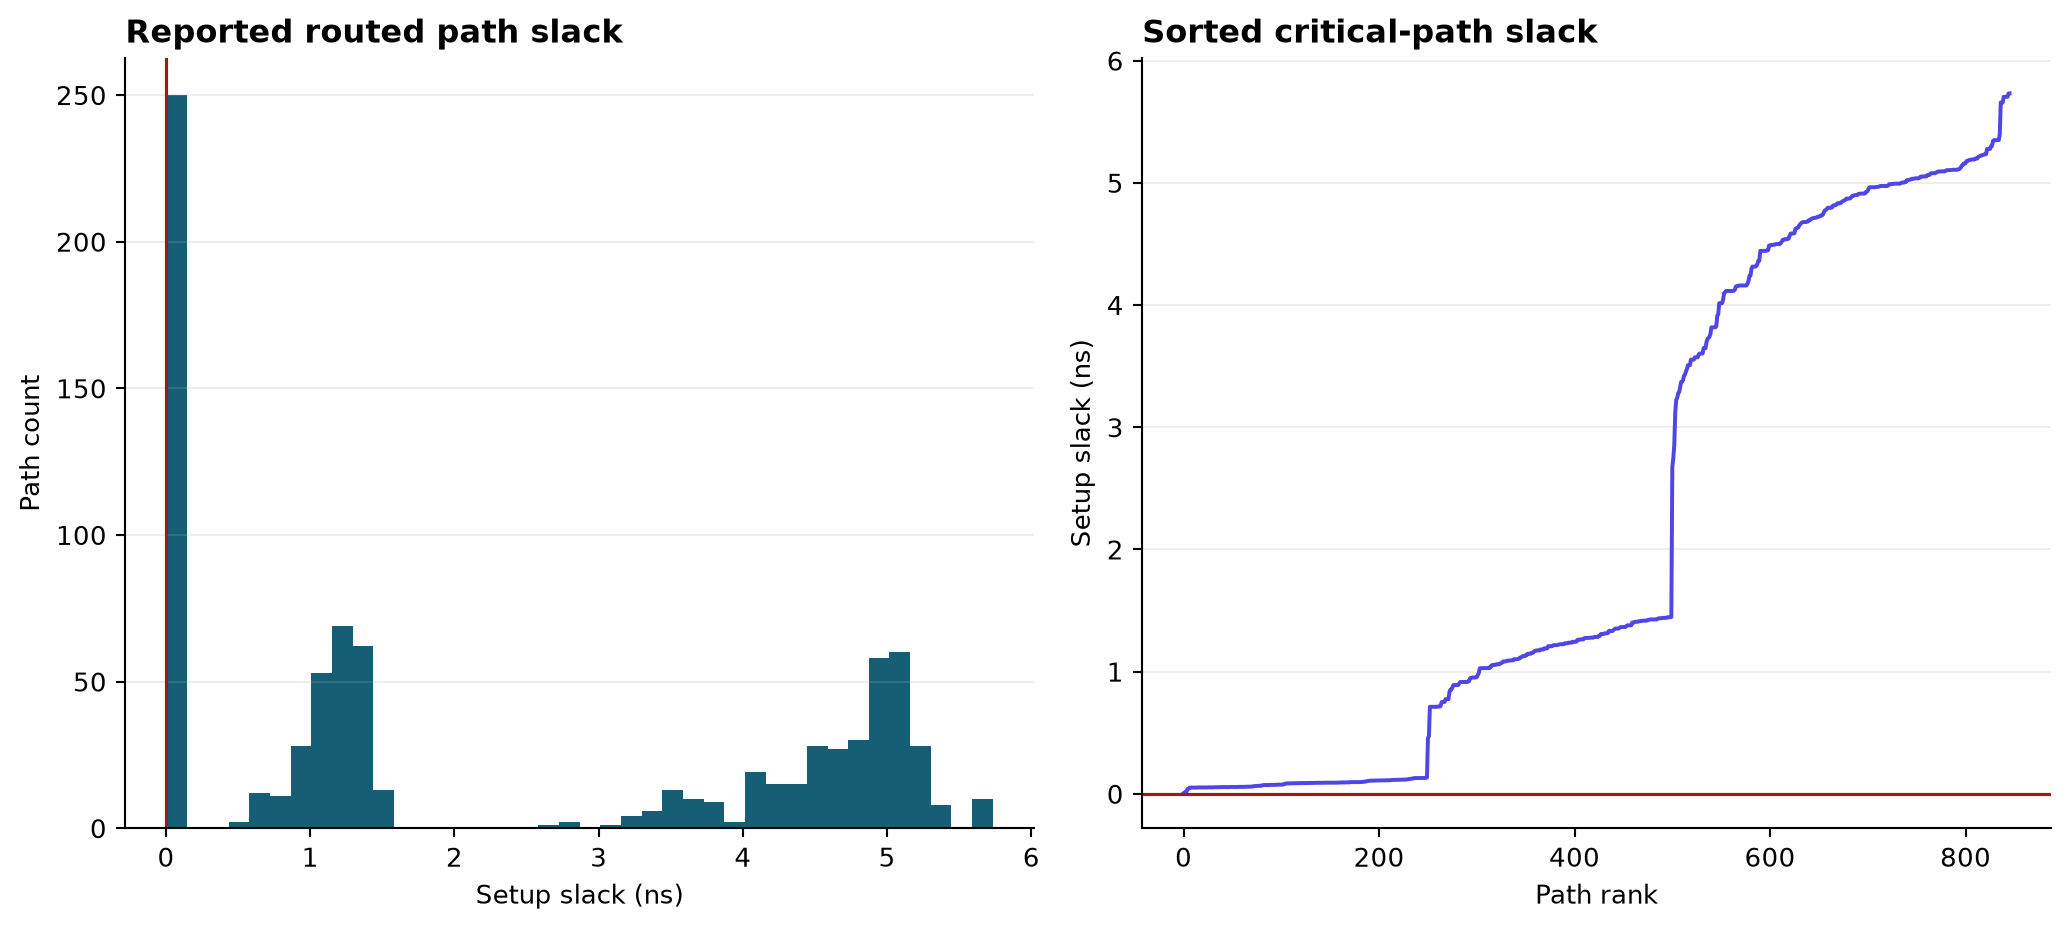
\includegraphics[width=0.98\textwidth,height=0.78\textheight,keepaspectratio]{plots/49_routed_timing.png}
\end{center}
\end{document}
